% Options for packages loaded elsewhere
\PassOptionsToPackage{unicode}{hyperref}
\PassOptionsToPackage{hyphens}{url}
\PassOptionsToPackage{dvipsnames,svgnames,x11names}{xcolor}
%
\documentclass[
  letterpaper,
  DIV=11,
  numbers=noendperiod]{scrreprt}

\usepackage{amsmath,amssymb}
\usepackage{iftex}
\ifPDFTeX
  \usepackage[T1]{fontenc}
  \usepackage[utf8]{inputenc}
  \usepackage{textcomp} % provide euro and other symbols
\else % if luatex or xetex
  \usepackage{unicode-math}
  \defaultfontfeatures{Scale=MatchLowercase}
  \defaultfontfeatures[\rmfamily]{Ligatures=TeX,Scale=1}
\fi
\usepackage{lmodern}
\ifPDFTeX\else  
    % xetex/luatex font selection
\fi
% Use upquote if available, for straight quotes in verbatim environments
\IfFileExists{upquote.sty}{\usepackage{upquote}}{}
\IfFileExists{microtype.sty}{% use microtype if available
  \usepackage[]{microtype}
  \UseMicrotypeSet[protrusion]{basicmath} % disable protrusion for tt fonts
}{}
\makeatletter
\@ifundefined{KOMAClassName}{% if non-KOMA class
  \IfFileExists{parskip.sty}{%
    \usepackage{parskip}
  }{% else
    \setlength{\parindent}{0pt}
    \setlength{\parskip}{6pt plus 2pt minus 1pt}}
}{% if KOMA class
  \KOMAoptions{parskip=half}}
\makeatother
\usepackage{xcolor}
\setlength{\emergencystretch}{3em} % prevent overfull lines
\setcounter{secnumdepth}{2}
% Make \paragraph and \subparagraph free-standing
\ifx\paragraph\undefined\else
  \let\oldparagraph\paragraph
  \renewcommand{\paragraph}[1]{\oldparagraph{#1}\mbox{}}
\fi
\ifx\subparagraph\undefined\else
  \let\oldsubparagraph\subparagraph
  \renewcommand{\subparagraph}[1]{\oldsubparagraph{#1}\mbox{}}
\fi

\usepackage{color}
\usepackage{fancyvrb}
\newcommand{\VerbBar}{|}
\newcommand{\VERB}{\Verb[commandchars=\\\{\}]}
\DefineVerbatimEnvironment{Highlighting}{Verbatim}{commandchars=\\\{\}}
% Add ',fontsize=\small' for more characters per line
\usepackage{framed}
\definecolor{shadecolor}{RGB}{241,243,245}
\newenvironment{Shaded}{\begin{snugshade}}{\end{snugshade}}
\newcommand{\AlertTok}[1]{\textcolor[rgb]{0.68,0.00,0.00}{#1}}
\newcommand{\AnnotationTok}[1]{\textcolor[rgb]{0.37,0.37,0.37}{#1}}
\newcommand{\AttributeTok}[1]{\textcolor[rgb]{0.40,0.45,0.13}{#1}}
\newcommand{\BaseNTok}[1]{\textcolor[rgb]{0.68,0.00,0.00}{#1}}
\newcommand{\BuiltInTok}[1]{\textcolor[rgb]{0.00,0.23,0.31}{#1}}
\newcommand{\CharTok}[1]{\textcolor[rgb]{0.13,0.47,0.30}{#1}}
\newcommand{\CommentTok}[1]{\textcolor[rgb]{0.37,0.37,0.37}{#1}}
\newcommand{\CommentVarTok}[1]{\textcolor[rgb]{0.37,0.37,0.37}{\textit{#1}}}
\newcommand{\ConstantTok}[1]{\textcolor[rgb]{0.56,0.35,0.01}{#1}}
\newcommand{\ControlFlowTok}[1]{\textcolor[rgb]{0.00,0.23,0.31}{#1}}
\newcommand{\DataTypeTok}[1]{\textcolor[rgb]{0.68,0.00,0.00}{#1}}
\newcommand{\DecValTok}[1]{\textcolor[rgb]{0.68,0.00,0.00}{#1}}
\newcommand{\DocumentationTok}[1]{\textcolor[rgb]{0.37,0.37,0.37}{\textit{#1}}}
\newcommand{\ErrorTok}[1]{\textcolor[rgb]{0.68,0.00,0.00}{#1}}
\newcommand{\ExtensionTok}[1]{\textcolor[rgb]{0.00,0.23,0.31}{#1}}
\newcommand{\FloatTok}[1]{\textcolor[rgb]{0.68,0.00,0.00}{#1}}
\newcommand{\FunctionTok}[1]{\textcolor[rgb]{0.28,0.35,0.67}{#1}}
\newcommand{\ImportTok}[1]{\textcolor[rgb]{0.00,0.46,0.62}{#1}}
\newcommand{\InformationTok}[1]{\textcolor[rgb]{0.37,0.37,0.37}{#1}}
\newcommand{\KeywordTok}[1]{\textcolor[rgb]{0.00,0.23,0.31}{#1}}
\newcommand{\NormalTok}[1]{\textcolor[rgb]{0.00,0.23,0.31}{#1}}
\newcommand{\OperatorTok}[1]{\textcolor[rgb]{0.37,0.37,0.37}{#1}}
\newcommand{\OtherTok}[1]{\textcolor[rgb]{0.00,0.23,0.31}{#1}}
\newcommand{\PreprocessorTok}[1]{\textcolor[rgb]{0.68,0.00,0.00}{#1}}
\newcommand{\RegionMarkerTok}[1]{\textcolor[rgb]{0.00,0.23,0.31}{#1}}
\newcommand{\SpecialCharTok}[1]{\textcolor[rgb]{0.37,0.37,0.37}{#1}}
\newcommand{\SpecialStringTok}[1]{\textcolor[rgb]{0.13,0.47,0.30}{#1}}
\newcommand{\StringTok}[1]{\textcolor[rgb]{0.13,0.47,0.30}{#1}}
\newcommand{\VariableTok}[1]{\textcolor[rgb]{0.07,0.07,0.07}{#1}}
\newcommand{\VerbatimStringTok}[1]{\textcolor[rgb]{0.13,0.47,0.30}{#1}}
\newcommand{\WarningTok}[1]{\textcolor[rgb]{0.37,0.37,0.37}{\textit{#1}}}

\providecommand{\tightlist}{%
  \setlength{\itemsep}{0pt}\setlength{\parskip}{0pt}}\usepackage{longtable,booktabs,array}
\usepackage{calc} % for calculating minipage widths
% Correct order of tables after \paragraph or \subparagraph
\usepackage{etoolbox}
\makeatletter
\patchcmd\longtable{\par}{\if@noskipsec\mbox{}\fi\par}{}{}
\makeatother
% Allow footnotes in longtable head/foot
\IfFileExists{footnotehyper.sty}{\usepackage{footnotehyper}}{\usepackage{footnote}}
\makesavenoteenv{longtable}
\usepackage{graphicx}
\makeatletter
\def\maxwidth{\ifdim\Gin@nat@width>\linewidth\linewidth\else\Gin@nat@width\fi}
\def\maxheight{\ifdim\Gin@nat@height>\textheight\textheight\else\Gin@nat@height\fi}
\makeatother
% Scale images if necessary, so that they will not overflow the page
% margins by default, and it is still possible to overwrite the defaults
% using explicit options in \includegraphics[width, height, ...]{}
\setkeys{Gin}{width=\maxwidth,height=\maxheight,keepaspectratio}
% Set default figure placement to htbp
\makeatletter
\def\fps@figure{htbp}
\makeatother

% Ignore commands that help with beamer spacing
\def\pause{}
\def\lspace{}
\def\pspace{}

% Tighter lists
\usepackage{enumitem}
\setlist{nosep}
\KOMAoption{captions}{tableheading}
\makeatletter
\@ifpackageloaded{tcolorbox}{}{\usepackage[skins,breakable]{tcolorbox}}
\@ifpackageloaded{fontawesome5}{}{\usepackage{fontawesome5}}
\definecolor{quarto-callout-color}{HTML}{909090}
\definecolor{quarto-callout-note-color}{HTML}{0758E5}
\definecolor{quarto-callout-important-color}{HTML}{CC1914}
\definecolor{quarto-callout-warning-color}{HTML}{EB9113}
\definecolor{quarto-callout-tip-color}{HTML}{00A047}
\definecolor{quarto-callout-caution-color}{HTML}{FC5300}
\definecolor{quarto-callout-color-frame}{HTML}{acacac}
\definecolor{quarto-callout-note-color-frame}{HTML}{4582ec}
\definecolor{quarto-callout-important-color-frame}{HTML}{d9534f}
\definecolor{quarto-callout-warning-color-frame}{HTML}{f0ad4e}
\definecolor{quarto-callout-tip-color-frame}{HTML}{02b875}
\definecolor{quarto-callout-caution-color-frame}{HTML}{fd7e14}
\makeatother
\makeatletter
\makeatother
\makeatletter
\@ifpackageloaded{bookmark}{}{\usepackage{bookmark}}
\makeatother
\makeatletter
\@ifpackageloaded{caption}{}{\usepackage{caption}}
\AtBeginDocument{%
\ifdefined\contentsname
  \renewcommand*\contentsname{Table of contents}
\else
  \newcommand\contentsname{Table of contents}
\fi
\ifdefined\listfigurename
  \renewcommand*\listfigurename{List of Figures}
\else
  \newcommand\listfigurename{List of Figures}
\fi
\ifdefined\listtablename
  \renewcommand*\listtablename{List of Tables}
\else
  \newcommand\listtablename{List of Tables}
\fi
\ifdefined\figurename
  \renewcommand*\figurename{Figure}
\else
  \newcommand\figurename{Figure}
\fi
\ifdefined\tablename
  \renewcommand*\tablename{Table}
\else
  \newcommand\tablename{Table}
\fi
}
\@ifpackageloaded{float}{}{\usepackage{float}}
\floatstyle{ruled}
\@ifundefined{c@chapter}{\newfloat{codelisting}{h}{lop}}{\newfloat{codelisting}{h}{lop}[chapter]}
\floatname{codelisting}{Listing}
\newcommand*\listoflistings{\listof{codelisting}{List of Listings}}
\makeatother
\makeatletter
\@ifpackageloaded{caption}{}{\usepackage{caption}}
\@ifpackageloaded{subcaption}{}{\usepackage{subcaption}}
\makeatother
\makeatletter
\@ifpackageloaded{tcolorbox}{}{\usepackage[skins,breakable]{tcolorbox}}
\makeatother
\makeatletter
\@ifundefined{shadecolor}{\definecolor{shadecolor}{rgb}{.97, .97, .97}}
\makeatother
\makeatletter
\makeatother
\makeatletter
\makeatother
\ifLuaTeX
  \usepackage{selnolig}  % disable illegal ligatures
\fi
\IfFileExists{bookmark.sty}{\usepackage{bookmark}}{\usepackage{hyperref}}
\IfFileExists{xurl.sty}{\usepackage{xurl}}{} % add URL line breaks if available
\urlstyle{same} % disable monospaced font for URLs
\hypersetup{
  pdftitle={Statistics for Life Sciences},
  pdfauthor={Dr.~Devan Becker},
  colorlinks=true,
  linkcolor={blue},
  filecolor={Maroon},
  citecolor={Blue},
  urlcolor={Blue},
  pdfcreator={LaTeX via pandoc}}

\title{Statistics for Life Sciences}
\usepackage{etoolbox}
\makeatletter
\providecommand{\subtitle}[1]{% add subtitle to \maketitle
  \apptocmd{\@title}{\par {\large #1 \par}}{}{}
}
\makeatother
\subtitle{Course Notes for ST231, Sprummer 2023}
\author{Dr.~Devan Becker}
\date{2023-06-20}

\begin{document}
\maketitle
\ifdefined\Shaded\renewenvironment{Shaded}{\begin{tcolorbox}[frame hidden, sharp corners, interior hidden, borderline west={3pt}{0pt}{shadecolor}, boxrule=0pt, enhanced, breakable]}{\end{tcolorbox}}\fi

\renewcommand*\contentsname{Table of contents}
{
\hypersetup{linkcolor=}
\setcounter{tocdepth}{2}
\tableofcontents
}
\bookmarksetup{startatroot}

\hypertarget{introduction}{%
\chapter*{Introduction}\label{introduction}}
\addcontentsline{toc}{chapter}{Introduction}

\markboth{Introduction}{Introduction}

These course notes structured to coincide with Baldi and Moore's The
Basic Practice of Statistics in the Life Sciences, 4th edition. However,
I am working towards making them self-contained in order to provide
these notes as an Open Educational Resources. In doing so, I will also
borrow from OpenIntro Statistics for the Biomedical and Life Sciences,
with attribution. As such, these resources have the same license (see
the end of this page), except for those elements that are still present
from Baldi \& Moore (mainly exercises, which are being removed as I go).

\hypertarget{completion-progress}{%
\section*{Completion Progress}\label{completion-progress}}
\addcontentsline{toc}{section}{Completion Progress}

\markright{Completion Progress}

These notes are still in progress.

\begin{itemize}
\tightlist
\item
  Ch01 has been edited since the version posted in class.
\item
  Ch02-Ch09 are the versions posted to MyLS for this semester.

  \begin{itemize}
  \tightlist
  \item
    There may be missing images due to copyright concerns.
  \end{itemize}
\item
  Ch10-13 are updated for this book, and are the course notes I will
  refer to moving forward.
\item
  Ch14+ are direct copies of old notes and need editing, which may
  involve addition of new material.

  \begin{itemize}
  \tightlist
  \item
    If you read ahead, you may need to re-read later.
  \end{itemize}
\end{itemize}

\hypertarget{helpful-information}{%
\section*{Helpful Information}\label{helpful-information}}
\addcontentsline{toc}{section}{Helpful Information}

\markright{Helpful Information}

\begin{itemize}
\tightlist
\item
  Text: Bald \& Moore: The practice of statistics in the life sciences.

  \begin{itemize}
  \tightlist
  \item
    \emph{Recommended}, not required.
  \item
    Copy available in the library. Old versions work fine.\lspace
  \end{itemize}
\item
  Alternate (free) text (trialing):

  \begin{itemize}
  \tightlist
  \item
    \href{https://www.openintro.org/book/biostat/}{OpenIntro Statistics
    for Life Sciences}
  \end{itemize}
\end{itemize}

The textbook for this course is recommended but not required. We will
not be using questions directly from the textbook so it's fine if you
have an old version. Instead, you can just use it as a reference for
extra information about any of the course topics.

I've also included an alternate textbook. If you use this, please share
your experience with me so that I know whether I could switch to this
free textbook!.

\hypertarget{learning-outcomes}{%
\section*{Learning Outcomes}\label{learning-outcomes}}
\addcontentsline{toc}{section}{Learning Outcomes}

\markright{Learning Outcomes}

\begin{itemize}
\tightlist
\item
  Critically appraise \textbf{published articles} in health sciences
  research.\lspace
\item
  Use \textbf{industry standard tools} to apply \textbf{basic
  statistical concepts} to \textbf{real-world problems}.\lspace
\item
  Understand the use and application of \textbf{statistical techniques}
  such as descriptive and inferential statistics.
\end{itemize}

\hypertarget{accessing-materials}{%
\section*{Accessing Materials}\label{accessing-materials}}
\addcontentsline{toc}{section}{Accessing Materials}

\markright{Accessing Materials}

\begin{itemize}
\tightlist
\item
  Lectures posted on MyLS\lspace
\item
  RStudio

  \begin{itemize}
  \tightlist
  \item
    Free, open-source interface to the R programming language.\lspace
  \end{itemize}
\item
  Syzygy Jupyter (JuPyteR) Notebooks

  \begin{itemize}
  \tightlist
  \item
    Free, \textbf{web-based} service for WLU students
  \item
    No need to install R on your own computer\lspace
  \end{itemize}
\end{itemize}

You can use either RStudio or syzygy for this course, RStudio has many
fantastic bells and whistles that help you produce results and reports,
whereas syzygy has an online interface and makes it easy to use without
installing R on your own computer.

For lectures, I will be using VSCode, which is the main program that I
use because it works well with python and R, as well as other languages
that I need. I will switch to RStudio for many demonstrations just to
show you how it works because this is the program that most people who
do statistics will use. I will occasionally demonstrate some concepts
using Jupyter notebooks because this is another common way that people
do statistics and data science. You will not be tested on the features
of Rtudio, VSCode or Jupyter notebooks, but mastery of RStudio will be
extremely helpful for all future data analysis tasks beyond this course.

This work is licensed under a Creative Commons Attribution-ShareAlike
4.0 Unported License.

\part{Pre-Midterm}

\hypertarget{picturing-distributions-with-graphs}{%
\chapter{Picturing Distributions with
Graphs}\label{picturing-distributions-with-graphs}}

\hypertarget{introduction-1}{%
\section{Introduction}\label{introduction-1}}

\hypertarget{defining-statistics}{%
\subsection{Defining ``Statistics''}\label{defining-statistics}}

My definition: Statistics is the study of \textbf{variance} (or
uncertainty).

\begin{itemize}
\tightlist
\item
  The big question: is 1 \textbf{statistically different} from 100?

  \begin{itemize}
  \tightlist
  \item
    1 vs.~100 apples? Yes.
  \item
    1 vs.~100 atoms in an apple? No.
  \end{itemize}
\end{itemize}

Many definitions of ``statistics'' are something along the lines of
``methods for dealing with data''. This completely misses out on
theoretical statistics, and makes it seem like statistics is a
collection of recipes stating ``if you have this data, use this
method''. I think a better definition of statistics is that it's the
study of variance, whether that means studying the theoretical
properties of variance or trying to explain variance in a particular
data set.

I like to ask the question: ``is 1 statistically different from 100''.
It may seem like they are obviously different numbers, but we can't know
that without the context. If you're comparing numbers of apples, then
yes, one apple is very different from 100 apples. However, if we're
looking at numbers of of atoms per apple, then one and 100 are both
imperceptible numbers of atoms and thus we might say they're practically
the same. The difference in these two examples is the scale, and
variance is a fantastic way to measure the scales of things. In my
opinion, the main thing we will learn in this course is how to tell
whether to numbers are different, \emph{given the scale of those two
numbers.} Another popular definition for statistics is ``putting numbers
in context'', and by ``in context'' they mean ``relative to their
variance''.

In my lecture notes, I use \textbf{bold font} for anything that you will
be expected to be able to explain or define. You won't necessarily see a
full definition the first time you see a word in bold, but by the
midterm/final it is something I expect you to know. A good way to study
in this course is to keep a glossary of all of the words I've put in
bold, with a definition file/note that you update as we learn more about
that concept. And, of course, write a description as if you're teaching
someone else!

\hypertarget{why-study-variance}{%
\subsection{Why study variance?}\label{why-study-variance}}

\begin{itemize}
\tightlist
\item
  Give context to different numbers.

  \begin{itemize}
  \tightlist
  \item
    The size of the difference depends on the context.
  \end{itemize}
\item
  We need to know \emph{how} and \emph{why} we were wrong.

  \begin{itemize}
  \tightlist
  \item
    \emph{How}: What is the magnitude of the difference?
  \item
    \emph{Why}: Are we missing relationships? Bad sampling? Fundamental
    randomness?
  \end{itemize}
\end{itemize}

Variance is information!

Variance comes from many sources. We might just be doing something wrong
and missing out on important feature of our data, we might be collecting
the data in a biased or incorrect way, or there might be some
fundamental part of the problem that we will never be able to measure
perfectly, and so the variance that we calculated may already be the
smallest possible variance for this problem.

I like to say that variance is information. Suppose we're trying to
figure out the heights of undergraduate students. We can calculate an
average height, but it is entirely possible that nobody in our data set
has a height that is exactly equally to the average height. We would
want to quantify how much variation there is around that average height.
If our sample includes a basketball team, then, this is variation due to
some thing that we could have measured. In other words, the variation in
our data can be explained by including another perspective. Once we have
that perspective and we were included in our analysis are variance
should be smaller, and therefore we have extracted more information. As
we gain more information about our data, the variance in our estimate
goes down - this is why I say that variance is information! Or, rather,
variance is hiding information.

\hypertarget{descriptive-versus-inferential-statistics}{%
\subsection{Descriptive Versus Inferential
Statistics}\label{descriptive-versus-inferential-statistics}}

\begin{itemize}
\tightlist
\item
  \textbf{Descriptive statistics} are used to explore the data.

  \begin{itemize}
  \tightlist
  \item
    Graphs/figures
  \item
    Numbers
  \end{itemize}
\item
  \textbf{Inferential statistics} relate our data to the
  \textbf{population}.

  \begin{itemize}
  \tightlist
  \item
    Must have a good \textbf{sample} first!
  \item
    Our sample has a mean. The population has a mean. How different do
    we expect them to be?

    \begin{itemize}
    \tightlist
    \item
      \textbf{how different}
    \end{itemize}
  \end{itemize}
\end{itemize}

In this course, we will learn about two classes of statistics.
Descriptive statistics are the ones that we used to describe the sample
that we obtained. This can include things like the mean/median/mode, the
variance or the interquartile range, as well as bar charts, histograms
box, plots, etc.

Inferential statistics are numbers that we calculate because we think
have a relationship to the population. For instance, if we calculate the
mean of our data, and we trust that our sample is good, then we expect
this sample mean to be somewhat close to the population mean. Any time
in this course I talk about the difference between two things, I will
always mean ``with reference to a measure of variance''. In this
example, we have a sample mean as well as some measure of its variance,
and this variance tells us how similar we expect the sample mean to be
to the population mean. If we have a small sample variance, it means
that we have a lot of information about the population mean. Variance
contains information that we haven't learned yet!\footnote{It is worth
  noting that there is also variance that isn't information, and there's
  information that we'll never have access to. Variance is an
  opportunity to learn, but there's almost always a limit to how much we
  can learn.}

In this course, we're going to start by talking about descriptive
statistics and work our way to inferential statistics.

\hypertarget{descriptive-statistics-plots-and-graphs}{%
\section{Descriptive Statistics: Plots and
Graphs}\label{descriptive-statistics-plots-and-graphs}}

\hypertarget{the-palmer-penguins-data}{%
\subsection{The Palmer Penguins Data}\label{the-palmer-penguins-data}}

Let me introduce you to a dataset that I'm going to be returning to
throughout the semester. This is called the Palmer penguins data, end it
contains information on penguins from several islands in Antarctica. In
the slides, I use some fancier code to only show some of the data, but
I'll display the full data set with simpler code below:

\begin{Shaded}
\begin{Highlighting}[]
\FunctionTok{library}\NormalTok{(palmerpenguins)}
\FunctionTok{head}\NormalTok{(}\FunctionTok{as.data.frame}\NormalTok{(penguins))}
\end{Highlighting}
\end{Shaded}

\begin{verbatim}
  species    island bill_length_mm bill_depth_mm flipper_length_mm body_mass_g
1  Adelie Torgersen           39.1          18.7               181        3750
2  Adelie Torgersen           39.5          17.4               186        3800
3  Adelie Torgersen           40.3          18.0               195        3250
4  Adelie Torgersen             NA            NA                NA          NA
5  Adelie Torgersen           36.7          19.3               193        3450
6  Adelie Torgersen           39.3          20.6               190        3650
     sex year
1   male 2007
2 female 2007
3 female 2007
4   <NA> 2007
5 female 2007
6   male 2007
\end{verbatim}

\begin{itemize}
\tightlist
\item
  Species can be Adelie, Gentoo, or Chinstrap
\item
  Sex can be male or female\footnote{A note on gender/sexuality/biology:
    penguins, especially Chinstrap and Gentoo penguins, don't have
    particularly strong gender roles, and
    \href{https://sites.tufts.edu/museumstudents/2021/02/22/whats-with-all-the-gay-penguins/}{often
    form same-sex couples}. In this course, I will use the term ``sex''
    to mean ``biosex'', rather than ``gender'', to indicate that we're
    looking at morphological differences due to XX and XY chromosomes.}
\item
  Bill Length is measured in millimetres
\item
  Body Mass is measured in grams
\item
  Not shown: Island (one of three), bill depth (mm), flipper length
  (mm), year.
\end{itemize}

These data are really nice for teaching statistics because we can look
at what factors contribute to body mass (since it's easier to measure
the length of a beak than it is to weigh a live penguin), or we can try
to determine biosex using these measurements (since penguins normally
have no external genitalia, but have other morphological differences).
We can also fit a model to determine the species of each penguin so that
we can get a full picture of what makes each species unique! All of
these are examples of statistical analyses that we will cover in this
course.

\hypertarget{types-of-variables}{%
\subsection{Types of Variables}\label{types-of-variables}}

\begin{Shaded}
\begin{Highlighting}[]
\NormalTok{penguins[, }\FunctionTok{c}\NormalTok{(}\StringTok{"species"}\NormalTok{, }\StringTok{"sex"}\NormalTok{, }\StringTok{"body\_mass\_g"}\NormalTok{)] }\SpecialCharTok{|\textgreater{}}
    \FunctionTok{head}\NormalTok{() }\SpecialCharTok{|\textgreater{}}
\NormalTok{    knitr}\SpecialCharTok{::}\FunctionTok{kable}\NormalTok{()}
\end{Highlighting}
\end{Shaded}

\begin{longtable}[]{@{}llr@{}}
\toprule\noalign{}
species & sex & body\_mass\_g \\
\midrule\noalign{}
\endhead
\bottomrule\noalign{}
\endlastfoot
Adelie & male & 3750 \\
Adelie & female & 3800 \\
Adelie & female & 3250 \\
Adelie & NA & NA \\
Adelie & female & 3450 \\
Adelie & male & 3650 \\
\end{longtable}

\begin{itemize}
\tightlist
\item
  Species is \textbf{categorical}

  \begin{itemize}
  \tightlist
  \item
    Mutually exclusive categories.
  \end{itemize}
\item
  Sex is \textbf{binary}\footnote{Possibly categorical if there are any
    penguins with chromosomal abnormalities.}

  \begin{itemize}
  \tightlist
  \item
    One or the other
  \item
    Special case of categorical with 2 possibilities
  \end{itemize}
\item
  Body mass is \textbf{quantitative}

  \begin{itemize}
  \tightlist
  \item
    It's a number (quantity)
  \end{itemize}
\end{itemize}

The type of variable is extremely important for choosing the right
summary of the data.

\textbf{Categorical variables} consist of two or more mutually exclusive
categories, that is, each observation has a label and nothing has more
than one label. Categorical variables may be \textbf{ordered} (such as
``low'', ``medium'', and ``high'') or \textbf{unordered} (such as names
or student numbers; putting names in alphabetical order is not usually
meaningful for summarising the data or doing the analysis).

This distinction of ``\textbf{ordered}'' versus ``\textbf{unordered}''
matters to determine what visualization or model you might want to use
to compare data within categories. For instance, we might want to see
the change in response to a ``low'' treatment compared to a ``medium''
or ``high'' treatment, where we fully expect the response to the
treatment to be lower for ``low'' treatment and higher for ``high''. In
contrast, suppose we knew the patients' occupations. We have no
expectation that the treatment reponse in the ``electrician'' group is
lower or higher than any other group, because there's no logical
ordering to occupation.\footnote{We may, however, know that factory
  workers have more exposure to a pathogen than those who work from
  home, but we would likely want to measure this directly rather than
  measuring it by proxy with occupation.}

\textbf{Binary variables} are a special case of \textbf{categorical
variables}, which only have two categories. In this case, the ordering
is rarely important, and thus we don't really make the distinction
between ordered binary and unordered binary. It's a single difference
either way, so we can just look at the differences within the
categories.\footnote{We often encode on of the categories as 0 and the
  other as 1, but this is usually either clear (0 = no treatment, 1 =
  treatment) or completely arbitrary (0 = femala, 1 = male) and this
  arbitrariness is acknowledged. Neither of these cases affect the way
  we make plots or run analyses that are based on binary variables.}

\textbf{Quantitative variables} are those that are measured with
numbers. Unlike ``low'' to ``medium'' versus ``medium'' to ``high'', we
know how big a step it is from 0 to 1 and then 1 to 2. Unlike
categorical variables, quantitative variables have a concept of
``in-between''; we have nothing between ``medium'' and ``high'', but
there are infinite numbers between 1 and 2.

There are, however, cases where there \emph{aren't} possible
measurements between 1 and 2. These are called
``\textbf{discrete}''\footnote{Not discreet.} For instance, the number
of children that some has is either 0, 1, 2, etc. \textbf{Discrete}
variables are somewhere in between categorical and \textbf{continuous
variables} (variables that can take be number). Consider the following
two examples of discrete variables: the number of children that someone
has, and the number of cents in their bank account. In a study, we might
want to look at everyone who has no children, everyone who has 1 child,
everyone who has 2, etc. However, we would \emph{not} want to compare
everyon who has 0 cents in their bank account, everyone who has 1 cent
in their account, 2 cents, 3, cents, etc. In terms of modelling and
visualization, we will sometimes treat discrete variables as categorical
and sometimes as continuous.\footnote{There are methods/visualizations
  that are specific to discrete variables, but they only apply in very
  specific circumstances and will not be taught in this course.}

The distinction between categorical and quantitative isn't always this
obvious, but can be very helpful for choosing the right kind of plot or
numerical summary.

\hypertarget{grey-areas}{%
\subsection{Grey Areas}\label{grey-areas}}

\begin{tcolorbox}[enhanced jigsaw, toptitle=1mm, colbacktitle=quarto-callout-warning-color!10!white, breakable, leftrule=.75mm, left=2mm, opacityback=0, colframe=quarto-callout-warning-color-frame, rightrule=.15mm, toprule=.15mm, bottomtitle=1mm, titlerule=0mm, title=\textcolor{quarto-callout-warning-color}{\faExclamationTriangle}\hspace{0.5em}{Student Numbers}, arc=.35mm, colback=white, bottomrule=.15mm, opacitybacktitle=0.6, coltitle=black]

A student number looks like a quantitative variable, but it's actually
just a name (category)!

\end{tcolorbox}

There are a couple gray areas when talking about variable types. The
distinction between categorical and quantitative isn't always perfectly
clear. For example, student numbers are names, but they are completely
made up of numbers. However, you wouldn't treat these numbers as if one
student number comes after another in the same way that you wouldn't put
students in an order based on their names. You technically can do this
if you do it alphabetically or order the student numbers in order, but
this isn't a meaningful ordering. It's not like one student number is
larger than another student number, and taking the meaning of student
numbers wouldn't make any sense.

\hypertarget{individuals-subjects}{%
\subsection{Individuals (Subjects)}\label{individuals-subjects}}

\textbf{Individual:} the unit of study.

In the Palmer Penguins data set, a penguin is an individual.

\begin{tcolorbox}[enhanced jigsaw, toptitle=1mm, colbacktitle=quarto-callout-warning-color!10!white, breakable, leftrule=.75mm, left=2mm, opacityback=0, colframe=quarto-callout-warning-color-frame, rightrule=.15mm, toprule=.15mm, bottomtitle=1mm, titlerule=0mm, title=\textcolor{quarto-callout-warning-color}{\faExclamationTriangle}\hspace{0.5em}{CO\(_2\) Measurements}, arc=.35mm, colback=white, bottomrule=.15mm, opacitybacktitle=0.6, coltitle=black]

Monthly measurements of CO\(_2\) - the months are the individuals?

\end{tcolorbox}

\begin{tcolorbox}[enhanced jigsaw, toptitle=1mm, colbacktitle=quarto-callout-warning-color!10!white, breakable, leftrule=.75mm, left=2mm, opacityback=0, colframe=quarto-callout-warning-color-frame, rightrule=.15mm, toprule=.15mm, bottomtitle=1mm, titlerule=0mm, title=\textcolor{quarto-callout-warning-color}{\faExclamationTriangle}\hspace{0.5em}{Paired Observations}, arc=.35mm, colback=white, bottomrule=.15mm, opacitybacktitle=0.6, coltitle=black]

\begin{itemize}
\tightlist
\item
  Spousal pairs - the pairs are the individuals?
\item
  Before/after (e.g., weight loss) - people are individuals.
\end{itemize}

\end{tcolorbox}

All of the variables we just talked about are measured on individuals.
That is to say, an individual is what you are measuring when collecting
data. This can take the form of a single penguin, in which case it's
obvious that this body mass belongs to this penguin; we have measured
this body mass on this.

There are some gray areas to this as well, though. For example, if we're
measuring carbon dioxide every month, then we're actually measuring
carbon dioxide as the variable and months as the individuals, and we can
measure other things on those individuals if needed.

We will also encounter pared observations in this course, which are
measurements on two things at once. For example, we might be looking at
spousal pairs, perhaps measuring the difference in height per pair. The
variable we are measuring is the \emph{difference}, and so we only have
one observation per individual, which means that the individuals must be
the pairs of people. A slightly more obvious example is something like a
weight loss study were observing a change in weight for a certain
person, even though we have two observations the individual is still the
person who we're measuring.

\hypertarget{example-what-are-the-individuals-what-are-variables}{%
\subsection{Example: What are the Individuals? What are
Variables?}\label{example-what-are-the-individuals-what-are-variables}}

\begin{Shaded}
\begin{Highlighting}[]
\NormalTok{mtcars[}\DecValTok{1}\SpecialCharTok{:}\DecValTok{6}\NormalTok{, }\DecValTok{1}\SpecialCharTok{:}\DecValTok{5}\NormalTok{]}
\end{Highlighting}
\end{Shaded}

\begin{verbatim}
                   mpg cyl disp  hp drat
Mazda RX4         21.0   6  160 110 3.90
Mazda RX4 Wag     21.0   6  160 110 3.90
Datsun 710        22.8   4  108  93 3.85
Hornet 4 Drive    21.4   6  258 110 3.08
Hornet Sportabout 18.7   8  360 175 3.15
Valiant           18.1   6  225 105 2.76
\end{verbatim}

\begin{itemize}
\tightlist
\item
  Individuals: Each car (not brand)
\item
  Variables: \texttt{wt}, \texttt{mpg}, \texttt{cyl}, \texttt{am}, etc.

  \begin{itemize}
  \tightlist
  \item
    \texttt{wt}: Quantitative; the weight of the car.
  \item
    \texttt{am}: Binary (categorical); whether the car is automatic or
    manual.
  \item
    \texttt{cyl}: It's the number of cylinders, so it can be considered
    a number. However, there are only three possible values: 4, 6, or 8.
    We \emph{could} consider these numbers, but it is likely more useful
    to think of 4 cylinder cars in one category, 6 cylinder in another
    category, and 8 cylinder in the last category. This way, when we do
    analysis, we are just comparing categories rather than see what
    happens when we add cylinders (``adding cylinders'' makes it sound
    like we might add 1 cylinder to a 4 cylinder car, or like we might
    make predictions about what would happen with a 2 cylinder car).
  \end{itemize}
\end{itemize}

\hypertarget{graphschartsplots}{%
\section{Graphs/Charts/Plots}\label{graphschartsplots}}

\hypertarget{pie-charts}{%
\subsection{Pie Charts}\label{pie-charts}}

\begin{itemize}
\tightlist
\item
  The wedges must sum to 1.

  \begin{itemize}
  \tightlist
  \item
    If ``Adelie'' makes up 44\% of the data, it should be 44\% of the
    pie chart.
  \item
    All penguins are either Adelie, Gentoo, or Chinstrap; no penguins
    have more than one species.

    \begin{itemize}
    \tightlist
    \item
      In contrast,
    \end{itemize}
  \end{itemize}
\item
  Mainly good for \emph{emphasizing} one wedge

  \begin{itemize}
  \tightlist
  \item
    \emph{Emphasizing} can easily mean \emph{misrepresenting}, whether
    accidentally or on purpose!
  \end{itemize}
\end{itemize}

\url{https://www.darkhorseanalytics.com/blog/salvaging-the-pie}

In this course, I will not be providing you the code required to make a
pie chart. However, you should understand what a pie chart is, what data
it works for (categories), and how they relate to bar charts.

\hypertarget{bar-charts-categories}{%
\subsection{Bar Charts: Categories}\label{bar-charts-categories}}

Bar charts are similar to pie charts, but better in practically every
way.

Each bar represents a category, and the height represents the number of
observations in that category.

\begin{Shaded}
\begin{Highlighting}[]
\FunctionTok{library}\NormalTok{(ggplot2)}
\FunctionTok{theme\_set}\NormalTok{(}\FunctionTok{theme\_bw}\NormalTok{())}

\FunctionTok{ggplot}\NormalTok{(mtcars) }\SpecialCharTok{+}
    \FunctionTok{aes}\NormalTok{(}\AttributeTok{x =} \FunctionTok{factor}\NormalTok{(am)) }\SpecialCharTok{+}
    \FunctionTok{geom\_bar}\NormalTok{() }\SpecialCharTok{+}
    \FunctionTok{labs}\NormalTok{(}\AttributeTok{x =} \StringTok{"Transmission Type"}\NormalTok{,}
        \AttributeTok{y =} \StringTok{"Count"}\NormalTok{)}
\end{Highlighting}
\end{Shaded}

\begin{figure}[H]

{\centering 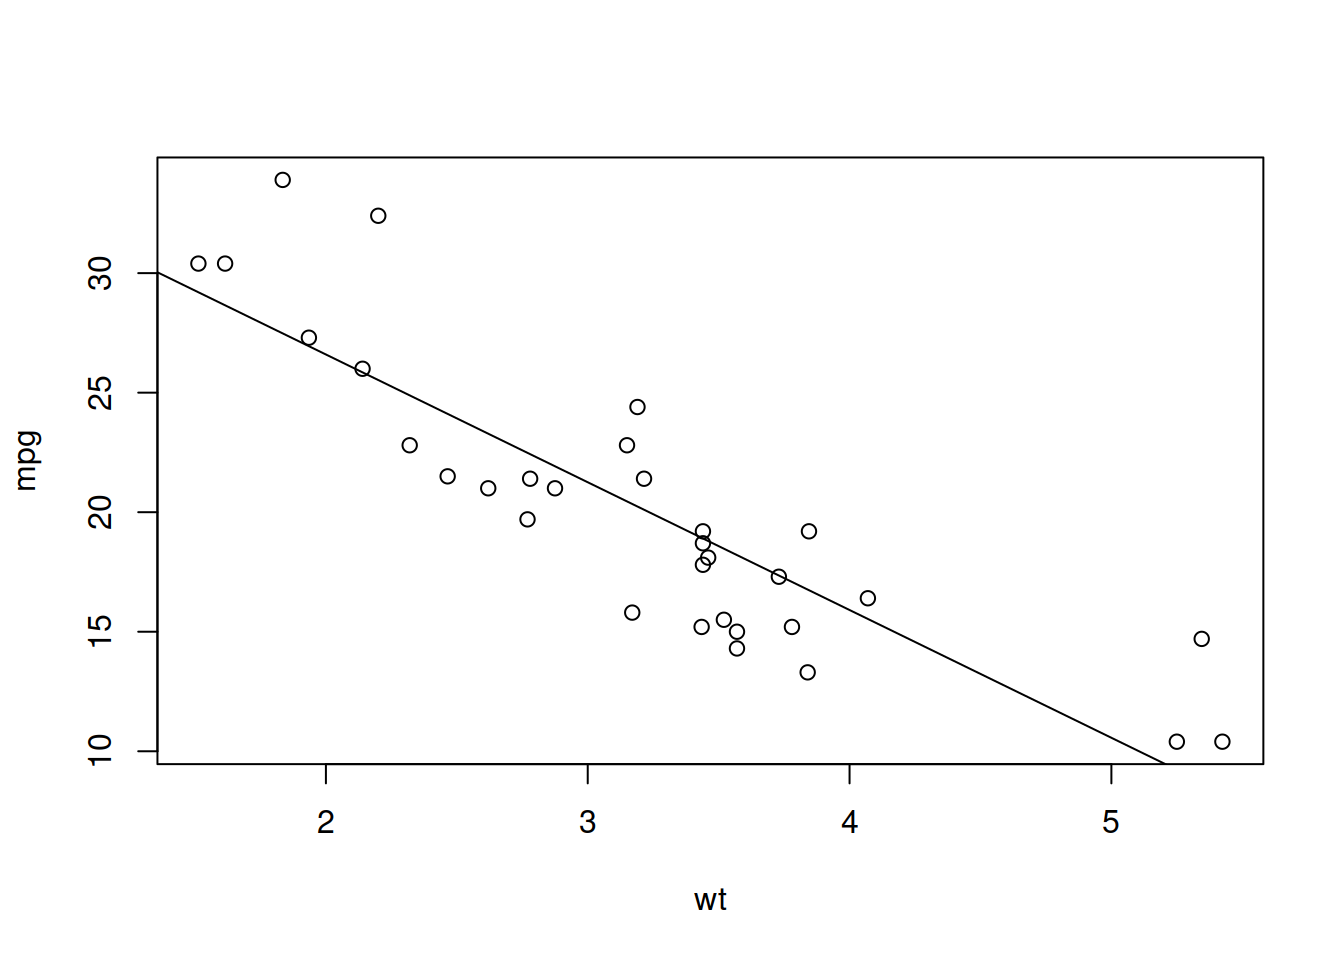
\includegraphics{L01-Intro_PicturingGraphs_files/figure-pdf/unnamed-chunk-4-1.pdf}

}

\end{figure}

Compare this to the output of \texttt{table(mtcars\$am)}:

\begin{Shaded}
\begin{Highlighting}[]
\FunctionTok{table}\NormalTok{(mtcars}\SpecialCharTok{$}\NormalTok{am)}
\end{Highlighting}
\end{Shaded}

\begin{verbatim}

 0  1 
19 13 
\end{verbatim}

Bar charts are primarily used to compare categories. The most common use
of a bar chart is to count the number of observations in each category,
and create a bar with a corresponding height. In this example, we see,
automatic and manual transmissions, with automatic labelled as zero and
manual labelled as one. We can see that approximately 22 cars are
automatic and 13 cars are manual. Unlike a pie chart, we can read these
numbers off of the plot and it's easy to compare these two categories.

The code required to create the bar chart can be shown by clicking the
``\textgreater Code'' icon. The data set is built into our so we don't
need to load anything to put this data. We do need to load in the
\texttt{ggplot} library, though. In my lecture notes, you'll see lots of
code that looks like this, but you will not be tested on your ability to
re-create this code. For those interested, here's a quick breakdown of
the functions I used:

\begin{itemize}
\tightlist
\item
  The ggplot function tells R what data we will be using.
\item
  The \texttt{aes()} function sets up the plot ``aesthetics'', such as
  what variable goes on the x-axis, what variable goes on the y-axis,
  what variable is assigned to a colour, what variable determines the
  shapes of points, etc.
\item
  \texttt{geom\_bar()} actually draws the bar plot using the data set
  that \texttt{ggplot()} set up and the aesthetics, that \texttt{aes()}
  set up.

  \begin{itemize}
  \tightlist
  \item
    Try running the code without this line and see what
    happens!\footnote{It will still create a plot with the correct x and
      y axes, but won't draw the bars.}
  \end{itemize}
\item
  The \texttt{labs()} function simply adds \texttt{lab}els to the plot
  to make it look nicer.
\end{itemize}

\textbf{Exercises}

The following exercises are based on the exercises in Chapter 1 of Baldi
\& Moore, 4th ed.

\begin{enumerate}
\def\labelenumi{\arabic{enumi}.}
\tightlist
\item
  Children's food choices. Does the presence of popular cartoon
  characters on food packages influence children's food choices? A study
  asked 40 young children (ages four to six) to taste two small pieces
  of Graham Crackers coming from a package with and a package without a
  popular cartoon character, and to indicate whether the two foods
  tasted the same or one tasted better. Unknown to the children, the
  crackers were the same both times. Here are the findings:
\end{enumerate}

\begin{longtable}[]{@{}lll@{}}
\toprule\noalign{}
Taste Preference & Number of Children & Percent \\
\midrule\noalign{}
\endhead
\bottomrule\noalign{}
\endlastfoot
Tastes better without character & 3 & \\
Taste the same & 15 & \\
Tastes better with character & 22 & \\
\end{longtable}

\begin{enumerate}
\def\labelenumi{\alph{enumi}.}
\tightlist
\item
  Identify the individuals and the variable or variables in the study.
\item
  Present these data in a well-labeled bar graph.
\item
  Would it also be correct to present these data in a single pie chart?
  Explain your reasoning.
\item
  What do the data suggest about the influence of cartoon characters on
  Graham Cracker preference in young children
\end{enumerate}

\begin{enumerate}
\def\labelenumi{\arabic{enumi}.}
\setcounter{enumi}{1}
\tightlist
\item
  The study in Exercise 1 also asked the 40 children to taste small
  pieces of gummy fruit snacks and baby carrots presented in packages
  with and in packages without a popular cartoon character. For each
  food type, the children indicated which of the two options they would
  prefer to eat for a snack. (Note that this is a different question
  from the one asked in Exercise 1) The number and percent of children
  choosing the version with a cartoon on the package are displayed in
  the following table:
\end{enumerate}

\begin{longtable}[]{@{}
  >{\raggedright\arraybackslash}p{(\columnwidth - 4\tabcolsep) * \real{0.3333}}
  >{\raggedright\arraybackslash}p{(\columnwidth - 4\tabcolsep) * \real{0.3333}}
  >{\raggedright\arraybackslash}p{(\columnwidth - 4\tabcolsep) * \real{0.3333}}@{}}
\toprule\noalign{}
\begin{minipage}[b]{\linewidth}\raggedright
Food Item
\end{minipage} & \begin{minipage}[b]{\linewidth}\raggedright
Number of children choosing the cartooon version
\end{minipage} & \begin{minipage}[b]{\linewidth}\raggedright
Percent choosing the cartoon
\end{minipage} \\
\midrule\noalign{}
\endhead
\bottomrule\noalign{}
\endlastfoot
Graham Crackers & 35 & \\
Gummy and fruit snacks & 34 & \\
Baby carrots & 29 & \\
\end{longtable}

\begin{enumerate}
\def\labelenumi{\alph{enumi}.}
\tightlist
\item
  Identify the individuals and the variable or variables in the study.
\item
  Make a well-labeled bar graph of the data.
\item
  Would it be correct to present these data in a single pie chart?
  Explain your reasoning.
\item
  What can you conclude from these findings?
\end{enumerate}

\hypertarget{ordered-and-unordered}{%
\subsection{Ordered and Unordered}\label{ordered-and-unordered}}

Whether the categorical variable is ordered or unordered affects the way
we make the plot:

\begin{itemize}
\tightlist
\item
  Ordered: put the bars in order
\item
  Unordered: put it in an arbitrary order

  \begin{itemize}
  \tightlist
  \item
    Alternative: order according to largest to smallest.
  \end{itemize}
\end{itemize}

\begin{Shaded}
\begin{Highlighting}[]
\FunctionTok{library}\NormalTok{(palmerpenguins)}
\FunctionTok{ggplot}\NormalTok{(penguins) }\SpecialCharTok{+}
    \FunctionTok{aes}\NormalTok{(}\AttributeTok{x =}\NormalTok{ species) }\SpecialCharTok{+}
    \FunctionTok{geom\_bar}\NormalTok{() }\SpecialCharTok{+}
    \FunctionTok{labs}\NormalTok{(}\AttributeTok{x =} \StringTok{"Species"}\NormalTok{, }\AttributeTok{y =} \StringTok{"Count"}\NormalTok{,}
        \AttributeTok{title =} \StringTok{"Unordered Categories"}\NormalTok{)}
\end{Highlighting}
\end{Shaded}

\begin{figure}[H]

{\centering \includegraphics{L01-Intro_PicturingGraphs_files/figure-pdf/unnamed-chunk-6-1.pdf}

}

\end{figure}

\begin{Shaded}
\begin{Highlighting}[]
\FunctionTok{library}\NormalTok{(forcats) }\CommentTok{\# For rearranging "factors", aka. categorical variables}
\FunctionTok{ggplot}\NormalTok{(penguins) }\SpecialCharTok{+}
    \FunctionTok{aes}\NormalTok{(}\AttributeTok{x =} \FunctionTok{fct\_infreq}\NormalTok{(species)) }\SpecialCharTok{+}
    \FunctionTok{geom\_bar}\NormalTok{() }\SpecialCharTok{+}
    \FunctionTok{labs}\NormalTok{(}\AttributeTok{x =} \StringTok{"Species"}\NormalTok{, }\AttributeTok{y =} \StringTok{"Count"}\NormalTok{,}
        \AttributeTok{title =} \StringTok{"Unordered Categories, Ordered by Count"}\NormalTok{)}
\end{Highlighting}
\end{Shaded}

\begin{figure}[H]

{\centering \includegraphics{L01-Intro_PicturingGraphs_files/figure-pdf/unnamed-chunk-7-1.pdf}

}

\end{figure}

The bar chart is the de-facto standard for categorical variables,
whether binary or otherwise. For quantitative, variables, we need other
options.

\hypertarget{quantitative-variables}{%
\subsection{Quantitative Variables}\label{quantitative-variables}}

Recall the distinction between discrete and continuous:

\begin{itemize}
\tightlist
\item
  Discrete (whole numbers)

  \begin{itemize}
  \tightlist
  \item
    Ex. Number of students in a classroom.
  \end{itemize}
\item
  Continuous (could be measured with more precision)

  \begin{itemize}
  \tightlist
  \item
    Ex. height
  \end{itemize}
\end{itemize}

\begin{tcolorbox}[enhanced jigsaw, toptitle=1mm, colbacktitle=quarto-callout-warning-color!10!white, breakable, leftrule=.75mm, left=2mm, opacityback=0, colframe=quarto-callout-warning-color-frame, rightrule=.15mm, toprule=.15mm, bottomtitle=1mm, titlerule=0mm, title=\textcolor{quarto-callout-warning-color}{\faExclamationTriangle}\hspace{0.5em}{Grey Area}, arc=.35mm, colback=white, bottomrule=.15mm, opacitybacktitle=0.6, coltitle=black]

What type of variable is ``dose level'', defined as either no dose, half
dose, or full dose? They aren't whole numbers, but we can't measure them
with greater precision!

\end{tcolorbox}

Quantitative variables are split into discrete and continuous variables.
Discrete variables are generally represented by whole numbers, for
example, the number of students in a given classroom.

In contrast, continuous numbers could be anything! I like to think of
them as numbers that could've been measured with more precision if we
had better tools. For example, peoples Heights could be measured to
infinite precision if we had perfect tools, whereas we don't need better
tools to measure the number of children and family more precisely.

Of course, as with all things, there is a gray area here. Many studies
will choose to give their subjects either no dose, a half dose or a full
dose. These are obviously numbers and it is very likely that the
response for a 0.75 dose is somewhere in between the half dose and the
full dose. However, we chose these numbers and thus there are only three
possible numbers. No amount of measuring is going to give us something
other than a half dose (any deviation in administration of the dose can
hopefully be ignored for the purpose of the study). In the definitions
we've used it is neither a whole number, nor cannot be measured with
higher precision. For the purposes of visualization, we might actually
want to use a bar chart as if this were a categorical variable. If the
dose had more categories and we expected the response to have a smooth
trend across different dose levels, then we might use visualizations
meant for discrete data. If the dose could have been any number between
zero and one then we might use visualization meant for continuous data.

\hypertarget{plotting-quantitative-variables}{%
\subsection{Plotting Quantitative
Variables}\label{plotting-quantitative-variables}}

Here are the lengths of sharks:

\begin{verbatim}
 9.4 12.1 12.2 12.3 12.4 12.6 13.2 13.2 13.2 13.2 13.5
13.6 13.6 13.8 14.3 14.6 14.7 14.9 15.2 15.3 15.7 15.7
15.8 15.8 16.1 16.2 16.2 16.4 16.4 16.6 16.7 16.8 16.8
17.6 17.8 17.8 18.2 18.3 18.6 18.7 18.7 19.1 19.7 22.8
\end{verbatim}

\begin{itemize}
\tightlist
\item
  We could have measured more precisely!

  \begin{itemize}
  \tightlist
  \item
    This is a continuous variable.
  \end{itemize}
\item
  Can't just draw a bar chart with all sharks that were 9.4, all that
  were 12.1, \ldots{}
\end{itemize}

How many we display this collection of shark lengths? It is clear that
there are many different values that we could've gotten for the length
and so we might not want to use something like a bar chart. Let's try it
anyway.

\hypertarget{quantitative-variables-as-a-bar-chart}{%
\subsection{Quantitative Variables as a Bar
Chart}\label{quantitative-variables-as-a-bar-chart}}

\begin{Shaded}
\begin{Highlighting}[]
\FunctionTok{library}\NormalTok{(ggplot2)}
\FunctionTok{theme\_set}\NormalTok{(}\FunctionTok{theme\_bw}\NormalTok{())}
\NormalTok{sharks }\OtherTok{\textless{}{-}}  \FunctionTok{c}\NormalTok{(}\FloatTok{9.4}\NormalTok{, }\FloatTok{12.1}\NormalTok{, }\FloatTok{12.2}\NormalTok{, }\FloatTok{12.3}\NormalTok{, }\FloatTok{12.4}\NormalTok{, }\FloatTok{12.6}\NormalTok{, }\FloatTok{13.2}\NormalTok{, }\FloatTok{13.2}\NormalTok{, }\FloatTok{13.2}\NormalTok{, }\FloatTok{13.2}\NormalTok{, }\FloatTok{13.5}\NormalTok{,}
\FloatTok{13.6}\NormalTok{, }\FloatTok{13.6}\NormalTok{, }\FloatTok{13.8}\NormalTok{, }\FloatTok{14.3}\NormalTok{, }\FloatTok{14.6}\NormalTok{, }\FloatTok{14.7}\NormalTok{, }\FloatTok{14.9}\NormalTok{, }\FloatTok{15.2}\NormalTok{, }\FloatTok{15.3}\NormalTok{, }\FloatTok{15.7}\NormalTok{, }\FloatTok{15.7}\NormalTok{,}
\FloatTok{15.8}\NormalTok{, }\FloatTok{15.8}\NormalTok{, }\FloatTok{16.1}\NormalTok{, }\FloatTok{16.2}\NormalTok{, }\FloatTok{16.2}\NormalTok{, }\FloatTok{16.4}\NormalTok{, }\FloatTok{16.4}\NormalTok{, }\FloatTok{16.6}\NormalTok{, }\FloatTok{16.7}\NormalTok{, }\FloatTok{16.8}\NormalTok{, }\FloatTok{16.8}\NormalTok{,}
\FloatTok{17.6}\NormalTok{, }\FloatTok{17.8}\NormalTok{, }\FloatTok{17.8}\NormalTok{, }\FloatTok{18.2}\NormalTok{, }\FloatTok{18.3}\NormalTok{, }\FloatTok{18.6}\NormalTok{, }\FloatTok{18.7}\NormalTok{, }\FloatTok{18.7}\NormalTok{, }\FloatTok{19.1}\NormalTok{, }\FloatTok{19.7}\NormalTok{, }\FloatTok{22.8}\NormalTok{)}

\FunctionTok{ggplot}\NormalTok{() }\SpecialCharTok{+} \FunctionTok{aes}\NormalTok{(}\AttributeTok{x =}\NormalTok{ sharks) }\SpecialCharTok{+} \FunctionTok{geom\_bar}\NormalTok{()}
\end{Highlighting}
\end{Shaded}

\begin{figure}[H]

{\centering \includegraphics{L01-Intro_PicturingGraphs_files/figure-pdf/unnamed-chunk-8-1.pdf}

}

\end{figure}

This plot demonstrates why bar chart isn't appropriate for these data.
We can see that each data point essentially gets its own bar, and so the
heights are no longer meaningful. The exception is that these data are
rounded to one decimal place, and so some lengths end up in the same
bar. Knowing that some of our data are rounded to the same value is not
necessarily meaningful for any analyses that we might want to do.
Instead, we would like a chart that shows us where most of the data are,
and whether or not they are clear patterns in these data.

\hypertarget{histograms-put-observations-into-bins}{%
\subsection{Histograms: Put observations into
bins}\label{histograms-put-observations-into-bins}}

The steps in building a histogram:

\begin{enumerate}
\def\labelenumi{\arabic{enumi}.}
\tightlist
\item
  Choose the bins.

  \begin{itemize}
  \tightlist
  \item
    e.g.~(0,10{]}, (10,20{]}, (20, 30{]}, etc.

    \begin{itemize}
    \tightlist
    \item
      The notation (a, b{]} means that ``a'' is \emph{not} included in
      the interval, but ``b'' is. We have no sharks that have a length
      of 0, but a shark with a recorded length of exactly 10 would be in
      the first bin, labelled (0, 10{]}, not the second bin that is
      labelled (10, 20{]}.
    \end{itemize}
  \end{itemize}
\item
  Count the number of obs. in each bin.
\item
  Draw a bar chart as if the bins are categories.

  \begin{itemize}
  \tightlist
  \item
    Bars should touch since there's nothing in between.
  \end{itemize}
\end{enumerate}

\begin{Shaded}
\begin{Highlighting}[]
\DocumentationTok{\#\# Note that I\textquotesingle{}ve manually chosen the bin widths and centers.}
\FunctionTok{ggplot}\NormalTok{() }\SpecialCharTok{+} 
    \FunctionTok{aes}\NormalTok{(}\AttributeTok{x =}\NormalTok{ sharks) }\SpecialCharTok{+}
    \FunctionTok{geom\_histogram}\NormalTok{(}\AttributeTok{binwidth=}\DecValTok{2}\NormalTok{, }
        \AttributeTok{center =} \DecValTok{0}\NormalTok{, }\CommentTok{\# Only need to specify the center of one bin}
        \AttributeTok{colour =} \StringTok{"black"}\NormalTok{, }\AttributeTok{fill =} \StringTok{"lightgrey"}\NormalTok{) }\SpecialCharTok{+}
    \FunctionTok{labs}\NormalTok{(}\AttributeTok{x =} \StringTok{"Shark Length"}\NormalTok{, }\AttributeTok{y =} \StringTok{"Count"}\NormalTok{)}
\end{Highlighting}
\end{Shaded}

\begin{figure}[H]

{\centering \includegraphics{L01-Intro_PicturingGraphs_files/figure-pdf/unnamed-chunk-9-1.pdf}

}

\end{figure}

In this histogram, the bins are (-1, 1{]}, (1,3{]}, (3,5{]}\ldots{}

Notice how the y-axis is still ``Counts'' (like a bar chart).

Most of the time we will probably want to use a histogram to display
quantitative, continuous data. A histogram is very much like putting
continuous numbers into discrete bins, and then showing it as a bar
chart. In this example, I chose bins from 1 to 3, then 3 to 5, then 5 to
7, and so on. For the bar on this histogram centred at a shark length of
12 we can see that there were five observations between 11 and 13. Note
that the definitions of bins has a round bracket on the left side and
the square bracket on the right side, this is to say that the left end
point \emph{is not} included but the right end point \emph{is} included.
This is just to account for cases where X may fall directly on the
border between two bins, and we have to choose which bin. The actual bin
we choose is arbitrary, kind of like driving in the left or the right.
You will not be tested on whether you can remember which endpoint is
inclusive.

From the plot, we can see that most of the sharks are around 16 feet in
length with sun going down to 10 feet and some as long as around 22
feet. The plot has a nice bell shape.

\hypertarget{histograms-bin-width-matters}{%
\subsection{Histograms: Bin Width
Matters!}\label{histograms-bin-width-matters}}

These histograms are showing the same data!

\begin{Shaded}
\begin{Highlighting}[]
\FunctionTok{ggplot}\NormalTok{() }\SpecialCharTok{+} 
    \FunctionTok{aes}\NormalTok{(}\AttributeTok{x =}\NormalTok{ sharks) }\SpecialCharTok{+}
    \FunctionTok{geom\_histogram}\NormalTok{(}\AttributeTok{binwidth=}\DecValTok{2}\NormalTok{, }
        \AttributeTok{center =} \DecValTok{0}\NormalTok{, }\CommentTok{\# Only need to specify the center of one bin}
        \AttributeTok{colour =} \StringTok{"black"}\NormalTok{, }\AttributeTok{fill =} \StringTok{"lightgrey"}\NormalTok{) }\SpecialCharTok{+}
    \FunctionTok{labs}\NormalTok{(}\AttributeTok{x =} \StringTok{"Shark Length"}\NormalTok{, }\AttributeTok{y =} \StringTok{"Count"}\NormalTok{)}
\end{Highlighting}
\end{Shaded}

\begin{figure}[H]

{\centering \includegraphics{L01-Intro_PicturingGraphs_files/figure-pdf/unnamed-chunk-10-1.pdf}

}

\end{figure}

\begin{Shaded}
\begin{Highlighting}[]
\FunctionTok{ggplot}\NormalTok{() }\SpecialCharTok{+} 
    \FunctionTok{aes}\NormalTok{(}\AttributeTok{x =}\NormalTok{ sharks) }\SpecialCharTok{+}
    \FunctionTok{geom\_histogram}\NormalTok{(}\AttributeTok{binwidth=}\FloatTok{1.5}\NormalTok{, }
        \AttributeTok{center =} \FloatTok{0.75}\NormalTok{, }\CommentTok{\# Only need to specify the center of one bin}
        \AttributeTok{colour =} \StringTok{"black"}\NormalTok{, }\AttributeTok{fill =} \StringTok{"lightgrey"}\NormalTok{) }\SpecialCharTok{+}
    \FunctionTok{labs}\NormalTok{(}\AttributeTok{x =} \StringTok{"Shark Length"}\NormalTok{, }\AttributeTok{y =} \StringTok{"Count"}\NormalTok{)}
\end{Highlighting}
\end{Shaded}

\begin{figure}[H]

{\centering \includegraphics{L01-Intro_PicturingGraphs_files/figure-pdf/unnamed-chunk-11-1.pdf}

}

\end{figure}

In the previous graph, it looked like the distribution of sharks
followed a nice bell-shaped curve. However, if we use bins that are 1.5
units wide we get a plot that looks fairly different. It still looks
like most sharks are around 16 feet and some go down to 10 and some go
as high is 22 or 23, But we see a large bar that covers 12 to 13.5.

With histograms the bins that you choose are extremely important. Most
software have default values that are generally reasonable, But it's
always always always worth investigating other bins.

A simple version of the plot can be made as follows, where
\texttt{ggplot} chooses the bins automatically. Note that this is rarely
desireable, and you should almost always choose the bins yourself.

\begin{Shaded}
\begin{Highlighting}[]
\FunctionTok{ggplot}\NormalTok{() }\SpecialCharTok{+} 
    \FunctionTok{aes}\NormalTok{(}\AttributeTok{x =}\NormalTok{ sharks) }\SpecialCharTok{+}
    \FunctionTok{geom\_histogram}\NormalTok{()}
\end{Highlighting}
\end{Shaded}

\begin{figure}[H]

{\centering \includegraphics{L01-Intro_PicturingGraphs_files/figure-pdf/unnamed-chunk-12-1.pdf}

}

\end{figure}

Below is an app to visualize the difference that the binwidth can make!

\begin{Shaded}
\begin{Highlighting}[]
\NormalTok{shiny}\SpecialCharTok{::}\FunctionTok{runGitHub}\NormalTok{(}\AttributeTok{repo =} \StringTok{"DBecker7/DB7\_TeachingApps"}\NormalTok{, }
    \AttributeTok{subdir =} \StringTok{"Apps/DensHist"}\NormalTok{)}
\end{Highlighting}
\end{Shaded}

\hypertarget{describing-distributions}{%
\subsection{Describing Distributions}\label{describing-distributions}}

When you're asked to comment on a histogram, always mention the
following:

\begin{itemize}
\tightlist
\item
  \textbf{Shape}: \textbf{Unimodal}/\textbf{bimodal} and
  \textbf{skewness}

  \begin{itemize}
  \tightlist
  \item
    Skewness: put a glob of peanut butter on toast, ``skew'' it to one
    side.
  \end{itemize}
\item
  \textbf{Center}: midpoint (\textbf{mean}/\textbf{median})

  \begin{itemize}
  \tightlist
  \item
    \textbf{Mode} depends on the bin!
  \item
    Skewness shows up in the relation between mean and median: ``Mean
    less (than median) means left (skew).''
  \end{itemize}
\item
  \textbf{Spread}: the \textbf{range}/\textbf{variance}/\textbf{IQR}

  \begin{itemize}
  \tightlist
  \item
    More on IQR later!
  \end{itemize}
\item
  \textbf{Outliers}: points that don't fit the shape

  \begin{itemize}
  \tightlist
  \item
    More on outliers when we cover IQR!
  \end{itemize}
\end{itemize}

There are many shapes that a histogram can show. A distribution can be
skewed (or ``heavy-tailed''), which means that it looks like a bell
curve but one side has a longer/thicker tail. We also want to know about
several measures of the center of the distribution, as well as how
spread out it is. Outliers are also something interesting to note;
outliers are something that are \emph{not} part of the shape (so you
wouldn't consider them when evaluating the skewness of a distribution).

Try drawing out each of these shapes/patterns!

\hypertarget{example-what-is-the-shape}{%
\subsection{Example: What is the
Shape?}\label{example-what-is-the-shape}}

\includegraphics{L01-Intro_PicturingGraphs_files/figure-pdf/unnamed-chunk-14-1.pdf}

This represents a \textbf{bimodal} distribution because it has two peaks
(the word ``mode'' can refer to the category with the most observations,
but it can also refer to the top of a peak). This would be described as
a bimodal distribution with centres around 190 and 215, ranges around
195 to 205 and 205 to 235, with both peaks being symmetric and without
any outliers.

\hypertarget{example-what-is-the-shape-1}{%
\subsection{Example: What is the
Shape?}\label{example-what-is-the-shape-1}}

\includegraphics{L01-Intro_PicturingGraphs_files/figure-pdf/unnamed-chunk-15-1.pdf}

This is the classic sort of gotcha question that I like to use. This is
actually a bar chart that I modified so that the bars have no space
in-between - the x-labels are categories, not ranges! It may look
somewhat symmetric and unimodal without any outliers, but the x-labels
are out of order. These numbers are just numerical encodings of species
names - 1 refers to Adelie penguins, 2 refers to Chinstrap, and 3 refers
to Gentoo. These numbers were applied alphabetically because there isn't
really a logical way to order these species: they're unordered
categories!

So, basically, it does not make sense to talk about shape in a bar graph
where the labels could have been put in any order!

\hypertarget{purely-pedagogical-stem-and-leaf-plots.}{%
\subsection{Purely Pedagogical: Stem-and-Leaf
plots.}\label{purely-pedagogical-stem-and-leaf-plots.}}

Consider the data

\begin{verbatim}
12, 43, 12, 32, 53, 66, 78, 25, 36, 12, 26,
34, 98, 39, 44, 23, 15, 67, 1,  4,  54, 21
\end{verbatim}

\textbf{Stem-and-Leaf}

\begin{verbatim}
0  | 14
10 | 2225
20 | 1356
30 | 2469
40 | 34
50 | 34
60 | 67
70 | 8
80 |
90 | 8
\end{verbatim}

\textbf{Sideways Histogram}

\begin{Shaded}
\begin{Highlighting}[]
\NormalTok{mydata }\OtherTok{\textless{}{-}} \FunctionTok{c}\NormalTok{(}\DecValTok{12}\NormalTok{, }\DecValTok{43}\NormalTok{, }\DecValTok{12}\NormalTok{, }\DecValTok{32}\NormalTok{, }\DecValTok{53}\NormalTok{, }\DecValTok{66}\NormalTok{, }\DecValTok{78}\NormalTok{, }\DecValTok{25}\NormalTok{, }\DecValTok{36}\NormalTok{, }\DecValTok{12}\NormalTok{, }\DecValTok{26}\NormalTok{,}
    \DecValTok{34}\NormalTok{, }\DecValTok{98}\NormalTok{, }\DecValTok{39}\NormalTok{, }\DecValTok{44}\NormalTok{, }\DecValTok{23}\NormalTok{, }\DecValTok{15}\NormalTok{, }\DecValTok{67}\NormalTok{, }\DecValTok{1}\NormalTok{,  }\DecValTok{4}\NormalTok{,  }\DecValTok{54}\NormalTok{, }\DecValTok{21}\NormalTok{)}

\FunctionTok{ggplot}\NormalTok{() }\SpecialCharTok{+} \FunctionTok{theme\_minimal}\NormalTok{() }\SpecialCharTok{+}
    \FunctionTok{aes}\NormalTok{(}\AttributeTok{x =}\NormalTok{ mydata) }\SpecialCharTok{+}
    \FunctionTok{geom\_histogram}\NormalTok{(}\AttributeTok{binwidth =} \DecValTok{10}\NormalTok{, }\AttributeTok{center =} \DecValTok{5}\NormalTok{,}
        \AttributeTok{fill =} \StringTok{"lightgrey"}\NormalTok{, }\AttributeTok{colour =} \StringTok{"black"}\NormalTok{) }\SpecialCharTok{+}
    \FunctionTok{scale\_x\_continuous}\NormalTok{(}\AttributeTok{breaks =}\NormalTok{ (}\DecValTok{0}\SpecialCharTok{:}\DecValTok{10}\NormalTok{)}\SpecialCharTok{*}\DecValTok{10}\NormalTok{, }\AttributeTok{trans =} \StringTok{"reverse"}\NormalTok{, }\AttributeTok{expand =} \FunctionTok{c}\NormalTok{(}\DecValTok{0}\NormalTok{,}\DecValTok{0}\NormalTok{)) }\SpecialCharTok{+}
    \FunctionTok{coord\_flip}\NormalTok{() }\SpecialCharTok{+} 
    \FunctionTok{labs}\NormalTok{(}\AttributeTok{x =} \StringTok{"Value"}\NormalTok{, }\AttributeTok{y =} \ConstantTok{NULL}\NormalTok{)}
\end{Highlighting}
\end{Shaded}

\begin{figure}[H]

{\centering \includegraphics{L01-Intro_PicturingGraphs_files/figure-pdf/unnamed-chunk-16-1.pdf}

}

\end{figure}

This visualization technique is shown purely for pedagogical reasons. A
stem and leaf plot is like a histogram where the bins are all powers of
10. It isisplayed using the stem, which is the first digit and the leaf
which is the second digit. For example, the number 78 has a 7 in the
tens place (and were using the tens place as the stem) and an 8 in the
ones place (and we using the ones place as the leaf). In the stem and
leaf plot, 78 goes on the stem labelled 70 and it gets a leaf of eight.
Going the other way, we can see a stem labelled 90 and a leaf labelled
eight which corresponds to the number 98. For the stem labelled zero we
have the numbers one and four, for the stem label 10 we have the numbers
12, 12, 12, and 15, and so on.

Essentially, this is just a histogram. We're instead of drawing a bar
that corresponds to the number of observations in that bin, we are just
listing the observations in that bin. Compare the stem and leaf plot to
the sideways histogram on the right: in the first bin from 0 to 10 (not
including 10) there are two numbers, one and four, and the length of the
bin is two. For the stem label 20, we have the numbers 21, 23, 25 and
26, and this is displayed as a bar with link for in the histogram.

The main reason for showing this visualization technique is that it can
be very useful for tests and quizzes, because it allows you to create a
histogram without software. It also allows easy computation of the
median since all of the leaves are in order. These are not used in
practice, because in practice, you will have software to create
histograms \emph{and} find the median!

Note that the shape of the distribution can be seen from the stem and
leaf plot. It is a unimodal distribution that is right skewed and likely
does not have an outlier (there is one point that appears to be separate
from the others, but this is most likely due to bin choice).

\hypertarget{summary}{%
\subsection{Summary}\label{summary}}

\begin{itemize}
\tightlist
\item
  \textbf{Individuals} are what we make measurements on

  \begin{itemize}
  \tightlist
  \item
    Can be pairs, dates, or people
  \end{itemize}
\item
  \textbf{Variables} are what we measure

  \begin{itemize}
  \tightlist
  \item
    Can be derived from other measurements
  \end{itemize}
\item
  You will not be asked to do anything with pie charts in this course.
\item
  \textbf{Bar charts} show counts of categories.

  \begin{itemize}
  \tightlist
  \item
    Can optionally sum to 1 (like a pie chart).
  \end{itemize}
\item
  \textbf{Histograms} are like bar charts for binned data.

  \begin{itemize}
  \tightlist
  \item
    \textbf{Bins matter}.
  \item
    Must interpret \textbf{shape}.
  \end{itemize}
\end{itemize}

\hypertarget{participation-questions}{%
\section{Participation Questions}\label{participation-questions}}

\hypertarget{q1}{%
\subsection{Q1}\label{q1}}

Which of the following visualizations would be \emph{least} appropriate
for \textbf{discrete} data?

\begin{enumerate}
\def\labelenumi{\arabic{enumi}.}
\tightlist
\item
  Bar Chart
\item
  Histogram
\item
  Pie Chart
\item
  Stem-and-Leaf plot
\end{enumerate}

\hypertarget{q2}{%
\subsection{Q2}\label{q2}}

\vspace{0.5cm}

What shape is the distribution on the right?

\begin{enumerate}
\def\labelenumi{\arabic{enumi}.}
\tightlist
\item
  Symmetric
\item
  Left Skewed
\item
  Right Skewed
\end{enumerate}

\includegraphics{L01-Intro_PicturingGraphs_files/figure-pdf/unnamed-chunk-17-1.pdf}

\hypertarget{q3}{%
\subsection{Q3}\label{q3}}

Age was collected as the number of days since birth. What kind of
variable is this?

\begin{enumerate}
\def\labelenumi{\arabic{enumi}.}
\tightlist
\item
  Ordered categorical
\item
  Unorded categorical
\item
  Discrete
\item
  Continuous
\end{enumerate}

\hypertarget{q4}{%
\subsection{Q4}\label{q4}}

Age was collected as 0-17, 18-25, 25-34, or 35+. What kind of variable
is this?

\begin{enumerate}
\def\labelenumi{\arabic{enumi}.}
\tightlist
\item
  Ordered categorical
\item
  Unorded categorical
\item
  Discrete
\item
  Continuous
\end{enumerate}

\hypertarget{q5}{%
\subsection{Q5}\label{q5}}

Age was collected as age in years, then rounded to the nearest 10. What
kind of variable is the rounded value of age?

\begin{enumerate}
\def\labelenumi{\arabic{enumi}.}
\tightlist
\item
  Ordered categorical
\item
  Unorded categorical
\item
  Discrete
\item
  Continuous
\end{enumerate}

\hypertarget{q6}{%
\subsection{Q6}\label{q6}}

\vspace{1cm}

Approximately what proportion of the data is larger than 0? Note that
there are 40 data points.

\begin{enumerate}
\def\labelenumi{\arabic{enumi}.}
\tightlist
\item
  50\%
\item
  25\%
\item
  75\%
\item
  100\%
\end{enumerate}

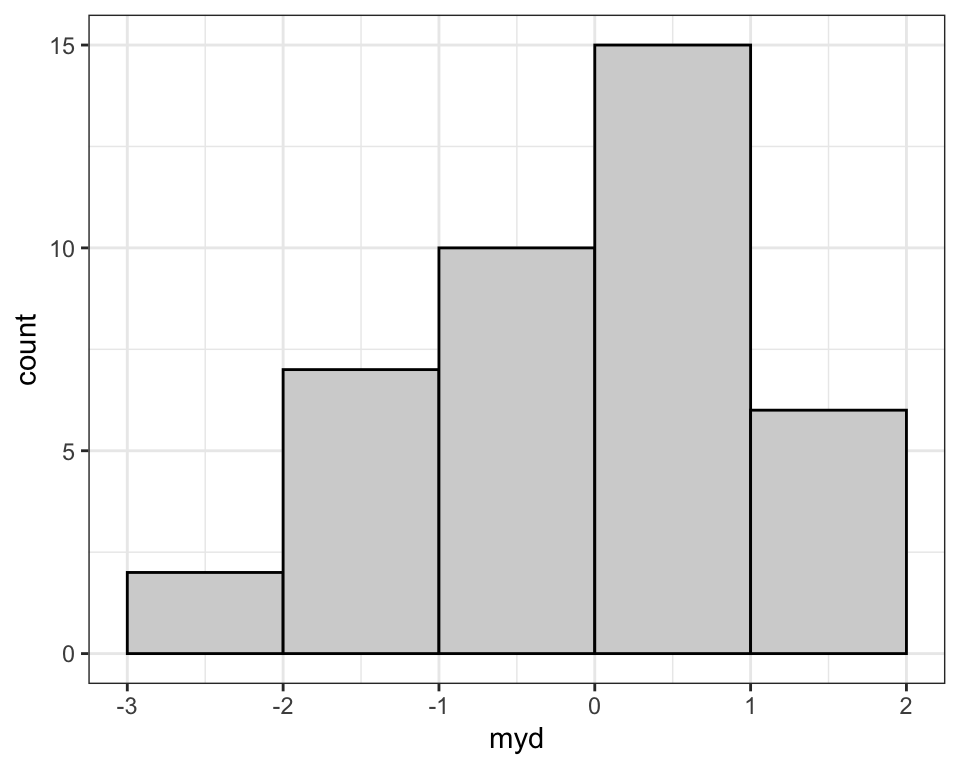
\includegraphics{L01-Intro_PicturingGraphs_files/figure-pdf/unnamed-chunk-18-1.pdf}

Answers: 334133

\textbf{Exercises}

\begin{enumerate}
\def\labelenumi{\arabic{enumi}.}
\tightlist
\item
  \textbf{Prescriptions of opioid pain relievers.} Opioid pain relievers
  are prescribed at a higher rate in the United States than in any other
  nation, even though abuse of these medications can result in addiction
  and fatal overdoses. The CDC examined opioid pain reliever
  prescriptions in each state to find out how variable prescription
  rates are across the nation. Here are the 2012 state prescription
  rates, in number of prescriptions per 100 people, listed in increasing
  order:
\end{enumerate}

\texttt{opiods\ \textless{}-\ c(52.0,\ 57.0,\ 59.5,\ 61.6,\ 62.9,\ 65.1,\ 66.5,\ 67.4,\ 67.9,\ 69.6,\ 70.8,\ 71.2,\ 71.7,\ 72.4,\ 72.7,\ 72.8,\ 73.8,\ 74.3,\ 74.3,\ 74.7,\ 76.1,\ 77.3,\ 77.5,\ 79.4,\ 82.0,\ 82.4,\ 85.1,\ 85.6,\ 85.8,\ 88.2,\ 89.2,\ 89.6,\ 90.7,\ 90.8,\ 93.8,\ 94.1,\ 94.8,\ 96.6,\ 100.1,\ 101.8,\ 107.0,\ 109.1,\ 115.8,\ 118.0,\ 120.3,\ 127.8,\ 128.4,\ 137.6,\ 142.8,\ 142.9)}

\begin{enumerate}
\def\labelenumi{\alph{enumi}.}
\tightlist
\item
  Make a histogram of the state opioid pain reliever prescription rates
  using classes of width 10 starting at 50.0 prescriptions per 100
  people. e.g.~(50, 60{]}. Do this by hand first, then using R.
\item
  Would you say that the distribution is single-peaked or
  multiple-peaked? Is it roughly symmetric or skewed?
\end{enumerate}

The Statistical Abstract of the United States, prepared by the Census
Bureau, provides the number of single-organ transplants for the year
2010, by organ. The following two exercises are based on this table:

\begin{longtable}[]{@{}ll@{}}
\toprule\noalign{}
Disease & Count \\
\midrule\noalign{}
\endhead
\bottomrule\noalign{}
\endlastfoot
Heart & 2,333 \\
Lung & 1,770 \\
Liver & 6,291 \\
Kidney & 16,898 \\
Pancreas & 350 \\
Intestine & 151 \\
\end{longtable}

\begin{enumerate}
\def\labelenumi{\arabic{enumi}.}
\setcounter{enumi}{1}
\tightlist
\item
  (1.14 in BM) The data on single-organ transplants can be displayed in
\end{enumerate}

\begin{enumerate}
\def\labelenumi{\alph{enumi}.}
\tightlist
\item
  a pie chart but not a bar graph.
\item
  a bar graph but not a pie chart.
\item
  either a pie chart or a bar graph.
\end{enumerate}

\begin{enumerate}
\def\labelenumi{\arabic{enumi}.}
\setcounter{enumi}{2}
\tightlist
\item
  (1.15 in BM) Kidney transplants represented what percent of single-
  organ transplants in 2010?
\end{enumerate}

\begin{enumerate}
\def\labelenumi{\alph{enumi}.}
\tightlist
\item
  Nearly 61\%.
\item
  One-sixth (nearly 17\%).
\item
  This percent cannot be calculated from the information provided in the
  table.
\end{enumerate}

See also:
\href{https://stats.libretexts.org/Bookshelves/Introductory_Statistics/Book\%3A_OpenIntro_Statistics_(Diez_et_al)./01\%3A_Introduction_to_Data/1.E\%3A_Introduction_to_Data_(Exercises)}{OpenIntro
Textbook} problems relating to visualizations that we have learned,
especially 1.30, 1.36, 1.37, 1.39, 1.40, 1.47.

\hypertarget{describing-distributions-with-numbers}{%
\chapter{Describing Distributions with
Numbers}\label{describing-distributions-with-numbers}}

\hypertarget{quantitative-variables-1}{%
\subsection{Quantitative Variables}\label{quantitative-variables-1}}

\hypertarget{parameters-versus-statistics}{%
\subsection{Parameters Versus
Statistics}\label{parameters-versus-statistics}}

\begin{itemize}
\tightlist
\item
  Numerical summaries are called parameters when they describe an entire
  population, and statistics when they describe a sample
\item
  Since we typically will not collect data on the entire population, we
  use (sample) statistics to make statements (with some uncertainty)
  about what the (population) parameter is.
\item
  Categorical variables are summarized by the count or proportion
  (percent) of the data in each category.
\item
  Quantitative variables are summarized by the centre and spread of the
  data
\end{itemize}

\hypertarget{parameters-versus-statistics-truth}{%
\subsection{\texorpdfstring{Parameters Versus Statistics:
``\,````Truth''``\,''}{Parameters Versus Statistics: ``\,``\,``Truth''\,``\,''}}\label{parameters-versus-statistics-truth}}

We assume there's some ``true'' population mean.

\begin{itemize}
\tightlist
\item
  This will change if, say, a new baby is born.
\end{itemize}

We cannot know the population parameter!

If we were able to measure the height of every Canadian at this very
instant, we would get one value. We can't do this though, so we collect
a sample instead. We try to collect the sample in such a way that we get
value close to the population parameter.

In this course, we make a big distinction between population parameter
and sample statistic. A sample statistic is something that we calculate
from a sample, where is the population? Parameter is the value that we
would get if we had the whole population.

Most of this course is centred around using the sample statistic to get
an idea of what the population parameter might be.

\hypertarget{measures-of-centre}{%
\subsection{Measures of Centre}\label{measures-of-centre}}

\hypertarget{the-centre}{%
\subsection{The Centre}\label{the-centre}}

The ``centre'' is a strange concept.

\begin{itemize}
\tightlist
\item
  Where are ``most'' of the data?
\item
  If we took an individual at random, what's the ``best guess'' of their
  height?
\end{itemize}

We want to \textbf{summarize} the data using a few words/numbers.

I prefer the second description here - if I were to make a prediction, I
want my predicted value to be close to the actual value. For example, I
might want to design something that fits the average person's height. I
must make a prediction about the height of the people that will use it.
My prediction is chosen to minimize how far off I would be, which means
that I want to be near the ``centre''.

\hypertarget{centre-1-the-median}{%
\subsection{Centre 1: The Median}\label{centre-1-the-median}}

The \textbf{median} (\(M\)) is the midpoint of a distribution: half the
observations are smaller and the other half are larger than it. To find
the median:

\begin{enumerate}
\def\labelenumi{\arabic{enumi}.}
\tightlist
\item
  Arrange all observations in order of size, from smallest to largest.
\item
  If the number of observations (\(n\)) is odd, the median \(M\) is the
  centre observation in the ordered list. Find the location of the
  median by counting \((n + 1)/2\) observations up from the smallest
  observation.
\item
  If n is even, the median \(M\) halfway between the two centre
  observations in the ordered list. The location of the median is again
  \((n + 1)/2\), counting from the smallest observation in the list.
\end{enumerate}

Basically, the median is the middle value. With odd \(n\), the middle
value is one of the observations, but when \(n\) is even we have to go
in between two values.

\hypertarget{example-1-odd-n}{%
\subsection{\texorpdfstring{Example 1: Odd
\(n\)}{Example 1: Odd n}}\label{example-1-odd-n}}

The distribution of needle lengths is how species of pine trees are
characterized. The following data are the lengths (in cm) of a sample of
15 needles taken at random from different parts of several Aleppo pine
trees (Southern California). What is the median length?

\begin{verbatim}
7.20 7.60  8.50  8.50  8.70  9.00  9.00 9.30
9.40 9.40 10.20 10.90 11.30 12.10 12.80
\end{verbatim}

\hypertarget{example-2-even-n}{%
\subsection{\texorpdfstring{Example 2: Even
\(n\)}{Example 2: Even n}}\label{example-2-even-n}}

We also have the lengths (in cm) of 18 needles from trees of the
noticeably different Torrey pine species. What is the median length for
these 18 pine needles? The ordered data are:

\begin{verbatim}
21.20 21.60 21.70 23.10 23.70 24.20 24.20 25.50 26.60
26.80 28.90 29.00 29.70 29.70 30.20 32.50 33.70 33.70
\end{verbatim}

\hypertarget{example-3-robustness}{%
\subsection{Example 3: Robustness}\label{example-3-robustness}}

\begin{verbatim}
Set 1: 1 2 3 4 5 6
Set 2: 1 1 1 6 6 6
Set 3: -2000 -1000 3 4 5000 60000000
\end{verbatim}

All three have the same median!

Do the ``centres'' make sense? Do they provide a good summary?

These three data sets demonstrate that the median only depends on the
middle two numbers when \(n\) is odd. For the first two data sets, the
median does seem to describe centre of the data well. The last data set
is a little bit different from the others and the median might not be
enough information.

\hypertarget{the-mean}{%
\subsection{The Mean}\label{the-mean}}

The mean is defined as:

\[
\bar x = \frac{1}{n}(x_1 + x_2 + ... + x_n)= \frac{1}{n}\sum_{i=1}^nx_i
\]

For example, the mean of (1, 2, 3, 4) is \[
\frac{1}{4}(1 + 2 + 3 + 4) = \frac{10}{4} = 2.5
\] (this also happens to be the median!)

This formula for the mean may look a little bit scary, but all it means
is that we add up all of the values that we have and divide by the
number of values.

Create a couple examples yourself and find the mean! If you create a
list of values, you can use R to check your work as follows:

\begin{Shaded}
\begin{Highlighting}[]
\NormalTok{my\_values }\OtherTok{\textless{}{-}} \FunctionTok{c}\NormalTok{(}\DecValTok{1}\NormalTok{, }\DecValTok{2}\NormalTok{, }\DecValTok{2}\NormalTok{, }\DecValTok{3}\NormalTok{, }\DecValTok{4}\NormalTok{, }\DecValTok{5}\NormalTok{, }\FloatTok{6.3212}\NormalTok{, }\DecValTok{3}\NormalTok{)}
\FunctionTok{mean}\NormalTok{(my\_values)}
\end{Highlighting}
\end{Shaded}

\begin{verbatim}
[1] 3.29015
\end{verbatim}

\begin{itemize}
\tightlist
\item
  The name ``\texttt{my\_values}'' could have been anything that is just
  letters, numbers, and underscores (no spaces, can't start with a
  number). It's just the name of an object in R.

  \begin{itemize}
  \tightlist
  \item
    An object is just a thing. You can put two things together, do a
    function of a thing, etc.
  \end{itemize}
\item
  \texttt{my\_values} is a \emph{vector}. That is, it's a collection of
  values.

  \begin{itemize}
  \tightlist
  \item
    We create it using the \texttt{c()} function, which means
    ``concatenate'', or ``put together''.
  \end{itemize}
\item
  The mean function takes a vector and calculates the mean for you.
\end{itemize}

To run this code, go to \url{wlu.syzygy.ca} and create a new R notebook.
Insert an ``R cell'', and copy/paste the code above into that cell.
Either hit the ``play'' button, or Alt+Enter (Option+Enter on a Mac).

\hypertarget{the-mean-is-not-robust}{%
\subsection{\texorpdfstring{The mean is \emph{not}
robust}{The mean is not robust}}\label{the-mean-is-not-robust}}

Consider the following sets of data:

\begin{verbatim}
Set 1: 1, 2, 3, 4, 5, 6
Set 2: 1, 2, 3, 4, 5, 60
\end{verbatim}

\begin{itemize}
\tightlist
\item
  Both have the same median.
\item
  Mean of 3.5 and 12.5, respectively.
\end{itemize}

Which do you think is the correct measure of the centre?

Unlike the median, which only depends on the middle value, the mean uses
information from all of the values. This means that if there's an
outlier or a misrecorded point, the mean will reflect this. Sometimes
this is what we want and sometimes it is not.

A common example of when the mean is not what we want is income. The
lowest possible income is zero, but there is no maximum income, so
incomes tend to be right skewed. The right skew affects the mean a lot
more than that affects the median, and so, in this case the median is a
better measure of the most common levels of income.

\hypertarget{mean-and-median-vs.-skew-mean-less-means-left}{%
\subsection{Mean and Median vs.~Skew: Mean less means
left}\label{mean-and-median-vs.-skew-mean-less-means-left}}

\begin{Shaded}
\begin{Highlighting}[]
\NormalTok{shiny}\SpecialCharTok{::}\FunctionTok{runGitHub}\NormalTok{(}\AttributeTok{repo =} \StringTok{"DBecker7/DB7\_TeachingApps"}\NormalTok{, }
    \AttributeTok{subdir =} \StringTok{"Apps/MeanLessMeansLeft"}\NormalTok{)}
\end{Highlighting}
\end{Shaded}

The app above will be used in class, so do not worry if you're unable to
run it. It demonstrates that when they mean is less than the median it
means it's left skewed. The reason for this is that the outliers to the
left affect the mean more than they affect the median.

\hypertarget{measures-of-spread}{%
\section{Measures of Spread}\label{measures-of-spread}}

\hypertarget{which-has-more-variance}{%
\subsection{Which has more variance?}\label{which-has-more-variance}}

\begin{verbatim}
Set 1: 1 1 1 5 5 5
Set 2: 1 2 3 3 4 5
Set 3: 1 3 3 3 3 5
\end{verbatim}

\begin{itemize}
\tightlist
\item
  All have the same \textbf{range} (max - min).
\end{itemize}

These three data sets all have the same mean and median, but just
looking at them shows that they are differnt collections of numbers. The
first said, only has two unique values put those values are relatively
far away from each other compared to the other sets. The second set is a
more even spread from one to five. The third set has for value is equal
to the mean and two values that may be outliers.

To me, the first set looks like it's the most variable because all of
the values are very far away from either the mean or the median. The
second set has a smaller variance, because there are values closer to
the mean. And the last set I expect to have the lowest variance, because
most values are actually equal to the mean.

The formula for the variance, which will introduce next, matches this
intuition. However, many students have different intuitions about which
has the most variance and those are valid as well but are harder to
quantify.

\hypertarget{measure-of-spread-the-variance}{%
\subsection{Measure of Spread: The
Variance}\label{measure-of-spread-the-variance}}

Consider set 1, which has a mean of 3:

\begin{verbatim}
1 1 1 5 5 5
\end{verbatim}

\begin{itemize}
\tightlist
\item
  The distances to the mean are all -2 or 2

  \begin{itemize}
  \tightlist
  \item
    If we found the mean, we'd get 0! We need to make sure they're all
    positive.
  \end{itemize}
\item
  Alternative 1: Absolute value. The average \emph{absolute} distance to
  the mean is 2.
\item
  Alternative 2: Squared value.

  \begin{itemize}
  \tightlist
  \item
    The \textbf{average squared distance to the mean} is 4

    \begin{itemize}
    \tightlist
    \item
      Important: This is not the actual variance calculation!
    \end{itemize}
  \end{itemize}
\end{itemize}

The \textbf{variance} is the average \emph{squared} distance to the
mean!

(We use squared because math - more on this later).

We are basically looking at the average deviation from the mean. We want
that deviation to be positive and there are several ways to do this. We
have settled on squaring the numbers for the same reason we drive on the
right side of the road: it's just convention. There are benefits to
using the absolute distance from the mean, but there are many
mathematical advantages to squaring the values first.

\hypertarget{variance-formula}{%
\subsection{Variance Formula}\label{variance-formula}}

\vspace{1.5cm}

\[
s^2 = \frac{1}{n-1}\sum_{i=1}^n(x_i - \bar x)^2
\]

We use \(n-1\) because of math reasons.

The easiest way to calculate this is to put it in a table:

\begin{longtable}[]{@{}llll@{}}
\toprule\noalign{}
\(i\) & \(x_i\) & \(x_i - \bar x\) & \((x_i - \bar x)^2\) \\
\midrule\noalign{}
\endhead
\bottomrule\noalign{}
\endlastfoot
1 & 1 & -2 & 4 \\
2 & 1 & -2 & 4 \\
3 & 1 & -2 & 4 \\
4 & 5 & 2 & 4 \\
5 & 5 & 2 & 4 \\
6 & 5 & 2 & 4 \\
\(\sum\) & 18 & 0 & 24 \\
\end{longtable}

The mean is 3, and the variance is 24/5 = 4.8.

In the table above, as before, the subscript \(i\) is just used to
denote different observations. For example \(x_1\) is the first
observation, \(x_2\) is the second observation in our data, and so on
(this ordering is arbitrary).

In order to calculate the variance, we must first know the mean, and so
it's convenient to put this at the bottom of the table. We then squared
the deviations from the mean and divided by \(n-1\). There are very good
technical reasons why we divide by (n-1) that we won't get into here.
Come to my office and chat if you'd like to know more, or just ask
ChatGPT!

\begin{tcolorbox}[enhanced jigsaw, toptitle=1mm, colbacktitle=quarto-callout-note-color!10!white, breakable, leftrule=.75mm, left=2mm, opacityback=0, colframe=quarto-callout-note-color-frame, rightrule=.15mm, toprule=.15mm, bottomtitle=1mm, titlerule=0mm, title=\textcolor{quarto-callout-note-color}{\faInfo}\hspace{0.5em}{\(n-1\) in the denominator}, arc=.35mm, colback=white, bottomrule=.15mm, opacitybacktitle=0.6, coltitle=black]

As a quick explanation for \(n-1\), consider the variance of a single
observation. It doesn't vary! There's not enough information to see how
much variance there is. There isn't enough \emph{information} in our
data. The \(n-1\) in the denominator enforces this - we can't calculate
the variance of one observation.

\end{tcolorbox}

Note that the variance can be calculated in R as follows:

\begin{Shaded}
\begin{Highlighting}[]
\NormalTok{my\_values }\OtherTok{\textless{}{-}} \FunctionTok{c}\NormalTok{(}\DecValTok{1}\NormalTok{, }\DecValTok{2}\NormalTok{, }\DecValTok{2}\NormalTok{, }\DecValTok{3}\NormalTok{, }\DecValTok{4}\NormalTok{, }\DecValTok{5}\NormalTok{, }\FloatTok{6.3212}\NormalTok{, }\DecValTok{3}\NormalTok{)}
\FunctionTok{var}\NormalTok{(my\_values)}
\end{Highlighting}
\end{Shaded}

\begin{verbatim}
[1] 3.050982
\end{verbatim}

\hypertarget{the-variance-and-the-standard-deviation}{%
\subsection{The Variance and the Standard
Deviation}\label{the-variance-and-the-standard-deviation}}

\[
s = \sqrt{\frac{1}{n-1}\sum_{i=1}^n(x - \bar x)^2}
\]

The \textbf{standard deviation} (or \textbf{sd}) is just the square root
of the variance.

\begin{itemize}
\tightlist
\item
  This makes it have the same units as the original data.
\end{itemize}

In addition, if we have two data sets and the variance of one is larger
than the other, then the standard deviation is also larger. They're the
same thing, just in different units!

I will often refer to one when I mean the other. When I'm comparing
standard deviations, I may call them variances because the same patterns
will be there.

Here's the R code:

\begin{Shaded}
\begin{Highlighting}[]
\FunctionTok{sd}\NormalTok{(my\_values)}
\end{Highlighting}
\end{Shaded}

\begin{verbatim}
[1] 1.746706
\end{verbatim}

\begin{Shaded}
\begin{Highlighting}[]
\FunctionTok{sd}\NormalTok{(my\_values)}\SpecialCharTok{\^{}}\DecValTok{2} \CommentTok{\# the sd is the square root of the variance}
\end{Highlighting}
\end{Shaded}

\begin{verbatim}
[1] 3.050982
\end{verbatim}

\hypertarget{exercise-variation-of-the-three-sets}{%
\subsection{Exercise: Variation of the three
sets}\label{exercise-variation-of-the-three-sets}}

\begin{verbatim}
Set 1: 1 1 1 5 5 5
Set 2: 1 2 3 3 4 5
Set 3: 1 3 3 3 3 5
\end{verbatim}

\begin{enumerate}
\def\labelenumi{\arabic{enumi}.}
\tightlist
\item
  Draw out bar plots.
\item
  Set up the table and find the variance.
\item
  Compare the standard deviations; make a conclusion.
\end{enumerate}

\begin{longtable}[]{@{}llll@{}}
\toprule\noalign{}
\(i\) & \(x_i\) & \(x_i - \bar x\) & \((x_i - \bar x)^2\) \\
\midrule\noalign{}
\endhead
\bottomrule\noalign{}
\endlastfoot
1 & & & \\
2 & & & \\
3 & & & \\
4 & & & \\
5 & & & \\
6 & & & \\
\(\sum\) & & & \\
\end{longtable}

Fill out the table above yourself!

\hypertarget{measure-of-spread-2-the-iqr}{%
\subsection{Measure of Spread 2: The
IQR}\label{measure-of-spread-2-the-iqr}}

The IQR is very closely related to the median. But first, we will learn
what quartiles are.

Consider the data:

\begin{verbatim}
1 2 3 4 5 6 7 8
\end{verbatim}

The median of these data is 5; 50\% of the data are to the left of this
point.

\begin{itemize}
\tightlist
\item
  ``Quartile'': Split the data into four.

  \begin{itemize}
  \tightlist
  \item
    Q1: 25\% of the data are to the left.
  \item
    Q2: 50\% of the data are to the left (the median).
  \item
    Q3: 75\% of the data are to the left.
  \end{itemize}
\end{itemize}

\hypertarget{finding-quartiles}{%
\subsection{Finding Quartiles}\label{finding-quartiles}}

\begin{verbatim}
1 2 3 4 5 6 7 8
\end{verbatim}

\begin{enumerate}
\def\labelenumi{\arabic{enumi}.}
\tightlist
\item
  Find the median

  \begin{itemize}
  \tightlist
  \item
    It's 4.5. Cool.
  \end{itemize}
\item
  Q1 is just half of 50\% - we're finding a median again!

  \begin{itemize}
  \tightlist
  \item
    Q1 is the median of everything to the left of the median.
  \item
    In this case, 1 2 3 4 are the numbers to the left of the median, and
    so Q1 is 2.5.
  \end{itemize}
\item
  By a similar argument, Q3 is 6.5.
\end{enumerate}

Q0 is where 0\% of the data are to the left. In other words, it's the
minimum value in the data! Similarly, Q4 is the maximum value in the
data.

\begin{tcolorbox}[enhanced jigsaw, toptitle=1mm, colbacktitle=quarto-callout-warning-color!10!white, breakable, leftrule=.75mm, left=2mm, opacityback=0, colframe=quarto-callout-warning-color-frame, rightrule=.15mm, toprule=.15mm, bottomtitle=1mm, titlerule=0mm, title=\textcolor{quarto-callout-warning-color}{\faExclamationTriangle}\hspace{0.5em}{Warning}, arc=.35mm, colback=white, bottomrule=.15mm, opacitybacktitle=0.6, coltitle=black]

The algorithm we just used for computing the quartiles is not the only
one! In R, there are \emph{NINE} different ways to calculate the
quartiles. You should stick to doing this by hand if you want to get the
WeBWork answers right.

\end{tcolorbox}

\hypertarget{the-five-number-summary}{%
\subsection{The five number summary}\label{the-five-number-summary}}

Let's use the folowing example:

\begin{verbatim}
1, 3, 3, 4, 5, 5, 5, 6, 7, 7, 8, 8, 9, 10, 10, 11, 12
\end{verbatim}

The quartiles give an excellent way to summarise data:

\begin{longtable}[]{@{}lllll@{}}
\toprule\noalign{}
Q0 (min) & Q1 & Q2 (median) & Q3 & Q4 (max) \\
\midrule\noalign{}
\endhead
\bottomrule\noalign{}
\endlastfoot
1 & 4.5 & 7 & 8.5 & 12 \\
\end{longtable}

The five number summary just shows all five of the quartiles. Note that
there are five quartiles, because zero is also one of them.

For practice, make sure you can calculate the median, and then the
median of all the values to the left of it!

\hypertarget{visualizing-the-five-number-summary-the-boxplot}{%
\subsection{Visualizing the five number summary: the
boxplot}\label{visualizing-the-five-number-summary-the-boxplot}}

\vspace{1cm}

The plot on the right shows the body masses for the Palmer Penguins.

\begin{itemize}
\tightlist
\item
  The lowest point is Q0
\item
  The left of the box is Q1
\item
  The thick line in the box is Q2 (the median)
\item
  The right of the box is Q3
\item
  The highest point is Q4
\end{itemize}

\begin{Shaded}
\begin{Highlighting}[]
\FunctionTok{library}\NormalTok{(ggplot2)}
\FunctionTok{library}\NormalTok{(palmerpenguins)}
\FunctionTok{theme\_set}\NormalTok{(}\FunctionTok{theme\_bw}\NormalTok{())}

\FunctionTok{ggplot}\NormalTok{(penguins) }\SpecialCharTok{+} 
    \FunctionTok{aes}\NormalTok{(}\AttributeTok{y =}\NormalTok{ body\_mass\_g) }\SpecialCharTok{+}
    \FunctionTok{geom\_boxplot}\NormalTok{() }\SpecialCharTok{+}
    \FunctionTok{labs}\NormalTok{(}\AttributeTok{y =} \StringTok{"Body Mass (g)"}\NormalTok{) }\SpecialCharTok{+}
    \FunctionTok{coord\_flip}\NormalTok{()}
\end{Highlighting}
\end{Shaded}

\begin{figure}[H]

{\centering \includegraphics{L02-Describing_Distributions_Numbers_files/figure-pdf/unnamed-chunk-5-1.pdf}

}

\end{figure}

\begin{Shaded}
\begin{Highlighting}[]
\FunctionTok{ggplot}\NormalTok{(penguins) }\SpecialCharTok{+} 
    \FunctionTok{aes}\NormalTok{(}\AttributeTok{x =}\NormalTok{ body\_mass\_g) }\SpecialCharTok{+}
    \FunctionTok{geom\_histogram}\NormalTok{(}\AttributeTok{colour =} \DecValTok{1}\NormalTok{, }\AttributeTok{fill =} \StringTok{"lightgrey"}\NormalTok{) }\SpecialCharTok{+}
    \FunctionTok{labs}\NormalTok{(}\AttributeTok{x =} \StringTok{"Body Mass (g)"}\NormalTok{)}
\end{Highlighting}
\end{Shaded}

\begin{figure}[H]

{\centering \includegraphics{L02-Describing_Distributions_Numbers_files/figure-pdf/unnamed-chunk-6-1.pdf}

}

\end{figure}

The boxplot and the histogram both demonstrate the right skew of the
data, but the boxplot is much more compact!

Take a moment to compare the two plots and make sure you can explain the
skewness. Remember that 25\% of the data are in each interval shown in
the box plot!

\hypertarget{measure-2-the-inter-quartile-range-iqr}{%
\subsection{Measure 2: The Inter-Quartile Range
(IQR)}\label{measure-2-the-inter-quartile-range-iqr}}

The IQR is defined as: Q3 - Q1.

\begin{itemize}
\tightlist
\item
  Same units as the original data
\item
  Robust to outliers (unlike the sd)!
\end{itemize}

This is the second measure of spread that we will learn. The IQR is
commonly used when we have highly skewed data or data with outliers. The
sd measures the average squared deviation from the mean, whereas the IQR
measures the middle 50\% of the data.

Notice how this is not centered on the median. Consider the following
data:

\begin{Shaded}
\begin{Highlighting}[]
\NormalTok{my\_values }\OtherTok{\textless{}{-}} \FunctionTok{c}\NormalTok{(}\DecValTok{1}\NormalTok{, }\DecValTok{1}\NormalTok{, }\DecValTok{1}\NormalTok{, }\DecValTok{2}\NormalTok{, }\DecValTok{2}\NormalTok{, }\DecValTok{2}\NormalTok{, }\DecValTok{2}\NormalTok{, }\DecValTok{3}\NormalTok{, }\DecValTok{3}\NormalTok{, }\DecValTok{3}\NormalTok{, }\DecValTok{3}\NormalTok{, }\DecValTok{3}\NormalTok{, }\DecValTok{4}\NormalTok{, }\DecValTok{4}\NormalTok{, }\DecValTok{4}\NormalTok{, }\DecValTok{5}\NormalTok{, }\DecValTok{6}\NormalTok{, }\DecValTok{7}\NormalTok{, }\DecValTok{8}\NormalTok{, }\DecValTok{10}\NormalTok{)}
\FunctionTok{length}\NormalTok{(my\_values)}
\end{Highlighting}
\end{Shaded}

\begin{verbatim}
[1] 20
\end{verbatim}

\begin{Shaded}
\begin{Highlighting}[]
\FunctionTok{hist}\NormalTok{(my\_values)}
\end{Highlighting}
\end{Shaded}

\begin{figure}[H]

{\centering \includegraphics{L02-Describing_Distributions_Numbers_files/figure-pdf/unnamed-chunk-7-1.pdf}

}

\end{figure}

The median of these should be at position
\((n+1)/2 = (20 + 1)/2 = 10.5\) (I used the \texttt{length()} function
in R to count the number of observations for me). This value is halfway
between 3 and 3, meaning it's 3. Q1 is the median of the first 10 data
points, which is at position 5.5, giving us a value of 2. Q3 is 5.5
positions from the end, which is 4.5. Thus the IQR is \(4.5 - 2 = 2.5\).

First, does this make sense to you? Does 2.5 sound like a reasonable
width for the middle 50\%?

Now consider that the distribution is clearly skewed to the right. This
affects the variance a lot, but the IQR would have been the same no
matter what the first 4 or last 4 values were.

\hypertarget{iqr-for-outliers}{%
\subsection{IQR for Outliers}\label{iqr-for-outliers}}

In this class, we use a rule of thumb for calculating outliers. Anything
that is\ldots{}

\begin{itemize}
\tightlist
\item
  Below the median minus 1.5*IQR, or
\item
  above the median plus 1.5*IQR
\end{itemize}

is considered an outlier.

This rule of thumb is not based on any mathematical derivations, it just
seems to work in most situations.

The idea is that the IQR gives a measure of spread, and the median gives
the measure of the centre, so anything too far from the centre is an
outlier. We use the spread to figure out how far away from the centre we
are willing to accept. This will show up several times in this course.
We've seen it in this example for the IQR and median because this is
simple and easy to interpret.

Most of the rest of this course will be spent looking at something
similar for the mean. We will still use this idea of the centre plus or
minus some measure of the spread, but will incorporate information about
the sample and assumptions about the population that allow us to make
much stronger conclusions beyond simply checking if something is an
outlier.

\hypertarget{summary-1}{%
\subsection{Summary}\label{summary-1}}

\begin{itemize}
\tightlist
\item
  The ``centre'' is trying to measure the most common value.

  \begin{itemize}
  \tightlist
  \item
    Often, this is our best \textbf{prediction}.
  \end{itemize}
\item
  The ``spread'' is trying to measure the scale, or variation.

  \begin{itemize}
  \tightlist
  \item
    Gives context to the centre.
  \end{itemize}
\item
  The mean and variance

  \begin{itemize}
  \tightlist
  \item
    Interpretations and formulas are important.
  \end{itemize}
\item
  The median and IQR

  \begin{itemize}
  \tightlist
  \item
    Calculations, interpretations, five-number-summary, outliers, and
    boxplots are all important.
  \end{itemize}
\end{itemize}

We saw the same thing a couple of times throughout this lesson. We saw
measures of centre that try to describe the middle of a distribution and
centres of spread that tell us how spread out the data are. The mean and
the sd are intrinsically linked, and the median and IQR are
intrinsically linked.

We also saw the rule-of-thumb to use IQR for finding outliers by using
the median plus-an-minus some number times the spread. You better
believe that this idea will show up again later in this course!

Boxplots are a visual representation of the five number summary. These
can be very small while still showing the shape of our data. However,
these only work for unimodal data - there isn't a good way to show a
bimodal distribution on a boxplot. Also, it is very easy to plot two
boxplots for two different data sets in order to compare the
distributions.

For assignments and exams, be ready to calculate any of these values and
compare the mean/median and sd/IQR. Also be ready to compare the five
number summary to a boxplot.

\textbf{Exercises}

\begin{enumerate}
\def\labelenumi{\arabic{enumi}.}
\tightlist
\item
  \textbf{Spider Silk.} Spider silk is the strongest known material,
  natural or man-made, on a weight basis. A study examined the
  mechanical properties of spider silk using 21 female golden orb
  weavers, Nephila clavipes. Here are data on silk yield stress, which
  represents the amount of force per unit area needed to reach permanent
  deformation of the silk strand. The data are expressed in megapascals
  (MPa):
\end{enumerate}

\begin{verbatim}
164.00 173.00 176.10 236.10 251.30 270.50 270.50
272.40 282.20 288.80 290.70 300.60 327.20 329.00
332.10 351.70 358.20 362.00 448.90 478.70 740.20
\end{verbatim}

\begin{enumerate}
\def\labelenumi{\alph{enumi}.}
\tightlist
\item
  Describe the shape, centre, and spread of the data using a histogram
  (code below).
\item
  Find the mean and median yield stress. Compare these two values.
  Referring to the histogram produced by the code below, what general
  fact does your comparison illustrate?
\item
  Re-run the code using different values of \texttt{breaks}. What do you
  see? (Note that this example uses base R rather than \texttt{ggplot2}
  because it has simpler code - \texttt{ggplot2} has more flexibility,
  but that flexibility isn't necessary here.)
\item
  Use the \texttt{boxplot()} function to create a boxplot (you do not
  need the \texttt{breaks=10} part of the code). Compare this to the
  histogram. Also comment on any points that stand out (when there are
  outliers, R shows \(Q2\pm 1.5IQR\) rather than Q0 and Q4).
\item
  Use the \(Q2\pm 1.5IQR\) formula by hand to find the outliers, and
  verify your calculations with the R plot.
\end{enumerate}

\begin{Shaded}
\begin{Highlighting}[]
\NormalTok{silk\_stress }\OtherTok{\textless{}{-}} \FunctionTok{c}\NormalTok{(}\FloatTok{164.00}\NormalTok{, }\FloatTok{173.00}\NormalTok{, }\FloatTok{176.10}\NormalTok{, }\FloatTok{236.10}\NormalTok{, }\FloatTok{251.30}\NormalTok{, }\FloatTok{270.50}\NormalTok{, }\FloatTok{270.50}\NormalTok{,}
    \FloatTok{272.40}\NormalTok{, }\FloatTok{282.20}\NormalTok{, }\FloatTok{288.80}\NormalTok{, }\FloatTok{290.70}\NormalTok{, }\FloatTok{300.60}\NormalTok{, }\FloatTok{327.20}\NormalTok{, }\FloatTok{329.00}\NormalTok{,}
    \FloatTok{332.10}\NormalTok{, }\FloatTok{351.70}\NormalTok{, }\FloatTok{358.20}\NormalTok{, }\FloatTok{362.00}\NormalTok{, }\FloatTok{448.90}\NormalTok{, }\FloatTok{478.70}\NormalTok{, }\FloatTok{740.20}\NormalTok{)}
\FunctionTok{hist}\NormalTok{(silk\_stress, }\AttributeTok{breaks =} \DecValTok{10}\NormalTok{)}
\end{Highlighting}
\end{Shaded}

\begin{figure}[H]

{\centering \includegraphics{L02-Describing_Distributions_Numbers_files/figure-pdf/unnamed-chunk-8-1.pdf}

}

\end{figure}

\begin{enumerate}
\def\labelenumi{\arabic{enumi}.}
\setcounter{enumi}{1}
\item
  \textbf{Deep-sea sediments.} Phytopigments are markers of the amount
  of organic matter that settles in sediments on the ocean floor.
  Phytopigment concentrations in deep-sea sediments collected worldwide
  showed a very strong right-skew. Of two summary statistics, 0.015 and
  0.009 gram per square meter of bottom surface, which one is the mean
  and which one is the median? Explain your reasoning.
\item
  \textbf{Glucose levels.} People with diabetes must monitor and control
  their blood glucose level. The goal is to maintain a ``fasting plasma
  glucose'' between approximately 90 and 130 milligrams per deciliter
  (mg/dl). The data tables below give the fasting plasma glucose levels
  for two groups of diabetics five months after they received either
  group instruction or individual instruction on glucose control.
\end{enumerate}

I provide the data as vectors in R, but you don't need R for this
question (it's good practice to do it both ways).

\begin{Shaded}
\begin{Highlighting}[]
\NormalTok{group }\OtherTok{\textless{}{-}} \FunctionTok{c}\NormalTok{(}\FloatTok{78.00}\NormalTok{, }\FloatTok{95.00}\NormalTok{, }\FloatTok{96.00}\NormalTok{, }\FloatTok{103.00}\NormalTok{, }\FloatTok{112.00}\NormalTok{, }\FloatTok{134.00}\NormalTok{, }\FloatTok{141.00}\NormalTok{, }\FloatTok{145.00}\NormalTok{, }\FloatTok{147.00}\NormalTok{,}
    \FloatTok{148.00}\NormalTok{, }\FloatTok{153.00}\NormalTok{, }\FloatTok{158.00}\NormalTok{, }\FloatTok{172.00}\NormalTok{, }\FloatTok{172.00}\NormalTok{, }\FloatTok{200.00}\NormalTok{, }\FloatTok{255.00}\NormalTok{, }\FloatTok{271.00}\NormalTok{, }\FloatTok{359.00}\NormalTok{)}

\NormalTok{individual }\OtherTok{\textless{}{-}} \FunctionTok{c}\NormalTok{(}\FloatTok{128.00}\NormalTok{, }\FloatTok{128.00}\NormalTok{, }\FloatTok{158.00}\NormalTok{, }\FloatTok{159.00}\NormalTok{, }\FloatTok{160.00}\NormalTok{, }\FloatTok{163.00}\NormalTok{, }\FloatTok{164.00}\NormalTok{, }\FloatTok{188.00}\NormalTok{, }\FloatTok{195.00}\NormalTok{,}
    \FloatTok{198.00}\NormalTok{, }\FloatTok{220.00}\NormalTok{, }\FloatTok{221.00}\NormalTok{, }\FloatTok{223.00}\NormalTok{, }\FloatTok{226.00}\NormalTok{, }\FloatTok{227.00}\NormalTok{, }\FloatTok{283.00}\NormalTok{)}
\end{Highlighting}
\end{Shaded}

\begin{enumerate}
\def\labelenumi{\alph{enumi}.}
\tightlist
\item
  Calculate the five-number summary for each of the two data sets.
\item
  Make side-by-side boxplots comparing the two groups. What can you say
  from this graph about the differences between the two diabetes control
  instruction methods? (\emph{Hint, you can create side-by-side boxplot
  using the code \texttt{boxplot(variable\_1,\ variable\_2)}}.)
\item
  Obtain the mean and standard deviation for each sample. Does this
  information give any clue about the shape of the two distributions?
\item
  Add to the historgrams a symbol representing the mean of each group
  and error bars representing one standard deviation above and below the
  mean. (You can do this by hand.) Compare this graphical summary with
  the boxplot display you also created.
\item
  Use the 1.5 × IQR rule to identify any suspected outliers. Then look
  at the raw data to determine if unusually high or low values in either
  data set actually are outliers.
\end{enumerate}

\hypertarget{scatterplots-and-correlation}{%
\chapter{Scatterplots and
Correlation}\label{scatterplots-and-correlation}}

\hypertarget{relationships}{%
\section{Relationships}\label{relationships}}

\hypertarget{explanatory-and-response-variables}{%
\subsection{Explanatory and Response
Variables}\label{explanatory-and-response-variables}}

\begin{itemize}
\tightlist
\item
  \textbf{Response:} Responds to the explanatory variable.

  \begin{itemize}
  \tightlist
  \item
    Also called \textbf{dependent} variable.
  \end{itemize}
\item
  \textbf{Explanatory:} Explains the response variable.

  \begin{itemize}
  \tightlist
  \item
    Also called \textbf{independent} variable.
  \end{itemize}
\end{itemize}

Knowledge about explanatory tells us about the response.

\pause

\begin{itemize}
\tightlist
\item
  We are \emph{not} assuming the explanatory causes the response. We
  will \emph{not} be covering causality in this course.
\item
  We are discovering tendencies, \emph{not} rules.
\end{itemize}

I just want to make this very clear: we are not looking for a causation.
Instead, we're just looking at whether or not to variables are related,
and we think that measurements of one will be enough to tell us about
measurements of the other. For example, if we think one variable is easy
to measure and another is harder to measure, then we might want to set
the easy to measure variable as the explanatory variable and see if it
``explains'' the harder to measure variable. This has nothing to do with
the easy to measure variable causing the hard to measure one.

\hypertarget{examples}{%
\subsection{Examples}\label{examples}}

\begin{itemize}
\tightlist
\item
  Blood alcohol content affects reflex time. -- Some individuals may be
  more or less affected.
\item
  Smoking cigarettes is associated with increased risk of lung cancer,
  and mortality. -- Some heavy smokers may live to age 90
\item
  As height increases, weight tends to increase.

  \begin{itemize}
  \tightlist
  \item
    Height does cause weight, but there are other explanations.
  \end{itemize}
\end{itemize}

In these examples, we carefully use words like ``affects'', ``associated
with'', and ``tends to''. For all of these examples we would expect a
relationship of some sort, but the causality is not necessarily obvious.

We obviously expect the blood alcohol contact to affect reflex time. We
expect this to be a causal relationship.

In the mid-1900s, it was hypothesized by cigarette companies that,
rather than cigarettes causing cancer, people who were at increased risk
of lung cancer with the sorts of people who also tended to smoke.
Finding a relationship was not enough to convince people that it was
cigarettes causing lung cancer. Even though we know that there's a
relationship between cigarettes and lung cancer, the techniques we learn
in this course are not enough to conclude causality.

Height and weight are an example of how are the knowledge of one
variable tells us about the other, without there being any causal
relationship. We expect that taller people will have more mass, but
there are also other reasons why somebody might have more mass that or
not captured by their height.

\hypertarget{scatterplots}{%
\section{Scatterplots}\label{scatterplots}}

\hypertarget{example}{%
\subsection{Example}\label{example}}

In the data frame above, we have an observation of the number of power
boats registered in each year, as well as the number of manatees that
died in a collision with a powerboat in that year. The table shown above
is only a small part of the data.

The rest of the data are shown in the plot. To create this plot, we put
the number of powerboats registered on the X axis, and the number of
manatee deaths on the Y axis. The annotation on the plot demonstrates
how the points were added. One of the columns in the data is labelled
1977 and in that year they were to 755,000 powerboats registered and
they were 54 manatee deaths that year. Because these two numbers are
measured on the same individual (with the individual being the year in
this example), we know that those two numbers go together. If we had a
collection of peoples heights and a separate collection of peoples
weights, but no knowledge of which individual each was collected on,
then we would not be able to make a scatterplot. In order to make a
scatterplot, we have to know which observation on the X axis is
associated with which observation on the Y axis.

\hypertarget{what-to-look-for}{%
\subsection{What to look for}\label{what-to-look-for}}

\begin{itemize}
\tightlist
\item
  \textbf{Overall pattern}

  \begin{itemize}
  \tightlist
  \item
    Linear, curved, etc.
  \item
    \textbf{Direction} (increasing/\textbf{positive},
    decreasing/\textbf{negative})
  \item
    Constant variability
  \end{itemize}
\item
  \textbf{Deviations} from the pattern

  \begin{itemize}
  \tightlist
  \item
    E.g., linear only in a small range
  \end{itemize}
\item
  \textbf{Outliers}

  \begin{itemize}
  \tightlist
  \item
    As before, discuss outliers separately from the pattern.
  \end{itemize}
\end{itemize}

In general for this course were looking for a linear pattern. There are
other models out there that fit nonlinear patterns, but we do not cover
them in this course. There's one way for things to be linear, and there
are an infinite number of ways for things to be nonlinear. However,
there are many common ways to account for non-linearity while still
using a linear model.

Regardless of whether something is linear or has some sort of curve, we
are very interested in how strong of a pattern there is. For a linear
model this means we want the points to be very close to the line,
whereas for non-linear models we want the pattern to be very clear. We
generally want patterns to pass the ``facial impact test'', were the
pattern is so obvious that it might as well be slapping you in the face
(this is not an official test).

As with describing the shape of histograms, we treat outliers as
something that are not part of the shape. We can have a clear linear
pattern that happens to have an outlier.

The plot of manatees versus powerboats above would be described as a
strong linear pattern, perhaps with some extra variation at larger X
values.

\hypertarget{penguins}{%
\subsection{Penguins!}\label{penguins}}

\vspace{1cm}

What pattern is this?

\begin{Shaded}
\begin{Highlighting}[]
\FunctionTok{library}\NormalTok{(palmerpenguins)}
\FunctionTok{library}\NormalTok{(ggplot2)}
\FunctionTok{theme\_set}\NormalTok{(}\FunctionTok{theme\_bw}\NormalTok{())}

\FunctionTok{ggplot}\NormalTok{(penguins) }\SpecialCharTok{+} 
    \FunctionTok{aes}\NormalTok{(}\AttributeTok{x =}\NormalTok{ flipper\_length\_mm, }\AttributeTok{y =}\NormalTok{ body\_mass\_g) }\SpecialCharTok{+}
    \FunctionTok{geom\_point}\NormalTok{() }\SpecialCharTok{+} 
    \FunctionTok{geom\_smooth}\NormalTok{(}\AttributeTok{formula =}\NormalTok{ y}\SpecialCharTok{\textasciitilde{}}\NormalTok{x, }\AttributeTok{method =} \StringTok{"lm"}\NormalTok{, }\AttributeTok{se =} \ConstantTok{FALSE}\NormalTok{) }\SpecialCharTok{+}
    \FunctionTok{labs}\NormalTok{(}\AttributeTok{x =} \StringTok{"Flipper Length (mm)"}\NormalTok{,}
        \AttributeTok{y =} \StringTok{"Body Mass (g)"}\NormalTok{)}
\end{Highlighting}
\end{Shaded}

\begin{figure}[H]

{\centering \includegraphics{L03-Scatterplots_Correlation_files/figure-pdf/unnamed-chunk-2-1.pdf}

}

\end{figure}

The plot above shows a clear linear pattern. There is still some
variation above and below the lines, but the pattern is still clear. It
kinda looks like there may be two clusters; there's a space between the
two groups in the center of the X axis.

\hypertarget{adding-a-categorical-variable}{%
\subsection{Adding a Categorical
Variable}\label{adding-a-categorical-variable}}

\vspace{1cm}

Each point has an \(x\) coordinate, \(y\) coordinate, and some other
information.

We can encode that information with a colour!

\begin{Shaded}
\begin{Highlighting}[]
\FunctionTok{library}\NormalTok{(palmerpenguins)}
\FunctionTok{library}\NormalTok{(ggplot2)}
\FunctionTok{theme\_set}\NormalTok{(}\FunctionTok{theme\_bw}\NormalTok{())}

\FunctionTok{ggplot}\NormalTok{(penguins) }\SpecialCharTok{+} 
    \FunctionTok{aes}\NormalTok{(}\AttributeTok{x =}\NormalTok{ flipper\_length\_mm, }\AttributeTok{y =}\NormalTok{ body\_mass\_g,}
        \AttributeTok{colour =}\NormalTok{ species) }\SpecialCharTok{+}
    \FunctionTok{geom\_point}\NormalTok{() }\SpecialCharTok{+}
    \FunctionTok{labs}\NormalTok{(}\AttributeTok{x =} \StringTok{"Flipper Length (mm)"}\NormalTok{,}
        \AttributeTok{y =} \StringTok{"Body Mass (g)"}\NormalTok{)}
\end{Highlighting}
\end{Shaded}

\begin{figure}[H]

{\centering \includegraphics{L03-Scatterplots_Correlation_files/figure-pdf/unnamed-chunk-3-1.pdf}

}

\end{figure}

From this plot, we can see that the three species in these data all have
a similar relationship, but still it might be worth separating out the
groups and seeing what happens!

\hypertarget{the-importance-of-plotting-anscombes-quartet}{%
\subsection{The Importance of Plotting: Anscombe's
Quartet}\label{the-importance-of-plotting-anscombes-quartet}}

\begin{Shaded}
\begin{Highlighting}[]
\FunctionTok{data.frame}\NormalTok{(}
    \AttributeTok{variable =} \FunctionTok{names}\NormalTok{(anscombe),}
    \AttributeTok{mean =} \FunctionTok{apply}\NormalTok{(anscombe, }\DecValTok{2}\NormalTok{, mean),}
    \AttributeTok{sd =} \FunctionTok{apply}\NormalTok{(anscombe, }\DecValTok{2}\NormalTok{, sd)}
\NormalTok{) }\SpecialCharTok{|\textgreater{}}\NormalTok{ knitr}\SpecialCharTok{::}\FunctionTok{kable}\NormalTok{(}\AttributeTok{row.names =} \ConstantTok{FALSE}\NormalTok{)}
\end{Highlighting}
\end{Shaded}

\begin{longtable}[]{@{}lrr@{}}
\toprule\noalign{}
variable & mean & sd \\
\midrule\noalign{}
\endhead
\bottomrule\noalign{}
\endlastfoot
x1 & 9.000000 & 3.316625 \\
x2 & 9.000000 & 3.316625 \\
x3 & 9.000000 & 3.316625 \\
x4 & 9.000000 & 3.316625 \\
y1 & 7.500909 & 2.031568 \\
y2 & 7.500909 & 2.031657 \\
y3 & 7.500000 & 2.030424 \\
y4 & 7.500909 & 2.030578 \\
\end{longtable}

In this lecture were introducing plots before we talk about numerical
summaries of two variables for a very good reason. The date is it
displayed above is a well-known dataset called Anscombes quartet. Up to
the first two decimal places, all of the variables in the data have the
same mean and standard deviation. If this were all of the information
you had, you might expect the plots to look similar.

\hypertarget{anscombes-quartet}{%
\subsection{Anscombe's Quartet}\label{anscombes-quartet}}

\begin{Shaded}
\begin{Highlighting}[]
\FunctionTok{par}\NormalTok{(}\AttributeTok{mfrow =} \FunctionTok{c}\NormalTok{(}\DecValTok{2}\NormalTok{,}\DecValTok{2}\NormalTok{), }\AttributeTok{mar =} \FunctionTok{c}\NormalTok{(}\DecValTok{3}\NormalTok{,}\DecValTok{3}\NormalTok{,}\DecValTok{2}\NormalTok{,}\DecValTok{1}\NormalTok{))}
\FunctionTok{plot}\NormalTok{(y1 }\SpecialCharTok{\textasciitilde{}}\NormalTok{ x1, }\AttributeTok{data =}\NormalTok{ anscombe)}
\FunctionTok{abline}\NormalTok{(}\FunctionTok{lm}\NormalTok{(y1 }\SpecialCharTok{\textasciitilde{}}\NormalTok{ x1, }\AttributeTok{data =}\NormalTok{ anscombe))}

\FunctionTok{plot}\NormalTok{(y2 }\SpecialCharTok{\textasciitilde{}}\NormalTok{ x2, }\AttributeTok{data =}\NormalTok{ anscombe)}
\FunctionTok{abline}\NormalTok{(}\FunctionTok{lm}\NormalTok{(y2 }\SpecialCharTok{\textasciitilde{}}\NormalTok{ x2, }\AttributeTok{data =}\NormalTok{ anscombe))}

\FunctionTok{plot}\NormalTok{(y3 }\SpecialCharTok{\textasciitilde{}}\NormalTok{ x3, }\AttributeTok{data =}\NormalTok{ anscombe)}
\FunctionTok{abline}\NormalTok{(}\FunctionTok{lm}\NormalTok{(y3 }\SpecialCharTok{\textasciitilde{}}\NormalTok{ x3, }\AttributeTok{data =}\NormalTok{ anscombe))}

\FunctionTok{plot}\NormalTok{(y4 }\SpecialCharTok{\textasciitilde{}}\NormalTok{ x4, }\AttributeTok{data =}\NormalTok{ anscombe)}
\FunctionTok{abline}\NormalTok{(}\FunctionTok{lm}\NormalTok{(y4 }\SpecialCharTok{\textasciitilde{}}\NormalTok{ x4, }\AttributeTok{data =}\NormalTok{ anscombe))}
\end{Highlighting}
\end{Shaded}

\begin{figure}[H]

{\centering \includegraphics{L03-Scatterplots_Correlation_files/figure-pdf/unnamed-chunk-5-1.pdf}

}

\end{figure}

Clearly, there's a very different pattern in each plot.

\begin{itemize}
\tightlist
\item
  The first plot looks relatively linear with a little bit of random
  variation. For this data set a linear model does seem appropriate.
\item
  The plot at the top right she was a very clear pattern that is not
  linear, so we may be able to fit a model that accounts for this
  non-linearity.
\item
  The plot at the bottom left is almost a perfect line, but with an
  outlier. This outlier makes it so that the line that I have added to
  the plot doesn't actually go through the perfect pattern that we can
  see if that outlier weren't there.
\item
  The bottom right plot is a mess. If it weren't for the outlier, the X
  values would all be identical! In this case, a scatterplot would not
  be appropriate. If I saw this while analysing my data, I would have
  assumed that X was supposed to be either constant (e.g., all X values
  should have been 8) or categorical. In both cases, a scatterplot would
  not be appropriate.
\end{itemize}

Despite all of these wildly different shapes, all of these data sets
have the same summary statistics.

\hypertarget{summarizing-plots}{%
\subsection{Summarizing Plots}\label{summarizing-plots}}

\begin{itemize}
\tightlist
\item
  Each data point has an \(x\) and a \(y\). We plot \(y\) against \(x\).

  \begin{itemize}
  \tightlist
  \item
    \(y\) is the response, \(x\) is the explanatory variable.
  \end{itemize}
\item
  We're looking to see if it's linear. Linear models are something we
  know how to deal with!

  \begin{itemize}
  \tightlist
  \item
    Deviations from linearity are noteworthy.
  \item
    Outliers are noteworthy.
  \end{itemize}
\item
  We can incorporate more information in a scatterplot, especially
  \textbf{categorical variables}.
\end{itemize}

\hypertarget{correlation}{%
\section{Correlation}\label{correlation}}

\hypertarget{measuring-strength-of-linearity}{%
\subsection{Measuring Strength of
Linearity}\label{measuring-strength-of-linearity}}

\vspace{1cm}

From plots, we can sorta see that one looks more linear than another.

It would be splendid if we could have a way to quantify this\ldots{}

\begin{Shaded}
\begin{Highlighting}[]
\FunctionTok{library}\NormalTok{(ggplot2)}
\FunctionTok{theme\_set}\NormalTok{(}\FunctionTok{theme\_bw}\NormalTok{())}
\FunctionTok{library}\NormalTok{(patchwork)}
\NormalTok{x }\OtherTok{\textless{}{-}} \FunctionTok{runif}\NormalTok{(}\DecValTok{100}\NormalTok{, }\DecValTok{0}\NormalTok{, }\DecValTok{10}\NormalTok{)}
\NormalTok{y1 }\OtherTok{\textless{}{-}} \DecValTok{2} \SpecialCharTok{+} \DecValTok{3}\SpecialCharTok{*}\NormalTok{x }\SpecialCharTok{+} \FunctionTok{rnorm}\NormalTok{(}\DecValTok{100}\NormalTok{, }\DecValTok{0}\NormalTok{, }\DecValTok{4}\NormalTok{)}
\NormalTok{y2 }\OtherTok{\textless{}{-}} \DecValTok{2} \SpecialCharTok{+} \DecValTok{3}\SpecialCharTok{*}\NormalTok{x }\SpecialCharTok{+} \FunctionTok{rnorm}\NormalTok{(}\DecValTok{100}\NormalTok{, }\DecValTok{0}\NormalTok{, }\DecValTok{1}\NormalTok{)}

\NormalTok{g1 }\OtherTok{\textless{}{-}} \FunctionTok{ggplot}\NormalTok{() }\SpecialCharTok{+} \FunctionTok{aes}\NormalTok{(}\AttributeTok{x =}\NormalTok{ x, }\AttributeTok{y =}\NormalTok{ y1) }\SpecialCharTok{+} \FunctionTok{geom\_point}\NormalTok{() }\SpecialCharTok{+}
    \FunctionTok{labs}\NormalTok{(}\AttributeTok{title =} \StringTok{"Strong correlation"}\NormalTok{)}
\NormalTok{g2 }\OtherTok{\textless{}{-}} \FunctionTok{ggplot}\NormalTok{() }\SpecialCharTok{+} \FunctionTok{aes}\NormalTok{(}\AttributeTok{x =}\NormalTok{ x, }\AttributeTok{y =}\NormalTok{ y2) }\SpecialCharTok{+} \FunctionTok{geom\_point}\NormalTok{() }\SpecialCharTok{+}
    \FunctionTok{labs}\NormalTok{(}\AttributeTok{title =} \StringTok{"Stronger correlation"}\NormalTok{)}
\NormalTok{g1 }\SpecialCharTok{/}\NormalTok{ g2}
\end{Highlighting}
\end{Shaded}

\begin{figure}[H]

{\centering \includegraphics{L03-Scatterplots_Correlation_files/figure-pdf/unnamed-chunk-6-1.pdf}

}

\end{figure}

From this point on, we're focusing on linear relationships. The plots
above both demonstrate the same linear relationship, but with different
``strength''s. Let's measure that!

\hypertarget{the-correlation-coefficient-r}{%
\subsection{\texorpdfstring{The correlation coefficient
\(r\)}{The correlation coefficient r}}\label{the-correlation-coefficient-r}}

Recall the formula for the variance: \[
s_x^2 = \frac{1}{n-1}\sum_{i=1}^n(x_i - \bar x)^2 = \frac{1}{n-1}\sum_{i=1}^n(x_i - \bar x)(x_i - \bar x) 
\]

The \textbf{correlation coefficient} is defined as: \[
r = \frac{1}{n-1}\sum_{i=1}^n\left(\frac{x_i - \bar x}{s_x}\right)\left(\frac{y_i - \bar y}{s_y}\right)
\] where \(s_x\) is the s.d. of \(x\) and \(s_y\) is the s.d. of \(y\).

It's like a variance for two variables at once!

This explanation might not stick for those of you who aren't a fan of
formulas, but I think this demonstrates an important aspect of the
correlation coefficient. The formula for the standard deviation includes
\((x_i - \bar x)(x_i - \bar x)\). If we replaced one of those with
\(y\), we'd get \((x_i - \bar x)(y_i - \bar y)\), which is one step
closer to the correlation coefficient. In other words, the correlation
is a measure of how two (quantitative) variables vary together!

Let's try another approach. \(x\) has variance. \(y\) has variance. They
also have variance \emph{with each other}. This is measured by the
correlation!

If neither of these explanations make sense, don't worry! We'll see
plenty of correlations and get an intuition for how correlations are
different with different data.

\hypertarget{the-range-of-r}{%
\subsection{\texorpdfstring{The range of
\(r\)}{The range of r}}\label{the-range-of-r}}

\[
r = \frac{1}{n-1}\sum_{i=1}^n\left(\frac{x_i - \bar x}{s_x}\right)\left(\frac{y_i - \bar y}{s_y}\right)
\]

\begin{itemize}
\tightlist
\item
  \(s_x\) and \(s_y\) are positive
\item
  \(s_x > \sum_{i=1}^n(x_i - \bar x)\), similar for \(s_y\)

  \begin{itemize}
  \tightlist
  \item
    This can't be larger than 1
  \end{itemize}
\item
  \(x_i - \bar x\) \emph{can} be negative (same with \((y_i-\bar y)\)).
\end{itemize}

The correlation coefficient can be anything from -1 to 1, with 0
representing no correlation and -1 and 1 representing perfect
correlation.

The fact that the correlation can be negative is important. A
correlation coefficient of -1 looks like a perfect downward slope.

\hypertarget{interpreting-correlation}{%
\subsection{Interpreting correlation}\label{interpreting-correlation}}

\begin{itemize}
\tightlist
\item
  1 and -1 are \textbf{perfect} correlation.
\item
  0.8 is a strong correlation (depending on context)

  \begin{itemize}
  \tightlist
  \item
    Physics: 0.8 is very very weak.
  \item
    Social science: 0.8 is very very strong.
  \end{itemize}
\end{itemize}

\begin{Shaded}
\begin{Highlighting}[]
\NormalTok{shiny}\SpecialCharTok{::}\FunctionTok{runGitHub}\NormalTok{(}\AttributeTok{repo =} \StringTok{"DBecker7/DB7\_TeachingApps"}\NormalTok{, }
    \AttributeTok{subdir =} \StringTok{"Apps/ScatterCorr"}\NormalTok{)}
\end{Highlighting}
\end{Shaded}

The app above shows data that start uncorrelated, then are slowly
transformed into perfect correlation. If you hav R installed on your
computer it should run just fine (you may need to run
\texttt{install.packages("shiny")} for the shiny package, and possibly
\texttt{install.packages("ggplot2")} if you haven't already).

For more examples (and more info on the correlation coefficient in
general), see the
\href{https://www.openintro.org/book/biostat/}{OpenIntro Textbook} and
let me know what you think of that textbook!

\hypertarget{comments-on-the-correlation}{%
\subsection{Comments on the
correlation}\label{comments-on-the-correlation}}

\[
r = \frac{1}{n-1}\sum_{i=1}^n\left(\frac{x_i - \bar x}{s_x}\right)\left(\frac{y_i - \bar y}{s_y}\right)
\]

\begin{itemize}
\tightlist
\item
  The order of \(x\) and \(y\) can be switched

  \begin{itemize}
  \tightlist
  \item
    2 times 3 is the same as 3 times 2.
  \end{itemize}
\item
  Since we're subtracting the mean and dividing by the s.d., the units
  don't matter!

  \begin{itemize}
  \tightlist
  \item
    Switching from kg to lbs has no effect on the correlation.
  \end{itemize}
\item
  \(r>0\) means the line goes up. \(r < 0\) means the line goes down.
\item
  Quantitative only
\item
  Linear only
\item
  \emph{Not} robust to outliers.
\end{itemize}

Let's explore some of these points with code!

\begin{Shaded}
\begin{Highlighting}[]
\FunctionTok{plot}\NormalTok{(y1 }\SpecialCharTok{\textasciitilde{}}\NormalTok{ x1, }\AttributeTok{data =}\NormalTok{ anscombe)}
\end{Highlighting}
\end{Shaded}

\begin{figure}[H]

{\centering \includegraphics{L03-Scatterplots_Correlation_files/figure-pdf/unnamed-chunk-8-1.pdf}

}

\end{figure}

It looks relatively linear. Take a moment to think of how correlated
these two variables are, and assign it a value between 0 and 1. This is
how you would guess the correlation coefficient

On exams, you will be expected to differentiate between ``not
correlated'' (about 0), ``slightly correlated'' (0.2 to 0.4), ``very
correlated'' (0.6 to 0.8), and ``near perfect correlation (almost
exactly 1)'', or the negatives of these values; you won't need to guess
whether the correlation is 0.55 or 0.6.

In R, we calculate the \(r\) with the \texttt{cor()} function.

\begin{Shaded}
\begin{Highlighting}[]
\FunctionTok{cor}\NormalTok{(anscombe}\SpecialCharTok{$}\NormalTok{y1, anscombe}\SpecialCharTok{$}\NormalTok{x1)}
\end{Highlighting}
\end{Shaded}

\begin{verbatim}
[1] 0.8164205
\end{verbatim}

Does this number make sense to you? It seems fairly high to me, but with
small amounts of data it's not that surprising. Think of it this way: if
you removed a quarter of the data at random, would you still be able to
see the pattern? If so, then it's probably ``very correlated''!

The first point states that the order doesn't matter:

\begin{Shaded}
\begin{Highlighting}[]
\FunctionTok{cor}\NormalTok{(anscombe}\SpecialCharTok{$}\NormalTok{y1, anscombe}\SpecialCharTok{$}\NormalTok{x1)}
\end{Highlighting}
\end{Shaded}

\begin{verbatim}
[1] 0.8164205
\end{verbatim}

The units don't matter:

\begin{Shaded}
\begin{Highlighting}[]
\FunctionTok{cor}\NormalTok{(anscombe}\SpecialCharTok{$}\NormalTok{y1}\SpecialCharTok{*}\DecValTok{5} \SpecialCharTok{+} \DecValTok{1}\NormalTok{, anscombe}\SpecialCharTok{$}\NormalTok{x1)}
\end{Highlighting}
\end{Shaded}

\begin{verbatim}
[1] 0.8164205
\end{verbatim}

However, it \emph{does} matter if we do a \emph{non-linear}
transformation, such as squaring the values. The correlation is a
measure of \textbf{linear} association, so making things non-linear will
affect it.

\begin{Shaded}
\begin{Highlighting}[]
\FunctionTok{plot}\NormalTok{(y1}\SpecialCharTok{\^{}}\DecValTok{2} \SpecialCharTok{\textasciitilde{}}\NormalTok{ x1, }\AttributeTok{data =}\NormalTok{ anscombe)}
\end{Highlighting}
\end{Shaded}

\begin{figure}[H]

{\centering \includegraphics{L03-Scatterplots_Correlation_files/figure-pdf/unnamed-chunk-12-1.pdf}

}

\end{figure}

\begin{Shaded}
\begin{Highlighting}[]
\FunctionTok{cor}\NormalTok{(anscombe}\SpecialCharTok{$}\NormalTok{x1, anscombe}\SpecialCharTok{$}\NormalTok{y1}\SpecialCharTok{\^{}}\DecValTok{2}\NormalTok{)}
\end{Highlighting}
\end{Shaded}

\begin{verbatim}
[1] 0.7992029
\end{verbatim}

For these data, squaring didn't have much of an effect (as we can see in
the plot), but we still saw a change in \(r\)! Notice that a unit change
had absolutely no effect on \(r\). In general, we either expect things
to be exactly the same or they can be completely different; very few
things are ``almost equal'' in the general case (they may be almost
equal with one set of data, but that means nothing for completely
different sets of data).

\hypertarget{r-measures-linear-correlation}{%
\subsection{\texorpdfstring{\(r\) measures \emph{linear}
correlation}{r measures linear correlation}}\label{r-measures-linear-correlation}}

Enzymatic activity is known to be affected by temperature. A study
examined the activity rate (in micromoles per second, μmol/s) of the
digestive enzyme acid phosphatase in vitro at varying temperatures
(measured in kelvins, K). The findings are displayed in the following
table.

\begin{enumerate}
\def\labelenumi{\alph{enumi}.}
\tightlist
\item
  Describe the relationship
\item
  Explain why it doesn't make sense to describe this as ``positively
  associated'' or ``negatively associated''.
\item
  Is this a strong or a weak relationship? Explain.
\end{enumerate}

Solutions:

\begin{enumerate}
\def\labelenumi{\alph{enumi}.}
\tightlist
\item
  The relationship increases with an upward curve from temperatures of
  300K to 340K, when it turns downward sharply and decreases to 355K.
\item
  The association is different for different X values. This is
  \emph{not} a linear relationship, which means we have to do extra work
  to make sure that we cover all the non-linearities.
\item
  This is a very strong relationship. The pattern clearly passes the
  facial impact test that we discussed before. It is far from a linear
  relationship, but it's clearly noticable.
\end{enumerate}

\hypertarget{again-always-plot-your-data}{%
\subsection{Again, always plot your
data!!!}\label{again-always-plot-your-data}}

\vspace{1cm}

All of the plots in the Anscombe quartet \emph{have the same correlation
coefficient}.

\(r\) is a measure of linear association - if it's not linear, \(r\)
can't be interpreted!!!

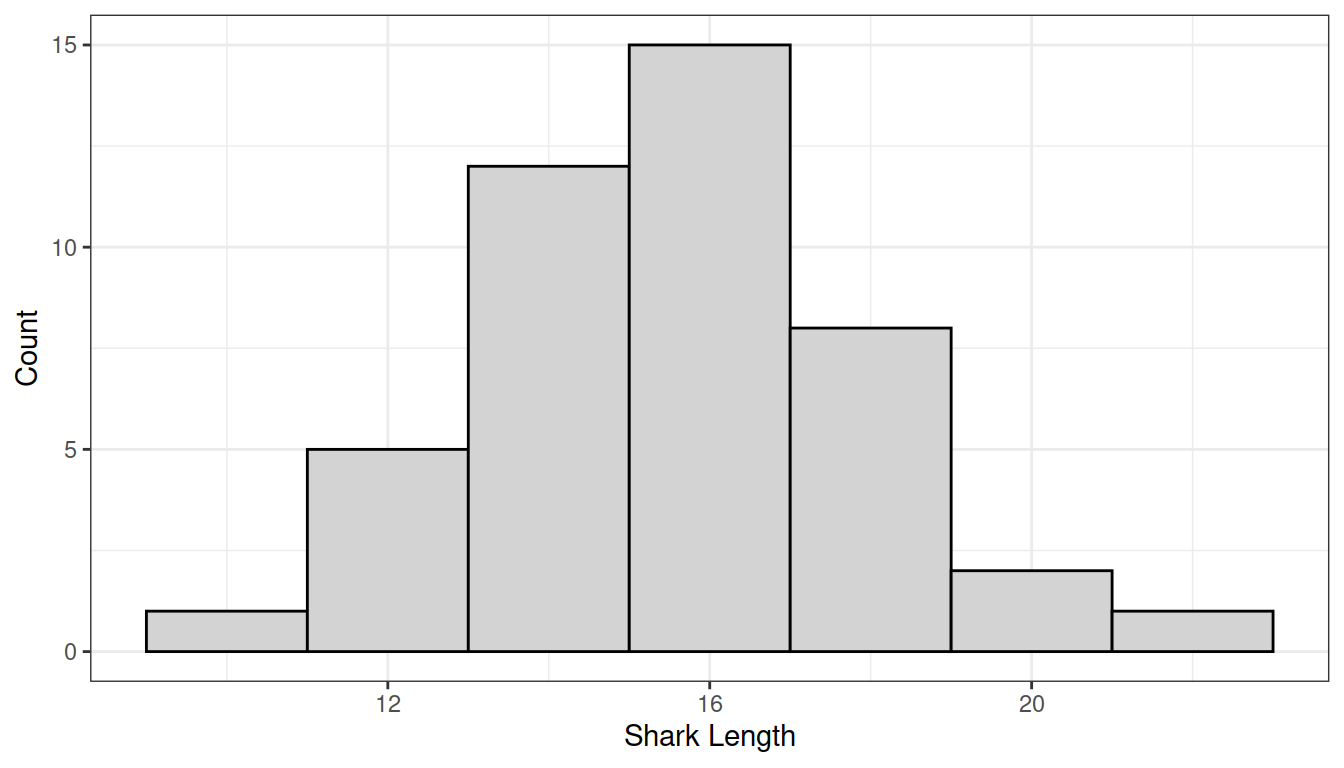
\includegraphics{L03-Scatterplots_Correlation_files/figure-pdf/unnamed-chunk-13-1.pdf}

It's important to note that \(r\) can always be calculated for numeric
data. If we had student numbers as well as a categorical variable that
used 0 to represent black, 1 to represent asian, etc., then we could
technically calculate the correlation coefficient. This would be utterly
meaningless!!!!!

\hypertarget{example-penguins}{%
\subsection{Example: Penguins}\label{example-penguins}}

\includegraphics{L03-Scatterplots_Correlation_files/figure-pdf/unnamed-chunk-14-1.pdf}

This is an example of something called \textbf{Simpson's Paradox}: If we
don't account for the sub-groups, we get the opposite affect! As we can
see in the plot, if we have all the groups together than it looks like a
negative correlation, but once we separate groups each individual group
has a positive correlation.

(Note that I hid the code for this plot - the code I used to ensure the
colours matched and I got the right layout is pretty advanced, and I
also used some tricks along the way.)

\hypertarget{correlation-summary}{%
\subsection{Correlation Summary}\label{correlation-summary}}

\begin{itemize}
\tightlist
\item
  \(r\) is a measure of \textbf{linear} association

  \begin{itemize}
  \tightlist
  \item
    I've said it plenty, I'll say it again: \(r\) does not apply to
    non-linear patterns!
  \item
    Always plot your data before calculating \(r\).
  \end{itemize}
\item
  \(r\) is like a measure of how two variables vary together.

  \begin{itemize}
  \tightlist
  \item
    Formula is similar to the variance formula!
  \end{itemize}
\item
  \(r\) is a number between -1 and 1, with 0 meaning no correlation and
  1 or -1 meaning perfect correlation.

  \begin{itemize}
  \tightlist
  \item
    A negative \(r\) means a negative relationship (i.e.~a line that
    goes down).
  \end{itemize}
\item
  Everything on the ``Comments'' slide is fair game for test questions.
\end{itemize}

\hypertarget{participation-questions-1}{%
\section{Participation Questions}\label{participation-questions-1}}

\hypertarget{q01}{%
\subsection{Q01}\label{q01}}

The correlation coefficient measures the strength of the correlation.

\begin{enumerate}
\def\labelenumi{\arabic{enumi}.}
\tightlist
\item
  True
\item
  False
\end{enumerate}

\hypertarget{q02}{%
\subsection{Q02}\label{q02}}

If \(r < 0\), there is a negative linear correlation.

\begin{enumerate}
\def\labelenumi{\arabic{enumi}.}
\tightlist
\item
  True
\item
  False
\end{enumerate}

\hypertarget{q03}{%
\subsection{Q03}\label{q03}}

Which of the following represents the \emph{strongest} correlation?

\begin{enumerate}
\def\labelenumi{\arabic{enumi}.}
\tightlist
\item
  0.4
\item
  0.7
\item
  -0.8
\item
  0
\end{enumerate}

\hypertarget{q04}{%
\subsection{Q04}\label{q04}}

\vspace{1cm}

What is the best description of the plot on the right?

\begin{enumerate}
\def\labelenumi{\arabic{enumi}.}
\tightlist
\item
  No correlation, has an outlier.
\item
  Strong correlation, has an outlier
\item
  Slight negative correlation
\item
  Shapeless
\end{enumerate}

\begin{Shaded}
\begin{Highlighting}[]
\NormalTok{x }\OtherTok{\textless{}{-}} \FunctionTok{c}\NormalTok{(}\FunctionTok{runif}\NormalTok{(}\DecValTok{99}\NormalTok{, }\DecValTok{0}\NormalTok{, }\DecValTok{10}\NormalTok{), }\DecValTok{11}\NormalTok{)}
\NormalTok{y }\OtherTok{\textless{}{-}} \FunctionTok{c}\NormalTok{(}\FunctionTok{rnorm}\NormalTok{(}\DecValTok{99}\NormalTok{), }\DecValTok{20}\NormalTok{)}

\FunctionTok{ggplot}\NormalTok{() }\SpecialCharTok{+} \FunctionTok{aes}\NormalTok{(}\AttributeTok{x =}\NormalTok{ x, }\AttributeTok{y =}\NormalTok{ y) }\SpecialCharTok{+} \FunctionTok{geom\_point}\NormalTok{() }\CommentTok{\#+ }
\end{Highlighting}
\end{Shaded}

\begin{figure}[H]

{\centering \includegraphics{L03-Scatterplots_Correlation_files/figure-pdf/unnamed-chunk-15-1.pdf}

}

\end{figure}

\begin{Shaded}
\begin{Highlighting}[]
    \CommentTok{\#geom\_smooth(method = "lm", formula = y\textasciitilde{}x, se = FALSE)}
\end{Highlighting}
\end{Shaded}

\hypertarget{extra-context-fitting-a-line}{%
\subsection{Extra context: Fitting a
Line}\label{extra-context-fitting-a-line}}

\vspace{1cm}

A line would try and fit the outlier, which misleads us into thinking
there might be a correlation!

\begin{Shaded}
\begin{Highlighting}[]
\FunctionTok{ggplot}\NormalTok{() }\SpecialCharTok{+} \FunctionTok{aes}\NormalTok{(}\AttributeTok{x =}\NormalTok{ x, }\AttributeTok{y =}\NormalTok{ y) }\SpecialCharTok{+} \FunctionTok{geom\_point}\NormalTok{() }\SpecialCharTok{+} 
    \FunctionTok{geom\_smooth}\NormalTok{(}\AttributeTok{method =} \StringTok{"lm"}\NormalTok{, }\AttributeTok{formula =}\NormalTok{ y}\SpecialCharTok{\textasciitilde{}}\NormalTok{x, }\AttributeTok{se =} \ConstantTok{FALSE}\NormalTok{)}
\end{Highlighting}
\end{Shaded}

\begin{figure}[H]

{\centering \includegraphics{L03-Scatterplots_Correlation_files/figure-pdf/unnamed-chunk-16-1.pdf}

}

\end{figure}

\hypertarget{q05}{%
\subsection{Q05}\label{q05}}

Which statement is \emph{true}.

\begin{enumerate}
\def\labelenumi{\arabic{enumi}.}
\tightlist
\item
  The explanatory variable causes the response.
\item
  The response must be something measured \emph{after} the explanatory
  variable.
\item
  We use the explanatory variable to explain the response, without
  assuming causality.
\item
  The correlation between the explanatory and response variable will be
  positive if the explanatory causes the response, negative if the
  response causes the explanatory.
\end{enumerate}

\hypertarget{q06}{%
\subsection{Q06}\label{q06}}

We can add colour to a plot using what type of variable?

\begin{enumerate}
\def\labelenumi{\arabic{enumi}.}
\tightlist
\item
  Categorical
\item
  Quantitative
\end{enumerate}

\textbf{Exercises:}

\begin{enumerate}
\def\labelenumi{\arabic{enumi}.}
\tightlist
\item
  The following code will draw a plot and calculate the correlation
  coefficient. Currently, it's doing this for the column \texttt{mpg}
  (response) versus the column \texttt{wt} (``weight'', explanatory) in
  the \texttt{mtcars} data which is built in to R.

  \begin{enumerate}
  \def\labelenumii{\alph{enumii}.}
  \tightlist
  \item
    Re-run the code, but replace \texttt{wt} with \texttt{disp} (engine
    displacement), \texttt{hp} (horsepower), \texttt{drat} (rear axle
    ratio, although I couldn't explain this further), and \texttt{qsec}
    (quarter mile time, in seconds). Comment on the apparent pattern and
    the magnitude of the correlation.
  \item
    Change \texttt{wt} to\texttt{cyl}, the number of cylinders. What do
    you notice about the plot, and how does this affect your
    interpretation of the correlation between \texttt{mpg} and
    \texttt{cyl}? Explain why \texttt{cyl} might be better incorporated
    as a categorical variable, even though it is indeed numeric.
  \item
    Repeat part (b) for \texttt{am}, which is ``0'' for automatic
    transmission and ``1'' for manual transmission.
  \end{enumerate}
\end{enumerate}

\begin{Shaded}
\begin{Highlighting}[]
\FunctionTok{plot}\NormalTok{(mpg }\SpecialCharTok{\textasciitilde{}}\NormalTok{ wt, }\AttributeTok{data =}\NormalTok{ mtcars)}
\end{Highlighting}
\end{Shaded}

\begin{figure}[H]

{\centering \includegraphics{L03-Scatterplots_Correlation_files/figure-pdf/unnamed-chunk-17-1.pdf}

}

\end{figure}

\begin{Shaded}
\begin{Highlighting}[]
\FunctionTok{cor}\NormalTok{(mtcars}\SpecialCharTok{$}\NormalTok{mpg, mtcars}\SpecialCharTok{$}\NormalTok{wt)}
\end{Highlighting}
\end{Shaded}

\begin{verbatim}
[1] -0.8676594
\end{verbatim}

\begin{enumerate}
\def\labelenumi{\arabic{enumi}.}
\setcounter{enumi}{1}
\tightlist
\item
  The following figure comes from the article ``Shared neural
  representations and temporal segmentation of political content predict
  ideological similarity'' by De Brujin et al., published in 2023
  (\href{https://www.science.org/doi/10.1126/sciadv.abq5920}{link to
  aricle here}). The star on the plot indicates that they have found a
  statistically significant relationship (more on this next week). Is
  this a strong correlation?
\end{enumerate}

\begin{enumerate}
\def\labelenumi{\arabic{enumi}.}
\setcounter{enumi}{2}
\tightlist
\item
  The following figure comes from the article ``Effect on Blood Pressure
  of Daily Lemon Ingestion and Walking'' by Kato et al., published in
  2013 (\href{https://www.hindawi.com/journals/jnme/2014/912684/}{link
  to article here}). Comment on the shape of this relationship. Recall
  how we described a ``strong'' shape as a shape that remains even if
  some of the data points were removed.
\end{enumerate}

\textbf{Exercises from OpenIntro Biotatistics textbook}

Questions 1.35, 1.36, 1.37.

For further R practice and case studies, see the
\href{https://www.openintro.org/book/statlabs/?labblock=biostat_intro_to_data}{labs
page for the OpenIntro textbook}.

\hypertarget{regression}{%
\chapter{Regression}\label{regression}}

\hypertarget{introduction-2}{%
\section{Introduction}\label{introduction-2}}

These notes are based on Chapter 4 of Baldi \& Moore and Chapter 6.1 to
6.3 in OpenIntro Biostats.

In linear modelling, we have a collection of pairs \(x_i\) and \(y_i\).
We think that there's some sort of relationship between \(x\) and \(y\),
and we think that a line is an adequate way to characterize that
relationship\footnote{Very few things are actually linear, but lines are
  fantastic approximations to many things.}.

Just like we assume that there's a ``true'' population mean, there is
also a ``true'' slope and intercept for the line that characterizes the
relationship between \(x\) and \(y\). In the plot below, the green line
represents the ``true'' relationship between \(x\) and \(y\), and the
data are random values above and below that line\footnote{We assume that
  \(x\) is fixed, but \(y\) has random noise. In other words, \(x\) is
  not a random variable but \(y\) is.}.

\includegraphics{L04-Regression_files/figure-pdf/unnamed-chunk-2-1.pdf}

In high school, you may have learned a line as \(y = mx + b\). In
statistics, we often use latin letters for estimates and greek letters
for population parameters\footnote{Because we think it makes us fancy.
  Note that the Baldi \& Moore textbook uses \(a\), \(b\), and \(e\) for
  everything.}. The population line is thus:

\[
y_i = \alpha + \beta x_i + \epsilon_i
\]

\begin{itemize}
\tightlist
\item
  \(\alpha\) is the \textbf{intercept}.
\item
  \(\beta\) is the \textbf{slope}.

  \begin{itemize}
  \tightlist
  \item
    A 1 unit increase in \(x\) corresponds to a \(\beta\) increase in
    \(y\).
  \end{itemize}
\item
  \(\epsilon_i\) is random noise (\(N(0,\sigma)\)).

  \begin{itemize}
  \tightlist
  \item
    Again, we think of \(x\) as being fixed. The random noise is above
    and below the line, not side to side.
  \end{itemize}
\item
  The formula implies that \(y_i \sim N(\alpha + \beta x_i, \sigma)\),
  since \(y_i\) is centered at \(\alpha + \beta x_i\) but randomly
  varies above and below the line with variance \(\sigma^2\).
\end{itemize}

The word ``regression'' means to go backward. I like to think that we
are ``going backward'' to the population numbers from the sample
values\footnote{Actually, the word comes from ``regressing to the
  mean'', which comes from how children are closer to average height
  than their parents - they go back toward the mean. This is not
  important.}. Any situation where you are estimating a population
parameter is technically a \textbf{regression}, but this terminology is
not useful for this class.

To regress, we \textbf{estimate} the parameters using sample statistics.
For linear regression, we use regular old latin letters instead of the
fancy greek ones. \(a\) is the estimate for \(\alpha\), \(b\) for
\(\beta\), and \(e\) for \(\epsilon\). In order to do find these sample
statistics, we minimize the squared error between the line and the data:

\[e_i^2 = (y_i - a - b x_i)^2\]

In other words, we find \(a\) (for \(\alpha\)) and \(b\) (for \(\beta\))
that make the sum of the squared errors \(e_i\) as small as possible. We
use the squared errors for the same reason we use squared deviations in
the forumla for the variance: so that positive and negative values do
not cancel out\footnote{Also, because the calculus works out so much
  better.}.

The estimates \(a\) and \(b\) are as follows:

\begin{align*}
b &= rs_y/s_x\\
a &= \bar y - b\bar x
\end{align*}

These are called the \textbf{least squares} estimates\footnote{There are
  other ways to estimate these parameters, but they're outside the scope
  of this course. All regression lines that you see in the textbook and
  the notes will be least squares regression lines.}. The equation for
\(b\) is especially important!

In R, these can be calculated as follows. The \texttt{mtcars} data set
is a collection of measurements made on various cars. In this example,
we'll regress the fuel efficiency (in miles per gallon, or mpg) against
the weight of the car.

\begin{Shaded}
\begin{Highlighting}[]
\DocumentationTok{\#\# Load a built{-}in data set}
\FunctionTok{data}\NormalTok{(mtcars) }

\DocumentationTok{\#\# Define which variables are x and y.}
\DocumentationTok{\#\# This isn\textquotesingle{}t necessary, but helps with teaching}
\NormalTok{x }\OtherTok{\textless{}{-}}\NormalTok{ mtcars}\SpecialCharTok{$}\NormalTok{wt}
\NormalTok{y }\OtherTok{\textless{}{-}}\NormalTok{ mtcars}\SpecialCharTok{$}\NormalTok{mpg}

\DocumentationTok{\#\# Calculate the estimates by hand}
\NormalTok{b }\OtherTok{\textless{}{-}} \FunctionTok{cor}\NormalTok{(x, y) }\SpecialCharTok{*} \FunctionTok{sd}\NormalTok{(y) }\SpecialCharTok{/} \FunctionTok{sd}\NormalTok{(x)}
\NormalTok{a }\OtherTok{\textless{}{-}} \FunctionTok{mean}\NormalTok{(y) }\SpecialCharTok{{-}}\NormalTok{ b }\SpecialCharTok{*} \FunctionTok{mean}\NormalTok{(x)}

\DocumentationTok{\#\# Print the estimates }
\FunctionTok{c}\NormalTok{(a, b)}
\end{Highlighting}
\end{Shaded}

\begin{verbatim}
[1] 37.285126 -5.344472
\end{verbatim}

\begin{Shaded}
\begin{Highlighting}[]
\DocumentationTok{\#\# Use the built{-}in functions}
\FunctionTok{summary}\NormalTok{(}\FunctionTok{lm}\NormalTok{(y }\SpecialCharTok{\textasciitilde{}}\NormalTok{ x))}
\end{Highlighting}
\end{Shaded}

\begin{verbatim}

Call:
lm(formula = y ~ x)

Residuals:
    Min      1Q  Median      3Q     Max 
-4.5432 -2.3647 -0.1252  1.4096  6.8727 

Coefficients:
            Estimate Std. Error t value Pr(>|t|)    
(Intercept)  37.2851     1.8776  19.858  < 2e-16 ***
x            -5.3445     0.5591  -9.559 1.29e-10 ***
---
Signif. codes:  0 '***' 0.001 '**' 0.01 '*' 0.05 '.' 0.1 ' ' 1

Residual standard error: 3.046 on 30 degrees of freedom
Multiple R-squared:  0.7528,    Adjusted R-squared:  0.7446 
F-statistic: 91.38 on 1 and 30 DF,  p-value: 1.294e-10
\end{verbatim}

From this line, we can make \textbf{predictions} about new points by
simply plugging in the \(x\) value. For example, let's say we wanted to
guess the mpg of a car that weighs 3,000 lbs. In the data, the units for
weight are 1000 lbs, so this means plugging a value of \texttt{wt=3}
into the data.

\begin{Shaded}
\begin{Highlighting}[]
\NormalTok{a }\SpecialCharTok{+}\NormalTok{ b}\SpecialCharTok{*}\DecValTok{3}
\end{Highlighting}
\end{Shaded}

\begin{verbatim}
[1] 21.25171
\end{verbatim}

So we would guess that a 3 ton car would have a fuel efficiency of 21.25
miles per gallon. Let's look at this on a plot:

\begin{Shaded}
\begin{Highlighting}[]
\FunctionTok{plot}\NormalTok{(y }\SpecialCharTok{\textasciitilde{}}\NormalTok{ x)}
\FunctionTok{points}\NormalTok{(}\DecValTok{3}\NormalTok{, a }\SpecialCharTok{+}\NormalTok{ b}\SpecialCharTok{*}\DecValTok{3}\NormalTok{, }\AttributeTok{col =} \StringTok{"red"}\NormalTok{, }\AttributeTok{pch =} \DecValTok{16}\NormalTok{)}
\end{Highlighting}
\end{Shaded}

\begin{figure}[H]

{\centering \includegraphics{L04-Regression_files/figure-pdf/unnamed-chunk-5-1.pdf}

}

\end{figure}

It looks like this is somewhere around where we would expect.

If we repeat this for every possible \(x\) value, we get the regression
line below:

\begin{Shaded}
\begin{Highlighting}[]
\FunctionTok{plot}\NormalTok{(y }\SpecialCharTok{\textasciitilde{}}\NormalTok{ x)}
\FunctionTok{points}\NormalTok{(}\DecValTok{3}\NormalTok{, a }\SpecialCharTok{+}\NormalTok{ b}\SpecialCharTok{*}\DecValTok{3}\NormalTok{, }\AttributeTok{col =} \StringTok{"red"}\NormalTok{, }\AttributeTok{pch =} \DecValTok{16}\NormalTok{)}
\DocumentationTok{\#\# abline adds a line with slope b and intercept a to a plot.}
\FunctionTok{abline}\NormalTok{(}\AttributeTok{a =}\NormalTok{ a, }\AttributeTok{b =}\NormalTok{ b, }\AttributeTok{col =} \StringTok{"red"}\NormalTok{)}
\end{Highlighting}
\end{Shaded}

\begin{figure}[H]

{\centering \includegraphics{L04-Regression_files/figure-pdf/unnamed-chunk-6-1.pdf}

}

\end{figure}

We cal also see the values of \(e\), the residuals.

\begin{Shaded}
\begin{Highlighting}[]
\NormalTok{e }\OtherTok{\textless{}{-}}\NormalTok{ y }\SpecialCharTok{{-}}\NormalTok{ (a }\SpecialCharTok{+}\NormalTok{ b}\SpecialCharTok{*}\NormalTok{x)}
\FunctionTok{plot}\NormalTok{(e }\SpecialCharTok{\textasciitilde{}}\NormalTok{ x, }\AttributeTok{main =} \StringTok{"Plot of the Residuals"}\NormalTok{)}
\DocumentationTok{\#\# abline can also draw a line with slope 0 (horizontal)}
\FunctionTok{abline}\NormalTok{(}\AttributeTok{h =} \DecValTok{0}\NormalTok{, }\AttributeTok{col =} \StringTok{"grey"}\NormalTok{)}
\end{Highlighting}
\end{Shaded}

\begin{figure}[H]

{\centering \includegraphics{L04-Regression_files/figure-pdf/unnamed-chunk-7-1.pdf}

}

\end{figure}

\hypertarget{regression-facts}{%
\section{Regression Facts}\label{regression-facts}}

Here are some facts about the least squares regression line:

\begin{itemize}
\tightlist
\item
  The point \((\bar x, \bar y)\) is always on the line.

  \begin{itemize}
  \tightlist
  \item
    Least squares regression can be seen as putting a line through
    \((\bar x, \bar y)\) and rotating it until the squared error is the
    smallest.
  \end{itemize}
\item
  \(s_y\ge 0\) and \(s_x\ge 0\), so whenever \(r > 0\), we know that
  \(b > 0\).

  \begin{itemize}
  \tightlist
  \item
    The slope has the same sign as the correlation. Otherwise, the slope
    could be pretty much any number, regardless of the correlation.
  \item
    If \(r = 0\), then \(b = 0\), and vice versa.
  \item
    Other than the sign and the special case of \(r=0\), there is no way
    to tell the value of \(r\) if all you know is \(b\).
  \end{itemize}
\item
  For \(r\), the distinction between \(y\) and \(x\) doesn't matter.

  \begin{itemize}
  \tightlist
  \item
    For the regression line, it \emph{absolutely} matters!
  \end{itemize}
\item
  The sum of the errors is 0.
\end{itemize}

\begin{Shaded}
\begin{Highlighting}[]
\DocumentationTok{\#\# The prediction at mean(x) is equal to mean(y)}
\DocumentationTok{\#\# In other words, (mean(x), mean(y)) is a point on the line}
\NormalTok{a }\SpecialCharTok{+}\NormalTok{ b }\SpecialCharTok{*} \FunctionTok{mean}\NormalTok{(x)}
\end{Highlighting}
\end{Shaded}

\begin{verbatim}
[1] 20.09062
\end{verbatim}

\begin{Shaded}
\begin{Highlighting}[]
\FunctionTok{mean}\NormalTok{(y)}
\end{Highlighting}
\end{Shaded}

\begin{verbatim}
[1] 20.09062
\end{verbatim}

\begin{Shaded}
\begin{Highlighting}[]
\DocumentationTok{\#\# Correlation doesn\textquotesingle{}t care about order}
\FunctionTok{cor}\NormalTok{(x, y)}
\end{Highlighting}
\end{Shaded}

\begin{verbatim}
[1] -0.8676594
\end{verbatim}

\begin{Shaded}
\begin{Highlighting}[]
\FunctionTok{cor}\NormalTok{(y, x)}
\end{Highlighting}
\end{Shaded}

\begin{verbatim}
[1] -0.8676594
\end{verbatim}

\begin{Shaded}
\begin{Highlighting}[]
\DocumentationTok{\#\# Theoretically 0, but computers aren\textquotesingle{}t perfectly precise}
\DocumentationTok{\#\# Note: e{-}14 refers to 10\^{}{-}14, or 14 zeroes before the first digit}
    \CommentTok{\# So, pretty close to 0.}
\FunctionTok{sum}\NormalTok{(e) }
\end{Highlighting}
\end{Shaded}

\begin{verbatim}
[1] 1.065814e-14
\end{verbatim}

\hypertarget{percent-of-variation-explained}{%
\section{Percent of Variation
Explained}\label{percent-of-variation-explained}}

Because of some mathematical quirks, \(r^2\), the squared value of
\(r\), can be interpreted as:

\begin{quote}
\textbf{The percent of variation in \(y\) that can be ``explained'' by
the linear model}.\footnote{Usually \(r^2\) is labelled \(R^2\) for
  historical reasons. Capitalization matters in math; it's just
  coincidence that both lower case and upper case mean the same thing
  here.}
\end{quote}

The value of \(r^2\) can be calculated as: \[
R^2 = r^2 = \frac{\text{Variance of the predicted }y\text{-values}}{\text{Variance of the observed }y\text{-values}}
\]

I'll explain this in steps. The first plot below shows just the values
in \(y\). This collection of values has a own mean and variance.

The second plot shows the change in variance that the line ``explains''.
Instead of deviations above and below the mean, the variance can now be
characterized as the deviations above and below the regression line.
This variance will always be lower than the variance of \(y\) without
incorporating \(x\)\footnote{Except when \(r=0\), can you explain why?}.

The third plot shows where this variance went. \emph{The line itself has
variance}; there is deviation in the line above and below the mean of
\(y\). This is the variance that gets explained by incorporating \(x\)!
If you consider one of the points in \(y\), say \(y_1\), the distance
between \(y_1\) and \(\bar y\) can be split up into the difference
between \(\bar y\) and the regression line plus the distance between the
regression line and \(y_1\).

\includegraphics{L04-Regression_files/figure-pdf/unnamed-chunk-9-1.pdf}

The rest of the variance is left \textbf{unexplianed}. No regression
will ever be perfect unless we are studing a very very simple .

To see this a different way, consider what happens when
\(r = 0\)\footnote{Therefore the slope will also be 0.}. This will just
be a horizontal line, and none of the variance is explained. On the
other had, if \(r = 1\) then all of the points will be exactly on the
line. All of the variance in \(y\) has been explained by the regression
against \(x\) - there's no variance left to be explained!\footnote{Statistics
  is \emph{still} just the study of variance.}

Notice how the R output includes

\hypertarget{extensions-and-cautions}{%
\section{Extensions and Cautions}\label{extensions-and-cautions}}

\hypertarget{prediction}{%
\subsection{Prediction}\label{prediction}}

For a new \(x\) value, \[y = a + bx\] is the \textbf{predicted} value of
\(y\). That is, if we have an \(x\) value, we can plug it into the
equation and find out what value of \(y\) we would expect.

Note: There is still variance around this prediction! Our ``expected''
value will never be exactly equal to the truth - The value of \(y\) at a
given value of \(x\) follows a normal distribution\footnote{Our
  \textbf{prediction} is just us guessing the mean value of \(y\) at
  different values of \(x\).}, and the probability of a single point is
0!

\hypertarget{extrapolation}{%
\subsection{Extrapolation}\label{extrapolation}}

\textbf{Extrapolation} is what happens when prediction goes wrong. In
particular, it's what happens when we try to make a prediction at an
\(x\) value where we don't have any data. Usually this means we're
predicting an \(x\) value far above or far below the range of our data,
but it can also happen if there's a gap in the middle of our data.

In the plot below, the black dots are the original data, and we're
trying to predict a new value at \(x = 25\). The red line is the true
model that I generated the data from. The black line represents a linear
model. This model fits the original data quite well\footnote{Even though
  it's not the true relationship, it's a reasonable approximation.}, but
predictions are completely inappropriate for values outside the data.

\includegraphics{L04-Regression_files/figure-pdf/unnamed-chunk-10-1.pdf}

\hypertarget{lurking-variables}{%
\subsection{Lurking Variables}\label{lurking-variables}}

The black line in the plot below represents a regression where all of
the data was lumped together. As we can see, this line does not seem to
fit the data well. There is a hidden relationship in the the data - the
green points and the red points should be considered
separately\footnote{Possibly as a blocking variable.}.

\includegraphics{L04-Regression_files/figure-pdf/unnamed-chunk-11-1.pdf}

A more serious consequence of a lurking variable has shown up before in
the Palmer penguins data. In that example, the lurking variable actually
\textbf{reversed} the correlation - if we lumped the groups together we
got a negative correlation (and therefore negative slope), but if we
looked at the groups individually we got positive associations in all of
the groups! This is called \textbf{Simpson's Paradox}, and basically
means that we have to be very careful about interpreting correlations!

\includegraphics{L04-Regression_files/figure-pdf/unnamed-chunk-12-1.pdf}

\hypertarget{probability-background}{%
\chapter{Probability Background}\label{probability-background}}

Please pay attention to the margin notes.\footnote{These things!} They
often contain important information.\footnote{Or silliness.}

These notes are based on Chapter 9 in Baldi \& Moore (4th edition).
Chapter 2 of \href{https://www.openintro.org/book/biostat}{OpenIntro
Biostatics} is also a great (free) resource.

\hypertarget{defining-probability-with-dice}{%
\section{Defining Probability with
Dice}\label{defining-probability-with-dice}}

I find that the easiest way is to build this up by examples. Let's start
with rolling a dice.\footnote{The singular form ``die'' is dieing out;
  the dictionary lists ``dice'' as singular noun, and the singular
  ``dice'' is clearer for new English speakers.} Let's say you rolled
the dice, and you got a 3. This is called a \textbf{simple event}. The
collection of all \textbf{simple events} is called the \textbf{Sample
Space}, which in this case is \(\mathcal S\)=\{1,2,3,4,5,6\}.

Now, suppose that you're about to roll a dice. You might be curious
about whether it's a 1, 2, 3, 4, 5, or a 6, but you might only care
about the \textbf{event} that the outcome is even. Since there are
multiple simple events that make up this event, it is called a
\textbf{compound event}.

There's no way for you to know what's going to happen, but you know all
of the possibilities and you know how likely they all are.\footnote{Assuming
  there's nothing unusual about your dice.} This is called a
\textbf{Probability Model}: The sample space along with the probability
of all of the events.

I said ``the probability of all events'', but this is more complicated
than it may seem and requires some explanation. For something like
rolling a dice, you only need to know the probability of each simple
event. Compound events, like the probability that the outcome is even,
can be determined from these simple events.

Suppose you're playing a game where, if the outcome of the dice is less
than a certain cutoff value you get to roll again (e.g., your character
has a special ability that allows re-rolling of dice, but the re-roll
condition depends on the situation). You know the probability of all of
the simple events, but you need to know the cutoff value to actually
compute any probabilities. Without the cutoff value, you cannot define
the probability model.

For a dice, the probability model is simply: Each number has a
probability of 1 in 6. But what does this mean? There are two
perspectives on what a ``probability'' is: The Frequentist approach and
the Bayesian approach. In this class we're only going to learn the
Frequentist definition of probability, but if you're interested in
learning more I'm happy to talk.\footnote{Most of my work uses the
  Bayesian definition.}

\textbf{Probability} (Frequentist Definition): The long run frequency of
observing an event. In other words, it's the number of times an event is
observed divided by the number of trials after doing a near-infinite
number of trials.

For the dice, if we rolled the dice 60 times, we would expect 10 of
those rolls to be a 1, 10 of them to be a 2, etc. Due to randomness, we
won't get exactly that, but this is what we would expect. If we rolled
600 dice, we would expect 100 to be 1, etc. As we roll more dice, we get
closer to the proportion of 1/6. The plot below this demonstrates this -
it is the number of times that a dice was 1 divided by the number of
trials, with the number of trials being increased. Notice how it takes a
while for the ``empirical'' probability to reach the theoretical
probably; as the number of trials approaches infinity, the proportion of
rolls that showed a 1 will approach 1/6.

\includegraphics{L05-Probability_files/figure-pdf/unnamed-chunk-1-1.pdf}

\hypertarget{calculating-probability-with-dice}{%
\section{Calculating Probability with
Dice}\label{calculating-probability-with-dice}}

First, let's introduce some notation. I will use P(x) to mean ``The
probability of x''. In some cases, the context will be clear, such as:

\begin{itemize}
\tightlist
\item
  ``The probability of rolling a 1'' = P(1)
\item
  ``The probability of rolling an even number'' = P(even)
\item
  ``The probability of \emph{not} rolling a 1'' = 1 - P(1)\footnote{This
    is called a \textbf{complement}.}
\end{itemize}

For this section, we'll assume that
P(1)=P(2)=P(3)=P(4)=P(5)=P(6)=1/6.\footnote{The sum of all probabilities
  must be 1.}

\hypertarget{or}{%
\subsection{``Or''}\label{or}}

What's the probability that we roll an even number? The even numbers are
2, 4, and 6, so what we're really asking is ``What's the probability
that we roll a 2, 4, \textbf{or} a 6?'' In this case, the probability is
P(2 or 4 or 6) = P(2)+P(4)+P(6) = 1/6 + 1/6 + 1/6 = 3/6 = 0.5.

We also could have figured out this probability by noting that half of
the values are even, so a probability of 0.5 makes sense. It's a good
thing when our intuition matches our answer, as we'll see next.

Let's consider the probability that the dice is even\^{} (which we will
denote P(even)) \textbf{or} it's strictly larger than 3 (denoted
P(\textgreater3)). This means the dice is either 2, 4, or 6, or it's 4,
5, 6. Since there are 4 different numbers (2, 4, 5, and 6) that would
match the criteria, the probability is 4/6. Let's use our ``or'' rules
to verify this!

The probability that the dice is even is 1/2. The probabilty that the
dice is larger than 3 is also 1/2. So, obviously, P(even or
\textgreater3) = P(even) + P(\textgreater3) = 1/2 + 1/2 = 1.

Wait.

That can't be right.

I think you may be able to see what went wrong. The P(even) = P(2) +
P(4) + P(6), and P(\textgreater3) = P(4) + P(5) + P(6). When we did
P(even) + P(\textgreater3), we added P(4) and P(6) twice! To get the
right answer, we need to fix this. Since we added them twice, we must
subtract them once. This brings us to\ldots{}

\hypertarget{the-addition-rule-for-or}{%
\subsection{The Addition Rule for
``or''}\label{the-addition-rule-for-or}}

For any two events A and B,\footnote{For example, A = ``Even'', B =
  ``\textgreater3''.} the \textbf{Addition Rule} states:

\begin{align}P(A\; or\; B) = P(A) + P(B) - P(A\; and\; B).\end{align}

First, note that the probability of both events is P(Even \textbf{and}
\textgreater3) = P(4) + P(6), since 4 and 6 are both even and larger
than 3.

\begin{align*}
 P(Even\; or\; >3) & = P(Even) + P(>3) - P(Even\; and\; >3)\\
& = [P(2) + P(4) + P(6)] + [P(4) + P(5) + P(6)] - [P(4) + P(6)]\\
& =  P(2) + P(4) + P(5) + P(6)\\
& = 1/6 + 1/6 + 1/6 + 1/6\\
& = 4/6
\end{align*} \normalsize

\hypertarget{and-part-1}{%
\subsection{``and'': Part 1}\label{and-part-1}}

The word ``and'' came up in the addition rule, and so I should give a
good definition of ``and''. When we talk about events A and B, P(A and
B) refers to the probability that they both happen together. It's most
helpful to see this as a Venn diagram:

P(A) is the area of the circle labelled A, P(B) is the area of the
circle labelled B, and P(A and B) is the area of the overlap between
these two circles. P(A or B) is the total shaded area, including the
yellow-green, green, and dark green.

You can see the Addition Rule at work here. If you add the area of A
(which includes P(A and B)) to the area of B (which also includes P(A
and B)), you've added P(A and B) twice!

There are two formulas for P(A and B). The first one is found by
rearranging the formula for P(A or B):

\begin{align*}
\small P(A\; or\; B) &\small = P(A) + P(B) - P(A \;and\; B)\\
\small P(A\; and\; B) &\small = P(A) + P(B) - P(A \;or\; B)
\end{align*}

When in doubt, just remember P(A\_B) = P(A) + P(B) - P(A\_B), then put
``or'' in one blank and ``and'' in the other.

This formula won't always get you to the solution, though. There will be
many times where neither ``and'' nor ``or'' will be obvious, and we'll
need to do some more work to get them. We have special formulas for
``and'', so we'll usually try to figure out the ``and'' and then use it
to figure out the ``or''\footnote{This lecture has some of the weirdest
  sentences.}.

\hypertarget{given-conditional-probabilities}{%
\subsection{``given'': Conditional
Probabilities}\label{given-conditional-probabilities}}

A \emph{condition} is something that must happen before you can proceed.
A \textbf{conditional probability} is a probability that requires
something else to happen, and usually involves a more complicated setup.

Let's look at another scenario. Let's say I told you that the number on
the dice was larger than 3. What's the probability that the number on
the dice is a 4? Intuiutively, it's 1/3, since there are 3 possible
numbers. Our notation fails us here, P(4) denotes the probability that
the dice is a 4, which we already determined was 1/6. We can't use P(4)
for two things, so we need to add some notation.

In this case, the solution is to use a vertical bar, ``\textbar{}'',
which is pronounced ``given''. We write ``P(dice is 4 \textbar{} dice is
greater than 3) = 1/3'',\footnote{P(4 \textbar{} \textgreater3) just
  looks too confusing, so I added some words.} which is read as ``The
probability that the dice is 4, \textbf{given that} the dice is larger
than 3.''

A very important thing happened here: when we used a conditional
probability (``given that''), we \textbf{restricted the sample space}.
When we ``condition'' on an event, it means that we're only looking at
cases where that event happened. ``The probability that the dice is 4,
given that the dice is larger than 3'' is another way of saying that
we're only considering events where the dice roll is greater than 3; we
don't care about 1, 2, or 3.

We defined ``probability'' as the total number of events divided by the
total number of trials. For conditional probabilities, this means that
we're only looking at \emph{some of} the trials.

\begin{align*}
\small P(dice\; is\; 4\; |\; dice\; is >3) = \frac{\#\; ways\;dice\;can\;be\;4\;}{\#\;ways\;dice\;can\;be\;>3}=\frac{1}{3}
\end{align*}

\textbf{This formula is incorrect}: ``The number of ways that a dice can
be 4'' depends on the condition. For instance, the number of ways that a
dice can be 2 is 0 since we're told it's larger than 3. We are actually
looking at the number of ways that the dice can be both 4 \textbf{and}
greater than 3. Let's incorporate this information:

\begin{align*}
\small P(dice\; is\; 4\; |\; dice\; is >3) = \frac{\#\; ways\;dice\;can\;be\;4\;\;and\;>3}{\#\;ways\;dice\;can\;be\;>3}=\frac{1}{3}
\end{align*}

For any two events A and B, \textbf{conditional probabilities} are
defined as follows:\footnote{To remember this, I like to imagine the
  vertical bar falling on the the B and pushing it into the denominator.}

\begin{align*}
\small P(A | B) = \frac{P(A\;and\; B)}{P(B)}
\end{align*}

The equation above is a \emph{definition}. It's not the result of
something else, it's the way we define conditional probability.
Rearranging it, though, gives us an important result.

\hypertarget{and-part-2-the-multiplication-rule}{%
\subsection{``and'' Part 2: The Multiplication
Rule}\label{and-part-2-the-multiplication-rule}}

For any two events A and B, the \textbf{Multiplication Rule} states:

\begin{align*}
\small P(A\; and\; B) = P(A|B)P(B)
\end{align*}

Note that P(B\textbar A) = P(A and B)/P(A), so the multiplication rule
can be extended:

\begin{align*}
\small P(A\; and\; B) &\small = P(A|B)P(B)\\
\small P(A\; and\; B) &\small = P(B|A)P(A)
\end{align*}

In other words, you can write it either way as long as the event that
comes after the ``\textbar{}'' also appears on it's own.

Let's use this to answer the following question: What's the probability
that a dice is larger than 3 \textbf{and} even? By intuition, this
should be 2/6 since there are two cases where both are true, but let's
verify with math!

First, recall that P(\textgreater3) and P(even) are both 1/2.

P(\textgreater3 \textbar{} even) means that we're look at the number of
dice rolls that are larger than 3, but we're only considering even dice
rolls. We have 3 total dice rolls that are even, and 2 of those are
larger than 3, so this probability is 2/3. Using the multiplication
rule, P(\textgreater3 and even) = P(\textgreater3 \textbar{}
even)*P(even) = (2/3)*(1/2) = 2/6, which is what we got before!

The other way works out the same. Given that the roll is larger than 3,
there are 2 even rolls, which means that P(even \textbar{}
\textgreater3) = 2/3. P(\textgreater3 and even) = P(even \textbar{}
\textgreater3)*P(even) = (2/3)*(1/2) = 2/6, which is what we got before!

\hypertarget{special-cases-independent-or-disjoint}{%
\subsection{Special Cases: Independent or
Disjoint}\label{special-cases-independent-or-disjoint}}

\hypertarget{disjoint-a.k.a.-mutually-exclusive}{%
\subsection{Disjoint, a.k.a. Mutually
Exclusive}\label{disjoint-a.k.a.-mutually-exclusive}}

\textbf{Disjoint} events, also called \textbf{mutually exclusive}
events, are events that \emph{cannot} occur together. For example, the
event that you roll a 4 and it's also a 3. This simply does not work, so
the probability is 0.

More formally, A and B are \textbf{disjoint} if P(A and B) = 0.

\hypertarget{the-addition-rule-for-disjoint-events}{%
\subsection{The Addition Rule for Disjoint
Events}\label{the-addition-rule-for-disjoint-events}}

If A and B are disjoint, then P(A or B) = P(A) + P(B).\footnote{Not an
  important point: This is a rule, not a result. The General Addition
  Rule is a result of this rule, not the other way around.}

This is actually why we were able to say P(even) = P(2 or 4 or 6) = P(2)
+ P(4) + P(6) = 3/6: the events ``2'', ``4'', and ``6'' are disjoint.

\hypertarget{independent}{%
\subsection{Independent}\label{independent}}

Two events are \textbf{independent} if the knowledge of one event tells
you nothing about the other.\footnote{The opposite of
  \textbf{independence} is \textbf{dependence}.} For instance, if I flip
two different coins and tell you that the first one was Heads, you still
only have a 50/50 chance of guessing the second one.

Notice the phrasing in the previous sentence: ``If I tell you that the
first one is heads\ldots{}'' That is, I'm \emph{restricting the sample
space}. Independence is all about conditional probabilities!

Formally, A and B are independent if P(A \textbar{} B) = P(A).

This adds further insight into conditional probabilities: P(A\textbar B)
is how likely A is, given that you know B happened. Knowledge of B
changes your guess of the likelihood of A. If it doesn't change your
guess, then they are independent.\footnote{Just like in correlations,
  dependence does \emph{not} imply causation!}

The following app demonstrates this concept:

\begin{Shaded}
\begin{Highlighting}[]
\NormalTok{shiny}\SpecialCharTok{::}\FunctionTok{runGitHub}\NormalTok{(}\AttributeTok{repo =} \StringTok{"DBecker7/DB7\_TeachingApps"}\NormalTok{, }
    \AttributeTok{subdir =} \StringTok{"Apps/indep"}\NormalTok{)}
\end{Highlighting}
\end{Shaded}

Another lesson to take from the app above: Independence doesn't look
special. You can't just tell that things are independent by looking at
them.

\hypertarget{the-multiplication-rule-for-independent-events}{%
\subsection{The Multiplication Rule for Independent
Events}\label{the-multiplication-rule-for-independent-events}}

Any time I see a conditional probability, I immediately write down the
formula. For dependence, we are saying:

P(A\textbar B) = P(A and B)/P(B)

which is the same as

P(A and B) = P(A\textbar B)P(B)\footnote{This equation is \emph{always}
  true.}

If two events are \textbf{independent}, then P(A\textbar B)=P(A),
therefore:

P(A and B) \(\stackrel{indep}{=}\) P(A)*P(B)\footnote{The ``\(indep\)''
  over the equals sign is there to specify that this is only true if
  events are independent.}

Get this tattood backwards on your forehead so you see it every time you
look at yourself in the mirror: \textbf{P(A and B) is ONLY equal to
P(A)*P(B) when A and B are independent!!!} Some textbooks start with
this rule then move to the general rule, but far too many students start
using P(A and B) = P(A)P(B) as if it's always true. My entire thesis is
based on whether you can say two things are independent, so it's kind of
a sore spot for me. DO NOT MIX THIS UP.

For example, are the events ``even'' and ``\textgreater3'' independent?
If you know that the dice roll is \textgreater3, then there's a 2/3
chance that it's even. That is, P(even\textbar\textgreater3) = 2/3
\(\ne\) 1/2 = P(even), so it's not independent.

Alternatively, we can calcuate P(even and \textgreater3) = 2/3, but
P(even)*P(\textgreater3) = (1/2)*(1/2) = 1/4. Since 2/3 \(\ne\) 1/4,
these events are not independent.

\hypertarget{disjoint-means-dependent}{%
\subsection{\texorpdfstring{Disjoint means
\emph{Dependent}}{Disjoint means Dependent}}\label{disjoint-means-dependent}}

\textbf{Independence} can be defined as ``if you know that one event
happened, you have no knowledge of the other event.'' \textbf{Disjoint}
can be defined as ``if you know one event happened, you know for sure
that the other one \emph{did not} happen.'' If two events are disjoint,
they must be \textbf{dependent}. In fact, knowledge of one event means
that you for sure know about the other - the exact opposite of
independence!

\ldots{} except when one event is impossible. For instance, P(even and
7) = 0 since there are no dice rolls that are both even and 7, but this
is also equal to P(even)*P(7) = 0 since there are no dice rolls that are
7.

\hypertarget{word-problems}{%
\section{Word Problems}\label{word-problems}}

Question 10.6 from the textbook:\footnote{Baldi, B. and DS. Moore. 2018.
  \emph{The Practice of Statistics in the Life Sciences.} 4th Edition,
  W.H. Freeman and Company.}

The National Survey on Drug Use and Health reports that 18.1\% of all
adults in the United States had a mental illness in 2014. Among adults
with a substance use disorder, 39.1\% had a mental illness. By
comparison, only 16.2\% of adults without a substance use disorder had a
mental illness. The report also states that 3.3\% of American adults had
both a mental illness and a substance use disorder. Use the notation MI
and SUD for mental illness and substance abuse disorder, respectively.

\begin{enumerate}
\def\labelenumi{\alph{enumi}.}
\tightlist
\item
  Express the four percents cited here as probabilities for a randomly
  selected American adult. Use proper probability notation.
\item
  Obtain the probability P(SUD\textbar MI). Write a sentence reporting
  this probability in context.
\end{enumerate}

Solutions:

\begin{enumerate}
\def\labelenumi{\alph{enumi}.}
\tightlist
\item
  There are a couple of probabilities:

  \begin{itemize}
  \tightlist
  \item
    ``18.1\% of all adults in the United States had a mental illness'':
    P(MI) = 18.1
  \item
    ``Among adults with a substance use disorder, 39.1\% had a mental
    illness.'' The part that says ``among adults with SUD'' means that
    we're only looking at people with SUD; we're \emph{restricting the
    sample space}. This is a condition, so our answer must be P(\_
    \textbar{} SUD) = \_\_. The blanks can be filled in as
    P(MI\textbar SUD) = 0.391.
  \item
    ``16.2\% of adults without a substance use disorder had a mental
    illness.'' The part that says ``adults without a SUD'' is also
    \emph{restricting the sample space}, so our probability statement
    will be P(\_\_ \textbar{} no SUD) = \_\_. The blanks are filled in
    as P(MI \textbar{} no SUD) = 0.162.\footnote{This is a great place
      to mention: There's absolutely no reason why P(A\textbar B) +
      P(A\textbar{} not B) should add to 1.}
  \item
    ``3.3\% of American adults had both a MI and a SUD''. This clearly
    states \textbf{and}, so we are looking at P(MI and SUD) = 0.033
  \end{itemize}
\end{enumerate}

Part b. is going to take a few steps. Let's write down all the formulas
that might help. Firstly. there's no ``or'', so that probably won't do
it.

\begin{itemize}
\tightlist
\item
  \emph{Want}: P(SUD\textbar MI)

  \begin{itemize}
  \tightlist
  \item
    P(SUD\textbar MI) = P(SUD and MI)/P(MI), so we need P(SUD and MI)
    and P(MI).
  \end{itemize}
\item
  \emph{Have}:

  \begin{itemize}
  \tightlist
  \item
    P(MI) = 0.181
  \item
    P(MI \textbar{} SUD) = 0.391
  \item
    P(MI \textbar{} no SUD) = 0.162
  \item
    P(MI and SUD) = 0.033
  \end{itemize}
\end{itemize}

Both P(SUD and MI) and P(MI) are given in the question, so our answer is
simply:

\begin{quote}
P(SUD \textbar{} MI) = P(SUD and MI)/P(MI) = 0.033/0.181 = 0.1823
\end{quote}

Therefore 18.23\% of people with mental illness have substance abuse
disorder.

Compare this value to P(MI \textbar{} SUD) = 0.391. In general, there is
no easy relationship between P(A \textbar{} B) and P(B \textbar{} A). If
you know what P(A \textbar{} B) is, you can't really guess at what P(B
\textbar{} A) is; you need a lot more information!

\hypertarget{two-way-tables}{%
\section{Two-Way Tables}\label{two-way-tables}}

I rigorously collected the following data\footnote{Source: I made it up.}
on programming language usage for different disciplines using the most
appropriate sampling methods.

\begin{longtable}[]{@{}lllll@{}}
\toprule\noalign{}
& Stats & Math & Comp Sci & Total \\
\midrule\noalign{}
\endhead
\bottomrule\noalign{}
\endlastfoot
R & 90 & 30 & 40 & 160 \\
Python & 10 & 60 & 100 & 170 \\
MatLab & 15 & 60 & 15 & 90 \\
Julia & 10 & 10 & 1 & 21 \\
\textbf{Total} & 125 & 160 & 156 & 431 \\
\end{longtable}

From this table, we can calculate \textbf{marginal} and
\textbf{conditional} probabilities.

\textbf{Marginal} probabilities are calculated from the margins, which
means that we ignore one of the variables. For example, P(Math) =
160/431 and P(Julia) = 21/431. Both of these proportions are based on
the margins - they don't take the other variable into account.

\textbf{Conditional} probabilities are the same idea as we saw earlier.
Again, we are \emph{restricting our sample space} by conditioning on
another variable. For example, P(R \textbar{} Stats) = 90/125, whereas
P(Stats \textbar{} R) = 90/160. The conditioning event determines which
row/column we use. When we condition on Stats, we \emph{only} look at
the column labelled stats - we do not consider any of the other numbers.
This is why P(R \textbar{} Stats) has a numerator of 125, rather than
431.

You should be familiar with the following calculations:

\begin{enumerate}
\def\labelenumi{\arabic{enumi}.}
\tightlist
\item
  P(Stats) = 125/431
\item
  P(Stats \textbar{} Julia) = 10/21
\item
  P(Matlab \textbar{} Comp Sci) = ???\footnote{Answer is at the end.}
\item
  P(Stats \textbf{and} Julia) = 10/431
\item
  P(Matlab \textbf{and} Stats) = 15/431
\item
  P(Stats \textbf{or} Julia) = P(Stats) + P(Julia) - P(Stats
  \textbf{and} Julia) = 136/431
\item
  P(Matlab \textbf{or} Stats) = 200
\item
  P(Stats \textbf{or} R) = ???
\item
  P(Stats \textbf{or} Math) = ??
\end{enumerate}

Two-way tables can also be created in R using the \texttt{table()}
function:

\begin{Shaded}
\begin{Highlighting}[]
\FunctionTok{data}\NormalTok{(mtcars) }\CommentTok{\# It\textquotesingle{}s a very useful dataset}

\FunctionTok{cbind}\NormalTok{(mtcars}\SpecialCharTok{$}\NormalTok{am, mtcars}\SpecialCharTok{$}\NormalTok{cyl) }\CommentTok{\# cbind BINDs Columns together}
\end{Highlighting}
\end{Shaded}

\begin{verbatim}
      [,1] [,2]
 [1,]    1    6
 [2,]    1    6
 [3,]    1    4
 [4,]    0    6
 [5,]    0    8
 [6,]    0    6
 [7,]    0    8
 [8,]    0    4
 [9,]    0    4
[10,]    0    6
[11,]    0    6
[12,]    0    8
[13,]    0    8
[14,]    0    8
[15,]    0    8
[16,]    0    8
[17,]    0    8
[18,]    1    4
[19,]    1    4
[20,]    1    4
[21,]    0    4
[22,]    0    8
[23,]    0    8
[24,]    0    8
[25,]    0    8
[26,]    1    4
[27,]    1    4
[28,]    1    4
[29,]    1    8
[30,]    1    6
[31,]    1    8
[32,]    1    4
\end{verbatim}

\begin{Shaded}
\begin{Highlighting}[]
\FunctionTok{table}\NormalTok{(mtcars}\SpecialCharTok{$}\NormalTok{am, mtcars}\SpecialCharTok{$}\NormalTok{cyl)}
\end{Highlighting}
\end{Shaded}

\begin{verbatim}
   
     4  6  8
  0  3  4 12
  1  8  3  2
\end{verbatim}

The table above is telling us that there were 3 cars that were automatic
(0) \textbf{and} had 4 cylinders.

\begin{Shaded}
\begin{Highlighting}[]
\DocumentationTok{\#\# Note: TRUE == 1, so the sum of a logical vector is the number of TRUEs}
\DocumentationTok{\#\# The "\&" operator only returns true if BOTH conditions are true, i.e.}
\DocumentationTok{\#\# if mtcars$cyl == 4 AND mtcars$am == 0}
\FunctionTok{sum}\NormalTok{(mtcars}\SpecialCharTok{$}\NormalTok{cyl }\SpecialCharTok{==} \DecValTok{4} \SpecialCharTok{\&}\NormalTok{ mtcars}\SpecialCharTok{$}\NormalTok{am }\SpecialCharTok{==} \DecValTok{0}\NormalTok{)}
\end{Highlighting}
\end{Shaded}

\begin{verbatim}
[1] 3
\end{verbatim}

\hypertarget{self-study-questions}{%
\section{Self-Study Questions}\label{self-study-questions}}

\begin{enumerate}
\def\labelenumi{\arabic{enumi}.}
\tightlist
\item
  Explain why P(A) + P(not A) must be 1.
\item
  If P(A) = 0.2, P(B) = 0.35,

  \begin{enumerate}
  \def\labelenumii{\alph{enumii}.}
  \tightlist
  \item
    and P(A or B) = 0.75, find P(A and B).
  \item
    and P(A and B) = 0.15, find P(A or B).
  \item
    explain why P(A and B) can only be as large as 0.2.
  \item
    explain why P(A or B) must be at least 0.35.
  \end{enumerate}
\item
  For a 6-sided dice, show that the events ``even'' and ``odd'' are
  \emph{not} independent.
\item
  For a 6-sided dice, show that the events ``even'' and
  ``\textgreater4'' \emph{are} independent.
\item
  Consider flipping one coin and rolling one dice.

  \begin{enumerate}
  \def\labelenumii{\alph{enumii}.}
  \tightlist
  \item
    List out all possible events (e.g., H1 for heads and 1, T4 for tails
    and a 4 on the dice).
  \item
    Based on your sample space, argue that P(T1) = 1/12.
  \item
    Are the events ``coin is tails'' and ``dice is 1'' independent? Give
    an intuitive and a mathematical reason.
  \end{enumerate}
\item
  Consider a loaded dice, where the probability of 1, 2, 3, 4, and 5 are
  all 1/8.

  \begin{enumerate}
  \def\labelenumii{\alph{enumii}.}
  \tightlist
  \item
    Explain why P(6) must be 3/8.
  \item
    What is P(even)?
  \item
    Are the events ``even'' and ``\textless3'' independent?
  \end{enumerate}
\end{enumerate}

Solutions to Two-Way Table exercises: \textbf{3.} 15/156; \textbf{8.}
195/431; \textbf{9.} 185/431

\hypertarget{the-normal-distributions}{%
\chapter{The Normal Distributions}\label{the-normal-distributions}}

\hypertarget{introduction-3}{%
\section{Introduction}\label{introduction-3}}

In this lecture we are looking at continuous distributions. Continuous
distributions have an odd quirk. If a variable has a continuous
distribution, then \(P(X = x) = 0\). That is, the probability of any
specific value is infinitely small.

Think of it this way: suppose that human heights go from 54 cm to 272
cm. For now, suppose all of these heights are equally likely. If we
record heights to the nearest centimeter, there are 219 possible
heights, so the probability that you are one of those heights is 1/219.
If we round to the nearest mm, there are 21,900 different heights. As we
get a more and more accurate measuring instrument, the probability of
any given height goes to 0. It's not that these heights are impossible,
it's that you're probably not going to ever guess my exact height when
we measure it with infinite accuracy.

So what do we do? How could we possibly calculate probabilities? Well,
we measure ranges! You can't guess my height exactly, but we can talk
about the probability that my height is between 170 and 180 cm, or even
the probability that my height would be 170, assuming we round to the
nearest centimeter.

\hypertarget{some-facts-about-distributions}{%
\subsection{Some Facts about
Distributions}\label{some-facts-about-distributions}}

Before we begin, the following properties are true of \emph{any}
distribution, regardless of whether they are discrete or continuous.

\begin{enumerate}
\def\labelenumi{\arabic{enumi}.}
\tightlist
\item
  All probabilities must be between 0 and 1.
\item
  All probabilities together must make 1.

  \begin{itemize}
  \tightlist
  \item
    For discrete, adding them all should get you to 1.
  \item
    For continuous, the area under the density curve must be
    1.\footnote{This is done with integrals, but we won't actually do
      this in this course.}
  \end{itemize}
\item
  If two events are disjoint, you must be able to add their
  probabilities.

  \begin{itemize}
  \tightlist
  \item
    It's weird, but we have to define this as a rule first before we can
    calculate probabilities.
  \end{itemize}
\end{enumerate}

The first point should be obvious, and you won't ever need to check
whether the third point is true.

The second point is the important one: The total probability for all
events must be 1. For continuous distributions like the normal
distribution, that means that the area under the curve is 1.\footnote{For
  continuous distributions, ``probability'' and ``area under the curve''
  are synonyms.}

\hypertarget{the-normal-distribution}{%
\section{The Normal Distribution}\label{the-normal-distribution}}

The normal distribution is a way to define the probability of something
using a function, but the function is complicated.\footnote{\((2\pi\sigma^2)^{-1/2}\exp\left(\frac{(x-\mu)^2}{-2\sigma^2}\right)\)}
Instead, we'll jump right into how to use it and let software deal with
the function.

In the introduction, I used the example of people's heights. I made the
assumption that all heights were equally likely, but this is just a
bonkers thing to say. Instead, some heights are more likely than other
heights. Of course, this doesn't mean that, say, 170 cm is very
unlikely, but 175 is likely, then 176 is unlikely, then 177 is
\emph{very} unlikely, then 178 is suddenly really likely again; most
people have heights close to the average and heights further from the
average are less likely. This is exactly what the normal distribution is
for! Here's what the normal distribution looks like:

\begin{Shaded}
\begin{Highlighting}[]
\NormalTok{mu }\OtherTok{\textless{}{-}} \FloatTok{162.3}
\NormalTok{sig }\OtherTok{\textless{}{-}} \FloatTok{7.11}
\NormalTok{xseq }\OtherTok{\textless{}{-}} \FunctionTok{seq}\NormalTok{(mu}\DecValTok{{-}3}\SpecialCharTok{*}\NormalTok{sig, mu }\SpecialCharTok{+} \DecValTok{3}\SpecialCharTok{*}\NormalTok{sig, }\AttributeTok{length.out =} \DecValTok{300}\NormalTok{)}
\NormalTok{yseq }\OtherTok{\textless{}{-}} \FunctionTok{dnorm}\NormalTok{(}\AttributeTok{x =}\NormalTok{ xseq, }\AttributeTok{mean =}\NormalTok{ mu, }\AttributeTok{sd =}\NormalTok{ sig) }

\FunctionTok{plot}\NormalTok{(xseq, yseq, }\AttributeTok{type =} \StringTok{"l"}\NormalTok{,}
  \AttributeTok{main =} \StringTok{"Heights of Canadian Women"}\NormalTok{,}
  \AttributeTok{xlab =} \StringTok{"Height (cm)"}\NormalTok{, }\AttributeTok{ylab =} \StringTok{"Prob. Density"}\NormalTok{)}
\end{Highlighting}
\end{Shaded}

\begin{figure}[H]

{\centering \includegraphics{L07-Normal_Distributions_files/figure-pdf/unnamed-chunk-1-1.pdf}

}

\end{figure}

The plot above has the highest point occurs at exactly 162.3, which is
the best number I could find for the actual average height of Canadian
women. This is denoted \(\mu\). The width of the curve is a little
trickier - how did I choose to make it go from 145 to 180? I could
easily have stretched it out or squeezed it inwards in both directions.
The width is defined by the standard deviation, which is denoted
\(\sigma\). Because of the way the normal distribution is defined,
there's nothing else we can change about it - knowing \(\mu\) and
\(\sigma\) are enough to draw the entire curve.

\begin{Shaded}
\begin{Highlighting}[]
\DocumentationTok{\#\# Requires the "shiny" library}
\NormalTok{shiny}\SpecialCharTok{::}\FunctionTok{runGitHub}\NormalTok{(}\AttributeTok{repo =} \StringTok{"DBecker7/DB7\_TeachingApps"}\NormalTok{, }
    \AttributeTok{subdir =} \StringTok{"Tools/normShape"}\NormalTok{)}
\end{Highlighting}
\end{Shaded}

If we have a variable \(X\) that follows a normal distribution, we use
the notation \(X \sim N(\mu, \sigma)\).

\begin{tcolorbox}[enhanced jigsaw, toptitle=1mm, colbacktitle=quarto-callout-warning-color!10!white, breakable, leftrule=.75mm, left=2mm, opacityback=0, colframe=quarto-callout-warning-color-frame, rightrule=.15mm, toprule=.15mm, bottomtitle=1mm, titlerule=0mm, title=\textcolor{quarto-callout-warning-color}{\faExclamationTriangle}\hspace{0.5em}{Warning}, arc=.35mm, colback=white, bottomrule=.15mm, opacitybacktitle=0.6, coltitle=black]

Some textbooks use the notation \(X \sim N(\mu, \sigma^2)\), i.e.~they
use \(\sigma^2\) rather than \(\sigma\). It's like driving on the left
or the right side of the road - both are fine, but we have to choose one
and stick with it.

\end{tcolorbox}

The idea that ``most things are close to the center, and fewer things
further away'' can be very powerful. This applies to:

\begin{itemize}
\tightlist
\item
  Human heights
\item
  Income for a given job position
\item
  Change in stock price from day to day

  \begin{itemize}
  \tightlist
  \item
    On average the change is 0, but it does change. Small changes are
    much more likely than large ones, but large ones do happen.
  \item
    Obviously, extreme events happen sometimes, and major changes can
    happen.
  \end{itemize}
\item
  IQ scores
\item
  Birth weight
\item
  How much the prediction of a model differs from the truth
\end{itemize}

\hypertarget{calculating-normal-probabilities---part-1}{%
\section{Calculating Normal Probabilities - Part
1}\label{calculating-normal-probabilities---part-1}}

The height and width of the normal distribution are determined by the
\textbf{mean} (\(\mu\)) and \textbf{standard deviation} (\(\sigma\)),
and \emph{only} the mean and standard deviation. The mean just moves the
curve left and right, the standard deviation squeezes or stretches it.

To highlight this, we introduce something called the \textbf{Empirical
Rule}, a.k.a. the 68-95-99.5 Rule. No matter what the mean of the
distribution is, 68\% of the probability is within 1 standard deviation
of the mean. To say this another way, let's extend our notation
slightly. If \(X\sim N(\mu,\sigma)\), we can say that:

\begin{align*}
P(\mu - \sigma \le X \le \mu + \sigma) \approx 0.68
\end{align*}

To phrase this in another way, if we were to draw random numbers from
the normal distribution, 68\% of them would be between 1sd below the
mean and 1sd above the mean.

\begin{Shaded}
\begin{Highlighting}[]
\FunctionTok{set.seed}\NormalTok{(}\SpecialCharTok{{-}}\DecValTok{4}\NormalTok{) }\CommentTok{\# Ensure the same random numbers every time}

\DocumentationTok{\#\# generate 10000 random N(0,1) values}
\NormalTok{x }\OtherTok{\textless{}{-}} \FunctionTok{rnorm}\NormalTok{(}\AttributeTok{n =} \DecValTok{10000}\NormalTok{, }\AttributeTok{mean =} \DecValTok{0}\NormalTok{, }\AttributeTok{sd =} \DecValTok{1}\NormalTok{) }

\DocumentationTok{\#\# You won\textquotesingle{}t need to know how to write this code:}
\FunctionTok{sum}\NormalTok{(x }\SpecialCharTok{\textgreater{}} \SpecialCharTok{{-}}\DecValTok{1} \SpecialCharTok{\&}\NormalTok{ x }\SpecialCharTok{\textless{}} \DecValTok{1}\NormalTok{) }\CommentTok{\# x is larger than {-}1 AND less than 1}
\end{Highlighting}
\end{Shaded}

\begin{verbatim}
[1] 6766
\end{verbatim}

So out of 10,000 random numbers from a N(0,1) distribution, 6,766
(67.66\%) of them were above -1 but below 1. If we change the mean and
sd, we still get the same results:

\begin{Shaded}
\begin{Highlighting}[]
\DocumentationTok{\#\# Mean is 4, sd is 30, so mean {-} 1sd = 4 {-} 30}
\DocumentationTok{\#\# Change the mean and sd for yourself to see what happens!}
\NormalTok{mu }\OtherTok{\textless{}{-}} \DecValTok{4}
\NormalTok{sigma }\OtherTok{\textless{}{-}} \DecValTok{30}
\NormalTok{x2 }\OtherTok{\textless{}{-}} \FunctionTok{rnorm}\NormalTok{(}\AttributeTok{n =} \DecValTok{10000}\NormalTok{, }\AttributeTok{mean =}\NormalTok{ mu, }\AttributeTok{sd =}\NormalTok{ sigma)}
\FunctionTok{sum}\NormalTok{(x2 }\SpecialCharTok{\textgreater{}}\NormalTok{ (mu }\SpecialCharTok{{-}}\NormalTok{ sigma) }\SpecialCharTok{\&}\NormalTok{ x2 }\SpecialCharTok{\textless{}}\NormalTok{ (mu }\SpecialCharTok{+}\NormalTok{ sigma)) }\CommentTok{\# Not exactly 68\%, but approximate!}
\end{Highlighting}
\end{Shaded}

\begin{verbatim}
[1] 6845
\end{verbatim}

As you can guess from the name ``68-95-99.7 Rule'', 68\% being within
one sd is only part of the story. The 95 refers to 95\% being within 2sd
of the mean, and the 99.7 refers to 99.7\% being within 3sd of the mean.

\begin{Shaded}
\begin{Highlighting}[]
\FunctionTok{sum}\NormalTok{(x }\SpecialCharTok{\textgreater{}} \SpecialCharTok{{-}}\DecValTok{2} \SpecialCharTok{\&}\NormalTok{ x }\SpecialCharTok{\textless{}} \DecValTok{2}\NormalTok{) }\CommentTok{\# within 2sd of the mean}
\end{Highlighting}
\end{Shaded}

\begin{verbatim}
[1] 9523
\end{verbatim}

\begin{Shaded}
\begin{Highlighting}[]
\FunctionTok{sum}\NormalTok{(x }\SpecialCharTok{\textgreater{}} \SpecialCharTok{{-}}\DecValTok{3} \SpecialCharTok{\&}\NormalTok{ x }\SpecialCharTok{\textless{}} \DecValTok{3}\NormalTok{) }\CommentTok{\# within 3}
\end{Highlighting}
\end{Shaded}

\begin{verbatim}
[1] 9970
\end{verbatim}

\begin{Shaded}
\begin{Highlighting}[]
\DocumentationTok{\#\# Try this with x2 as well!}
\end{Highlighting}
\end{Shaded}

Some variant of the following image appears in countless textbooks:

As a small side note, the image above uses the word ``data''. By this,
it means that if this is the \textbf{population}, then 68\% of all the
data that it were possible to collect would be within one standard
deviation of the mean. As we saw in the simulated data above, this
number is almost never going to be perfect.

\hypertarget{trickier-calculations}{%
\subsection{Trickier calculations}\label{trickier-calculations}}

If 68\% of the data is between \(\mu - \sigma\) and \(\mu + \sigma\),
then there's still 32\% of the distribution outside this range. The
normal distribution is \textbf{symmetric}, so this 32\% gets split
exactly in half and 16\% of the distribution is below \(\mu - \sigma\),
and 16\% is above \(\mu + \sigma\).

Based on this calculation, we can say that 84\% of any normal
distribution is below \(\mu + \sigma\), and 84\% is above
\(\mu - \sigma\). Before we move on, draw out some normal distributions
to convince yourself that 97.5\% of any normal distribution is less than
\(\mu + 2\sigma\).\footnote{I generally keep a running tally of the
  number of normal distributions I draw on the board. Last time I did
  this, I was almost at 100. The moral: you should be drawing a lot of
  normal distributions!!!}

You should try the following calculations yourself, all of which can be
done with basic arithmetic and the 68-95-99.7 Rule:

\begin{enumerate}
\def\labelenumi{\arabic{enumi}.}
\tightlist
\item
  Below \(\mu+2\sigma\) and above \(\mu-\sigma\).
\item
  Below \(\mu+2\sigma\) and above \(\mu+\sigma\).
\item
  Above \(\mu + 2\sigma\) and below \(\mu + 3\sigma\)
\item
  Above \(\mu - 3\sigma\) and below 0.
\end{enumerate}

\hypertarget{the-standard-normal-distribution}{%
\section{The Standard Normal
Distribution}\label{the-standard-normal-distribution}}

We use a special letter (Z, pronounced ``zed'' because we're Canadian)
to denote a standard normal distribution. In particular,
\(Z\sim N(0, 1)\) is a normal distribution with mean 0 and standard
deviation 1. Many many many many textbooks have a table in the back of
them that gives probabilities for the standard normal distribution, and
they call them \(Z\) tables.

All normal distributions have the exact same shape. In order to change
the mean and sd, we can simply re-write the numbers on the axes. If we
want to shift the whole curve to the left by 2 units, we can re-label
the numbers on the x axis. If we change the sd, the plot might get
``taller'' or ``shorter'', but if we zoom in on the plot we can make it
look exactly the same!\footnote{This is also the reason why the
  empirical rule works! If you change the labels on the plot,
  \(\mu+\sigma\) stays in the same place so you can calculate the same
  probability.}

\hypertarget{standardizing-a-normal-distribution}{%
\subsection{Standardizing a Normal
Distribution}\label{standardizing-a-normal-distribution}}

Because they all look the same, we might as well work with just one of
them! Suppose \(X\sim N(\mu,\sigma)\). If we shift the whole curve to
the left, then the mean shifts as well and the mean is 0. In other
words, \(X-\mu \sim N(0,\sigma)\). Now that the mean is at 0,
\(\mu + 1\sigma\) is simply \(\sigma\), \(\mu-3\sigma\) is \(-3\sigma\),
and so on. If we divide all of the numbers by \(\sigma\), then
\(\sigma\) is simply 1, \(-3\sigma\) is simply -3, and so on. To
formalize this, if \(x\sim N(\mu,\sigma)\), then

\begin{align*}
\frac{X-\mu}{\sigma} = Z \sim N(0, 1)
\end{align*}

This is called \textbf{standardizing} a normal distribution. The
resultant value is called the \textbf{z-score}.

For example, suppose a woman is 155.19 cm tall. If the true mean height
of Canadian women is 162.3 and the standard deviation is 7.11, then this
particular woman is exactly one standard deviation \emph{below} the
mean. This is the \textbf{z-score}, a.k.a. the standardized value; this
woman's z-score is -1.

Now consider a woman who is 161.22 cm tall. Her z-score would be
-0.152,\footnote{The negative is important!} meaning that she is 0.152
standard deviations below the mean.

Let's return to the 155.19 cm tall woman. If you take a woman at random
from the population, what is the probability that the randomly chosen
woman be be shorter than 155.19 cm? Based on the 68-95-99.7 rule, 68\%
of women are within one standard deviation of the mean, which is a range
from 155.19 to 169.41. Since 68\% of the women are betwen these two
numbers, 16\% of them are shorter than 155.19 (it is also true that 16\%
are taller than 169.41, but this was not required for the question).

Now, what's the probability that a randomly chosen woman is, say,
shorter than 160 cm? This doesn't fit nicely in the empirical rule, so
we need another way to calculate probabilities. However, it's worth
stopping and trying to make a guess! The empirical rule tells us that
16\% of women are below 155.19 cm, and we also know that 50\% of women
are shorter than the average of 162.3 cm (since the normal distribution
is symmetric), so we expect that the answer is somewhere between 16\%
and 50\%, probably closer to 50\% since 160 cm is closer to 162.3 cm
than it is to 155.19 cm.

\hypertarget{calculating-normal-probabilities---part-2}{%
\section{Calculating Normal Probabilities - Part
2}\label{calculating-normal-probabilities---part-2}}

In general, we use the \textbf{cumulative distribution function} (CDF,
or cdf) to calculate probabilities. As with the cumulative probability
tables we saw in the probability lectures, the cumulative probability
calculates the area to the \emph{left} of a particular point.\footnote{Recall
  that \(P(X=x) = 0\) in continuous distributions, so we look at ranges.}
Questions about the normal distribution generally come in three
flavours:

\begin{enumerate}
\def\labelenumi{\arabic{enumi}.}
\tightlist
\item
  Find \(P(X \le a)\)
\item
  Find \(P(X \ge b)\)
\item
  Find \(P(c \le X\le d)\)
\end{enumerate}

The \textbf{cdf} is defined as \(P(X\le x)\), which allows us to answer
questions like 1. For the standard normal distribution, a table of Z
probabilities can be found at the back of the textbook. I've added a
file that demonstrates how to use the Z-table in the Lecture Materials.
This is something that is crucial to know for closed-book tests since
you will need to caclulate probabilities somehow, but we can't let you
have a computer to run R! Before moving on, read ``\textbf{Intro to
Ztable.pdf}''.

In that file, there are some practice problems. Below, you'll find a
selection of solutions using R. For your own practice, try and calculate
them with the Z-table (with some good drawings) and verify your answer
with R.

\begin{Shaded}
\begin{Highlighting}[]
\DocumentationTok{\#\# 1. Find the probability of a z{-}value less than 1.11.}
\FunctionTok{pnorm}\NormalTok{(}\FloatTok{1.11}\NormalTok{)}
\end{Highlighting}
\end{Shaded}

\begin{verbatim}
[1] 0.8665005
\end{verbatim}

\begin{Shaded}
\begin{Highlighting}[]
\DocumentationTok{\#\# 2. Find the probability of a z{-}value greater than 1.11}
\DecValTok{1} \SpecialCharTok{{-}} \FunctionTok{pnorm}\NormalTok{(}\FloatTok{1.11}\NormalTok{)}
\end{Highlighting}
\end{Shaded}

\begin{verbatim}
[1] 0.1334995
\end{verbatim}

\begin{Shaded}
\begin{Highlighting}[]
\DocumentationTok{\#\# 3. Find the probability of a z{-}value greater than {-}2.01 but less than 1.}
\FunctionTok{pnorm}\NormalTok{(}\DecValTok{1}\NormalTok{) }\SpecialCharTok{{-}} \FunctionTok{pnorm}\NormalTok{(}\SpecialCharTok{{-}}\FloatTok{2.01}\NormalTok{)}
\end{Highlighting}
\end{Shaded}

\begin{verbatim}
[1] 0.8191292
\end{verbatim}

\begin{Shaded}
\begin{Highlighting}[]
\DocumentationTok{\#\# 4. Verify the empirical rule: 68{-}95{-}99.7}
\FunctionTok{pnorm}\NormalTok{(}\DecValTok{1}\NormalTok{) }\SpecialCharTok{{-}} \FunctionTok{pnorm}\NormalTok{(}\SpecialCharTok{{-}}\DecValTok{1}\NormalTok{)}
\end{Highlighting}
\end{Shaded}

\begin{verbatim}
[1] 0.6826895
\end{verbatim}

\begin{Shaded}
\begin{Highlighting}[]
\FunctionTok{pnorm}\NormalTok{(}\DecValTok{2}\NormalTok{) }\SpecialCharTok{{-}} \FunctionTok{pnorm}\NormalTok{(}\SpecialCharTok{{-}}\DecValTok{2}\NormalTok{)}
\end{Highlighting}
\end{Shaded}

\begin{verbatim}
[1] 0.9544997
\end{verbatim}

\begin{Shaded}
\begin{Highlighting}[]
\FunctionTok{pnorm}\NormalTok{(}\DecValTok{3}\NormalTok{) }\SpecialCharTok{{-}} \FunctionTok{pnorm}\NormalTok{(}\SpecialCharTok{{-}}\DecValTok{3}\NormalTok{)}
\end{Highlighting}
\end{Shaded}

\begin{verbatim}
[1] 0.9973002
\end{verbatim}

For questions like \(P(X\ge x)\), we can simply use the fact that
\(P(X \ge x) = 1 - P(X<x)\). Since this is a continuous distribution and
\(P(X = x)=0\), we also know that \(P(X\le x) = P(X<x)\) and we can just
use the cdf. The last one is a little bit trickier.

To calculate the probability that a randomly chosen value will be within
a given range, there are a few steps. Let's use the same example as the
textbook: If \(X\sim N(-2, 1)\) find \(P(-2.5\le X\le -1)\). If we want
to use the cdf, we need to re-write this in terms of \(P(X\le x)\).

Here's how we do it. If we only find \(P(X\le-1)\), then we have taken
too much of the distribution. Everything to the left of -2.5 was
something that should not have been included. So why don't we just
remove it? By this logic, we find
\(P(-2.5\le X \le -1) = P(X\le -1) - P(X \le -2.5)\). This is shown
graphically below:

Returning to the heights example, the probability of a randomly chosen
woman being less than 160 cm can be calculated as: \[
\frac{x - \mu}{\sigma} = \frac{160 - 162.3}{7.11} = -0.323488045
\] We can now look up -0.323 on the normal table. Try that out, and
verify that you get the same value here:

\begin{Shaded}
\begin{Highlighting}[]
\FunctionTok{pnorm}\NormalTok{(}\SpecialCharTok{{-}}\FloatTok{0.323488045}\NormalTok{)}
\end{Highlighting}
\end{Shaded}

\begin{verbatim}
[1] 0.3731628
\end{verbatim}

Note that R will do the standardization for you if you ask it politely.

\begin{Shaded}
\begin{Highlighting}[]
\FunctionTok{pnorm}\NormalTok{(}\AttributeTok{q =} \DecValTok{160}\NormalTok{, }\AttributeTok{mean =} \FloatTok{162.3}\NormalTok{, }\AttributeTok{sd =} \FloatTok{7.11}\NormalTok{)}
\end{Highlighting}
\end{Shaded}

\begin{verbatim}
[1] 0.3731628
\end{verbatim}

I have created a shiny app that lets you explore these
calculations\footnote{If you're curious, yes I've made a lot of Shiny
  apps. You can find them all here:
  \url{https://github.com/DBecker7/DB7_TeachingApps}}. Feel free to use
this to answer the questions in this lecture, and then double check the
answers with the z-table.

\begin{Shaded}
\begin{Highlighting}[]
\DocumentationTok{\#\# install.packages("shiny") \# Run this if you get an error about "package not found"}
\NormalTok{shiny}\SpecialCharTok{::}\FunctionTok{runGitHub}\NormalTok{(}\AttributeTok{repo =} \StringTok{"DBecker7/DB7\_TeachingApps"}\NormalTok{, }
    \AttributeTok{subdir =} \StringTok{"Tools/pnorm"}\NormalTok{)}
\end{Highlighting}
\end{Shaded}

\hypertarget{examples-1}{%
\subsection{Examples}\label{examples-1}}

\hypertarget{ex1-px-x}{%
\subsection{Ex1: P(X \textless{} x)}\label{ex1-px-x}}

\begin{enumerate}
\def\labelenumi{\arabic{enumi}.}
\tightlist
\item
  If X has a mean of 4 and a sd of 2, what's the probability of a value
  less than 0?

  \begin{itemize}
  \tightlist
  \item
    \textbf{Solution 1}: Standardize and Z-table. I'll split this up
    into steps:

    \begin{enumerate}
    \def\labelenumii{\arabic{enumii}.}
    \tightlist
    \item
      Standardize: \((x-\mu)/\sigma = (0 - 4)/2 = -2\).
    \item
      Find -2 on the Z table: -2=-2.00, so this will be in the row
      labelled -2.0 and the column labelled 0.00,\footnote{The rows are
        the digits before and after the decimal, the column is the
        second digit after the decimal.} which is 0.0228.
    \item
      Conclude: 2.28\% of the N(4,2) distribution is below 0.
    \end{enumerate}
  \item
    \textbf{Solution 2}: Empircal rule.

    \begin{itemize}
    \tightlist
    \item
      Before calculating a normal probability, try and estimate how many
      standard deviations away from the mean the value is. In this case,
      0 is 2 standard deviations from 4. The 68-95-99.7 rule states that
      95\% of the distribution is outside the range from
      \(\mu - 2\sigma\) to \(\mu + 2\sigma\), so 5\% is outside of this
      range. This means that 2.5\% is on either side, which means that
      2.5\% is below 0.
    \end{itemize}
  \end{itemize}
\end{enumerate}

A short version of Solution 2: By the 68-95-99.7 Rule, 95\% is between 0
and 8. Therefore, 2.5\% must be less than 0.

As you can see, the 68-95-99.7 rule is \emph{approximate}. However, I
highly recommend doing many practice problems with it. On a multiple
choice question, if you can figure out the answer with the Empirical
Rule than you might be able to guess the correct answer much quicker.
You won't get the exact answer, but if there's only one answer that's
close to your guess, then that's probably it.\footnote{You need to trust
  your ability to use the Empirical Rule, though.}

\textbf{Solution 3}: R.

\begin{Shaded}
\begin{Highlighting}[]
\DocumentationTok{\#\# Standardize:}
\FunctionTok{pnorm}\NormalTok{((}\DecValTok{0} \SpecialCharTok{{-}} \DecValTok{4}\NormalTok{)}\SpecialCharTok{/}\DecValTok{2}\NormalTok{)}
\end{Highlighting}
\end{Shaded}

\begin{verbatim}
[1] 0.02275013
\end{verbatim}

\begin{Shaded}
\begin{Highlighting}[]
\DocumentationTok{\#\# Same answer, without standardizing:}
\FunctionTok{pnorm}\NormalTok{(}\AttributeTok{q =} \DecValTok{0}\NormalTok{, }\AttributeTok{mean =} \DecValTok{4}\NormalTok{, }\AttributeTok{sd =} \DecValTok{2}\NormalTok{)}
\end{Highlighting}
\end{Shaded}

\begin{verbatim}
[1] 0.02275013
\end{verbatim}

\begin{enumerate}
\def\labelenumi{\arabic{enumi}.}
\setcounter{enumi}{1}
\tightlist
\item
  If \(X\sim N(1234, 56)\), what's the probability of a number smaller
  than 1432.
\end{enumerate}

\emph{Before we begin:} What do we expect the number to be? The mean is
1234, which is smaller than 1432. Is it a little smaller, or is it a lot
smaller? Compared to the standard deviation, it's a lot smaller. By the
empirical rule, the vast majority of the distribution is below
\(\mu + 3\sigma\), which is approximately 1400.\footnote{Quick maths -
  we're just trying to get an okay guess, not the exact answer right
  now.} We should expect an answer close to 1, since the area under the
normal distribution is 1.

\textbf{Solution 1}: \((x-\mu)/\sigma = (1432-1234)/56 = 3.54\), which
is not on the Z table. When this happens (and we don't have access to
technology), we simply say the answer is 1.\footnote{If the z-score were
  -3.54, we'd say the probability is 0.}

\textbf{Solution 2}: The value we're interested in isn't 1, 2, or 3
standard deviations from the mean, so the Empirical Rule doesn't apply.
However, we can guess that our probability will be close to 1 since it's
larger than 3 standard deviations away.

\textbf{Solution 3}: R.

\begin{Shaded}
\begin{Highlighting}[]
\FunctionTok{pnorm}\NormalTok{(}\DecValTok{1432}\NormalTok{, }\AttributeTok{mean =} \DecValTok{1234}\NormalTok{, }\AttributeTok{sd =} \DecValTok{56}\NormalTok{)}
\end{Highlighting}
\end{Shaded}

\begin{verbatim}
[1] 0.9997967
\end{verbatim}

Ideally, you would only ever use intuition from the Empirical rule, or
use R. The Z-table is super convenient for written, in-person exams.
It's also nice for situations where you don't have a computer with R
available.

\hypertarget{px-x}{%
\subsection{P(X \textgreater{} x)}\label{px-x}}

\begin{enumerate}
\def\labelenumi{\arabic{enumi}.}
\setcounter{enumi}{2}
\tightlist
\item
  If X has a mean of 4 and a sd of 2, what's the probability of a value
  greater than 0?
\end{enumerate}

\emph{Before we start}: Use the empirical rule! 0 is 2sd below the mean,
so the answer should be close to 97.5\%

\textbf{With the Z table}: \((x-\mu)/\sigma = -2\), and we've already
found this on the table as 0.0228. Since we're looking at the
\textbf{right tail}, our answer is 1 - 0.0228 = 0.9772.

\textbf{With R}:

\begin{Shaded}
\begin{Highlighting}[]
\DecValTok{1} \SpecialCharTok{{-}} \FunctionTok{pnorm}\NormalTok{(}\DecValTok{0}\NormalTok{, }\AttributeTok{mean =} \DecValTok{4}\NormalTok{, }\AttributeTok{sd =} \DecValTok{2}\NormalTok{)}
\end{Highlighting}
\end{Shaded}

\begin{verbatim}
[1] 0.9772499
\end{verbatim}

\begin{enumerate}
\def\labelenumi{\arabic{enumi}.}
\setcounter{enumi}{3}
\tightlist
\item
  Suppose \(X\sim N(23, 23)\). What's the probability of a value larger
  than 23?
\end{enumerate}

\emph{Before we start}: The normal distribution is perfectly symmetric,
which we have learned means that the mean is equal to the median. The
median marks the point where 50\% of the distribution is smaller. So
before doing any work, we know that the answer must be 50\%

\begin{Shaded}
\begin{Highlighting}[]
\FunctionTok{pnorm}\NormalTok{(}\DecValTok{23}\NormalTok{, }\DecValTok{23}\NormalTok{, }\DecValTok{23}\NormalTok{)}
\end{Highlighting}
\end{Shaded}

\begin{verbatim}
[1] 0.5
\end{verbatim}

\hypertarget{pa-x-b}{%
\subsection{P(a \textless{} X \textless{} b)}\label{pa-x-b}}

\begin{enumerate}
\def\labelenumi{\arabic{enumi}.}
\setcounter{enumi}{4}
\tightlist
\item
  If \(X\sim N(0, 1)\), what's the probability of a value between -1.52
  and -0.5?
\end{enumerate}

\textbf{Solution 1}: We have a standard normal value, so we can look
these values up directly. P(Z \textless{} -1.52) = 0.0643\footnote{Row
  labelled -1.5, column labelled 0.02.} and P(Z \textless{} -0.5) =
0.3085.\footnote{Verify this!} We want the area between these two
values. P(Z \textless{} -0.5) contains everything from negative infinity
to -0.5, but we only want values from -1.52 to -0.5. To fix this, we
remove everything from negative infinity to -1.52. Our answer is 0.3085
- 0.0643 = 0.2442.

\textbf{Solution 2}: R.

\begin{Shaded}
\begin{Highlighting}[]
\FunctionTok{pnorm}\NormalTok{(}\SpecialCharTok{{-}}\FloatTok{0.5}\NormalTok{) }\SpecialCharTok{{-}} \FunctionTok{pnorm}\NormalTok{(}\SpecialCharTok{{-}}\FloatTok{1.52}\NormalTok{)}
\end{Highlighting}
\end{Shaded}

\begin{verbatim}
[1] 0.2442821
\end{verbatim}

I have made a shiny app for you to visualize this:

\begin{Shaded}
\begin{Highlighting}[]
\NormalTok{shiny}\SpecialCharTok{::}\FunctionTok{runGitHub}\NormalTok{(}\AttributeTok{repo =} \StringTok{"DBecker7/DB7\_TeachingApps"}\NormalTok{, }
    \AttributeTok{subdir =} \StringTok{"Tools/pnorm"}\NormalTok{)}
\end{Highlighting}
\end{Shaded}

\begin{enumerate}
\def\labelenumi{\arabic{enumi}.}
\setcounter{enumi}{5}
\tightlist
\item
  \(X \sim N(2,3)\), find \(P(-1 < X < 5)\)
\end{enumerate}

\emph{Before we begin:} This is the empirical rule for 1sd. The answer
is 68\%.

\emph{With a Z table}: We calculate the z-score individually, then
subtract the probabilities in a way that makes sense.\footnote{P(X
  \textless{} 5) - P(X \textless{} -1)}
\(P(X < -1) = P((X-\mu)/\sigma < (-1 - \mu)/\sigma) = P(Z < (-1 - 2)/3) = P(Z < -1) = 0.1587\).
Similarly, \(P(X < 5) = P(Z < 1) = 0.8413\). The answer is 0.8413 -
0.1587 = 0.6826, which is very close to what we got with the Empirical
Rule.

\emph{With R}:

\begin{Shaded}
\begin{Highlighting}[]
\FunctionTok{pnorm}\NormalTok{(}\DecValTok{5}\NormalTok{, }\AttributeTok{mean =} \DecValTok{2}\NormalTok{, }\AttributeTok{sd =} \DecValTok{3}\NormalTok{) }\SpecialCharTok{{-}} \FunctionTok{pnorm}\NormalTok{(}\SpecialCharTok{{-}}\DecValTok{1}\NormalTok{, }\AttributeTok{mean =} \DecValTok{2}\NormalTok{, }\AttributeTok{sd =} \DecValTok{3}\NormalTok{)}
\end{Highlighting}
\end{Shaded}

\begin{verbatim}
[1] 0.6826895
\end{verbatim}

\hypertarget{going-backwards}{%
\subsection{Going Backwards}\label{going-backwards}}

What's the first quartile of an N(2,3) distribution? It's the point at
which 25\% of the distribution is smaller. In other words, P(X
\textless{} Q1) = 0.25. How do we find Q1?

We can look up 0.25 as a probability. That is, as a value in the
\emph{body} of the Z table. This will give us the corresponding
z-score.\footnote{Recall: the body of the Z table are probabilities, the
  margins are z-scores.} Unfortunately, 0.25 isn't in the table. The
closest values are 0.2514 (which is a Z score of -0.67) and 0.2483 (Z
score of -0.68). On a test situation, -0.67 and -0.68 would both be
valid answers, as would -0.675.

In R, the ``\texttt{q}'' family of functions are the reverse lookup
functions. That is, You tell them the probability, and they return the
z-score.

\begin{Shaded}
\begin{Highlighting}[]
\FunctionTok{qnorm}\NormalTok{(}\FloatTok{0.25}\NormalTok{, }\AttributeTok{mean =} \DecValTok{0}\NormalTok{, }\AttributeTok{sd =} \DecValTok{1}\NormalTok{)}
\end{Highlighting}
\end{Shaded}

\begin{verbatim}
[1] -0.6744898
\end{verbatim}

However, we're not done yet! We found the quartile for a \emph{standard
normal} distribution. We have to go backwards in the standardization
formula. In essence, we have found Z and we need to find X.

\begin{align*}
\frac{x - \mu}{\sigma} = z \Leftrightarrow x = z\sigma + \mu
\end{align*}

To finish this question, we say that the first quartile of a N(2, 3)
distribution is -0.67*3 + 2 = -0.01.\footnote{-0.68*3 + 2 and -0.675*3 +
  2 would also be acceptable.}

In R:

\begin{Shaded}
\begin{Highlighting}[]
\FunctionTok{qnorm}\NormalTok{(}\FloatTok{0.25}\NormalTok{, }\AttributeTok{mean =} \DecValTok{2}\NormalTok{, }\AttributeTok{sd =} \DecValTok{3}\NormalTok{)}
\end{Highlighting}
\end{Shaded}

\begin{verbatim}
[1] -0.02346925
\end{verbatim}

\hypertarget{problems-verifying-the-empirical-rule}{%
\section{Problems: Verifying the Empirical
Rule}\label{problems-verifying-the-empirical-rule}}

\begin{center}\rule{0.5\linewidth}{0.5pt}\end{center}

68-95-99.7

\hypertarget{problems-z-scores}{%
\section{Problems: Z-scores}\label{problems-z-scores}}

\begin{center}\rule{0.5\linewidth}{0.5pt}\end{center}

\begin{itemize}
\tightlist
\item
  \(P(z \le 2.25)\)
\item
  \(P(z \le -2.25)\)
\item
  \(P(z \ge 2.25)\)
\item
  \(P(z \ge -2.25)\)
\end{itemize}

\begin{center}\rule{0.5\linewidth}{0.5pt}\end{center}

\begin{itemize}
\tightlist
\item
  \(P(-2 \le z \le 2)\)

  \begin{itemize}
  \tightlist
  \item
    \$P(Z \le 2; and; Z \ge -2)
  \end{itemize}
\item
  \(P(2 \le z \le -2)\)
\item
  \(P(0 \le z \le 2)\)
\item
  \(P(-2 \le z \le 0)\)
\item
  \(P(Z \ge 2\; or\; Z \le -2.5)\)
\end{itemize}

\begin{center}\rule{0.5\linewidth}{0.5pt}\end{center}

\begin{itemize}
\tightlist
\item
  \(P(Z \le z) = 0.5\)
\item
  \(P(Z \ge z) = 0.4238\)
\end{itemize}

What is \(z\)?

\hypertarget{problems-standardizing}{%
\section{Problems: Standardizing}\label{problems-standardizing}}

\begin{center}\rule{0.5\linewidth}{0.5pt}\end{center}

The birthweights of cute widdle babies born at full-term is
\(N(3350, 440)\).

\begin{itemize}
\tightlist
\item
  Low birthweight babies are those with a weight less than 2500.
  Probability of this?
\item
  High birthweight is above 4200. Probability?
\item
  Probability of either low or high?
\end{itemize}

\begin{center}\rule{0.5\linewidth}{0.5pt}\end{center}

A paper claimed that their control group was normal with a mean of 7
headaches per month, and the treatment group had a mean of 3.

The paper later claims that there's only a 10\% chance of seeing fewer
than 3 headaches in the control group.

The paper never provided the sd. What is it?

\hypertarget{participation}{%
\section{Participation}\label{participation}}

\begin{center}\rule{0.5\linewidth}{0.5pt}\end{center}

\begin{enumerate}
\def\labelenumi{\arabic{enumi}.}
\tightlist
\item
  \(P(Z < 1.5)\)
\item
  \(P(Z > -1.5)\)
\item
  \(P(Z < 1.2 or Z > 1.3)\)
\item
  \(X\sim N(0,2)\), find \(P(X < 2)\)
\item
  \(X\sim N(\mu, 5)\) and \(P(X \le 2) = 0.25\), find \(\mu\)
\item
  \(X \sim N(2, 4)\). Find the IQR.
\end{enumerate}

\hypertarget{summary-2}{%
\section{Summary}\label{summary-2}}

\begin{itemize}
\tightlist
\item
  Most values are close to the mean, with fewer values as you get
  further away.
\item
  The mean and sd are sufficient to draw the whole curve.
\item
  Probabilities are areas. The area of a single point is 0.\footnote{P(X=x)
    = 0}
\item
  68\% is within one sd of the mean, 95\% within 2 sd, and 99.7\% within
  3 sd

  \begin{itemize}
  \tightlist
  \item
    \(P(\mu - 1\sigma \le X \le \mu + 1\sigma) \approx 0.68\).
  \item
    \(P(\mu - 2\sigma \le X \le \mu + 2\sigma) \approx 0.95\).
  \item
    \(P(\mu - 3\sigma \le X \le \mu + 3\sigma) \approx 0.997\).
  \end{itemize}
\item
  For standard normal, the values on the x axis are \textbf{z-score}.
\item
  The cdf, P(X \textless= x), is used to calculate areas.

  \begin{itemize}
  \tightlist
  \item
    The table can be found in the back of the textbook for standard
    normal. To standardize, use the formula \((x-\mu)/\sigma\).
  \item
    \texttt{pnorm(x,\ mean\ =\ 0,\ sd\ =\ 1)} gives the standard normal
    cdf. If mean and sd are not specified, \texttt{pnorm()} assumes you
    want standard normal.
  \end{itemize}
\item
  \(P(a \le X \le b) = P(X \le b) - P(X \le a)\)

  \begin{itemize}
  \tightlist
  \item
    Empirical rule: \texttt{pnorm(1)\ -\ pnorm(-1)};
    \texttt{pnorm(2)\ -\ pnorm(-2)}; \ldots{}
  \end{itemize}
\item
  You need a lot of practice with these kinds of problems. \emph{Do not
  check the answers prematurely.}
\item
  *\texttt{norm} functions:

  \begin{itemize}
  \tightlist
  \item
    \texttt{rnorm(n,\ mean,\ sd)} generates random numbers
  \item
    \texttt{dnorm(x,\ mean,\ sd)} gives the height of the curve at the
    point x. This is not a probability.
  \item
    \texttt{pnorm(q,\ mean,\ sd)} = \(P(X \le q)\).
  \item
    \texttt{qnorm(p,\ mean,\ sd)} finds \(q\) such that
    \(P(X \le q) = p\).

    \begin{itemize}
    \tightlist
    \item
      It is the backwards version (inverse function) of
      \texttt{pnorm()}.
    \item
      \texttt{pnorm(qnorm(0.5))} returns 0.5, \texttt{qnorm(pnorm(2))}
      returns 2.
    \end{itemize}
  \end{itemize}
\end{itemize}

\hypertarget{self-study-questions-1}{%
\section{Self-Study Questions}\label{self-study-questions-1}}

\begin{enumerate}
\def\labelenumi{\arabic{enumi}.}
\tightlist
\item
  For each of the probability statements, draw the normal distribution
  and add shading for the probability. For example, P(Z \textgreater{}
  1) should be a normal distribution with everything under the curve and
  larger than 1 shaded in. This is a very good way to help internalize
  the fact that all probabilities are areas.
\item
  In P(Z \textless{} 1.32) = 0.9066, what do 1.32 and 0.9066 represent?
  Where are they on the Z table. If I were to give you one and not the
  other, could you find the missing number?
\item
  Write down all of the probability statements on a separate piece of
  paper. Solve them without looking at these notes. More practice, more
  better.
\item
  Picture two normal distributions: one looks taller, and one looks
  wider. Which one has the larger standard deviation?
\item
  Explain why the standard deviation does \emph{not} affect the shape of
  the normal distribution. Now, explain why it \emph{does} affect the
  shape.\footnote{Hint: Use the app with ``Sticky Axes'' checked and
    unchecked.}
\end{enumerate}

\hypertarget{more-questions}{%
\section{More Questions}\label{more-questions}}

If you have not calculated at least 50 or 60 different normal
probabilities by the midterm, you have probably not done enough
practice.

For each of these questions, start by trying to use the empirical rule,
then use the Z table, then confirm your answer with R. Answers with R
are shown below, but you should only check these once you're confident
with your own answer.\footnote{Pre-emptively checking the answer
  destroys any chance of learning and creates a false sense of
  knowledge.}

\begin{enumerate}
\def\labelenumi{\arabic{enumi}.}
\tightlist
\item
  \(X \sim N(0,2)\), what percent of the distribution is above 1?
\item
  \(X \sim N(0,2)\), what percent of the distribution is above 2?
\item
  \(X \sim N(0,2)\), what percent of the distribution is above 3?
\item
  \(X \sim N(-2, 500)\), find the 75\% quantile (aka Q3).
\item
  \(X \sim N(3.14, 15.9)\), what proporion of values are between 2.71
  and 8.28?
\item
  Suppose 25\% of a normal distribution is below 0, and the mean of this
  distribution is 1. What's the standard deviation?\footnote{Hint: Find
    the z-score for Q1, then fill out the standardization formula with
    the values you have.}
\item
  What to Expect claims that the average baby weighs about 7.5 lbs, with
  a ``normal''\footnote{Normal as in ``usual'', not as in the normal
    distribution.} range of 5.8 to 10 lbs. If the ``normal'' range is
  defined as the middle 95\%, what is the standard deviation of birth
  weights?
\item
  You're asked to estimate the number of M\&M's in family-sized bags.
  You're pretty sure that they are normally distributed and you think
  the mean is 600. How do you go about guessing the sd? One way is to
  say that you think it's ``unlikely'' that there are more than 650
  M\&Ms in any given bag.\footnote{This is actually a very useful way to
    think about distributions, especially in Bayesian statistics.}

  \begin{enumerate}
  \def\labelenumii{\alph{enumii}.}
  \tightlist
  \item
    If ``unlikely'' = 10\%, that is, only 10\% of the bags have more
    than 650 M\&M's, what is the sd?
  \item
    If ``unlikely'' = 5\%, what is the sd?
  \end{enumerate}
\item
  In the population of Canadian women, what's the probability that a
  randomly selected woman is \emph{further than} 1.7 standard deviations
  from the mean?
\item
  There's a peculiar model that applies to certain kinds of data. If you
  have \(\mu = \sigma\), then the normal distribution has certain nice
  properties.\footnote{Sorry, the details are far beyond the scope of
    this course.} Suppose \(X\sim N(\theta, \theta)\), where \(\theta\)
  is just a stand-in for the mean and variance. If \(P(X < 8) = 0.2\),
  what is \(\theta\)?\footnote{This is one of the hardest questions you
    will encounter.}
\end{enumerate}

I'm going to say it again before you check the answers:
\textbf{Pre-emptively checking the answer destroys any chance of
learning and creates a false sense of knowledge.} You should spend time
struggling to convince yourself that you did it right. On an exam, you
won't have the answers so you'll feel that struggle. Practice the exam
struggle now, then you'll be more confident in your answer on exams.

Have you ever had that feeling that you knew the material because you
could do all of the practice problems, but when you get the exam you
forgot everything? \emph{That's because you checked the answers before
struggling.} You taught yourself to anticipate the answers of those
particular questions, rather than teaching yourself the material. The
struggling is where you learn. It's the same as exercise: no pain no
gain.

\begin{Shaded}
\begin{Highlighting}[]
\DocumentationTok{\#\# \textasciitilde{}\textasciitilde{}\textasciitilde{}\textasciitilde{}\textasciitilde{}\textasciitilde{}\textasciitilde{}\textasciitilde{}\textasciitilde{}\textasciitilde{}\textasciitilde{}\textasciitilde{}\textasciitilde{}\textasciitilde{}\textasciitilde{}\textasciitilde{}\textasciitilde{}\textasciitilde{}\textasciitilde{}\textasciitilde{}\textasciitilde{}\textasciitilde{}\textasciitilde{}}
\DocumentationTok{\#\# Questions 1, 2, and 3}
\DocumentationTok{\#\# \textasciitilde{}\textasciitilde{}\textasciitilde{}\textasciitilde{}\textasciitilde{}\textasciitilde{}\textasciitilde{}\textasciitilde{}\textasciitilde{}\textasciitilde{}\textasciitilde{}\textasciitilde{}\textasciitilde{}\textasciitilde{}\textasciitilde{}\textasciitilde{}\textasciitilde{}\textasciitilde{}\textasciitilde{}\textasciitilde{}\textasciitilde{}\textasciitilde{}\textasciitilde{}}
\DecValTok{1} \SpecialCharTok{{-}} \FunctionTok{pnorm}\NormalTok{(}\FunctionTok{c}\NormalTok{(}\DecValTok{1}\NormalTok{,}\DecValTok{2}\NormalTok{,}\DecValTok{3}\NormalTok{), }\AttributeTok{mean =} \DecValTok{0}\NormalTok{, }\AttributeTok{sd =} \DecValTok{2}\NormalTok{)}
\end{Highlighting}
\end{Shaded}

\begin{verbatim}
[1] 0.3085375 0.1586553 0.0668072
\end{verbatim}

\begin{Shaded}
\begin{Highlighting}[]
\DocumentationTok{\#\# \textasciitilde{}\textasciitilde{}\textasciitilde{}\textasciitilde{}\textasciitilde{}\textasciitilde{}\textasciitilde{}\textasciitilde{}\textasciitilde{}\textasciitilde{}\textasciitilde{}\textasciitilde{}\textasciitilde{}\textasciitilde{}\textasciitilde{}\textasciitilde{}\textasciitilde{}\textasciitilde{}\textasciitilde{}\textasciitilde{}\textasciitilde{}\textasciitilde{}\textasciitilde{}}
\DocumentationTok{\#\# Q4}
\DocumentationTok{\#\# \textasciitilde{}\textasciitilde{}\textasciitilde{}\textasciitilde{}\textasciitilde{}\textasciitilde{}\textasciitilde{}\textasciitilde{}\textasciitilde{}\textasciitilde{}\textasciitilde{}\textasciitilde{}\textasciitilde{}\textasciitilde{}\textasciitilde{}\textasciitilde{}\textasciitilde{}\textasciitilde{}\textasciitilde{}\textasciitilde{}\textasciitilde{}\textasciitilde{}\textasciitilde{}}
\FunctionTok{qnorm}\NormalTok{(}\FloatTok{0.75}\NormalTok{, }\AttributeTok{mean =} \SpecialCharTok{{-}}\DecValTok{2}\NormalTok{, }\AttributeTok{sd =} \DecValTok{500}\NormalTok{)}
\end{Highlighting}
\end{Shaded}

\begin{verbatim}
[1] 335.2449
\end{verbatim}

\begin{Shaded}
\begin{Highlighting}[]
\FunctionTok{qnorm}\NormalTok{(}\FloatTok{0.75}\NormalTok{)}\SpecialCharTok{*}\DecValTok{500} \SpecialCharTok{{-}} \DecValTok{2} \CommentTok{\# Alternative, using standard normal}
\end{Highlighting}
\end{Shaded}

\begin{verbatim}
[1] 335.2449
\end{verbatim}

\begin{Shaded}
\begin{Highlighting}[]
\DocumentationTok{\#\# \textasciitilde{}\textasciitilde{}\textasciitilde{}\textasciitilde{}\textasciitilde{}\textasciitilde{}\textasciitilde{}\textasciitilde{}\textasciitilde{}\textasciitilde{}\textasciitilde{}\textasciitilde{}\textasciitilde{}\textasciitilde{}\textasciitilde{}\textasciitilde{}\textasciitilde{}\textasciitilde{}\textasciitilde{}\textasciitilde{}\textasciitilde{}\textasciitilde{}\textasciitilde{}}
\DocumentationTok{\#\# Q5.}
\DocumentationTok{\#\# \textasciitilde{}\textasciitilde{}\textasciitilde{}\textasciitilde{}\textasciitilde{}\textasciitilde{}\textasciitilde{}\textasciitilde{}\textasciitilde{}\textasciitilde{}\textasciitilde{}\textasciitilde{}\textasciitilde{}\textasciitilde{}\textasciitilde{}\textasciitilde{}\textasciitilde{}\textasciitilde{}\textasciitilde{}\textasciitilde{}\textasciitilde{}\textasciitilde{}\textasciitilde{}}
\FunctionTok{pnorm}\NormalTok{(}\FloatTok{8.28}\NormalTok{, }\FloatTok{3.14}\NormalTok{, }\FloatTok{15.9}\NormalTok{) }\SpecialCharTok{{-}} \FunctionTok{pnorm}\NormalTok{(}\FloatTok{3.14}\NormalTok{, }\FloatTok{3.14}\NormalTok{, }\FloatTok{15.9}\NormalTok{)}
\end{Highlighting}
\end{Shaded}

\begin{verbatim}
[1] 0.1267548
\end{verbatim}

\begin{Shaded}
\begin{Highlighting}[]
\DocumentationTok{\#\# Alternative version, with standard normal}
\NormalTok{a }\OtherTok{\textless{}{-}}\NormalTok{ (}\FloatTok{3.14} \SpecialCharTok{{-}} \FloatTok{3.14}\NormalTok{)}\SpecialCharTok{/}\FloatTok{15.9}
\NormalTok{b }\OtherTok{\textless{}{-}}\NormalTok{ (}\FloatTok{8.28} \SpecialCharTok{{-}} \FloatTok{3.14}\NormalTok{)}\SpecialCharTok{/}\FloatTok{15.9}
\FunctionTok{pnorm}\NormalTok{(b) }\SpecialCharTok{{-}} \FunctionTok{pnorm}\NormalTok{(a) }\CommentTok{\# P(a \textless{} z \textless{} b) = P(Z \textless{} b) {-} P(Z \textless{} a)}
\end{Highlighting}
\end{Shaded}

\begin{verbatim}
[1] 0.1267548
\end{verbatim}

\begin{Shaded}
\begin{Highlighting}[]
\DocumentationTok{\#\# \textasciitilde{}\textasciitilde{}\textasciitilde{}\textasciitilde{}\textasciitilde{}\textasciitilde{}\textasciitilde{}\textasciitilde{}\textasciitilde{}\textasciitilde{}\textasciitilde{}\textasciitilde{}\textasciitilde{}\textasciitilde{}\textasciitilde{}\textasciitilde{}\textasciitilde{}\textasciitilde{}\textasciitilde{}\textasciitilde{}\textasciitilde{}\textasciitilde{}\textasciitilde{}}
\DocumentationTok{\#\# Q6: x = z*sigma + mu =\textgreater{} sigma = (x{-}mu)/z}
\DocumentationTok{\#\# \textasciitilde{}\textasciitilde{}\textasciitilde{}\textasciitilde{}\textasciitilde{}\textasciitilde{}\textasciitilde{}\textasciitilde{}\textasciitilde{}\textasciitilde{}\textasciitilde{}\textasciitilde{}\textasciitilde{}\textasciitilde{}\textasciitilde{}\textasciitilde{}\textasciitilde{}\textasciitilde{}\textasciitilde{}\textasciitilde{}\textasciitilde{}\textasciitilde{}\textasciitilde{}}
\NormalTok{(}\DecValTok{0} \SpecialCharTok{{-}} \DecValTok{1}\NormalTok{)}\SpecialCharTok{/}\FunctionTok{qnorm}\NormalTok{(}\FloatTok{0.25}\NormalTok{)}
\end{Highlighting}
\end{Shaded}

\begin{verbatim}
[1] 1.482602
\end{verbatim}

\begin{Shaded}
\begin{Highlighting}[]
\DocumentationTok{\#\# Verify that 0 is the first quartile}
\FunctionTok{qnorm}\NormalTok{(}\FloatTok{0.25}\NormalTok{, }\AttributeTok{mean =} \DecValTok{1}\NormalTok{, }\AttributeTok{sd =}\NormalTok{ (}\DecValTok{0} \SpecialCharTok{{-}} \DecValTok{1}\NormalTok{)}\SpecialCharTok{/}\FunctionTok{qnorm}\NormalTok{(}\FloatTok{0.25}\NormalTok{)) }\CommentTok{\# Good!}
\end{Highlighting}
\end{Shaded}

\begin{verbatim}
[1] 0
\end{verbatim}

\begin{Shaded}
\begin{Highlighting}[]
\DocumentationTok{\#\# \textasciitilde{}\textasciitilde{}\textasciitilde{}\textasciitilde{}\textasciitilde{}\textasciitilde{}\textasciitilde{}\textasciitilde{}\textasciitilde{}\textasciitilde{}\textasciitilde{}\textasciitilde{}\textasciitilde{}\textasciitilde{}\textasciitilde{}\textasciitilde{}\textasciitilde{}\textasciitilde{}\textasciitilde{}\textasciitilde{}\textasciitilde{}\textasciitilde{}\textasciitilde{}}
\DocumentationTok{\#\# Q7: empirical rule: 5.8 = mu {-} 2*sigma, so sigma = (7.5 {-} 5.8)/2}
\DocumentationTok{\#\# \textasciitilde{}\textasciitilde{}\textasciitilde{}\textasciitilde{}\textasciitilde{}\textasciitilde{}\textasciitilde{}\textasciitilde{}\textasciitilde{}\textasciitilde{}\textasciitilde{}\textasciitilde{}\textasciitilde{}\textasciitilde{}\textasciitilde{}\textasciitilde{}\textasciitilde{}\textasciitilde{}\textasciitilde{}\textasciitilde{}\textasciitilde{}\textasciitilde{}\textasciitilde{}}
\NormalTok{(}\FloatTok{7.5} \SpecialCharTok{{-}} \FloatTok{5.8}\NormalTok{)}\SpecialCharTok{/}\DecValTok{2}
\end{Highlighting}
\end{Shaded}

\begin{verbatim}
[1] 0.85
\end{verbatim}

\begin{Shaded}
\begin{Highlighting}[]
\DocumentationTok{\#\# However, if 10 = mu + 2*Sigma,}
\NormalTok{(}\DecValTok{10} \SpecialCharTok{{-}} \FloatTok{7.5}\NormalTok{)}\SpecialCharTok{/}\DecValTok{2}
\end{Highlighting}
\end{Shaded}

\begin{verbatim}
[1] 1.25
\end{verbatim}

\begin{Shaded}
\begin{Highlighting}[]
\DocumentationTok{\#\# The normal distribution doesn\textquotesingle{}t work because this is a *skewed distribution*}

\DocumentationTok{\#\# \textasciitilde{}\textasciitilde{}\textasciitilde{}\textasciitilde{}\textasciitilde{}\textasciitilde{}\textasciitilde{}\textasciitilde{}\textasciitilde{}\textasciitilde{}\textasciitilde{}\textasciitilde{}\textasciitilde{}\textasciitilde{}\textasciitilde{}\textasciitilde{}\textasciitilde{}\textasciitilde{}\textasciitilde{}\textasciitilde{}\textasciitilde{}\textasciitilde{}\textasciitilde{}}
\DocumentationTok{\#\# Q8.a) sigma = (x {-} mu)/z}
\DocumentationTok{\#\# \textasciitilde{}\textasciitilde{}\textasciitilde{}\textasciitilde{}\textasciitilde{}\textasciitilde{}\textasciitilde{}\textasciitilde{}\textasciitilde{}\textasciitilde{}\textasciitilde{}\textasciitilde{}\textasciitilde{}\textasciitilde{}\textasciitilde{}\textasciitilde{}\textasciitilde{}\textasciitilde{}\textasciitilde{}\textasciitilde{}\textasciitilde{}\textasciitilde{}\textasciitilde{}}
\NormalTok{(}\DecValTok{650} \SpecialCharTok{{-}} \DecValTok{600}\NormalTok{)}\SpecialCharTok{/}\FunctionTok{qnorm}\NormalTok{(}\FloatTok{0.9}\NormalTok{)}
\end{Highlighting}
\end{Shaded}

\begin{verbatim}
[1] 39.01521
\end{verbatim}

\begin{Shaded}
\begin{Highlighting}[]
\DocumentationTok{\#\# Verify:}
\FunctionTok{pnorm}\NormalTok{(}\DecValTok{650}\NormalTok{, }\DecValTok{600}\NormalTok{, }\FloatTok{39.01521}\NormalTok{)}
\end{Highlighting}
\end{Shaded}

\begin{verbatim}
[1] 0.9
\end{verbatim}

\begin{Shaded}
\begin{Highlighting}[]
\DocumentationTok{\#\# Q8b:}
\NormalTok{(}\DecValTok{650} \SpecialCharTok{{-}} \DecValTok{600}\NormalTok{)}\SpecialCharTok{/}\FunctionTok{qnorm}\NormalTok{(}\FloatTok{0.95}\NormalTok{)}
\end{Highlighting}
\end{Shaded}

\begin{verbatim}
[1] 30.39784
\end{verbatim}

\begin{Shaded}
\begin{Highlighting}[]
\DocumentationTok{\#\# \textasciitilde{}\textasciitilde{}\textasciitilde{}\textasciitilde{}\textasciitilde{}\textasciitilde{}\textasciitilde{}\textasciitilde{}\textasciitilde{}\textasciitilde{}\textasciitilde{}\textasciitilde{}\textasciitilde{}\textasciitilde{}\textasciitilde{}\textasciitilde{}\textasciitilde{}\textasciitilde{}\textasciitilde{}\textasciitilde{}\textasciitilde{}\textasciitilde{}\textasciitilde{}}
\DocumentationTok{\#\# Q9: The "Canadian Women" part is irrelevant.}
\DocumentationTok{\#\# \textasciitilde{}\textasciitilde{}\textasciitilde{}\textasciitilde{}\textasciitilde{}\textasciitilde{}\textasciitilde{}\textasciitilde{}\textasciitilde{}\textasciitilde{}\textasciitilde{}\textasciitilde{}\textasciitilde{}\textasciitilde{}\textasciitilde{}\textasciitilde{}\textasciitilde{}\textasciitilde{}\textasciitilde{}\textasciitilde{}\textasciitilde{}\textasciitilde{}\textasciitilde{}}
\DocumentationTok{\#\# The area WITHIN the range is:}
\FunctionTok{pnorm}\NormalTok{(}\FloatTok{1.7}\NormalTok{) }\SpecialCharTok{{-}} \FunctionTok{pnorm}\NormalTok{(}\SpecialCharTok{{-}}\FloatTok{1.7}\NormalTok{)}
\end{Highlighting}
\end{Shaded}

\begin{verbatim}
[1] 0.9108691
\end{verbatim}

\begin{Shaded}
\begin{Highlighting}[]
\DocumentationTok{\#\# So the area outside this range is:}
\DecValTok{1} \SpecialCharTok{{-}}\NormalTok{ (}\FunctionTok{pnorm}\NormalTok{(}\FloatTok{1.7}\NormalTok{) }\SpecialCharTok{{-}} \FunctionTok{pnorm}\NormalTok{(}\SpecialCharTok{{-}}\FloatTok{1.7}\NormalTok{))}
\end{Highlighting}
\end{Shaded}

\begin{verbatim}
[1] 0.08913093
\end{verbatim}

\begin{Shaded}
\begin{Highlighting}[]
\DocumentationTok{\#\# Why is the "Canadian Women" part irrelevant?}
\DocumentationTok{\#\# The lower bound will be mu {-} 1.7*sd = 150.213. When we}
\DocumentationTok{\#\# standardize this, we get z = (x{-}mu)/sd = 1.7, so we\textquotesingle{}d use}
\DocumentationTok{\#\# 1.7 in the standard normal distribution}

\DocumentationTok{\#\# \textasciitilde{}\textasciitilde{}\textasciitilde{}\textasciitilde{}\textasciitilde{}\textasciitilde{}\textasciitilde{}\textasciitilde{}\textasciitilde{}\textasciitilde{}\textasciitilde{}\textasciitilde{}\textasciitilde{}\textasciitilde{}\textasciitilde{}\textasciitilde{}\textasciitilde{}\textasciitilde{}\textasciitilde{}\textasciitilde{}\textasciitilde{}\textasciitilde{}\textasciitilde{}}
\DocumentationTok{\#\# Q10}
\DocumentationTok{\#\# \textasciitilde{}\textasciitilde{}\textasciitilde{}\textasciitilde{}\textasciitilde{}\textasciitilde{}\textasciitilde{}\textasciitilde{}\textasciitilde{}\textasciitilde{}\textasciitilde{}\textasciitilde{}\textasciitilde{}\textasciitilde{}\textasciitilde{}\textasciitilde{}\textasciitilde{}\textasciitilde{}\textasciitilde{}\textasciitilde{}\textasciitilde{}\textasciitilde{}\textasciitilde{}}
\DocumentationTok{\#\# P(X \textless{} 8) = 0.2, so let z = qnorm(0.2)}
\DocumentationTok{\#\# z = (x {-} mu)/sigma = (8 {-} theta)/theta}
\DocumentationTok{\#\# and therefore theta = 8/(z + 1)}
\DecValTok{8}\SpecialCharTok{/}\NormalTok{(}\FunctionTok{qnorm}\NormalTok{(}\FloatTok{0.2}\NormalTok{) }\SpecialCharTok{+} \DecValTok{1}\NormalTok{)}
\end{Highlighting}
\end{Shaded}

\begin{verbatim}
[1] 50.51182
\end{verbatim}

\hypertarget{binomial-probabilities}{%
\chapter{Binomial Probabilities}\label{binomial-probabilities}}

Please pay attention to the margin notes.\footnote{These things!} They
often contain important information.\footnote{Or silliness.}

\hypertarget{introduction-4}{%
\section{Introduction}\label{introduction-4}}

Probability models are ways of laying out all possible events as well as
the probability of each event. For things like coins and dice,
everything has the same probability and things work out nicely. In
Two-Way tables, we have all the probabilities laid out in front of us.
The Binomomial distribution is our first foray into a formulaic approach
to probabilities.

\hypertarget{with-coins}{%
\subsection{With Coins}\label{with-coins}}

If we flip two coins, the outcomes are \{HH, HT, TH, TT\} and each of
these are equally likely. Instead of looking at each event, what is the
probability that there are 0 heads? 1 head? 2 heads?

For 0 and 2 heads, there is only 1 possibility, so it must be 1/4 for
each. For 1 head, there are 2 possibilities, each with probability 1/4,
so the answer is 2*1/4.\footnote{Since these events are
  \textbf{disjoint}, we can simply add them.}

Let's flip three coins. The outcomes are \{HHH, HHT, HTH, THH, HTT, THT,
TTH, TTT\}, so each outcome has a probability of 1/8. Another way to
come to this number is to look at the probability of heads: For HHH, the
probability is 0.5*0.5*0.5 since there's a 50\% chance of heads and each
coin flip is \textbf{independent}.\footnote{For coin flips, this is
  obvious. It won't always be!}

\begin{longtable}[]{@{}lll@{}}
\toprule\noalign{}
\# Heads & Outcomes & Probability \\
\midrule\noalign{}
\endhead
\bottomrule\noalign{}
\endlastfoot
0 & TTT & 1/8 \\
1 & TTH, THT, HTT & 1/8+1/8+1/8 = 3/8 \\
2 & HHT, HTH, THH & 3/8 \\
3 & HHH & 1/8 \\
\end{longtable}

Alright, let's do 4 coins. How many ways are there to get, say, 2 heads
out of four flips? You can bet that a smart mathemetician has figured
out a way to do this without writing them all out again! This is called
\emph{combinatorics}, and includes a lot of things that are not relevant
right now. We'll focus on the \textbf{choose} function. For three coins,
``3 choose 1'' means ``out of 3 options, choose 1 of them''. Sometimes
this is shortened to ``3C1''. As we saw in the table above, there's 1
way to choose nothing (no heads), 3 ways to choose 1 thing, 3 ways to
choose 2 things, and 1 way to choose 3 things.\footnote{And 0 ways to
  choose 4 things.} In R:

\begin{Shaded}
\begin{Highlighting}[]
\FunctionTok{choose}\NormalTok{(}\AttributeTok{n =} \DecValTok{3}\NormalTok{, }\AttributeTok{k =} \DecValTok{0}\NormalTok{) }\CommentTok{\# 3C0}
\end{Highlighting}
\end{Shaded}

\begin{verbatim}
[1] 1
\end{verbatim}

\begin{Shaded}
\begin{Highlighting}[]
\FunctionTok{choose}\NormalTok{(}\AttributeTok{n =} \DecValTok{3}\NormalTok{, }\AttributeTok{k =} \DecValTok{1}\NormalTok{) }\CommentTok{\# 3C1}
\end{Highlighting}
\end{Shaded}

\begin{verbatim}
[1] 3
\end{verbatim}

\begin{Shaded}
\begin{Highlighting}[]
\FunctionTok{choose}\NormalTok{(}\AttributeTok{n =} \DecValTok{3}\NormalTok{, }\AttributeTok{k =} \DecValTok{2}\NormalTok{) }\CommentTok{\# 3C2}
\end{Highlighting}
\end{Shaded}

\begin{verbatim}
[1] 3
\end{verbatim}

\begin{Shaded}
\begin{Highlighting}[]
\FunctionTok{choose}\NormalTok{(}\AttributeTok{n =} \DecValTok{3}\NormalTok{, }\AttributeTok{k =} \DecValTok{3}\NormalTok{) }\CommentTok{\# 3C3}
\end{Highlighting}
\end{Shaded}

\begin{verbatim}
[1] 1
\end{verbatim}

\begin{Shaded}
\begin{Highlighting}[]
\FunctionTok{choose}\NormalTok{(}\AttributeTok{n =} \DecValTok{4}\NormalTok{, }\AttributeTok{k =} \DecValTok{2}\NormalTok{) }\CommentTok{\# 4C2}
\end{Highlighting}
\end{Shaded}

\begin{verbatim}
[1] 6
\end{verbatim}

So for 4 coins, there is 4C2 = 6 ways to get two heads.\footnote{Verify
  this by writing out all of the possibilities.} What's the probability
of each of these 6 outcomes? Since there's a 0.5 chance of heads and a
0.5 chance of tails, there's a 0.5*0.5*0.5*0.5 = 0.5\(^4\) = 0.0625
chance. That means that there's a 6*0.0625 = 0.375 chance of getting two
heads out of four flips.\footnote{Don't be afraid to re-read this
  paragraph several times, there's a lot of math here.}

Just to be complete, let's do this again for 5 coins. We're already at
the point where we \emph{need} the choose function because there are too
many outcomes to write out by hand. Let's calculate some probabilities
with R:

\begin{Shaded}
\begin{Highlighting}[]
\DocumentationTok{\#\# Probability of 4 heads out of 5 flips:}
\FunctionTok{choose}\NormalTok{(}\DecValTok{5}\NormalTok{, }\DecValTok{4}\NormalTok{) }\SpecialCharTok{*} \FloatTok{0.5}\SpecialCharTok{\^{}}\DecValTok{5}
\end{Highlighting}
\end{Shaded}

\begin{verbatim}
[1] 0.15625
\end{verbatim}

\begin{Shaded}
\begin{Highlighting}[]
\DocumentationTok{\#\# Probability of 3 heads out of 5 flips:}
\FunctionTok{choose}\NormalTok{(}\DecValTok{5}\NormalTok{, }\DecValTok{3}\NormalTok{) }\SpecialCharTok{*} \FloatTok{0.5}\SpecialCharTok{\^{}}\DecValTok{5}
\end{Highlighting}
\end{Shaded}

\begin{verbatim}
[1] 0.3125
\end{verbatim}

For completeness, let's make sure these all add up to 1:

\begin{Shaded}
\begin{Highlighting}[]
\DocumentationTok{\#\# I really hope this adds to 1}
\NormalTok{(}\FunctionTok{choose}\NormalTok{(}\DecValTok{5}\NormalTok{, }\DecValTok{0}\NormalTok{) }\SpecialCharTok{*} \FloatTok{0.5}\SpecialCharTok{\^{}}\DecValTok{5}\NormalTok{) }\SpecialCharTok{+}
\NormalTok{  (}\FunctionTok{choose}\NormalTok{(}\DecValTok{5}\NormalTok{, }\DecValTok{1}\NormalTok{) }\SpecialCharTok{*} \FloatTok{0.5}\SpecialCharTok{\^{}}\DecValTok{5}\NormalTok{) }\SpecialCharTok{+}
\NormalTok{  (}\FunctionTok{choose}\NormalTok{(}\DecValTok{5}\NormalTok{, }\DecValTok{2}\NormalTok{) }\SpecialCharTok{*} \FloatTok{0.5}\SpecialCharTok{\^{}}\DecValTok{5}\NormalTok{) }\SpecialCharTok{+}
\NormalTok{  (}\FunctionTok{choose}\NormalTok{(}\DecValTok{5}\NormalTok{, }\DecValTok{3}\NormalTok{) }\SpecialCharTok{*} \FloatTok{0.5}\SpecialCharTok{\^{}}\DecValTok{5}\NormalTok{) }\SpecialCharTok{+}
\NormalTok{  (}\FunctionTok{choose}\NormalTok{(}\DecValTok{5}\NormalTok{, }\DecValTok{4}\NormalTok{) }\SpecialCharTok{*} \FloatTok{0.5}\SpecialCharTok{\^{}}\DecValTok{5}\NormalTok{) }\SpecialCharTok{+}
\NormalTok{  (}\FunctionTok{choose}\NormalTok{(}\DecValTok{5}\NormalTok{, }\DecValTok{5}\NormalTok{) }\SpecialCharTok{*} \FloatTok{0.5}\SpecialCharTok{\^{}}\DecValTok{5}\NormalTok{)}
\end{Highlighting}
\end{Shaded}

\begin{verbatim}
[1] 1
\end{verbatim}

\hypertarget{with-dice}{%
\subsection{With Dice}\label{with-dice}}

If I roll two dice, what's the probability that exactly 1 of them is a
3? One way this can happen is if the first dice is a 3 and the second
one is \emph{not} a 3. This probability is P(first dice is 3)*P(second
dice is not 3). We know that P(first dice is 3) is easily seen to be
1/6. On the other hand, P(second dice is not 3) can be calculated as 1 -
P(second dice is 3)\footnote{The dice is either 3 or it's not 3, these
  probabilities must add to 1.} = 1 - 1/6 = 5/6. So the probability is
(1/6)*(1 - 1/6).

We can also have exactly one 3 if the first dice is not 3 but the second
dice is 3. This has the same probability as the other way around: (1 -
1/6)*(1/6).

Notice how this is the second of two options. Again, we get to use the
choose function:

\begin{Shaded}
\begin{Highlighting}[]
\DocumentationTok{\#\# Probability of exactly one 3 in two dice rolls}
\FunctionTok{choose}\NormalTok{(}\DecValTok{2}\NormalTok{, }\DecValTok{1}\NormalTok{) }\SpecialCharTok{*}\NormalTok{ (}\DecValTok{1}\SpecialCharTok{/}\DecValTok{6}\NormalTok{)}\SpecialCharTok{*}\NormalTok{(}\DecValTok{1{-}1}\SpecialCharTok{/}\DecValTok{6}\NormalTok{)}
\end{Highlighting}
\end{Shaded}

\begin{verbatim}
[1] 0.2777778
\end{verbatim}

If we roll 18 dice, what's the probability that exactly four of them are
5? Regardless of the order, we have four dice that are 5 and 14 dice
that are not 5. The probability of any one of the outcomes is
(1/6)\(^4\)*(1 - 1/6)\(^{14}\) = 0.000060098. That's pretty unlikely for
this exact dice combination of dice rolls! But how many ways are there
for this to happen? There are 18C4 = 3060, which is a lot, so there are
a lot of opportunities for things with small probabilities. The
probability of exactly four 5s out of 18 rolls is
18C5*(1/6)\textsuperscript{4*(1-1/6)}14 = 0.1840. Even though an
individual dice roll is unlikely, there are a lot of dice rolls that
meet our criteria of four 5s out of 18 rolls!

\hypertarget{binomial-probabilities-1}{%
\section{Binomial Probabilities}\label{binomial-probabilities-1}}

In general, if we have \(n\) trials and the probability of the event of
interest, a.k.a. \textbf{success}, is \(p\), then

\begin{align*}
P(x\text{ successes in }n\text{ trials}) = nCx*p^x*(1-p)^{n-x}
\end{align*}

For the dice example, ``x successes in n trials'' can be interpreted as
``four 6s in 18 trials'', where \(x=4\), \(n=18\), and the ``14 rolls
that are not four'' comes from \(n-x=14\).

\hypertarget{confusing-but-useful-notation}{%
\subsection{Confusing (but Useful)
Notation}\label{confusing-but-useful-notation}}

In the statement above, we used \(x\) to refer to the number of heads. I
like this. Let's keep doing this.

For Binomial probabilities, we use the notation:

\begin{align*}
X \sim B(n,p)
\end{align*}

which is read as ``the random variable X is distributed as Binomial with
n trials and probability of success p''.\footnote{Notice how we're using
  upper case for the \textbf{random variable}, and lower case for the
  actual values. This is important for future stats classes, but just
  something you'll see me do for now.} The ``\(\sim\)'' just means ``is
distributed as'', which tells us where the probabilities are
distributed. This is why \(nCx*p^x*(1-p)^{n-x}\) is called the
\textbf{probability distribution function}, or pdf.\footnote{I usually
  use lower case so you don't confuse it with the PDF file extension.}

A \textbf{random variable} is just a variable that has a probability
distribution,\footnote{There's a much more correct, much more technical
  definition, but it's outside the scope of this course.} such as the
number of heads out of 5 flips. Before flipping these coins we have no
idea how many heads there will be, but we know the probability of each
number. We always use upper case letters for random variables. Once we
actually have a value (say, 1 heads), we use lower case. We often use
the notation \(P(X = x)\) to refer to ``the probability that the
\textbf{random variable} \(X\) will have the specific value of \(x\)''.
In other words, \(X\) is the unknown that could be anything, \(x\) is
the specific probability that we're interested in.

I just want to talk about ``distributions'' a little bit more. A
\textbf{distribution} tells you where the probabilities are. For coins,
50\% of the probability is in Heads, 50\% is in in tails. When we talk
about ``is the dice a 3?'', one-sixth of the probability is distributed
to the 3 and five-sixths are distributed elsewhere.

To summarise, saying that \(X \sim B(n,p)\), or that \(X\) is
distributed as a Binomial random variable with \(n\) trials and
probability of success \(p\), is the exact same as saying that
\(P(x\text{ successes in }n\text{ trials})\) can be found using the
equation \(nCx*p^x*(1-p)^{n-x}\). This is what it means to have a
\textbf{probability distribution function.}

To see all of these probabilities at once, we can plot this as a graph.
To reduce coding, let's look at \(X\sim B(3, 0.4)\):

\begin{Shaded}
\begin{Highlighting}[]
\NormalTok{x }\OtherTok{\textless{}{-}} \FunctionTok{c}\NormalTok{(}\DecValTok{0}\NormalTok{, }\DecValTok{1}\NormalTok{, }\DecValTok{2}\NormalTok{, }\DecValTok{3}\NormalTok{) }\CommentTok{\# X values}
\NormalTok{y }\OtherTok{\textless{}{-}} \FunctionTok{c}\NormalTok{(}
    \FunctionTok{choose}\NormalTok{(}\DecValTok{3}\NormalTok{, }\DecValTok{0}\NormalTok{) }\SpecialCharTok{*}\NormalTok{ (}\FloatTok{0.4}\NormalTok{)}\SpecialCharTok{\^{}}\DecValTok{0} \SpecialCharTok{*}\NormalTok{ (}\DecValTok{1} \SpecialCharTok{{-}} \FloatTok{0.4}\NormalTok{)}\SpecialCharTok{\^{}}\DecValTok{3}\NormalTok{,}
    \FunctionTok{choose}\NormalTok{(}\DecValTok{3}\NormalTok{, }\DecValTok{1}\NormalTok{) }\SpecialCharTok{*}\NormalTok{ (}\FloatTok{0.4}\NormalTok{)}\SpecialCharTok{\^{}}\DecValTok{1} \SpecialCharTok{*}\NormalTok{ (}\DecValTok{1} \SpecialCharTok{{-}} \FloatTok{0.4}\NormalTok{)}\SpecialCharTok{\^{}}\DecValTok{2}\NormalTok{,}
    \FunctionTok{choose}\NormalTok{(}\DecValTok{3}\NormalTok{, }\DecValTok{2}\NormalTok{) }\SpecialCharTok{*}\NormalTok{ (}\FloatTok{0.4}\NormalTok{)}\SpecialCharTok{\^{}}\DecValTok{2} \SpecialCharTok{*}\NormalTok{ (}\DecValTok{1} \SpecialCharTok{{-}} \FloatTok{0.4}\NormalTok{)}\SpecialCharTok{\^{}}\DecValTok{1}\NormalTok{,}
    \FunctionTok{choose}\NormalTok{(}\DecValTok{3}\NormalTok{, }\DecValTok{3}\NormalTok{) }\SpecialCharTok{*}\NormalTok{ (}\FloatTok{0.4}\NormalTok{)}\SpecialCharTok{\^{}}\DecValTok{3} \SpecialCharTok{*}\NormalTok{ (}\DecValTok{1} \SpecialCharTok{{-}} \FloatTok{0.4}\NormalTok{)}\SpecialCharTok{\^{}}\DecValTok{0}
\NormalTok{)}

\CommentTok{\#plot(x,y) \# This will plot them, but it looks kinda bad}
\DocumentationTok{\#\# Since X can only be 0, 1, 2, or 3, let\textquotesingle{}s us a bar plot!}
\FunctionTok{barplot}\NormalTok{(y, }\AttributeTok{names =}\NormalTok{ x,}
  \AttributeTok{main =} \StringTok{"pdf of B(3, 0.4)"}\NormalTok{, }\AttributeTok{xlab =} \StringTok{"x"}\NormalTok{,}
  \AttributeTok{ylab =} \StringTok{"3Cx * p\^{}x * (1{-}p)\^{}(3{-}x)"}\NormalTok{)}
\end{Highlighting}
\end{Shaded}

\begin{figure}[H]

{\centering \includegraphics{L09-Binomial_Probabilities_files/figure-pdf/unnamed-chunk-5-1.pdf}

}

\end{figure}

Notice how 1 is the most likely value, with 2 being much less likely.
This makes sense - if the probability of heads is less than 0.5, we
expect that more of the coin flips will be tails! If the probability of
``heads'' were 0.5, then we would expect 1 and 2 to be equally likely.

\hypertarget{examples-2}{%
\subsection{Examples}\label{examples-2}}

\begin{enumerate}
\def\labelenumi{\arabic{enumi}.}
\tightlist
\item
  Suppose I have a coin that is weighted so that Heads comes up 80\% of
  the time. What is the probability that I get 8 heads in 10 flips?
\end{enumerate}

\begin{Shaded}
\begin{Highlighting}[]
\FunctionTok{choose}\NormalTok{(}\DecValTok{10}\NormalTok{, }\DecValTok{8}\NormalTok{) }\SpecialCharTok{*}\NormalTok{ (}\FloatTok{0.8}\NormalTok{)}\SpecialCharTok{\^{}}\DecValTok{8} \SpecialCharTok{*}\NormalTok{ (}\DecValTok{1}\FloatTok{{-}0.8}\NormalTok{)}\SpecialCharTok{\^{}}\DecValTok{2}
\end{Highlighting}
\end{Shaded}

\begin{verbatim}
[1] 0.3019899
\end{verbatim}

\begin{enumerate}
\def\labelenumi{\arabic{enumi}.}
\setcounter{enumi}{1}
\tightlist
\item
  What's the probability that I get anything other than 10 flips?

  \begin{itemize}
  \tightlist
  \item
    Try it yourself!
  \end{itemize}
\item
  What's the probability that I get \emph{more than} 8 heads in 10
  flips?

  \begin{itemize}
  \tightlist
  \item
    Since the events ``9 heads'' and ``10 heads'' are \textbf{disjoint},
    we can calculate these individually and add them together.
  \end{itemize}
\end{enumerate}

\begin{Shaded}
\begin{Highlighting}[]
\FunctionTok{choose}\NormalTok{(}\DecValTok{10}\NormalTok{, }\DecValTok{9}\NormalTok{) }\SpecialCharTok{*}\NormalTok{ (}\FloatTok{0.8}\NormalTok{)}\SpecialCharTok{\^{}}\DecValTok{9} \SpecialCharTok{*}\NormalTok{ (}\DecValTok{1}\FloatTok{{-}0.8}\NormalTok{)}\SpecialCharTok{\^{}}\DecValTok{1} \SpecialCharTok{+}
  \FunctionTok{choose}\NormalTok{(}\DecValTok{10}\NormalTok{, }\DecValTok{10}\NormalTok{) }\SpecialCharTok{*}\NormalTok{ (}\FloatTok{0.8}\NormalTok{)}\SpecialCharTok{\^{}}\DecValTok{10} \SpecialCharTok{*}\NormalTok{ (}\DecValTok{1}\FloatTok{{-}0.8}\NormalTok{)}\SpecialCharTok{\^{}}\DecValTok{9}
\end{Highlighting}
\end{Shaded}

\begin{verbatim}
[1] 0.2684355
\end{verbatim}

\hypertarget{in-r}{%
\subsection{In R}\label{in-r}}

Typing out the whole formula is getting boring. Surely R, a
\emph{statistical} programming language, has a way to do it for me,
right? Of course!

\begin{Shaded}
\begin{Highlighting}[]
\FunctionTok{choose}\NormalTok{(}\DecValTok{10}\NormalTok{, }\DecValTok{8}\NormalTok{) }\SpecialCharTok{*}\NormalTok{ (}\FloatTok{0.8}\NormalTok{)}\SpecialCharTok{\^{}}\DecValTok{8} \SpecialCharTok{*}\NormalTok{ (}\DecValTok{1} \SpecialCharTok{{-}} \FloatTok{0.8}\NormalTok{)}\SpecialCharTok{\^{}}\DecValTok{2}
\end{Highlighting}
\end{Shaded}

\begin{verbatim}
[1] 0.3019899
\end{verbatim}

\begin{Shaded}
\begin{Highlighting}[]
\FunctionTok{dbinom}\NormalTok{(}\AttributeTok{x =} \DecValTok{8}\NormalTok{, }\AttributeTok{size =} \DecValTok{10}\NormalTok{, }\AttributeTok{prob =} \FloatTok{0.8}\NormalTok{)}
\end{Highlighting}
\end{Shaded}

\begin{verbatim}
[1] 0.3019899
\end{verbatim}

The \texttt{dbinom()} function has exactly the arguments that you would
expect. Lower case x is the specific value, size is the number of coin
flips, prob is the probability of success. The \texttt{d} stands for
``density'', which for our purposes is the same as ``distribution''.

As a special note, R will take a vector for \texttt{x}. We can find
multiple probabilities at once:

\begin{Shaded}
\begin{Highlighting}[]
\FunctionTok{dbinom}\NormalTok{(}\AttributeTok{x =} \FunctionTok{c}\NormalTok{(}\DecValTok{8}\NormalTok{, }\DecValTok{9}\NormalTok{, }\DecValTok{10}\NormalTok{), }\AttributeTok{size =} \DecValTok{10}\NormalTok{, }\AttributeTok{prob =} \FloatTok{0.8}\NormalTok{)}
\end{Highlighting}
\end{Shaded}

\begin{verbatim}
[1] 0.3019899 0.2684355 0.1073742
\end{verbatim}

This allows us to easily plot the pdf:

\begin{Shaded}
\begin{Highlighting}[]
\NormalTok{x }\OtherTok{\textless{}{-}} \DecValTok{0}\SpecialCharTok{:}\DecValTok{10} \CommentTok{\# a vector of the numbers from 0 to 10}

\DocumentationTok{\#\# note: x is the name of the object AND the argument,}
\DocumentationTok{\#\# hence why I wrote "x = x"}
\NormalTok{y }\OtherTok{\textless{}{-}} \FunctionTok{dbinom}\NormalTok{(}\AttributeTok{x =}\NormalTok{ x, }\AttributeTok{size =} \DecValTok{10}\NormalTok{, }\AttributeTok{prob =} \FloatTok{0.8}\NormalTok{)}

\FunctionTok{barplot}\NormalTok{(}\AttributeTok{height =}\NormalTok{ y, }\AttributeTok{names =}\NormalTok{ x)}
\end{Highlighting}
\end{Shaded}

\begin{figure}[H]

{\centering \includegraphics{L09-Binomial_Probabilities_files/figure-pdf/unnamed-chunk-10-1.pdf}

}

\end{figure}

\hypertarget{cumulative-binomial-probabilities}{%
\section{Cumulative Binomial
Probabilities}\label{cumulative-binomial-probabilities}}

A \textbf{cumulative probability} is the probability of observing
\emph{up to} \(x\) successes in \(n\) trials. In other words, this is
\(P(X \le x)\): the probability that the \textbf{random variable} \(X\)
is smaller than or equal to some specific number \(x\). This is referred
to as the \textbf{Cumulative Distribution Function}, or cdf. Unlike what
we saw in the normal distribution, it really matters whether it's
\(P(X\le x)\) or \(P(X< x)\)!

What's the probability that we get \emph{at most} 4 heads in 10 flips?
That's the same as the probability of 0 heads plus the probability of 1
heads plus the probability of 2 heads plus\ldots{}

\begin{Shaded}
\begin{Highlighting}[]
\DocumentationTok{\#\# Note: R evaluates the arguments *in order*}
\DocumentationTok{\#\# It expects the arguments in the order of "x, size, prob",}
\DocumentationTok{\#\# so it assumes the first argument is x, the second is size,}
\DocumentationTok{\#\# and the third is prob.}
\FunctionTok{dbinom}\NormalTok{(}\AttributeTok{x =} \DecValTok{0}\NormalTok{, }\AttributeTok{size =} \DecValTok{10}\NormalTok{, }\AttributeTok{prob =} \FloatTok{0.5}\NormalTok{) }\SpecialCharTok{+}
  \FunctionTok{dbinom}\NormalTok{(}\DecValTok{1}\NormalTok{, }\DecValTok{10}\NormalTok{, }\FloatTok{0.5}\NormalTok{) }\SpecialCharTok{+}
  \FunctionTok{dbinom}\NormalTok{(}\DecValTok{2}\NormalTok{, }\DecValTok{10}\NormalTok{, }\FloatTok{0.5}\NormalTok{) }\SpecialCharTok{+}
  \FunctionTok{dbinom}\NormalTok{(}\DecValTok{3}\NormalTok{, }\DecValTok{10}\NormalTok{, }\FloatTok{0.5}\NormalTok{) }\SpecialCharTok{+}
  \FunctionTok{dbinom}\NormalTok{(}\DecValTok{4}\NormalTok{, }\DecValTok{10}\NormalTok{, }\FloatTok{0.5}\NormalTok{)}
\end{Highlighting}
\end{Shaded}

\begin{verbatim}
[1] 0.3769531
\end{verbatim}

What about the probability of \emph{at most} 40 heads in 100 flips? Do I
have to type all that out?

Nope! We can use the \texttt{pbinom()} function. First, let's verify it
with what we've already calculated:

\begin{Shaded}
\begin{Highlighting}[]
\FunctionTok{pbinom}\NormalTok{(}\AttributeTok{q =} \DecValTok{4}\NormalTok{, }\AttributeTok{size =} \DecValTok{10}\NormalTok{, }\AttributeTok{prob =} \FloatTok{0.5}\NormalTok{)}
\end{Highlighting}
\end{Shaded}

\begin{verbatim}
[1] 0.3769531
\end{verbatim}

Now, let's find the probability of at most 40 heads in 100 flips:

\begin{Shaded}
\begin{Highlighting}[]
\FunctionTok{pbinom}\NormalTok{(}\DecValTok{40}\NormalTok{, }\DecValTok{100}\NormalTok{, }\FloatTok{0.5}\NormalTok{)}
\end{Highlighting}
\end{Shaded}

\begin{verbatim}
[1] 0.02844397
\end{verbatim}

It's surprisingly small! Let's look at the pdf to see why:

\begin{Shaded}
\begin{Highlighting}[]
\NormalTok{x }\OtherTok{\textless{}{-}} \DecValTok{30}\SpecialCharTok{:}\DecValTok{70} \CommentTok{\# The pdf is REALLY small outside this range}

\DocumentationTok{\#\# I\textquotesingle{}m going to colour the bars where x \textless{}= 40}
\DocumentationTok{\#\# Start with a bunch of white bars by REPeating the colour}
\DocumentationTok{\#\# white for as many x values as we have}
\NormalTok{mycols }\OtherTok{\textless{}{-}} \FunctionTok{rep}\NormalTok{(}\StringTok{"white"}\NormalTok{, }\FunctionTok{length}\NormalTok{(x))}
\DocumentationTok{\#\# Next, we change the colour where x \textless{}= 40}
\NormalTok{mycols[x }\SpecialCharTok{\textless{}=} \DecValTok{40}\NormalTok{] }\OtherTok{\textless{}{-}} \StringTok{"red"}

\DocumentationTok{\#\# Calculate the distribution function}
\NormalTok{y }\OtherTok{\textless{}{-}} \FunctionTok{dbinom}\NormalTok{(x, }\DecValTok{100}\NormalTok{, }\FloatTok{0.5}\NormalTok{)}
\FunctionTok{barplot}\NormalTok{(}\AttributeTok{height =}\NormalTok{ y, }\AttributeTok{names =}\NormalTok{ x, }\AttributeTok{col =}\NormalTok{ mycols)}
\end{Highlighting}
\end{Shaded}

\begin{figure}[H]

{\centering \includegraphics{L09-Binomial_Probabilities_files/figure-pdf/unnamed-chunk-14-1.pdf}

}

\end{figure}

\hypertarget{examples-3}{%
\subsection{Examples}\label{examples-3}}

What's the probability of \emph{at least} 40 heads in 100 flips? Be
careful here: it matters whether I ask ``at least'' or ``more than''.
The cdf always calculates ``less than or equal to''\footnote{P(X \(\le\)
  x)}, and the \textbf{complement} of this is ``strictly greater
than.\footnote{P(X \(\le\) x) = 1 - P(X \textgreater{} x)} If I'm
looking for''strictly greater than'', I need to be careful what I use!

In this case, P(X \(\ge\) 40) = P(X \textgreater{} 39) = 1 - P(X \(\le\)
39) = \texttt{1\ -\ pbinom(39,\ 100,\ 0.5)}

\begin{Shaded}
\begin{Highlighting}[]
\DecValTok{1} \SpecialCharTok{{-}} \FunctionTok{pbinom}\NormalTok{(}\AttributeTok{q =} \DecValTok{39}\NormalTok{, }\AttributeTok{size =} \DecValTok{100}\NormalTok{, }\AttributeTok{prob =} \FloatTok{0.5}\NormalTok{)}
\end{Highlighting}
\end{Shaded}

\begin{verbatim}
[1] 0.9823999
\end{verbatim}

\hypertarget{properties-of-the-binomial-distribution}{%
\section{Properties of the Binomial
Distribution}\label{properties-of-the-binomial-distribution}}

I define ``math'' as the process of making up rules just to see what
happens. The Binomial distribution isn't just some abstract entity that
we discovered - it's a set of rules we created that seem to logically
fit some situations.\footnote{The philosophy of math is \emph{extremely}
  interesting. Most philosophers seem believe that we \emph{do} discover
  math, rather than create it. I also believe this, but probability
  distributions are in a grey area for this part of philosophy. When all
  this is over we should grab a drink and discuss this.} So first: what
are the rules?

\hypertarget{binomial-assumptions}{%
\subsection{Binomial Assumptions}\label{binomial-assumptions}}

I'm going to motivate these assumptions first. If you're the type that
just wants to memorize, you can skip to the end of this section.

We've been talking about flipping coins and rolling dice, which helped
motivate this distribution. We wouldn't be teaching you this
distribution if it only applied to dice and coins, so when can we apply
it?

Consider flipping a ``sticky'' coin twice. It starts with a 50/50 chance
of being heads, but the next flip has a 75\% chance of being the same as
the first.\footnote{If an engineer could make this coin for me I'd be
  infinitely grateful.} So if the first flip was heads, there's a 75\%
chance that the second flip will be heads. If the first flip was tails,
there's a 75\% chance that the second flip will be tails.

Let's first just calculate the probability of each outcome. The
probability that the first flip is heads \textbf{and} the second flip is
tails can be found using the \textbf{Multiplication Rule}, which states
that P(A and B) = P(A)P(B\textbar A). So P(HH) = P(first is H)P(second
is H \textbf{given that} the first was H) = 0.5*0.75 = 0.375. Similarly,
P(HT) = 0.125, P(TT) = 0.375, and P(TH) = 0.125.\footnote{Always make
  sure the numbers that I give you add to 1 - I will try and trick you
  with this!}

Let's compare these probabilities with the ones we calculated earlier.
The probability of 0 heads with the fair coin was 1/4, and this value
was calculated with the binomial distribution. With the sticky coin, the
probability of 0 heads is 0.375, which does \emph{not} come from the
binomial distribution.

Formally, the Binomial distribution \textbf{assumes} that each trial is
independent and the probability of success is the same in each trial.
While I didn't touch on this, the only random thing should be the number
of successes, \emph{not} the number of trials. Finally, recall that,
with the dice, I converted things to ``3'' or ``not 3''; the Binomial
distribution only works when each individual trial can only be one thing
or another. More succinctly, the \textbf{assumptions for the Binomial
Distribution} are:

\begin{enumerate}
\def\labelenumi{\arabic{enumi}.}
\tightlist
\item
  There are n trials, and this number is known ahead of time.
\item
  Each trial is either a ``success'' or a ``failure''.
\item
  Each trial is \textbf{independent} of the other trials.
\item
  The probability of success is the same for all trials.
\end{enumerate}

\hypertarget{side-note-probability-of-success-is-the-same}{%
\subsection{Side note: ``probability of success is the
same''}\label{side-note-probability-of-success-is-the-same}}

As an example, consider studying, say, the proportion of questions that
a student got right on a multiple choice test. Each student has a
different probability of getting each question correct. However, if we
want to say something about the proportion of questions that a
\emph{random} student gets right on a test. In this sense, the fourth
assumption is not violated.

As an alternative, consider a test where the students go
one-by-one\footnote{in a random order} and can see the previous
student's solutions. In this case, the probability of success changes as
you have more trials. This is where the problem lies - the students are
still coming in a random order, but the probability of success changes.

As another alternative, suppose some students are cheating. They're more
likely to get the right answers together, so they're answers are
\textbf{dependent} on each other; knowing one cheater's answer gives you
a better guess at another cheater's answer.

In summary, a different probability of success is only an issue if the
researcher would be able to know this ahead of time. If the probability
of success is different but we have a simple random sample with
independent trials, there is no issue with this assumption.

\hypertarget{binomial-mean-and-variance}{%
\subsection{Binomial Mean and
Variance}\label{binomial-mean-and-variance}}

Now that we know the assumptions, we can see what comes out of these
assumptions. First, we can find the average value. It makes perfect
sense that the average number of heads in 10 flips should be 5. There's
a 50/50 chance of heads, so you'd expect half of the flips to be heads!
Formally, \(\mu = np\).\footnote{Why \(\mu\) and not \(\bar x\)? Because
  this is a \emph{theoretical} result. You can think of this as being
  the ``true'' population.} That is, the theoretical average is just the
number of trials times the probability of success.

What about the variance? It's not as obvious. I'm going to try and give
my own intuitive argument, but most teachers and textbooks simply skip
this and have you memorize the answer. If this is your style, you can
skip to the end of this section.

In the past, I have defined ``variance'' as something like ``the average
amount that you would be wrong if you always guessed the mean value.''
Consider flipping one coin. If this coin is rigged and always comes up
heads, the mean number of heads is 1 and you would always be right when
you guess the mean. Intuitively, the variance here is 0. The same
happens if the coin is rigged to always come up tails - the mean number
of heads is 0, and the number of heads never varies so the variance is
0.

What happens between 0 and 1? If the coin was heads 80\% of the time,
then your guess would be right 80\% of the time. The actual value of the
coin varies, but not too much. If the coin was heads 20\% of the time,
you'd still be right 80\% of the time by guessing 0 heads each time.
You'd be wrong \emph{most often} if the coin had a 50\% chance of being
heads.

So we've established this: At \(p=0\) and \(p=1\), the variance is 0.
The maximum value is at 0.5, and the variance should be the same if
you're 0.2 above 0.5 or 0.2 below (it's symmetric around 0.5). The
following plot, then, seems reasonable:

\includegraphics{L09-Binomial_Probabilities_files/figure-pdf/unnamed-chunk-16-1.pdf}

There's a lot of math behind this, but the variance for
Bin(1,p)\footnote{When n=1, this is also called the \emph{Bernoulli}
  distribution, but this is not important right now.} turns out to be
p(1-p). You can see that it would be symmetric around 0.5 and would be 0
whenever p=0 or p=1.

\textbf{In general, the variance of a B(n,p) distribution is
\(\sigma^2\) = np(1-p).}

\hypertarget{conclusion}{%
\section{Conclusion}\label{conclusion}}

If you have a known number of repeated trials that are independent and
are either a ``success'' or ``falure'', then the Binomial distribution
is your friend. Once these assumptions are met, you can calculate the
probability of any number of successes using the pdf, you know what the
mean number of successes in \(n\) trials will be, and you know the
variance!\footnote{\textbf{Statistics} is the study of variance.}

As a rule, if you see the phrase ``Not enough information for a valid
answer'' as an option in a multiple choice question, double check that
the assumptions are all met. If the observations are not independent,
you need to know all of the \textbf{conditional probabilities} in order
to calculate the answer, which you probably don't have, so you're
missing information. If the probability of success changes from trial to
trial, you need to know how it changes.

\hypertarget{self-test-questions}{%
\section{Self-Test Questions}\label{self-test-questions}}

\begin{enumerate}
\def\labelenumi{\arabic{enumi}.}
\tightlist
\item
  What happens when you put \texttt{x\ =\ 0.5} into
  \texttt{dbinom(x,\ 10,\ 0.5)}? Interpret this in terms of flipping
  coins.
\item
  I debated whether to include a section on ``shape'', but decided to
  let you figure it out for yourself. I've already given you the code to
  plot the pdf. For each of the values of n (size) and p (prob), plot
  the pdf and describe the shape. Note that x should (almost) always be
  \texttt{x\ \textless{}-\ 0:n}.

  \begin{enumerate}
  \def\labelenumii{\alph{enumii})}
  \tightlist
  \item
    Bin(50, 0.5)
  \item
    Bin(50, 0.8)
  \item
    Bin(50, 0.2)
  \item
    Bin(50, 0.02)
  \item
    Bin(4, 0.25)
  \end{enumerate}
\item
  For each of the assumptions, give an example of a situation that
  violates \emph{only one} of them, not the others.
\end{enumerate}

\hypertarget{sampling-distributions}{%
\chapter{Sampling Distributions}\label{sampling-distributions}}

Please pay attention to the notes.\footnote{These things!} They often
contain important information.\footnote{Or silliness.}

\hypertarget{prelude-populations-and-samples}{%
\section{Prelude: Populations and
Samples}\label{prelude-populations-and-samples}}

The main idea in the rest of the course is this: We can use a sample to
say something about the population. Before we dive into that idea, let's
make a distinction.

\begin{itemize}
\tightlist
\item
  \textbf{Statistic:} A number that we calculate from data.
\item
  \textbf{Population parameter:} The value of a statistic if it were
  calculated for the whole population.
\item
  \textbf{Sample Statistic:} The value of a statistic if it were
  calculated for a single sample.
\end{itemize}

For example, we find the mean by taking all of the values and adding
them up, then dividing by the number of things we added. For heights of
Canadians, the population parameter is the value we would get if we
found every Canadians' height and added them up, then divided by the
population of Canada. We obviously can't do this, but it's useful to
think about. The sample mean is the mean we get when we just have a
sample. Since we can only get a sample, it would be super cool if we
could use that sample mean to talk about what values of the population
mean were reasonable guesses.

In the height example, the \textbf{population} was all Canadians. This
isn't always how we define the population! For example, if we wanted to
know the average length of pregnancy, we'd be looking at a population of
all people who get pregnant at some point in their lives.

\hypertarget{introduction-5}{%
\section{Introduction}\label{introduction-5}}

You take a sample. You find the \textbf{sample mean}. Is this mean
\emph{exactly} equal to the \textbf{population mean}?\footnote{Recall:
  \textbf{population} refers to the population of interest. The
  \textbf{population mean} is the true mean of the population.} Probably
not.

Wait, did I just say \emph{probably} not? How probably? We've done a few
lectures on probability, so we can probably same describe the
distribution somehow. What is the probability that the sample mean is
within one standard deviation of the population mean? Two standard
deviations?

Because of random sampling error,\footnote{In statistics, error does
  \emph{not} mean mistake.} every sample is going to have a different
mean. We expect most of the sample means to be close to the population
mean, with fewer samples resulting in sample means that are further
away. In other words, the \textbf{sample mean} should be close to the
\textbf{population mean}, but due to \textbf{sampling error} there will
be a little bit of a difference.

The variation within our sample should be similar to the variation
within the population\footnote{Assuming we have a \textbf{good}
  sample**.}, and the variance in the poulation tells us the variance in
the sample means. Variation is not something to be afraid of, and
sampling errors are \emph{not} sampling \emph{mistakes}; we can harness
the variability within a sample to draw conclusions about the
population!

\hypertarget{sampling-distribution-of-the-sample-mean}{%
\section{Sampling distribution of the sample
mean}\label{sampling-distribution-of-the-sample-mean}}

Because the value of a sample mean is random (since we took a random
sample), there's a probability distribution that describes it. I could
just jump to the answer, but it's best if I build up to it.

The app below\footnote{If you don't have access to R right now, try this
  one.} will take a random sample from the population (in this case,
normal), then find the mean and add it to a histogram. As you collect
more means, the histogram gets more and more data. This simulates taking
many many different samples.

\begin{Shaded}
\begin{Highlighting}[]
\FunctionTok{library}\NormalTok{(ggplot2) }\CommentTok{\# if this fails, run install.packages("ggplot2")}
\NormalTok{shiny}\SpecialCharTok{::}\FunctionTok{runGitHub}\NormalTok{(}\AttributeTok{repo =} \StringTok{"DBecker7/DB7\_TeachingApps"}\NormalTok{, }
    \AttributeTok{subdir =} \StringTok{"Apps/samplingDist"}\NormalTok{)}
\end{Highlighting}
\end{Shaded}

Play around yourself! Start with \(n\) equal to 2 or 3. The sample shows
the individual values, but it also shows the sample mean. Notice how the
mean is usually closer to the population mean than any of the individual
sample values.

Now, take another sample! Again, the sample mean is closer to the
population mean than most of the sampled values. Take more samples. Take
1000 more samples. Notice how the distribution of sample means is
bell-shaped, but slightly skinnier than the population.

Repeat what you did above, but use n = 25 or so. The histogram of sample
means is even skinnier now! It's still centered on the population mean,
though!

These histograms are approximations to the \textbf{sampling distribution
of the sample mean.} If you take an infinite number of samples and
calculate the mean for each different sample, you'll get a distribution
of all possible sample means. This is what a \textbf{sampling
distribution} is. I'm going to repeat that, since this is often a very
difficult topic: the population distribution shows you the probability
distribution for all possible \emph{individuals}, while a sampling
distribution shows you the probability distribution for all possible
sample \emph{means}. Each sample has a different mean, the sampling
distribution describes many many samples.

\hypertarget{normal-populations}{%
\section{Normal Populations}\label{normal-populations}}

If the population is normal with mean \(\mu\) and standard deviation
\(\sigma\), then there is some relatively straightforward
math\footnote{You'll probably see it in the next stats course you take.}
to show that:

\[
\bar X \sim N\left(\mu, \frac{\sigma}{\sqrt{n}}\right)
\]

That is, the distribution of all possible sample means\footnote{i.e.~the
  sampling distribution of the sample mean} is normal with the same mean
as the population, but with a smaller standard deviation. Go back to the
app and see this for yourself.

\hypertarget{example-1}{%
\subsection{Example}\label{example-1}}

Suppose the population of heights of Canadian women is N(162.3,
7.11).\footnote{Note: these numbers actually come from a sample, and we
  don't know that the population is normal. We're making some massive
  assumptions here.} We're going to try and build up some intuition for
why the distribution of all means has a smaller variance than the
distribution of the population.

\begin{enumerate}
\def\labelenumi{\arabic{enumi}.}
\tightlist
\item
  The probability that a randomly chosen woman is taller than 170 cm is
  \(P(X > 170)\) =
  \texttt{1\ -\ pnorm(q\ =\ 170,\ mean\ =\ 162.3,\ sd\ =\ 7.11)} =
  0.139. So there's about a 14\% chance of finding a woman taller than
  170 cm.
\item
  (This is just for example - this question is not often
  important.\footnote{You will not need to do something like this on a
    test.}) If we take a sample of n=2 women, what's the probability
  that \emph{both} of them are taller than 170cm? If it's a truly random
  sample, then the heights of the two women should be independent and we
  can just multiply their probabilities.\footnote{Remember the most
    important fact from probability: Multiplying probabilities only
    works when they're independent.} This means that there's
  approximately 0.14\% chance of this. Obviously, if one woman taller
  than 170 is unlikely, then both women taller than 170 is very
  unlikely.
\item
  If we take a sample of n=2 women, what's the probability that their
  average height is larger than 170? From above, we know that the
  \textbf{distribution of the sample mean} is
  \(N(162.3, 7.11/\sqrt{2})\), so we can calculate this probability as
  \(P(\bar X > 170)\) =
  \texttt{1\ -\ pnorm(q\ =\ 170,\ mean\ =\ 162.3,\ sd\ =\ 7.11/sqrt(2))}
  = 0.06. This is somewhere in between \emph{just} one of them being
  taller than 170cm and \emph{both} of them being taller than 170.
\end{enumerate}

When we took a sample of 2 women, one might have been taller than 170
but one might have been shorter, so the average ends up being less than
170. The sample mean is \emph{less variable} than the individual values,
so it's less likely to be further away.\footnote{Take a moment and make
  sure you understand this relationship. Write out a description of it.
  Call a grandparent and try to explain it to them.}

\textbf{Summary:} If you take two values from a normal distribution, the
average of those two values is probably closer to the true mean than
either of the individual values. If you found the average of 100
observations from a normal distribution, the mean is probably even
closer to the true mean.

\hypertarget{non-normal-populations-with-large-sample-size}{%
\section{Non-Normal Populations with Large Sample
Size}\label{non-normal-populations-with-large-sample-size}}

In the previous example, we saw that a normal population distribution
will result in a distribution for all possible sample means that is also
normal, but with a smaller variance. If the population \emph{isn't}
normal, but you have a large enough sample size, the sampling
distribution is still normal. It's kind of amazing, but it seems to work
in practice!

The app below\footnote{Or the same app as before, with population set to
  Exponential.} will help you understand this relationship. I use an
``Exponential distribution'' for the population, but this isn't a
distribution you really need to worry about. All you need to know is
that the population \emph{clearly} isn't normal.

\begin{Shaded}
\begin{Highlighting}[]
\NormalTok{shiny}\SpecialCharTok{::}\FunctionTok{runGitHub}\NormalTok{(}\AttributeTok{repo =} \StringTok{"DBecker7/DB7\_TeachingApps"}\NormalTok{, }
    \AttributeTok{subdir =} \StringTok{"Apps/nLarge"}\NormalTok{)}
\end{Highlighting}
\end{Shaded}

Regardless of ``lambda''\footnote{Which controls how skewed the
  population distribution is.}, as n increase, the sampling distribution
becomes closer and closer to the normal distribution. By around n=30 or
40,\footnote{I will either ask you questions where n \textless{} 30
  (non-normal sampling distr.) or n \textgreater{} 50 (normal sampling
  distr.), nothing in between.} they're basically the same!\footnote{Although,
  in this case, the normal approximation is \textbf{biased}, but the
  bias decreases as n increases and you're not expected to know these
  details.}

Again,

\[
\text{If }X\sim N(\mu, \sigma)\text{ and n is ``large'', then }\bar X\sim N(\mu,\sigma/\sqrt{n})
\]

where 60 is definitely ``large'', 50 is probably ``large'', 30 is
debatably ``large'' (depending on what textbook you read), and anything
less than 30 is definitely small. I will not test you on the grey areas
here.

This result has a very special name:

\textbf{The Central Limit Theorem:} Given a simple random sample of size
\(n\) (where \(n\) is ``large'') from \emph{any} population with mean
\(\mu\) and standard deviation \(\sigma\), the sampling distribution of
the sample mean will follow a \(N(\mu, \sigma/\sqrt{n})\) distribution.

For a perfectly normal population, this is true for any \(n\). For a
population that just a little bit not normal, \(n\) must be moderately
large. For a very not normal population (e.g.~Binomial with \(p\) far
from 0.5), we need \(n\) even larger. Still, as long as the sd of the
population is finite, the sampling distribution will be normal for
sufficiently large \(n\)!

\hypertarget{examples-4}{%
\subsection{Examples}\label{examples-4}}

\begin{enumerate}
\def\labelenumi{\alph{enumi}.}
\tightlist
\item
  The angle of big toe deformation in 38 patients.

  \begin{itemize}
  \tightlist
  \item
    There's an outlier, but the sampling distribution would still be
    normal even for relatively small \(n\).
  \end{itemize}
\item
  The number of servings of fruit per day for 74 adolescent girls.

  \begin{itemize}
  \tightlist
  \item
    The distribution is clearly (???) skewed\footnote{Answer: right}.
    This makes sense - the number of fruits can only be as low as 0 and
    there may be many people who don't eat a lot of fruit, but there
    will be a few eating many fruits per day!
  \item
    The skewness of the data implies skewness in the population
    (assuming this is a good sample). No worries, though, the sampling
    distribution will still be normal! We just might need a larger
    sample size in future studies.
  \end{itemize}
\item
  The lengths of 56 perch from a Swedish lake.

  \begin{itemize}
  \tightlist
  \item
    This is clearly a bimodal distribution, indicating that there might
    be two subgroups in these data.
  \item
    The sampling distribution will still be normal (unimodal), but the
    mean of this sampling distribution will probably be somewhere in
    between the two peaks. In other words, it won't be describing either
    of the apparent subgroups! No amount of beautiful theorems will ever
    fix errors in sampling.
  \item
    In this case, we would want to find out why there are two subgroups
    before trying to say anything about the population distributions. If
    we actually have two types of fish, it's better to study them
    separately!
  \end{itemize}
\end{enumerate}

Source: Baldi \& Moore, 4th Edition.

\hypertarget{non-normal-population-with-small-sample-size}{%
\subsection{Non-Normal Population with Small Sample
Size}\label{non-normal-population-with-small-sample-size}}

This is governed by the \(t\)-distribution, which will be covered later.

\hypertarget{very-non-normal-the-binomial-distribution}{%
\section{Very Non-Normal: The Binomial
Distribution}\label{very-non-normal-the-binomial-distribution}}

Here's some mild deja-vu:

You roll a dice. You find the \textbf{sample proportion} of heads,
denoted \(\hat p\).\footnote{i.e.~\(\hat p\) = number of success divided
  by number of trials.} Is this proportion \emph{exactly} equal to the
\textbf{population proportion}? Probably not.

Wait, did I just say \emph{probably} not? How probably? What is the
probability that the sample proportion is within one standard deviation
of the population proportion?

\hypertarget{aside-the-normal-approximation-to-binomial}{%
\subsection{Aside: The normal approximation to
Binomial}\label{aside-the-normal-approximation-to-binomial}}

Most textbooks provide the rule: if \emph{both} np and n(1-p) are larger
than 10\footnote{Or sometimes 15. Again, I won't test you on the grey
  areas.}, then the normal distribution is a good approximation to the
binomial distribution. I prefer to let you see whether these rules make
sense. The app below lets you change n and p, and shows a \(B(n, p)\)
and an \(N(np, \sqrt{np(1-p)})\)\footnote{Recall that the mean and sd of
  a Binomial distribution are np and np(1-p), respectively.}
distribution.

\begin{Shaded}
\begin{Highlighting}[]
\NormalTok{shiny}\SpecialCharTok{::}\FunctionTok{runGitHub}\NormalTok{(}\AttributeTok{repo =} \StringTok{"DBecker7/DB7\_TeachingApps"}\NormalTok{, }
    \AttributeTok{subdir =} \StringTok{"Apps/normBinom"}\NormalTok{)}
\end{Highlighting}
\end{Shaded}

Set n = 20 and find p such that np \textless{} 10. Also find p such that
n(1-p) \textless{} 10. What is the shape of the Binomial distribution in
these cases? What do you notice about the normal distribution? Why do
both np and n(1-p) need to be greater than 10?\footnote{Answers: Skewed;
  positive probability below 0 and above n; symmetric.}

\hypertarget{back-to-binomial}{%
\subsection{Back to Binomial}\label{back-to-binomial}}

It turns out that, with large \(n\) the sampling distribution of \(p\)
also follows a normal distribution!\footnote{Again, we use the rule of
  thumb that \(np>10\) and \(n(1-p)>10\).} Even though the population
distribution isn't even continuous,\footnote{This is important.} the
normal distribution approximates it well when there are lots of samples.

For each sample, the actual proportion that you calculate is variable.
You might get 3 heads out of 10 flips one time, then 8 heads out of 10
flips the next. On average, though, you'll get 5 heads out of 10 flips.
Formally, the mean of the sampling distribution of the sample proportion
is \(p\).\footnote{Not n*p, since the proportion of heads is x/n.}

The variance is a little trickier. In the Binomial lecture notes, I said
that the variance increases as n increases. However, when we calculate
the proportion, we take the number of successes divided by n.~According
to some math that is not important for this course, this leads to a
\textbf{variance of the sampling distribution of the sample proportion}
of p(1-p)/n, which means that the \textbf{standard deviation}\footnote{Which
  is simply the square root of the variance.} \textbf{of the sampling
distribution} is \(\sqrt{p(1-p)/n}\).

To recap: The variance of a Binomial distribution is \(np(1-p)\). If we
take repeated samples from that Binomial distribution and calculate the
proportion of sucesses, the variance will be \(p(1-p)/n\).\footnote{Notice
  how they're equal when n = 1. When n=1, we're just taking individuals
  from the population and calling each individual a sample.}

\hypertarget{example-2}{%
\subsection{Example}\label{example-2}}

Suppose I'm rolling a dice 5 times. The probability of exactly 2 ones is
defined by the Binomial distribution:
\texttt{dbinom(2,\ size\ =\ 5,\ prob\ =\ 1/6)} = 0.16.\footnote{In other
  words, 2 successes in 5 trials, where a success is defined as
  ``rolling a one''.} The variance in the number of ones in 5 rolls is
np(1/p) = 5/36.

The average number of ones in 5 rolls is np=5/6. The standard deviation
of the number of ones in 5 rolls is \(\sqrt{np(1-p)} = \sqrt{5/36}\).

\hypertarget{exampling-distribution}{%
\subsection{Exampling Distribution}\label{exampling-distribution}}

The following code is not testable - you are \emph{not} expected to
write anything like this. I'm taking repeated samples from a B(50, 0.4)
distribution and calculating the proportion of successes for each
sample.

\begin{Shaded}
\begin{Highlighting}[]
\FunctionTok{set.seed}\NormalTok{(}\DecValTok{4}\NormalTok{)}
\NormalTok{n }\OtherTok{\textless{}{-}} \DecValTok{75}
\NormalTok{p }\OtherTok{\textless{}{-}} \FloatTok{0.4}

\NormalTok{binom\_proportions }\OtherTok{\textless{}{-}} \FunctionTok{c}\NormalTok{() }\CommentTok{\# empty vector, to be filled later}

\ControlFlowTok{for}\NormalTok{(i }\ControlFlowTok{in} \DecValTok{1}\SpecialCharTok{:}\DecValTok{1000}\NormalTok{)\{ }\CommentTok{\# repeat this 1000 times:}
    \CommentTok{\# This is confusing: I\textquotesingle{}m getting *one* sample of size n,}
    \CommentTok{\# but R labels the number of samples as n}
\NormalTok{    new\_sample }\OtherTok{\textless{}{-}} \FunctionTok{rbinom}\NormalTok{(}\AttributeTok{n =} \DecValTok{1}\NormalTok{, }\AttributeTok{size =}\NormalTok{ n, }\AttributeTok{prob =}\NormalTok{ p)}
    
    \CommentTok{\# Add the proportion of successes to the vector}
\NormalTok{    binom\_proportions[i] }\OtherTok{\textless{}{-}}\NormalTok{ new\_sample}\SpecialCharTok{/}\NormalTok{n}
\NormalTok{\}}

\FunctionTok{hist}\NormalTok{(binom\_proportions, }
    \AttributeTok{breaks =} \DecValTok{10}\NormalTok{, }\CommentTok{\# what happens if you make this larger?}
    \AttributeTok{freq =} \ConstantTok{FALSE}\NormalTok{) }\CommentTok{\# Divide the heights of bars by the number of obs.}
\FunctionTok{curve}\NormalTok{(}\FunctionTok{dnorm}\NormalTok{(x, }\AttributeTok{mean =}\NormalTok{ p, }\AttributeTok{sd =} \FunctionTok{sqrt}\NormalTok{(p}\SpecialCharTok{*}\NormalTok{(}\DecValTok{1}\SpecialCharTok{{-}}\NormalTok{p)}\SpecialCharTok{/}\NormalTok{n)), }\AttributeTok{add =} \ConstantTok{TRUE}\NormalTok{, }\AttributeTok{col =} \DecValTok{3}\NormalTok{, }\AttributeTok{lwd =} \DecValTok{3}\NormalTok{)}
\end{Highlighting}
\end{Shaded}

\begin{figure}[H]

{\centering \includegraphics{L10-Sampling_Distributions_files/figure-pdf/unnamed-chunk-5-1.pdf}

}

\end{figure}

Copy and paste the code above into a script file and observe what
happens when you increase the number of breaks. Why does this
happen?\footnote{Hint: What are the possible values of \(\hat p\)?}

\hypertarget{conclusion-statistics-is-the-study-of-variance}{%
\section{Conclusion: Statistics is the Study of
Variance}\label{conclusion-statistics-is-the-study-of-variance}}

In both of the sampling distributions above, the mean of the sampling
distribution was the mean of the population. The difference between the
population and the sampling distribution is the \textbf{variance}. In
both sampling distributions, the variance \emph{decreases} as n
\emph{increases}. If you sample the entire population every time you do
a sample, there will be no variance in your estimate!

\hypertarget{self-study-questions-2}{%
\section{Self-Study Questions}\label{self-study-questions-2}}

\begin{enumerate}
\def\labelenumi{\arabic{enumi}.}
\tightlist
\item
  When do we use \(N(\mu, \sigma/\sqrt{n})\) versus \(N(\mu, \sigma)\)?
  When do we use \(N(p, \sqrt{p(1-p)/n})\) versus
  \(N(np, \sqrt{np(1-p)})\)? This distinction is extremely important.
\item
  If the population is \(N(2,4)\) and we take a sample of size 10,
  explain why \(\frac{\bar X - 2}{4/\sqrt{10}}\) follows a standard
  normal distribution. This is extremely important.
\item
  What does it mean for the sample mean to be the same as the population
  mean? Will they be the same every time you take a sample?
\item
  Play around with the ``normBinom'' app shown above. Why is the normal
  distribution not appropriate when np\textless10 \emph{or}
  n(1-p)\textless10?
\item
  In the ``Histogram of binom\_proportions'', what happens when you
  increase the number of breaks? What causes this phenomenon?
\end{enumerate}

\part{Post-Midterm}

\hypertarget{welcome-to-inference}{%
\chapter{Welcome to Inference!}\label{welcome-to-inference}}

Please pay attention to the margin notes.\footnote{These things!} They
often contain important information.\footnote{Or silliness.}

\hypertarget{inference-basics}{%
\section{Inference Basics}\label{inference-basics}}

\hypertarget{probability-vs.-inference}{%
\subsection{Probability vs.~Inference}\label{probability-vs.-inference}}

In probability, we have distributions and calculate how likely given
values are. In inference, we have a value that came from a distribution
and try to determine things about that distribution.

Recall: Sampling Distributions

\begin{itemize}
\tightlist
\item
  If the population is \(N(\mu,\sigma)\), the sampling distribution of
  the sample mean is \(\bar X\sim N(\mu,\sigma/\sqrt{n})\).
\item
  Assuming an SRS, 95\% of sample means should be within
  2\(\sigma/\sqrt{n}\) of the population mean.\footnote{This is using
    the empirical rule - the actual value is closer to 1.96.}
\end{itemize}

\hypertarget{flippin-it-confidence-intervals}{%
\subsection{Flippin' it: Confidence
intervals}\label{flippin-it-confidence-intervals}}

Instead of asking ``What's the probability that a sample mean is further
than 2\(\sigma\) away?'', we can ask ``If your sample mean is further
than 2\(\sigma\), is it reasonable to say that it comes from that
particular population?''

Notice the subtle shift - we're now talking about something that we can
do with \emph{just a sample}. The Sampling Distributions section always
assumed that the population mean was known and told us about potential
sample means. We're now shifting our perspective: given a sample mean,
what are the potential population values?

The basic idea in this lecture is as follows: the sample should be
similar to the population but a little bit off. What are the potential
values of the population mean that are compatible with what we observed?

\hypertarget{confidence-intervals}{%
\section{Confidence Intervals}\label{confidence-intervals}}

\hypertarget{background}{%
\subsection{Background}\label{background}}

Given data, we want to make an \textbf{inference} about the population.
Since \(P(\bar X = \mu) = 0\), we can't just calculate the probability
that we have the correct population mean. It's always going to be 0!

However, we can make guesses based on ranges! With confidence intervals,
we create a range around our estimate that (hopefully) contains the true
population mean. It won't contain the true mean every time, but if we do
things right, we can quantify our \textbf{confidence} that it does.

All CI's that we learn in this class have the form: \[
\text{Estimate} \pm \text{Margin of Error}
\]

\hypertarget{the-margin-of-error-moe}{%
\subsection{The Margin of Error (MoE)}\label{the-margin-of-error-moe}}

If the population is normal with mean \(\mu\) and sd \(\sigma\), then
the \textbf{Margin of Error} is

\[
MoE = (z^*)*(\sigma/\sqrt{n}) = \text{Critical Value}*\text{Standard Error}
\]

\begin{itemize}
\tightlist
\item
  \(z^*\) is a \textbf{critical value}. This is where we get our
  ``confidence'' from. This value is \emph{always positive}.
\item
  \(\sigma/\sqrt{n}\) is the standard deviation of the sampling
  distribution, which is also called the \textbf{Standard Error}.
\end{itemize}

\hypertarget{critical-values}{%
\subsection{Critical Values}\label{critical-values}}

If \(z^* = \infty\), it means that the confidence interval is infinitely
wide. That is, we're 100\% confident that the true population mean is in
the interval!

If \(z^* = 0\), it means the CI is just the \textbf{point estimate}. In
other words, we're 0\% confident.

Usually, we choose a confidence level in between 0 and 100. Values of
90\%, 95\%, or 97.5\% are common. This values strike a nice balance
between being useful and being less than infinity.

\hypertarget{calculating-critical-values-0.95}\label{calculating-critical-values-0.95}}

If \(X\sim N(\mu, \sigma)\), then the sampling distribution is
\(\bar X\sim N(\mu,\sigma/\sqrt{n})\).

WTo make a confidence interval, we want a range of values \((L, U)\)
such that \(P(L < \bar X < U) = 0.95\).

The normal distribution is symmetric. If we want 95\% in the middle,
then we need 0.025 below L and 0.025 above U. This is equivalent to
values such that \(P(\bar X < L) = 0.025\) and
\(P(\bar X < U) = 0.975\).

We can find \(P(Z < -z^*) = 0.025\), then use the formula
\(x = z\sigma+\mu\). However, since we're using \(\bar X\) instead
(which has a standard deviation of \(\sigma/\sqrt{n}\) instead of
\(\sigma\)), this is \(\bar x = z^*\sigma/\sqrt{n} + \mu\).

We can do the same with \(P(Z < z^*) = 0.975\) and find
\(\bar x = z^*\sigma/\sqrt n + \mu\).

\hypertarget{what-is-z}{%
\subsection{\texorpdfstring{What is
\(z^*\)?}{What is z\^{}*?}}\label{what-is-z}}

For \(P(\bar X < L) = 0.025\), \(-z^* = -1.96\) (almost -2).

For \(P(\bar X < U) = 0.975\), \(z^* = 1.96\) (almost 2).\newline

In other words, it's symmetric! The two ends of the interval are: \[
\bar x = \pm z^*\sigma/\sqrt{n} + \mu
\]

However, we don't know the population mean. Instead, we have \(\bar x\).

A CI is defined as: \[
\mu \text{ is in the range } \bar x \pm z^*\sigma/\sqrt{n}
\]

\hypertarget{some-notation-alpha}{%
\subsection{\texorpdfstring{Some notation:
\(\alpha\)}{Some notation: \textbackslash alpha}}\label{some-notation-alpha}}

A \((1-\alpha)\%\)CI is is defined as \[
\bar x \pm z^*\sigma/\sqrt{n}
\]

where \(P(Z < z^*) = \alpha/2\).\newline

\begin{itemize}
\tightlist
\item
  For a 95\%CI, \(\alpha = 0.05\) and \(\alpha/2= 0.025\).

  \begin{itemize}
  \tightlist
  \item
    \(z^*\) is found by finding the value such that
    \(P(Z <z^*) = 0.025\).
  \item
    \texttt{qnorm(0.025)} = \texttt{r\ round(qnorm(0.025),\ 4)}, so
    \(z^* = 1.96\).
  \end{itemize}
\item
  For a 89\%CI, \(\alpha = 0.11\) and \(\alpha/2 = 0.055\).

  \begin{itemize}
  \tightlist
  \item
    \texttt{qnorm(0.055)} = \texttt{r\ round(qnorm(0.055),\ 5)}, so
    \(z^* = 1.6\).
  \end{itemize}
\end{itemize}

\hypertarget{interpretation}{%
\subsection{Interpretation}\label{interpretation}}

\begin{itemize}
\tightlist
\item
  There is no randomness in a 95\% CI. The mean is fixed, the sd is
  fixed, the population mean is fixed.
\item
  It is \textbf{NOT} true that ``95\% of the time, the population mean
  falls in the CI''.

  \begin{itemize}
  \tightlist
  \item
    This is a classic gotcha.
  \end{itemize}
\item
  By the way the CI is constructed, it will contain the population mean
  95\% of the time. We have no idea whether any particular one does, but
  95\% of them do.

  \begin{itemize}
  \tightlist
  \item
    On any given day, there's a 10\% chance of rain. However, it either
    rained yesterday or it didn't. There's \textbf{not} a 10\% chance
    that it rained yesterday - it's either 0\% or 100\%.
  \end{itemize}
\end{itemize}

\hypertarget{summary-3}{%
\subsection{Summary}\label{summary-3}}

If \(X\sim N(\mu,\sigma)\), then a \((1-alpha)\%\)CI is \[
\bar x \pm z^*\sigma/\sqrt{n}
\] where \(P(Z < z^*) = \alpha/2\) can be found with qnorm (or a
z-table).

\begin{itemize}
\tightlist
\item
  A 95\% is based on finding the middle 95\% of the sampling
  distribution, but centering it around \(\bar x\).
\item
  95\% of the intervals constructed this way will contain the true
  population mean.

  \begin{itemize}
  \tightlist
  \item
    A given interval has either a 0\% chance or a 100\% chance
  \end{itemize}
\item
  A point of sillyness: This assumes that \(\sigma\) is \emph{known}.
\end{itemize}

\hypertarget{tests-of-significance}{%
\chapter{Tests of Significance}\label{tests-of-significance}}

\hypertarget{overview-of-tests-of-significance}{%
\section{Overview of Tests of
Significance}\label{overview-of-tests-of-significance}}

\hypertarget{philosophy}{%
\subsection{Philosophy}\label{philosophy}}

\begin{enumerate}
\def\labelenumi{\arabic{enumi}.}
\tightlist
\item
  We start with a ``null'' hypothesis, \(H_0\), which states that
  nothing ``interesting'' is going on.

  \begin{itemize}
  \tightlist
  \item
    The mean is exactly what we guessed, \(H_0: \mu = \mu_0\)
  \item
    The effect of the drug is the same in both groups.
  \item
    Something something ``same as'' something something.
  \end{itemize}
\item
  We have an alternative hypothesis - things are different.

  \begin{itemize}
  \tightlist
  \item
    \(H_A: \mu > \mu_0\) (or \(<\), or \(\ne\))
  \end{itemize}
\item
  We do our study and get our mean (for now, assume \(\sigma\) known)
\item
  We check if our observed mean is ``too unlikely'' under the null.

  \begin{itemize}
  \tightlist
  \item
    If the null hypothesis is true, is our observed mean preposterous?
  \item
    This is where the dreaded p-value comes in.
  \end{itemize}
\item
  We make a decision - reject or don't reject \(H_0\) - based on our
  p-value.
\end{enumerate}

To summarize: We make a ``guess'' about the population. We collect data,
and we determine whether or not our data is compatible with our guess.
If it isn't, then it's the \emph{guess} that must be wrong; not the
data\footnote{Unless it's a bad sample/study design}.

The assumptions are the same as the assumptions for CIs:

\begin{itemize}
\tightlist
\item
  Normal population (or large sample size)
\item
  \(\sigma\) known

  \begin{itemize}
  \tightlist
  \item
    We will get away from this assumption later; for now it's nice to
    ease into the concepts.
  \end{itemize}
\item
  Simple Random Sample (Independent Observations)
\end{itemize}

\hypertarget{p-value-by-example-trailmaking-test-for-fatigue}{%
\section{p-value by Example: Trailmaking Test for
Fatigue}\label{p-value-by-example-trailmaking-test-for-fatigue}}

The following image shows the output of a ``trailmaking'' app. Subjects
are shown the numbers on a touch screen and are tasked with drawing a
line\footnote{``trail''} starting at 1, then 2, and so on without
touching the other numbers. The time is recorded.

In my research, this app was given to aerial forest fire fighters.
Flying a plane is a very challenging task to begin with, made much more
challenging when there's an active fire! The hypothesis is that pilots
are measurably fatigued after a fire. However, this hypothesis must be
converted into a mathematical construct that we can do something with!

Pilots perform the test many times before a long flight and once after.
In samples from the aerial firefighters who were non-fatigued, it was
found that completion time follows a normal distribution with mean 15
seconds and standard deviation 1.2 seconds\footnote{These numbers
  actually come from the data of pre-flight trails, but we're going to
  treat them as the population for now.}. We hypothesize that it took
longer than that after the flight. \begin{align*}
H_0: \mu &= 15\\
H_A: \mu &> 15
\end{align*} The hypotheses above are created entirely based on the
research question. We can (must) write the hypothesis before collecting
data. \(\bar x\) does \emph{NOT} appear in hypotheses. Instead, the
``15''s and the ``\textgreater{}'' come from the hypotheses that
fatigued pilots take \emph{longer} than the population.

\hypertarget{results}{%
\subsection{Results}\label{results}}

We caclulated a mean of 15.9 seconds from 16 pilots. Is this slower than
15 seconds? Obviously, these numbers are different, but is this a big
difference? To tell whether two numbers are ``far apart'', we need some
sense of scale. In statistics, scale is given to us in the form of
\textbf{variance}.

The population standard deviation is given as 1.2 seconds. How many
standard deviations away from the hypothesized value is our
\emph{sample} mean? Well, since it's a \textbf{SAMPLE MEAN}, the
standard deviation is \(1.2/\sqrt{16} = 0.3\) (again, this is also
called the \textbf{standard error}). Our sample mean of 15.9 is 3
standard deviations\footnote{15.9 is 3 steps of 0.3 above 15; (15.9 -
  15)/0.3 = 3} \emph{above} the hypothesized means.

The \textbf{p-value} for this is the probability of observing a value at
least as far from the hypothesized mean, assuming that the hypothesized
mean is the true mean\footnote{This is the definition. The description
  must always include the part about ``assuming that the hypothesized
  value is the true value''}.

Our p-value is P(Z \textgreater{} 3) = 1 - P(Z \textless{} 3) =
0.0013\footnote{We can only use a standard normal distrubution because
  the mean of the sampling distribution is assumed to be \(\mu_0\), our
  hypothesized mean. If this weren't the case, then we would not get a
  standard normal distribution and thus we wouldn't be able to use this
  method. This is why the ``assuming the null is true'' bit is
  important.}. Is our sample mean ``unlikely'' assuming that the null
hypothesis is true?

The definition of ``unlikely'' will generally need to be given in the
question. Usually, a \textbf{significance level} of
\(\alpha = 0.05\)\footnote{The symbol \(\alpha\) refers to the
  significance level, but also comes up in a \((1-\alpha)\)\%CI. Perhaps
  this is foreshadowing.} is used\footnote{Please read the APA's
  statement on p-values, found on OWL. At least one short answer
  question will be based on this.}.

Since our p-value is 0.0013 \textless{} 0.05, our observed mean is ``too
unlikely.'' So our hypothesis must be wrong!\footnote{Again: if our
  guess is incompatible with our data, then it's our guess that's wrong,
  not the data.} We conclude that the average time to complete the trail
has increased, i.e.~\(\mu > 15\)\footnote{Notice how this conclusion
  brings back the context of the question.}. In this case, we say our
result is \textbf{statistically significant}.

\hypertarget{summary-4}{%
\subsection{Summary}\label{summary-4}}

From the question, we got our hypotheses:\vspace{-7mm}

\begin{align*}
H_0: &\mu = 15\\
H_A: &\mu > 15
\end{align*}

We caclulated our \textbf{test statistic}\footnote{Labelled \(z_{obs}\).}:

\[ z_{obs} = \frac{\bar x - \mu_0}{\sigma/\sqrt{n}}  = \frac{15.9 - 15}{1.2/\sqrt{16}} = 0.9/0.3 = 3\]

We looked up P(Z \textgreater{} \(z_{obs}\))\footnote{We used \(>\)
  rather than \(<\) because \(>\) appears in our alternate hypothesis.}
on our z-table, which gave us the p-value of 0.0013.

Since this is a small probability (our p-value is less than our
significance value of \(\alpha = 0.05\)), we reject the null hypothesis
in favour of the alternative.

This is the general approach to hypothesis testing: hypotheisize,
calculate, find a normal value, then conclude.

\hypertarget{two-sided-p-values}{%
\section{Two Sided p-values}\label{two-sided-p-values}}

If your hypotheses are: \vspace{-4mm}

\begin{align*}
H_0: &\mu = 15\\
H_A: &\mu \ne 15
\end{align*}

then you're going to need to change things. In particular, you need to
\emph{double} the p-value for a one-sided test\footnote{If you do this
  and find a p-value that is larger than 1, you used the wrong tails!}.
This is where the phrase ``at least as extreme'' comes in - we would
reject anything this far away on either side.

The following shiny app demonstrates this. In particular, note what
happens when you have a two sided alternative hypothesis and you double
the wrong tails\footnote{In the app, it's denoted ``Use absolute
  value''. This is because you can find \(P(Z > |z_{obs}|)\) so that you
  always get the upper tail}.

\begin{Shaded}
\begin{Highlighting}[]
\NormalTok{shiny}\SpecialCharTok{::}\FunctionTok{runGitHub}\NormalTok{(}\AttributeTok{repo =} \StringTok{"DBecker7/DB7\_TeachingApps"}\NormalTok{, }
    \AttributeTok{subdir =} \StringTok{"Tools/pvalues"}\NormalTok{)}
\end{Highlighting}
\end{Shaded}

\hypertarget{two-sided-example}{%
\subsection{Two Sided Example}\label{two-sided-example}}

Given \(\sigma = 2\), \(n = 25\), and \(\bar x = 6.6\), test the
hypothesis that the true population mean is not equal to 6 at the 10\%
level\footnote{That is, at the \(\alpha=0.1\) significance level.}.\vspace{-4mm}

\begin{align*}
H_0: \mu = 6\\
H_A: \mu \ne 6
\end{align*}

test stat:
\(z_{obs} = \frac{6.6 - 6}{2/\sqrt{5}} = \frac{0.6}{0.4} = 1.5\)

Find on z-table (or using R): P(Z \textgreater{} 1.5) = P(Z \textless{}
-1.5) = \texttt{pnorm(-1.5)} = 0.0668

p-value = 2*0.0668 = 0.1336

Conclude: p \textgreater{} \(\alpha\), therefore do not reject. The
p-value is not significant.

\hypertarget{critical-values-1}{%
\subsection{Critical Values}\label{critical-values-1}}

For a two-sided test at the 5\% level, what is the largest test
statistic that would not be rejected?

Since it's a two-sided test at 5\%, we would reject anything in the
2.5\% area in either tail. Using the Z-table (or qnorm(0.05/2)), this
would come from a test-statistic of 1.96. So if our test stat is 1.97,
it would have a p-value below 0.05, and if it's 1.95 it would have a
p-value above 0.05.

In hypothesis testing, the critical value denotes the point at which z
statistics\footnote{\(z_{obs}\)} are significant. If your z statistic is
larger than 1.96, it will be statistically significant at the 5\% level
(for a two-sided test). This way, we can test significance without even
calculating the p-value. Our conclusion will simply be that \(p<0.05\),
but this is often sufficient - it's not important if the p-value is
0.044 versus 0.045.\footnote{If we had taken a different sample, we
  would have gotten a different p-value - p-values have a sampling
  distribution as well!!!}

\hypertarget{hard-exam-style-question}{%
\subsection{Hard Exam-Style Question}\label{hard-exam-style-question}}

\begin{itemize}
\tightlist
\item
  A study reported that their two-sided p-value for \(H_0:\mu = 0\) was
  significant at the 5\% level, but not the 1\% level.
\item
  They reported a mean of 10 and a sample size of 36
\end{itemize}

What values could their standard deviation be?

Solution:

\begin{itemize}
\tightlist
\item
  At the 5\% level, \(z^* = 1.96\), so:

  \begin{itemize}
  \tightlist
  \item
    \(1.96 = \frac{x - \mu_0}{\sigma/\sqrt{n}} = \frac{10 - 0}{\sigma/6}\)
  \item
    Rearranging, \(\sigma= \frac{6*10}{1.96} = 30.61\)
  \item
    Sanity check: \texttt{pnorm(10,\ 0,\ 30.61/sqrt(36))} = 0.975, as
    expected.
  \end{itemize}
\item
  At the 1\% level, \(z^*\) = \texttt{-qnorm(0.01/2)} = 2.576

  \begin{itemize}
  \tightlist
  \item
    \(\sigma= \frac{6*10}{2.576} = 23.292\)
  \item
    Sanity check: \texttt{pnorm(10,\ 0,\ 23.292/sqrt(36))} = 0.995, as
    expected.
  \end{itemize}
\end{itemize}

Conclusion: The standard deviation is between 23.3 and 30.6.

In this example, notice that a \emph{smaller} standard deviation means a
\emph{smaller} significance level!

\hypertarget{ci-vs.-p-value}{%
\subsection{CI vs.~p-value}\label{ci-vs.-p-value}}

Recall the following two facts:

\begin{itemize}
\tightlist
\item
  CI: \(\mu\) is in the interval \(\bar x \pm z^*\sigma/\sqrt{n}\)
\item
  Test statistic: \(z_{obs} = \frac{\bar x - \mu_0}{\sigma/\sqrt{n}}\)
\end{itemize}

As homework, rearrange the test statistic equation for \(\mu_0\).

A new definition of confidence intervals: A \((1-\alpha)\)\% CI contains
every \(\mu_0\) that would \textbf{NOT} be rejected by a test at the
\(\alpha\)\% significance level.

This is why we don't say that we ``accept'' the null hypothesis. There
are an infinite number of hypothesis values in the CI - we can't
``accept'' them all!\footnote{Also, our tests only work in reference to
  the alternate hypothesis. We can only reject/not reject in reference
  to \(H_A\).}

\hypertarget{self-study-questions-3}{%
\section{Self-Study Questions}\label{self-study-questions-3}}

\begin{enumerate}
\def\labelenumi{\arabic{enumi}.}
\tightlist
\item
  Explain the logic behind hypothesis testing in your own words. Make
  particular reference to the ``at least as extreme as'' part of the
  definition of a p-value.
\item
  Explain why p-values are sample statistics.\footnote{This implies that
    p-values have sampling distributions!}
\item
  What happens if a sample or study design is biased? In particular,
  suppose that the sample will systematically result in higher values
  that the population, and we're testing \(H_A:\mu > \mu_0\). What
  happens to the p-value?\footnote{While you're at it, what happens to
    the CI?}
\item
  For CIs, I was adamant that we cannot speak of the probability that
  the population mean is inside the interval. We have now learned about
  the duality of CI and Hypothesis Testing, but we \emph{can} speak of
  probability for test statistics\footnote{``p-value'' is literally
    short for ``Probability Value''.}. What gives?\footnote{Hint: what
    are we calculating probabilities for?}
\item
  Suppose we are testing \(H_A:\mu > 10\) and we get a sample statistic
  \(\bar x = 10\). What would the p-value for this be?
\item
  For a one-sided hypothesis test, what does it mean for our p-value to
  be larger than 0.5? Does this mean we did something wrong?\footnote{Hint:
    refer to the previous question.}
\end{enumerate}

\hypertarget{special-topics-in-inference}{%
\chapter{Special Topics in
Inference}\label{special-topics-in-inference}}

Now that we've covered the basics of confidence intervals and p-values,
there is a huge world of inference to explore! What follows is a small
window into the cautions and best practices of inference, especially
with regards to p-values.

\hypertarget{interpreting-p-values}{%
\section{Interpreting p-values}\label{interpreting-p-values}}

A p-value is \textbf{the probability of a result that is at least as
extreme as the one we observed, given that the null hypothesis is true.}

It's a measure of evidence against the null. We assume that the null is
true, then ask how likely our sample would be. There isn't a problem
with our sample, so if it's unlikely then it must be our assumption that
is wrong.

\begin{tcolorbox}[enhanced jigsaw, toptitle=1mm, colbacktitle=quarto-callout-important-color!10!white, breakable, leftrule=.75mm, left=2mm, opacityback=0, colframe=quarto-callout-important-color-frame, rightrule=.15mm, toprule=.15mm, bottomtitle=1mm, titlerule=0mm, title=\textcolor{quarto-callout-important-color}{\faExclamation}\hspace{0.5em}{``Given that the null hypothesis is true''}, arc=.35mm, colback=white, bottomrule=.15mm, opacitybacktitle=0.6, coltitle=black]

Any interpretation of a p-value that does not assume that the null
hypothesis is true is a bad interpretation.

\end{tcolorbox}

The following interpretations are \emph{not} valid:

\begin{itemize}
\tightlist
\item
  The probability of getting data like this.
\item
  Probability of our data \emph{by chance alone}.

  \begin{itemize}
  \tightlist
  \item
    Would be correct if we made reference to the null
  \end{itemize}
\item
  The probability that the null hypothesis is true

  \begin{itemize}
  \tightlist
  \item
    This is just so wrong, but it unfortunately appears in a lot of
    published papers.
  \end{itemize}
\end{itemize}

Always look for wording that assumes that the null is true, and searches
for evidence against it.

\hypertarget{statistical-versus-practical-significance}{%
\section{Statistical Versus Practical
Significance}\label{statistical-versus-practical-significance}}

Suppose a new drug claims to increase your lifespan significantly. Wow!
That sounds great!

After hearing this claim, you dig into the paper that made the claim,
and found that the drug increases the average lifespan by 3 hours. How
can they claim this was significant???

This is the difference between statistical and practical significance.
The probability of a result \emph{at least as extreme}, given that the
null hypothesis is true, says nothing of \emph{how extreme} the results
are. A very small \textbf{effect size} can be statistically significant,
even if it's not a noticable change in practice.

Furthermore, maybe this new drug costs \$1,000 per day and has intense
nausea as a side-effect. A statistically significant difference says
\emph{absolutely nothing} about the practical effects.

\begin{tcolorbox}[enhanced jigsaw, toptitle=1mm, colbacktitle=quarto-callout-important-color!10!white, breakable, leftrule=.75mm, left=2mm, opacityback=0, colframe=quarto-callout-important-color-frame, rightrule=.15mm, toprule=.15mm, bottomtitle=1mm, titlerule=0mm, title=\textcolor{quarto-callout-important-color}{\faExclamation}\hspace{0.5em}{p-values were never meant to be the goal of a study.}, arc=.35mm, colback=white, bottomrule=.15mm, opacitybacktitle=0.6, coltitle=black]

They are yet another tool in the health researcher's repertoire, meant
to test whether data provide enough evidence against a very particular
hypothesis.

\end{tcolorbox}

\hypertarget{choosing-a-significance-level}{%
\section{Choosing a Significance
Level}\label{choosing-a-significance-level}}

To build intuition, we start from the extremes:

\begin{itemize}
\tightlist
\item
  A significance level of \(\alpha = 0\) will \emph{never} reject the
  null hypothesis.

  \begin{itemize}
  \tightlist
  \item
    No amount of evidence will convince you.
  \end{itemize}
\item
  A siginficance level of \(\alpha = 1\) will \emph{always} reject the
  null hypothesis.

  \begin{itemize}
  \tightlist
  \item
    Any evidence will convince you.
  \end{itemize}
\end{itemize}

When setting a confidence level, you must consider how much evidence you
require. To quote Carl Sagan: ``Extraordinary claims require
extraordinary evidence.''

Here are some examples:

\begin{itemize}
\tightlist
\item
  A new cancer treatment costs 10 times as much and the patient will
  never heal back to 100\% health. To justify such a procedure, we want
  to be \emph{reeeeeaaaaalllly} sure that it works, so we might set a
  significance level of \(\alpha=0.001\) before we collect any data.
\item
  We are making a slight change to an advertising strategy that is based
  on scientific evidence. We're fairly certain it will work, and the
  consequences of it not working are very small. A larger significance
  level, perhaps \(\alpha = 0.1\), might be appropriate.

  \begin{itemize}
  \tightlist
  \item
    \(\alpha = 0.1\) is probably the largest significance level you will
    ever encounter.
  \end{itemize}
\item
  👽 \textbf{Aliens example}: There's an abberation in an image taken by
  a digital camera. According to the manufacturer, such an abberation
  would occur in 0.0001\% of the pictures. If we think it's aliens,
  that's an extraordinary claim! We'd need some very strong evidence. Do
  you think that 0.0001\% is strong enough? (We'll return to this later
  in the chapter.)
\end{itemize}

\hypertarget{hypothesis-errors}{%
\section{Hypothesis Errors}\label{hypothesis-errors}}

When you test a hypothesis, there are two types of errors: You could
reject when the null is true or you could fail to reject when the null
is false. The following matrix summarises this:

\begin{longtable}[]{@{}lll@{}}
\toprule\noalign{}
& H\_0 is TRUE & H\_0 is FALSE \\
\midrule\noalign{}
\endhead
\bottomrule\noalign{}
\endlastfoot
Don't Reject & Good! & Type 2 Error \\
Reject & Type 1 Error & Good! \\
\end{longtable}

In other words:\vspace{-3mm}

\begin{itemize}
\tightlist
\item
  \textbf{Type 1:} False Positive
\item
  \textbf{Type 2:} False Negative
\end{itemize}

There's another important point here: rejecting the null hypothesis does
\emph{not} mean that it's actually false! Any number of things might
have happened, such as including an outlier or taking a biased sample.

Similarly, failing to reject a null does \emph{not} mean that it's true.
We've already talked about this a bit - confidence intervals are all
values that would not be rejected by a hypothesis test, so there are
\emph{many} plausible null hypotheses! However, we can also fail to
reject the null \emph{even though it's false}. This can also happen for
multiple reasons:

\begin{itemize}
\tightlist
\item
  Sample size is too small.

  \begin{itemize}
  \tightlist
  \item
    The distance between the null and the sample mean is calculated
    relative to the standard error. The standard error \emph{decreases}
    with a larger sample, so if our sample isn't big enough then we
    might not have collected enough evidence to reject the null,
    regardless of whether it's true.
  \end{itemize}
\item
  Large variability in the data.

  \begin{itemize}
  \tightlist
  \item
    This is the other thing that can increase the standard error. With
    more variation, the distance between the null and the sample mean
    doesn't seem as large!
  \item
    We can fix this with better sampling strategies and with better
    study designs, or by getting a larger sample size!
  \end{itemize}
\item
  Our significance level is too high.

  \begin{itemize}
  \tightlist
  \item
    This isn't really something that we can change after we've seen the
    data.\footnote{We can think long and hard about it \emph{before}
      seeing the data, but once we see the data we are commited to a
      particular significance level. Anything else is borderline fraud,
      depending on the circumstances.}
  \end{itemize}
\end{itemize}

\hypertarget{the-probability-of-type-1-errors}{%
\subsection{The Probability of Type 1
Errors}\label{the-probability-of-type-1-errors}}

What's the probability your reject the null, even though it's true?
Let's say we reject the null if the p-value is, say, less than 5\%. This
means that any value in the 5\% tails of the distribution would lead to
us rejecting the null hypothesis - even though it's true!\footnote{Recall:
  the p-value is the probability of a result that is at least as extreme
  \emph{assuming that the null hypothesis is true}!} The probability
that we do this is 5\%, since there's a 5\% chance that we'll see a
value that is ``too unlikey'' at the 5\% level.

As usual, I like to demonstrate things via simulation. Here's the setup:

\begin{enumerate}
\def\labelenumi{\arabic{enumi}.}
\tightlist
\item
  Set the population parameters as \(\mu = 0\) and
  \(\sigma = 1\)\newline
\item
  Simulate normal data\newline
\item
  Do a two sided test for \(H_0: \mu = 0\)

  \begin{itemize}
  \tightlist
  \item
    Note that this null hypothesis is TRUE\newline
  \end{itemize}
\item
  Count how many times we reject the null.
\end{enumerate}

\begin{Shaded}
\begin{Highlighting}[]
\FunctionTok{set.seed}\NormalTok{(}\DecValTok{21}\NormalTok{); }\FunctionTok{par}\NormalTok{(}\AttributeTok{mar =} \FunctionTok{c}\NormalTok{(}\DecValTok{2}\NormalTok{,}\DecValTok{2}\NormalTok{,}\DecValTok{1}\NormalTok{,}\DecValTok{1}\NormalTok{)) }\CommentTok{\# unimportant}
\DocumentationTok{\#\# set an empty vector, to be filled with p{-}values}
\NormalTok{pvals }\OtherTok{\textless{}{-}} \FunctionTok{c}\NormalTok{() }

\ControlFlowTok{for}\NormalTok{(i }\ControlFlowTok{in} \DecValTok{1}\SpecialCharTok{:}\DecValTok{10000}\NormalTok{)\{ }\CommentTok{\# repeat 10,000 times}
    \CommentTok{\# Simulate 30 normal values with a population mean of 0 and sd of 1}
\NormalTok{    newsample }\OtherTok{\textless{}{-}} \FunctionTok{rnorm}\NormalTok{(}\AttributeTok{n =} \DecValTok{30}\NormalTok{, }\AttributeTok{mean =} \DecValTok{0}\NormalTok{, }\AttributeTok{sd =} \DecValTok{1}\NormalTok{)}
    \CommentTok{\# Test whether the population mean is 0}
\NormalTok{    newsample\_mean }\OtherTok{\textless{}{-}} \FunctionTok{mean}\NormalTok{(newsample)}
\NormalTok{    newsample\_sd }\OtherTok{\textless{}{-}} \DecValTok{1}\SpecialCharTok{/}\FunctionTok{sqrt}\NormalTok{(}\DecValTok{30}\NormalTok{) }\CommentTok{\# Assuming population sd is known}
\NormalTok{    my\_z\_test }\OtherTok{\textless{}{-}} \DecValTok{2} \SpecialCharTok{*}\NormalTok{ (}\DecValTok{1} \SpecialCharTok{{-}} \FunctionTok{pnorm}\NormalTok{(}\FunctionTok{abs}\NormalTok{(newsample\_mean), }\AttributeTok{mean =} \DecValTok{0}\NormalTok{, }\AttributeTok{sd =}\NormalTok{ newsample\_sd))}
    \CommentTok{\# record the p{-}value (the output of t.test has some hidden values)}
\NormalTok{    pvals[i] }\OtherTok{\textless{}{-}}\NormalTok{ my\_z\_test}
\NormalTok{\}}
\DocumentationTok{\#\# Testing at the 5\% level}
\FunctionTok{sum}\NormalTok{(pvals }\SpecialCharTok{\textless{}} \FloatTok{0.05}\NormalTok{) }\SpecialCharTok{/} \FunctionTok{length}\NormalTok{(pvals) }\CommentTok{\# should be close to 0.05}
\end{Highlighting}
\end{Shaded}

\begin{verbatim}
[1] 0.0481
\end{verbatim}

Since we're testing at the 5\% level, this value is close to 5\%! It's a
little tricky to get your head around: If we think 5\% is too unlikely,
then we reject the null. However, things that have ``only'' a 5\% chance
happen about 5\% of the time!

The histogram below shows all of the p-values we generated. The 5\%
cutoff isn't anything special - a test at the 10\% level will falsely
reject the null 10\% of the time. A test at the 90\% level will falsely
reject the null 90\% of the time!

\begin{Shaded}
\begin{Highlighting}[]
\DocumentationTok{\#\# Fun fact: under the null hyothesis, all p{-}values are equally likely}
\DocumentationTok{\#\# this fun fact is not relevant to this course.}
\FunctionTok{hist}\NormalTok{(pvals, }\AttributeTok{breaks =} \FunctionTok{seq}\NormalTok{(}\DecValTok{0}\NormalTok{, }\DecValTok{1}\NormalTok{, }\FloatTok{0.05}\NormalTok{))}
\FunctionTok{abline}\NormalTok{(}\AttributeTok{v =} \FloatTok{0.05}\NormalTok{, }\AttributeTok{col =} \StringTok{"red"}\NormalTok{, }\AttributeTok{lwd =} \DecValTok{3}\NormalTok{)}
\end{Highlighting}
\end{Shaded}

\begin{figure}[H]

{\centering \includegraphics{L14-Inference_Cautions_files/figure-pdf/unnamed-chunk-2-1.pdf}

}

\end{figure}

\hypertarget{the-probability-of-type-2-errors}{%
\subsection{The Probability of Type 2
Errors}\label{the-probability-of-type-2-errors}}

For a two-sided test, our hypotheses are: \begin{align*}
H_0: \mu &= \mu_0\\
H_A: \mu &\ne \mu_0\\
\end{align*}

If the null is actually false\footnote{False in the population, not just
  rejected due to a sample.}, what's \(\mu\)? All we know is that it
\emph{isn't} \(\mu_0\).\footnote{I once saw a bag in a grocery store
  with a label that said ``It's Not Bacon''. I had no idea what was in
  that bag. In the video I said it was kale, but that turns out to be
  false.} It could be a little above \(\mu_0\), in which case it might
be hard to reject \(\mu_0\). It could be a far above \(\mu_0\), in which
case it might be easy to reject \(\mu_0\).

\begin{itemize}
\tightlist
\item
  Ex1: \(\mu = 0.001\), \(\sigma = 1\), and \(\mu_0 = 0\).

  \begin{itemize}
  \tightlist
  \item
    Hard to reject \(\mu_0\) since it's so close to \(\mu\) (low
    \textbf{power})
  \item
    Easy to \emph{not} reject the false \(\mu_0\) (high probability of
    type 2 error)
  \item
    Most \(\bar x\)'s would be close to \(\mu_0\), relative to the
    standard error.
  \end{itemize}
\item
  Ex2: \(\mu = 0.001\), \(\sigma = 0.00000001\), and \(\mu_0 = 0\).

  \begin{itemize}
  \tightlist
  \item
    Easy to reject \(\mu_0\) since it's so far from \(\mu\) (high
    \textbf{power})
  \item
    Hard to \emph{not} reject the false \(\mu_0\) (low Type 2)
  \end{itemize}
\end{itemize}

\textbf{Power} is our ability to correctly reject a false null
hypothesis, and is defined as 1 - P(Type 2 Error)

Note that these examples are both missing the \textbf{Standard Error},
which incorporates sample size. The power depends on the distance
between \(\mu\) and \(\mu_0\) relative to the standard error, not just
the population standard deviation. We can partially control the standard
error by having a better study design\footnote{to reduce \(s\)} and a
larger sample size, both of which would give us more power.

\hypertarget{power-by-simulation-diy}{%
\subsection{Power by Simulation (DIY)}\label{power-by-simulation-diy}}

The following code calculates the power. Run it many times, changing
\(\mu_0\), \(\sigma\), and \(n\) to see what happens to the power.

\begin{Shaded}
\begin{Highlighting}[]
\DocumentationTok{\#\# Set parameters}
\NormalTok{mu }\OtherTok{\textless{}{-}} \DecValTok{0} \CommentTok{\# don\textquotesingle{}t change this, but change the other parameters}
\NormalTok{mu\_0 }\OtherTok{\textless{}{-}} \FloatTok{0.1}
\NormalTok{sigma }\OtherTok{\textless{}{-}} \FloatTok{0.5}
\NormalTok{n }\OtherTok{\textless{}{-}} \DecValTok{50}

\DocumentationTok{\#\# Record p{-}vals}
\NormalTok{p\_vals }\OtherTok{\textless{}{-}} \FunctionTok{c}\NormalTok{()}
\ControlFlowTok{for}\NormalTok{(i }\ControlFlowTok{in} \DecValTok{1}\SpecialCharTok{:}\DecValTok{10000}\NormalTok{)\{}
\NormalTok{    newsample }\OtherTok{\textless{}{-}} \FunctionTok{rnorm}\NormalTok{(n, mu, sigma)}
\NormalTok{    p\_vals[i] }\OtherTok{\textless{}{-}} \DecValTok{2} \SpecialCharTok{*}\NormalTok{ (}\DecValTok{1} \SpecialCharTok{{-}} \FunctionTok{pnorm}\NormalTok{(}\FunctionTok{abs}\NormalTok{(}\FunctionTok{mean}\NormalTok{(newsample)), }\DecValTok{0}\NormalTok{, sigma}\SpecialCharTok{/}\FunctionTok{sqrt}\NormalTok{(n)))}
\NormalTok{\}}
\DocumentationTok{\#\# The proportion of times the null was (correctly) rejected}
\FunctionTok{mean}\NormalTok{(p\_vals }\SpecialCharTok{\textless{}} \FloatTok{0.05}\NormalTok{) }\CommentTok{\# Power}
\end{Highlighting}
\end{Shaded}

\begin{verbatim}
[1] 0.0483
\end{verbatim}

\begin{Shaded}
\begin{Highlighting}[]
\FunctionTok{mean}\NormalTok{(p\_vals }\SpecialCharTok{\textgreater{}} \FloatTok{0.05}\NormalTok{) }\CommentTok{\# P(Type 2 Error)}
\end{Highlighting}
\end{Shaded}

\begin{verbatim}
[1] 0.9517
\end{verbatim}

\hypertarget{multiple-comparisons}{%
\section{Multiple Comparisons}\label{multiple-comparisons}}

Suppose we have a coin that's heads 5\% of the time. What's the
probability of at least one heads in 10 flips?

As we saw in previous lectures: P(at least 1 heads in 10 flips) = 1 -
P(no heads in 10 flips). We can calculate this in R:

\begin{Shaded}
\begin{Highlighting}[]
\DecValTok{1} \SpecialCharTok{{-}} \FunctionTok{dbinom}\NormalTok{(}\DecValTok{0}\NormalTok{, }\AttributeTok{size =} \DecValTok{10}\NormalTok{, }\AttributeTok{prob =} \FloatTok{0.05}\NormalTok{)}
\end{Highlighting}
\end{Shaded}

\begin{verbatim}
[1] 0.4012631
\end{verbatim}

Why did I do go back to flipping coins? Did I forget which chapter I'm
in?

Consider the following problem:

Suppose you're testing 10 hypotheses at the 5\% level. Assuming all of
the null hypotheses are true, what's the probability that at least one
of them is significant?

Since we're testing at the 5\% level, P(Type 1 Error) = 0.05, so

P(\(\ge\) 1 rejection in 10 hypotheses) =

\begin{Shaded}
\begin{Highlighting}[]
\DecValTok{1} \SpecialCharTok{{-}} \FunctionTok{dbinom}\NormalTok{(}\DecValTok{0}\NormalTok{, }\AttributeTok{size =} \DecValTok{10}\NormalTok{, }\AttributeTok{prob =} \FloatTok{0.05}\NormalTok{)}
\end{Highlighting}
\end{Shaded}

\begin{verbatim}
[1] 0.4012631
\end{verbatim}

In other words, there's about a 40\% chance that we'd get at least one
significant result \emph{even though all of the null hypotheses are
true}.\footnote{Note that if the hypotheses are all based on the same
  data then they're probably not independent.}

\begin{tcolorbox}[enhanced jigsaw, toptitle=1mm, colbacktitle=quarto-callout-important-color!10!white, breakable, leftrule=.75mm, left=2mm, opacityback=0, colframe=quarto-callout-important-color-frame, rightrule=.15mm, toprule=.15mm, bottomtitle=1mm, titlerule=0mm, title=\textcolor{quarto-callout-important-color}{\faExclamation}\hspace{0.5em}{The Multiple Comparisons Problem}, arc=.35mm, colback=white, bottomrule=.15mm, opacitybacktitle=0.6, coltitle=black]

When checking more than one hypothesis, the probability of an error
increases!

This happens for both Type 1 and Type 2 errors, but is especially
important for Type 1 errors. If you test \(n\) errors at the
\(\alpha\)\% level, then the probability of a Type 1 error is
\(1 -(1 - \alpha)^n\).

\end{tcolorbox}

So how do we avoid the multiple comparisons problem? There are generally
two ways to do it:

\begin{enumerate}
\def\labelenumi{\arabic{enumi}.}
\tightlist
\item
  Set a \textbf{Family-Wise Error Rate}, rather than an error rate for
  individual hypothesis tests.

  \begin{itemize}
  \tightlist
  \item
    If you're going to check 10 p-values, use a smaller cutoff.
  \item
    There are several ways to do this, with the most popular being the
    Bonferroni correction: for m values, a cutoff of \(\alpha/m\) will
    result in rejecting at least one test \(\alpha\)\% of the time. For
    example, if you want a test at the 5\% level but you're testing 10
    values, you should reject any individual hypothesis only if the
    p-value is less than \(\alpha/m = 0.05/10\).
  \end{itemize}
\item
  Only check one p-value!

  \begin{itemize}
  \tightlist
  \item
    For most studies, you should have single, well-defined hypothesis.
    State this hypothesis ahead of time, do all of your data preparation
    and get it loaded into R, then only test that hypothesis.
  \item
    If you check a second hypothesis, then your significance level is a
    lie! Testing two true null hypotheses at the 5\% level will result
    in a significant result 9.75\% of the time.
  \end{itemize}
\end{enumerate}

Failure to account for multiple hypothesis testing is bad science and
it's a path to the dark side. Consider this fantastic tool by
\href{https://projects.fivethirtyeight.com/p-hacking/}{fivethirtyeight}.
Play around with it - by checking a bunch of hypotheses, you can hack
your way into finding one that supports your own point of view! In this
particular example, your goal is to prove that either (a) the economy
does better when a democrat in the white house or (b) the economy does
better when a republican is in the white house. Both of these can be
demonstrated with a statistically significant result if you check enough
hypotheses!

Let's return to the 👽 \textbf{aliens} example. We observed an
abberation that only happens in 0.0001\% of the pictures taken. However,
\emph{we took thousands of pictures}! Even though this event is rare, it
had many chances to happen. This is exactly what multiple hypothesis
testing is demonstrating: rare events will happen if you give them
enough chances! Rejecting the null when it is actually true is a rare
event, but it can easily happen if we check a lot of p-values!

\hypertarget{summary-5}{%
\section{Summary}\label{summary-5}}

\begin{itemize}
\tightlist
\item
  \textbf{Type 1 Error:} Reject a true null

  \begin{itemize}
  \tightlist
  \item
    Probability is \(\alpha\)
  \end{itemize}
\item
  \textbf{Type 2 Error:} Fail to reject a false null

  \begin{itemize}
  \tightlist
  \item
    Probability depends on the distance between \(\mu\) and \(\mu_0\),
    relative to the \textbf{standard error}. In more advanced classes,
    you will calculate this or have something to calculate it for you.
  \end{itemize}
\item
  \textbf{Multiple comparisons problem:} The more hypotheses you test,
  the more likely it is that at least one of them is falsely labelled
  significant.

  \begin{itemize}
  \tightlist
  \item
    To prevent this, stop checking so many p-values or adjust your
    expectations!
  \end{itemize}
\end{itemize}

\hypertarget{self-study-questions-4}{%
\section{Self-Study Questions}\label{self-study-questions-4}}

\begin{enumerate}
\def\labelenumi{\arabic{enumi}.}
\tightlist
\item
  We set up the null hypotheses as ``nothing interesting is going on''.
  In light of this, explain why power is a good thing.
\item
  If we're testing 5 hypotheses, what significance level should we use
  for each such that P(at least one type 1 error) = 0.05?
\item
  In simple (non-mathy) terms, explain why increasing sample size
  increases power.
\item
  If we have the hypotheses \(H_0:\mu = 1\) versus \(H_0:\mu = 2\), we
  can directly calculate the power. Run the following code to open the
  Shiny app, and interpret the results.
\end{enumerate}

\begin{Shaded}
\begin{Highlighting}[]
\NormalTok{shiny}\SpecialCharTok{::}\FunctionTok{runGitHub}\NormalTok{(}\AttributeTok{repo =} \StringTok{"DBecker7/DB7\_TeachingApps"}\NormalTok{, }
    \AttributeTok{subdir =} \StringTok{"Tools/SimplePower"}\NormalTok{)}
\end{Highlighting}
\end{Shaded}

\hypertarget{participation-questions-2}{%
\section{Participation Questions}\label{participation-questions-2}}

\hypertarget{q1-1}{%
\subsection{Q1}\label{q1-1}}

p-values are the probability of observing our data \emph{by chance
alone}.

\pspace

\begin{enumerate}
\def\labelenumi{\arabic{enumi}.}
\tightlist
\item
  True
\item
  False
\end{enumerate}

\hypertarget{q2-1}{%
\subsection{Q2}\label{q2-1}}

p-values are the probability of getting data at least this extreme under
the null hypothesis.

\pspace

\begin{enumerate}
\def\labelenumi{\arabic{enumi}.}
\tightlist
\item
  True
\item
  False
\end{enumerate}

\hypertarget{q3-1}{%
\subsection{Q3}\label{q3-1}}

p-values are a measure of evidence against the null hypothesis.

\pspace

\begin{enumerate}
\def\labelenumi{\arabic{enumi}.}
\tightlist
\item
  True
\item
  False
\end{enumerate}

\hypertarget{q4-1}{%
\subsection{Q4}\label{q4-1}}

\begin{longtable}[]{@{}lll@{}}
\toprule\noalign{}
& \(H_0\) is TRUE & \(H_0\) is FALSE \\
\midrule\noalign{}
\endhead
\bottomrule\noalign{}
\endlastfoot
Don't Reject & Good! & Type 2 Error \\
Reject & Type 1 Error & Hooray! \\
\end{longtable}

In a particular hypothesis test, rejecting the null means diagnosing a
patient with cancer.

Select \emph{all} that are true.

\pspace

\begin{enumerate}
\def\labelenumi{\arabic{enumi}.}
\tightlist
\item
  A low significance level means that I require strong evidence before I
  declare cancer.
\item
  A high power means that I'm more likely to diagnose someone with
  cancer, assuming they actually have cancer.
\item
  Low type 2 error means that I am less likely to miss true cancer
  diagnoses.
\item
  The probability of type 1 error is equal to the significance level
  \(\alpha\).
\end{enumerate}

\hypertarget{q5-1}{%
\subsection{Q5}\label{q5-1}}

\begin{longtable}[]{@{}lll@{}}
\toprule\noalign{}
& \(H_0\) is TRUE & \(H_0\) is FALSE \\
\midrule\noalign{}
\endhead
\bottomrule\noalign{}
\endlastfoot
Don't Reject & Good! & Type 2 Error \\
Reject & Type 1 Error & Hooray! \\
\end{longtable}

In a particular hypothesis test, rejecting the null means diagnosing a
patient with cancer.

Which of the following is true about Type 1 and Type 2 error?

\pspace

\begin{enumerate}
\def\labelenumi{\arabic{enumi}.}
\tightlist
\item
  Increasing \(\alpha\) means I'm less likely to diagnose someone with
  cancer.
\item
  High power means I'm more likely to diagnose someone with cancer who
  actually has cancer.
\item
  The probability that my diagnosis is correct is 1 - P(Type 2 error).
\item
  A smaller significance level means I'll have less power.
\end{enumerate}

\hypertarget{confidence-intervals-in-practice}{%
\chapter{Confidence Intervals in
Practice}\label{confidence-intervals-in-practice}}

\hypertarget{recap}{%
\section{Recap}\label{recap}}

\hypertarget{silly-confidence-intervals}{%
\subsection{Silly confidence
intervals}\label{silly-confidence-intervals}}

If \(X\sim N(\mu,\sigma)\), where \(\sigma\) \emph{is known}, then a
\((1-\alpha)\)CI for \(\mu\) based on \(\bar x\) is: \[
\bar x \pm z^*\frac{\sigma}{\sqrt{n}}
\] where \(z^*\) is found such that \(P(Z < -z^*) = \alpha/2\),

\begin{itemize}
\tightlist
\item
  or we could have found \(z^*\) such that \(P(Z > z^*) = \alpha/2\),
\item
  or \(P(Z < z^*) = 1 - \alpha/2\),
\item
  or \(P(Z > -z^*) = 1 - \alpha/2\).
\end{itemize}

A natural question is: why not use \(s\), the \textbf{sample standard
deviation}?

To demonstrate why we can't just use \(s\), I have set up a simulation.
I like simulations.

You can safely skip the simulations if you're the type who wants to just
memorize a fact and will be sure to perfectly remember it later on. The
upshot is this: since we're estimating the standard deviation, the
normal distribution doesn't apply. Instead we use the \(t\) distribution
whenever we use \(s\).

\hypertarget{simulation-setup}{%
\subsection{Simulation Setup}\label{simulation-setup}}

\begin{enumerate}
\def\labelenumi{\arabic{enumi}.}
\tightlist
\item
  Take random values from the standard normal distribution.
\item
  Calculate the mean and sd.
\item
  Calculate the 95\% confidence interval with \(\sigma\) and with \(s\),
  both using a \(z\) value.
\item
  Record whether the population mean is in the interval.
\item
  Count how many intervals contain the population mean.

  \begin{itemize}
  \tightlist
  \item
    Should be 95\% of them!
  \end{itemize}
\end{enumerate}

Before we begin, I want to show some R code for finding confidence
intervals. If you're given that \(\bar x = 7.28\), \(n=15\),
\(\sigma = 1.24\), and you want to calculate a 95\% CI:\footnote{You'll
  need to do this sort of thing on a test/assignment.}

\begin{Shaded}
\begin{Highlighting}[]
\NormalTok{z\_star }\OtherTok{\textless{}{-}} \FunctionTok{abs}\NormalTok{(}\FunctionTok{qnorm}\NormalTok{(}\FloatTok{0.05}\SpecialCharTok{/}\DecValTok{2}\NormalTok{))}
\NormalTok{lower\_bound }\OtherTok{\textless{}{-}} \FloatTok{7.28} \SpecialCharTok{{-}}\NormalTok{ z\_star}\SpecialCharTok{*}\FloatTok{1.24}\SpecialCharTok{/}\FunctionTok{sqrt}\NormalTok{(}\DecValTok{15}\NormalTok{)}
\NormalTok{upper\_bound }\OtherTok{\textless{}{-}} \FloatTok{7.28} \SpecialCharTok{+}\NormalTok{ z\_star}\SpecialCharTok{*}\FloatTok{1.24}\SpecialCharTok{/}\FunctionTok{sqrt}\NormalTok{(}\DecValTok{15}\NormalTok{)}
\FunctionTok{c}\NormalTok{(lower\_bound, upper\_bound)}
\end{Highlighting}
\end{Shaded}

\begin{verbatim}
[1] 6.652485 7.907515
\end{verbatim}

Alternatively, we can use \texttt{c(-1,\ 1)} to stand in for
``\(\pm\)''. The code is a little weird to get your head around, but
trust me - it works!

\begin{Shaded}
\begin{Highlighting}[]
\FloatTok{7.28} \SpecialCharTok{+} \FunctionTok{c}\NormalTok{(}\SpecialCharTok{{-}}\DecValTok{1}\NormalTok{, }\DecValTok{1}\NormalTok{)}\SpecialCharTok{*}\NormalTok{z\_star}\SpecialCharTok{*}\FloatTok{1.24}\SpecialCharTok{/}\FunctionTok{sqrt}\NormalTok{(}\DecValTok{15}\NormalTok{)}
\end{Highlighting}
\end{Shaded}

\begin{verbatim}
[1] 6.652485 7.907515
\end{verbatim}

Suppose that, unbeknownst to us, the true population mean was 7. To
check if this is in our calculated confidence interval, we have to check
that it's larger than the lower bound AND less than the upper bound:

\begin{Shaded}
\begin{Highlighting}[]
\DecValTok{7} \SpecialCharTok{\textgreater{}} \FloatTok{7.28} \SpecialCharTok{{-}}\NormalTok{ z\_star}\SpecialCharTok{*}\FloatTok{1.24}\SpecialCharTok{/}\FunctionTok{sqrt}\NormalTok{(}\DecValTok{15}\NormalTok{) }
\end{Highlighting}
\end{Shaded}

\begin{verbatim}
[1] TRUE
\end{verbatim}

\begin{Shaded}
\begin{Highlighting}[]
\DecValTok{7} \SpecialCharTok{\textless{}} \FloatTok{7.28} \SpecialCharTok{+}\NormalTok{ z\_star}\SpecialCharTok{*}\FloatTok{1.24}\SpecialCharTok{/}\FunctionTok{sqrt}\NormalTok{(}\DecValTok{15}\NormalTok{) }
\end{Highlighting}
\end{Shaded}

\begin{verbatim}
[1] TRUE
\end{verbatim}

This can be combined into code as follows:

\begin{Shaded}
\begin{Highlighting}[]
\NormalTok{(}\DecValTok{7} \SpecialCharTok{\textgreater{}} \FloatTok{7.28} \SpecialCharTok{{-}}\NormalTok{ z\_star}\SpecialCharTok{*}\FloatTok{1.24}\SpecialCharTok{/}\FunctionTok{sqrt}\NormalTok{(}\DecValTok{15}\NormalTok{)) }\SpecialCharTok{\&}\NormalTok{ (}\DecValTok{7} \SpecialCharTok{\textless{}} \FloatTok{7.28} \SpecialCharTok{+}\NormalTok{ z\_star}\SpecialCharTok{*}\FloatTok{1.24}\SpecialCharTok{/}\FunctionTok{sqrt}\NormalTok{(}\DecValTok{15}\NormalTok{))}
\end{Highlighting}
\end{Shaded}

\begin{verbatim}
[1] TRUE
\end{verbatim}

This is enough to set up the simulation. Basically, we're going to
generate a random data set from a known population, then check if the
confidence interval contains the true mean. We'll do this thousands of
times, and check which proportion contain the true mean. We're hoping
it's 95\%!

\hypertarget{simulation-code}{%
\subsection{Simulation Code}\label{simulation-code}}

\begin{Shaded}
\begin{Highlighting}[]
\DocumentationTok{\#\# Set up empty vectors, to be filled with TRUE or FALSE}
\DocumentationTok{\#\# if the population mean is in the interval}
\NormalTok{sigma\_does }\OtherTok{\textless{}{-}} \FunctionTok{c}\NormalTok{() }\CommentTok{\# CI based on sigma does contain mu}
\NormalTok{s\_does }\OtherTok{\textless{}{-}} \FunctionTok{c}\NormalTok{() }\CommentTok{\# CI based on s does contain mu}

\NormalTok{pop\_sd }\OtherTok{\textless{}{-}} \DecValTok{1}
\NormalTok{pop\_mean }\OtherTok{\textless{}{-}} \DecValTok{0}
\NormalTok{n }\OtherTok{\textless{}{-}} \DecValTok{15} \CommentTok{\# sample size}

\NormalTok{z\_star }\OtherTok{\textless{}{-}} \FunctionTok{abs}\NormalTok{(}\FunctionTok{qnorm}\NormalTok{(}\FloatTok{0.05} \SpecialCharTok{/} \DecValTok{2}\NormalTok{))}

\DocumentationTok{\#\# You aren\textquotesingle{}t expected to understand "for" loops, but}
\DocumentationTok{\#\# you need to be able to find CIs}
\ControlFlowTok{for}\NormalTok{ (i }\ControlFlowTok{in} \DecValTok{1}\SpecialCharTok{:}\DecValTok{100000}\NormalTok{) \{ }\CommentTok{\# repeat this code a bunch of times}
\NormalTok{    new\_sample }\OtherTok{\textless{}{-}} \FunctionTok{rnorm}\NormalTok{(}\AttributeTok{n =}\NormalTok{ n, }\AttributeTok{mean =}\NormalTok{ pop\_mean, }\AttributeTok{sd =}\NormalTok{ pop\_sd)}
\NormalTok{    xbar }\OtherTok{\textless{}{-}} \FunctionTok{mean}\NormalTok{(new\_sample)}
\NormalTok{    samp\_sd }\OtherTok{\textless{}{-}} \FunctionTok{sd}\NormalTok{(new\_sample)}

\NormalTok{    CI\_sigma }\OtherTok{\textless{}{-}}\NormalTok{ xbar }\SpecialCharTok{+} \FunctionTok{c}\NormalTok{(}\SpecialCharTok{{-}}\DecValTok{1}\NormalTok{, }\DecValTok{1}\NormalTok{) }\SpecialCharTok{*}\NormalTok{ z\_star }\SpecialCharTok{*}\NormalTok{ pop\_sd }\SpecialCharTok{/} \FunctionTok{sqrt}\NormalTok{(n)}
\NormalTok{    CI\_s }\OtherTok{\textless{}{-}}\NormalTok{ xbar }\SpecialCharTok{+} \FunctionTok{c}\NormalTok{(}\SpecialCharTok{{-}}\DecValTok{1}\NormalTok{, }\DecValTok{1}\NormalTok{) }\SpecialCharTok{*}\NormalTok{ z\_star }\SpecialCharTok{*}\NormalTok{ samp\_sd }\SpecialCharTok{/} \FunctionTok{sqrt}\NormalTok{(n)}
    \CommentTok{\# Do they contain the population mean?}
    \CommentTok{\# in other words, is the lower bound less than pop\_mean}
    \CommentTok{\# *and* is the upper bound larger than pop\_mean?}
    \CommentTok{\# (Not testable)}
\NormalTok{    sigma\_does[i] }\OtherTok{\textless{}{-}}\NormalTok{ (CI\_sigma[}\DecValTok{1}\NormalTok{] }\SpecialCharTok{\textless{}}\NormalTok{ pop\_mean) }\SpecialCharTok{\&}\NormalTok{ (CI\_sigma[}\DecValTok{2}\NormalTok{] }\SpecialCharTok{\textgreater{}}\NormalTok{ pop\_mean)}
\NormalTok{    s\_does[i] }\OtherTok{\textless{}{-}}\NormalTok{ (CI\_s[}\DecValTok{1}\NormalTok{] }\SpecialCharTok{\textless{}}\NormalTok{ pop\_mean) }\SpecialCharTok{\&}\NormalTok{ (CI\_s[}\DecValTok{2}\NormalTok{] }\SpecialCharTok{\textgreater{}}\NormalTok{ pop\_mean)}
\NormalTok{\}}

\DocumentationTok{\#\# The mean of a bunch of TRUEs and FALSEs is}
\DocumentationTok{\#\# the proportion of TRUEs (TRUE == 1, FALSE == 0)}
\FunctionTok{mean}\NormalTok{(sigma\_does)}
\end{Highlighting}
\end{Shaded}

\begin{verbatim}
[1] 0.94887
\end{verbatim}

\begin{Shaded}
\begin{Highlighting}[]
\FunctionTok{mean}\NormalTok{(s\_does)}
\end{Highlighting}
\end{Shaded}

\begin{verbatim}
[1] 0.92991
\end{verbatim}

The CI based on \(s\) only contains \(\mu\) 93\% of the time! This is a
pretty big discrepancy. What happens when you increase the sample size,
n?\footnote{Re-run the code and try it!}

The reason for this discrepancy is shown in the next section:

\hypertarget{the-variance-has-variance}{%
\section{The Variance has Variance}\label{the-variance-has-variance}}

Recall that the \textbf{Sampling distribution} is all possible values of
a statistic when sampling from a population. We've covered the sampling
distribution for the sample mean: Every time you take a sample, you get
a different mean. The distribution of these sample means is
\(N(\mu,\sigma/\sqrt{n})\).

The same idea applies to the sample variance! Every time you take a
sample, you get a different variance. The sampling distribution is
\textbf{not} a normal distribution. In the next section, we'll
demonstrate this fact.

\hypertarget{simulation-sample-statistics}{%
\subsection{Simulation: sample
statistics}\label{simulation-sample-statistics}}

I'm going to generate a bunch of samples from a \(N(0, 0.2)\)
distribution. I'll calculate the mean and variance from each
distribution, then plot the histogram.

\begin{Shaded}
\begin{Highlighting}[]
\NormalTok{n }\OtherTok{\textless{}{-}} \DecValTok{10}
\NormalTok{pop\_mean }\OtherTok{\textless{}{-}} \DecValTok{0}
\NormalTok{pop\_sd }\OtherTok{\textless{}{-}} \FloatTok{0.2}
\NormalTok{sample\_means }\OtherTok{\textless{}{-}} \FunctionTok{c}\NormalTok{()}
\NormalTok{sample\_vars }\OtherTok{\textless{}{-}} \FunctionTok{c}\NormalTok{()}

\ControlFlowTok{for}\NormalTok{ (i }\ControlFlowTok{in} \DecValTok{1}\SpecialCharTok{:}\DecValTok{100000}\NormalTok{) \{}
\NormalTok{    new\_sample }\OtherTok{\textless{}{-}} \FunctionTok{rnorm}\NormalTok{(}\AttributeTok{n =}\NormalTok{ n, }\AttributeTok{mean =}\NormalTok{ pop\_mean, }\AttributeTok{sd =}\NormalTok{ pop\_sd)}
\NormalTok{    sample\_means[i] }\OtherTok{\textless{}{-}} \FunctionTok{mean}\NormalTok{(new\_sample)}
\NormalTok{    sample\_vars[i] }\OtherTok{\textless{}{-}} \FunctionTok{var}\NormalTok{(new\_sample)}
\NormalTok{\}}

\FunctionTok{par}\NormalTok{(}\AttributeTok{mfrow =} \FunctionTok{c}\NormalTok{(}\DecValTok{1}\NormalTok{, }\DecValTok{2}\NormalTok{))}
\FunctionTok{hist}\NormalTok{(sample\_means, }\AttributeTok{breaks =} \DecValTok{25}\NormalTok{, }\AttributeTok{freq =} \ConstantTok{FALSE}\NormalTok{,}
    \AttributeTok{main =} \StringTok{"Sampling Dist of Sample Means"}\NormalTok{)}
\FunctionTok{curve}\NormalTok{(}\FunctionTok{dnorm}\NormalTok{(x, pop\_mean, pop\_sd }\SpecialCharTok{/} \FunctionTok{sqrt}\NormalTok{(n)), }\AttributeTok{add =} \ConstantTok{TRUE}\NormalTok{,}
    \AttributeTok{col =} \DecValTok{4}\NormalTok{, }\AttributeTok{lwd =} \DecValTok{2}\NormalTok{)}
\DocumentationTok{\#\# (n{-}1)s\^{}2/sigma\^{}2 follows a chi{-}square distribution on}
\DocumentationTok{\#\# n{-}1 degrees of freedom. If you understand this, you are}
\DocumentationTok{\#\# far too qualified to be taking this course. This fact}
\DocumentationTok{\#\# is outside the scope of the course.}
\FunctionTok{hist}\NormalTok{(sample\_vars }\SpecialCharTok{*}\NormalTok{ (n }\SpecialCharTok{{-}} \DecValTok{1}\NormalTok{) }\SpecialCharTok{/}\NormalTok{ (pop\_sd}\SpecialCharTok{\^{}}\DecValTok{2}\NormalTok{), }\AttributeTok{breaks =} \DecValTok{25}\NormalTok{, }\AttributeTok{freq =} \ConstantTok{FALSE}\NormalTok{,}
    \AttributeTok{main =} \StringTok{"Sampling Dist of Sample Vars"}\NormalTok{)}
\FunctionTok{curve}\NormalTok{(}\FunctionTok{dchisq}\NormalTok{(x, n }\SpecialCharTok{{-}} \DecValTok{1}\NormalTok{), }\AttributeTok{add =} \ConstantTok{TRUE}\NormalTok{, }\AttributeTok{col =} \DecValTok{2}\NormalTok{, }\AttributeTok{lwd =} \DecValTok{2}\NormalTok{)}
\end{Highlighting}
\end{Shaded}

\begin{figure}[H]

{\centering \includegraphics{L15-CI_for_Means_files/figure-pdf/unnamed-chunk-5-1.pdf}

}

\end{figure}

As you can tell from the fact that I knew how to draw the correct curve
on the plots, the sampling distributions for the mean and variance are
well known. Also, the sampling distribution for the variance is skewed,
and therefore cannot be normal!

When we use \(\bar x+ z^*s/\sqrt{n}\), \(\bar x\) has variance, but so
does \(s\).\footnote{Both are \textbf{random variables.}} This is why
the CI changes. When we know \(\sigma\), the \textbf{Margin of Error}
(MoE) is always the same. When the standard deviation changes for each
sample, so does the MoE.

\hypertarget{simulation-the-distribution-of-the-margin-of-error}{%
\subsection{Simulation: The Distribution of the Margin of
Error}\label{simulation-the-distribution-of-the-margin-of-error}}

The sampling distribution of the Margin of Error is interesting to look
at. This section is entirely optional - you just need to know that each
sample has a different margin of error.

\begin{Shaded}
\begin{Highlighting}[]
\NormalTok{n }\OtherTok{\textless{}{-}} \DecValTok{10}
\NormalTok{pop\_mean }\OtherTok{\textless{}{-}} \DecValTok{0}
\NormalTok{pop\_sd }\OtherTok{\textless{}{-}} \FloatTok{0.2}
\NormalTok{sample\_MoEs }\OtherTok{\textless{}{-}} \FunctionTok{c}\NormalTok{()}
\NormalTok{z\_star }\OtherTok{\textless{}{-}} \FunctionTok{abs}\NormalTok{(}\FunctionTok{qnorm}\NormalTok{(}\FloatTok{0.5}\SpecialCharTok{/}\DecValTok{2}\NormalTok{))}

\ControlFlowTok{for}\NormalTok{(i }\ControlFlowTok{in} \DecValTok{1}\SpecialCharTok{:}\DecValTok{100000}\NormalTok{)\{}
\NormalTok{    new\_sample }\OtherTok{\textless{}{-}} \FunctionTok{rnorm}\NormalTok{(}\AttributeTok{n=}\NormalTok{n, }\AttributeTok{mean=}\NormalTok{pop\_mean, }\AttributeTok{sd=}\NormalTok{pop\_sd)}
\NormalTok{    sample\_MoEs[i] }\OtherTok{\textless{}{-}}\NormalTok{ z\_star}\SpecialCharTok{*}\FunctionTok{sd}\NormalTok{(new\_sample)}\SpecialCharTok{/}\FunctionTok{sqrt}\NormalTok{(n)}
\NormalTok{\}}

\FunctionTok{hist}\NormalTok{(sample\_MoEs, }\AttributeTok{breaks =} \DecValTok{25}\NormalTok{,}
    \AttributeTok{main =} \StringTok{"Sampling Dist of MoE"}\NormalTok{)}
\FunctionTok{abline}\NormalTok{(}\AttributeTok{v =}\NormalTok{ z\_star}\SpecialCharTok{*}\NormalTok{pop\_sd}\SpecialCharTok{/}\FunctionTok{sqrt}\NormalTok{(n), }\AttributeTok{col =} \DecValTok{6}\NormalTok{, }\AttributeTok{lwd =} \DecValTok{2}\NormalTok{)}
\end{Highlighting}
\end{Shaded}

\begin{figure}[H]

{\centering 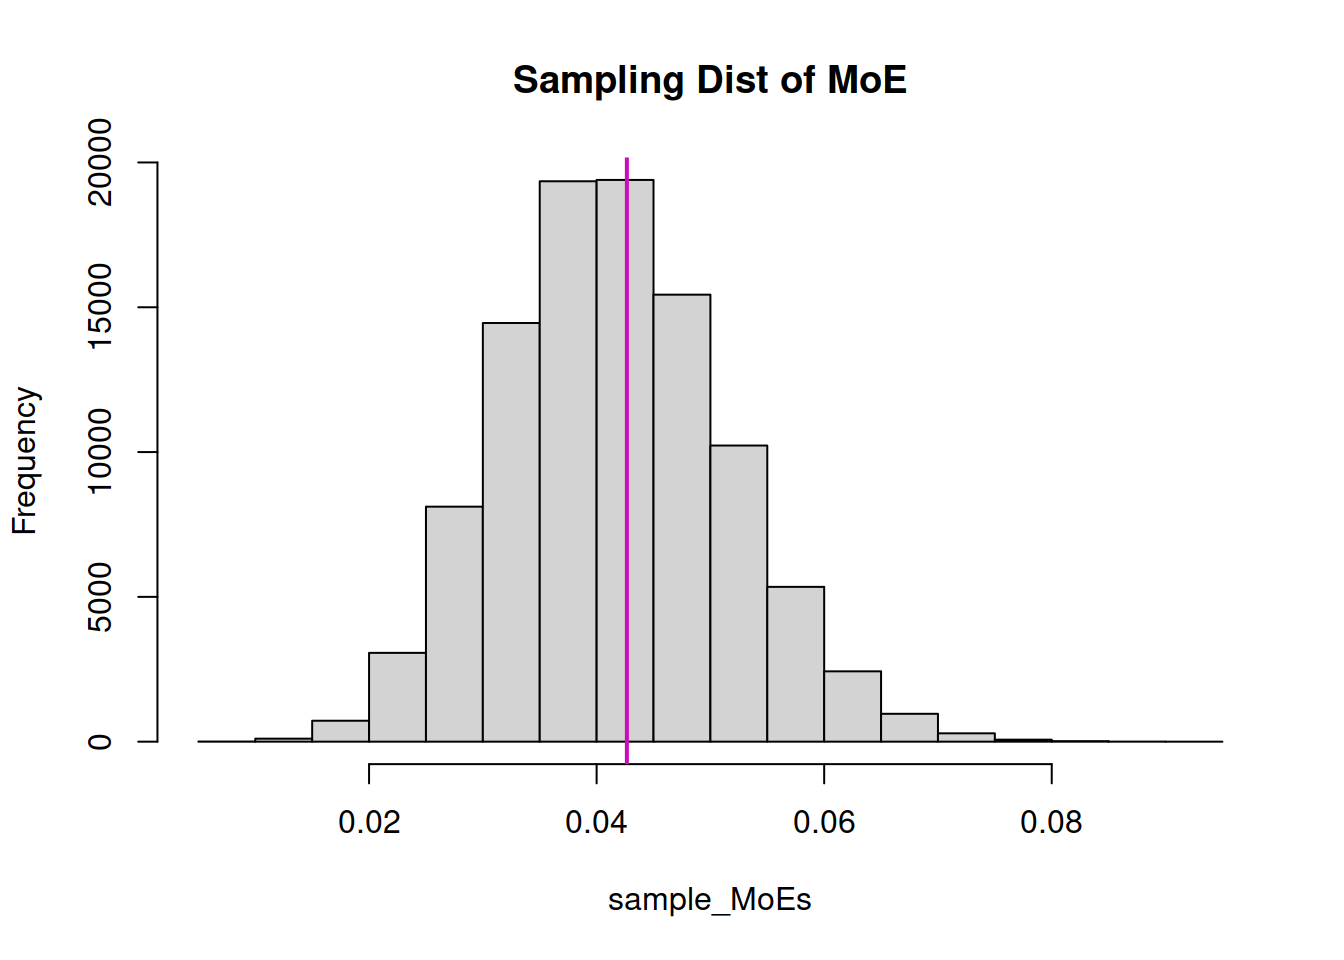
\includegraphics{L15-CI_for_Means_files/figure-pdf/sim_MoE-1.pdf}

}

\end{figure}

The vertical purple line is \(z^*\sigma/\sqrt n\).\footnote{Recall that
  this never changes since \(\sigma\) is fixed.} This is just a
re-scaling of the sampling distribution of the sample variance, so it's
also skewed! Furthermore, the average MoE using \(s\) is \emph{smaller}
than the MoE using \(\sigma\), even though it's right-skewed:

\begin{Shaded}
\begin{Highlighting}[]
\FunctionTok{c}\NormalTok{(}\StringTok{"MoE (sigma)"} \OtherTok{=}\NormalTok{ z\_star}\SpecialCharTok{*}\NormalTok{pop\_sd}\SpecialCharTok{/}\FunctionTok{sqrt}\NormalTok{(n),}
    \StringTok{"Average MoE (s)"} \OtherTok{=} \FunctionTok{mean}\NormalTok{(sample\_MoEs))}
\end{Highlighting}
\end{Shaded}

\begin{verbatim}
    MoE (sigma) Average MoE (s) 
     0.04265848      0.04148352 
\end{verbatim}

\begin{Shaded}
\begin{Highlighting}[]
\FunctionTok{c}\NormalTok{(}\StringTok{"MoE (sigma)"} \OtherTok{=}\NormalTok{ z\_star}\SpecialCharTok{*}\NormalTok{pop\_sd}\SpecialCharTok{/}\FunctionTok{sqrt}\NormalTok{(n),}
    \StringTok{"Median MoE (s)"} \OtherTok{=} \FunctionTok{median}\NormalTok{(sample\_MoEs))}
\end{Highlighting}
\end{Shaded}

\begin{verbatim}
   MoE (sigma) Median MoE (s) 
    0.04265848     0.04104300 
\end{verbatim}

This is why the CI using \(s\) doesn't capture the true mean as often -
it's giving us smaller intervals!

\hypertarget{removing-the-silliness}{%
\section{Removing the Silliness}\label{removing-the-silliness}}

The distribution of the sample variance is not important.\footnote{And
  very complicated.} Instead, we care about the confidence intervals.

I'm going to write this yet again: since
\(\bar X\sim N(\mu,\sigma/\sqrt{n})\)), \[
\frac{\bar X - \mu}{\sigma/\sqrt{n}} \sim N(0, 1)
\] That is, you take the sample means, subtract the mean of the means,
and divide by the \textbf{standard error}\footnote{the standard
  deviation of the sampling distribution}, and you get a standard normal
distribution.\footnote{The word ``standard'' shows up way too much.
  Statisticians are bad at naming things.}

On the other hand, if we use \(s\) (which has it's own variance), \[
\frac{\bar X - \mu}{s/\sqrt{n}} \sim t_{n-1}
\] where \(n-1\) is the \textbf{degrees of freedom} (or
\textbf{df}).\footnote{This is another example of statisticians being
  bad at naming things.} This is called the \(t\) distribution, and is a
lot like the normal distribution but it has higher variance.

Before we move on, notice how the formula with \(\sigma\) results in
N(0,1), which does not require any information for our sample. In the
\(t\) distribution, we need to know the sample size!

\hypertarget{the-t-distribution}{%
\subsection{The t distribution}\label{the-t-distribution}}

There are two main features of the \(t\) distribution that I want you to
know:

\begin{itemize}
\tightlist
\item
  It's centered at 0, just like N(0,1).
\item
  It's more variable than the normal distribution.
\end{itemize}

The second point is demonstrated in the following plot:

\includegraphics{L15-CI_for_Means_files/figure-pdf/unnamed-chunk-7-1.pdf}

The red line corresponds to a sample size of 2.\footnote{The degrees of
  freedom is \(n-1\).} As the colours move through red to blue, we
increase the sample size. At \(df = \infty\), the \(t\) distribution is
exactly the same as the N(0,1) distribution. For anything smaller, the
\(t\) distribution puts more probability in the tails.

This shows up in the critical values:

\begin{Shaded}
\begin{Highlighting}[]
\FunctionTok{abs}\NormalTok{(}\FunctionTok{qnorm}\NormalTok{(}\FloatTok{0.05}\SpecialCharTok{/}\DecValTok{2}\NormalTok{)) }\CommentTok{\# z\^{}*}
\end{Highlighting}
\end{Shaded}

\begin{verbatim}
[1] 1.959964
\end{verbatim}

\begin{Shaded}
\begin{Highlighting}[]
\FunctionTok{abs}\NormalTok{(}\FunctionTok{qt}\NormalTok{(}\FloatTok{0.05}\SpecialCharTok{/}\DecValTok{2}\NormalTok{, }\AttributeTok{df =} \DecValTok{15} \SpecialCharTok{{-}} \DecValTok{1}\NormalTok{)) }\CommentTok{\# t\^{}* n = 15}
\end{Highlighting}
\end{Shaded}

\begin{verbatim}
[1] 2.144787
\end{verbatim}

\begin{Shaded}
\begin{Highlighting}[]
\FunctionTok{abs}\NormalTok{(}\FunctionTok{qt}\NormalTok{(}\FloatTok{0.05}\SpecialCharTok{/}\DecValTok{2}\NormalTok{, }\AttributeTok{df =} \DecValTok{30} \SpecialCharTok{{-}} \DecValTok{1}\NormalTok{)) }\CommentTok{\# n = 30}
\end{Highlighting}
\end{Shaded}

\begin{verbatim}
[1] 2.04523
\end{verbatim}

\begin{Shaded}
\begin{Highlighting}[]
\FunctionTok{abs}\NormalTok{(}\FunctionTok{qt}\NormalTok{(}\FloatTok{0.05}\SpecialCharTok{/}\DecValTok{2}\NormalTok{, }\AttributeTok{df =} \DecValTok{50} \SpecialCharTok{{-}} \DecValTok{1}\NormalTok{)) }\CommentTok{\# n = 50}
\end{Highlighting}
\end{Shaded}

\begin{verbatim}
[1] 2.009575
\end{verbatim}

Note that, just like how \texttt{qbinom} finds the value such of a
binomial distribution such that 0.025\% of the distribution is to the
left and \texttt{qnorm} finds the z-values such that 0.025 is to the
left, \texttt{qt}\footnote{The person reading this is a cutie.} finds
the t-value.

\begin{Shaded}
\begin{Highlighting}[]
\NormalTok{n\_seq }\OtherTok{\textless{}{-}} \FunctionTok{seq}\NormalTok{(}\DecValTok{2}\NormalTok{, }\DecValTok{100}\NormalTok{, }\AttributeTok{by =} \DecValTok{2}\NormalTok{)}
\NormalTok{t\_seq }\OtherTok{\textless{}{-}} \FunctionTok{abs}\NormalTok{(}\FunctionTok{qt}\NormalTok{(}\FloatTok{0.05}\SpecialCharTok{/}\DecValTok{2}\NormalTok{, }\AttributeTok{df =}\NormalTok{ n\_seq}\DecValTok{{-}1}\NormalTok{))}
\FunctionTok{plot}\NormalTok{(n\_seq, t\_seq, }\AttributeTok{type =} \StringTok{"b"}\NormalTok{,}
    \AttributeTok{ylab =} \StringTok{"abs(qt(0.05/2, df = n {-} 1))"}\NormalTok{,}
    \AttributeTok{xlab =} \StringTok{"n"}\NormalTok{,}
    \CommentTok{\# the code for the title is not important.}
    \AttributeTok{main =} \FunctionTok{bquote}\NormalTok{(}\StringTok{"As df {-}\textgreater{} infinity, t"}\SpecialCharTok{\^{}}\StringTok{"*"}\SpecialCharTok{*}\StringTok{" {-}\textgreater{} z"}\SpecialCharTok{\^{}}\StringTok{"*"}\NormalTok{))}
\FunctionTok{abline}\NormalTok{(}\AttributeTok{h =} \FunctionTok{abs}\NormalTok{(}\FunctionTok{qnorm}\NormalTok{(}\FloatTok{0.05}\SpecialCharTok{/}\DecValTok{2}\NormalTok{)), }\AttributeTok{col =} \DecValTok{3}\NormalTok{, }\AttributeTok{lwd =} \DecValTok{2}\NormalTok{)}
\DocumentationTok{\#\# this code just puts a label on the axis {-} not important}
\FunctionTok{axis}\NormalTok{(}\DecValTok{2}\NormalTok{, }\FunctionTok{abs}\NormalTok{(}\FunctionTok{qnorm}\NormalTok{(}\FloatTok{0.05}\SpecialCharTok{/}\DecValTok{2}\NormalTok{)), }\StringTok{"z*"}\NormalTok{, }\AttributeTok{col =} \DecValTok{3}\NormalTok{, }\AttributeTok{font =} \DecValTok{2}\NormalTok{, }\AttributeTok{col.axis =} \DecValTok{3}\NormalTok{)}
\end{Highlighting}
\end{Shaded}

\begin{figure}[H]

{\centering \includegraphics{L15-CI_for_Means_files/figure-pdf/unnamed-chunk-9-1.pdf}

}

\end{figure}

Since there's more probability in the tails, you have to go further out
to find the point such that 0.025 of the distribution is to the
left.\footnote{Try this for other \(\alpha\) values and larger \(n\).}
The \(t\) distribution allows for more variance due to the variance of
\(s\), and it does this by having larger critical values.

\hypertarget{the-t-distribution-1}{%
\subsection{\texorpdfstring{The
\(t\)-distribution}{The t-distribution}}\label{the-t-distribution-1}}

The \(t\) distribution has higher variance than the Normal distribution
due to the extra uncertainty in estimating \(s\).

\hypertarget{the-t-confidence-interval}{%
\section{\texorpdfstring{The \(t\) Confidence
Interval}{The t Confidence Interval}}\label{the-t-confidence-interval}}

Now that you understand the reasoning behind using wider confidence
intervals, I can show you the formula/ \[
\bar x \pm t_{n-1}^*s/\sqrt{n}
\]

where \(t^*_{n-1}\) comes from
\texttt{abs(qt(alpha/2,\ df\ =\ n-1))}.\footnote{Note: I'm not even
  going to bother writing out the \(P()\) notation for \(t^*_{n-1}\)
  because you'll never use it. You'll only ever need to find
  \(t^*_{n-1}\) in this course.}

This has the same interpretation as the Z CI: 95\% of the intervals
constructed this way will contain the true population mean. This does
\textbf{NOT} mean that there's a 95\% chance that the interval contains
the true mean.

What's that? Of course, I can demonstrate by simulation! Thanks for
asking! The following code is copied and pasted from above, only the
critical value has been changed.

\begin{Shaded}
\begin{Highlighting}[]
\DocumentationTok{\#\# Set up empty vectors, to be filled with TRUE or FALSE}
\DocumentationTok{\#\# if the population mean is in the interval}
\NormalTok{sigma\_does }\OtherTok{\textless{}{-}} \FunctionTok{c}\NormalTok{() }\CommentTok{\# CI based on sigma does contain mu}
\NormalTok{s\_does }\OtherTok{\textless{}{-}} \FunctionTok{c}\NormalTok{() }\CommentTok{\# CI based on s does contain mu}

\NormalTok{pop\_sd }\OtherTok{\textless{}{-}} \DecValTok{1}
\NormalTok{pop\_mean }\OtherTok{\textless{}{-}} \DecValTok{0}
\NormalTok{n }\OtherTok{\textless{}{-}} \DecValTok{15} \CommentTok{\# sample size}

\NormalTok{z\_star }\OtherTok{\textless{}{-}} \FunctionTok{abs}\NormalTok{(}\FunctionTok{qnorm}\NormalTok{(}\FloatTok{0.05}\SpecialCharTok{/}\DecValTok{2}\NormalTok{))}
\NormalTok{t\_star }\OtherTok{\textless{}{-}} \FunctionTok{abs}\NormalTok{(}\FunctionTok{qt}\NormalTok{(}\FloatTok{0.05}\SpecialCharTok{/}\DecValTok{2}\NormalTok{, n }\SpecialCharTok{{-}} \DecValTok{1}\NormalTok{)) }\CommentTok{\# NEW}

\DocumentationTok{\#\# You aren\textquotesingle{}t expected to understand "for" loops, but}
\DocumentationTok{\#\# you need to be able to find CIs}
\ControlFlowTok{for}\NormalTok{(i }\ControlFlowTok{in} \DecValTok{1}\SpecialCharTok{:}\DecValTok{100000}\NormalTok{)\{ }\CommentTok{\# repeat this code a bunch of times}
\NormalTok{    new\_sample }\OtherTok{\textless{}{-}} \FunctionTok{rnorm}\NormalTok{(}\AttributeTok{n =}\NormalTok{ n, }\AttributeTok{mean =}\NormalTok{ pop\_mean, }\AttributeTok{sd =}\NormalTok{ pop\_sd)}
\NormalTok{    xbar }\OtherTok{\textless{}{-}} \FunctionTok{mean}\NormalTok{(new\_sample)}
\NormalTok{    samp\_sd }\OtherTok{\textless{}{-}} \FunctionTok{sd}\NormalTok{(new\_sample)}

\NormalTok{    CI\_sigma }\OtherTok{\textless{}{-}}\NormalTok{ xbar }\SpecialCharTok{+} \FunctionTok{c}\NormalTok{(}\SpecialCharTok{{-}}\DecValTok{1}\NormalTok{, }\DecValTok{1}\NormalTok{)}\SpecialCharTok{*}\NormalTok{z\_star}\SpecialCharTok{*}\NormalTok{pop\_sd}\SpecialCharTok{/}\FunctionTok{sqrt}\NormalTok{(n)}
\NormalTok{    CI\_s }\OtherTok{\textless{}{-}}\NormalTok{ xbar }\SpecialCharTok{+} \FunctionTok{c}\NormalTok{(}\SpecialCharTok{{-}}\DecValTok{1}\NormalTok{, }\DecValTok{1}\NormalTok{)}\SpecialCharTok{*}\NormalTok{t\_star}\SpecialCharTok{*}\NormalTok{samp\_sd}\SpecialCharTok{/}\FunctionTok{sqrt}\NormalTok{(n) }\CommentTok{\# NEW}
    \CommentTok{\# Do they contain the population mean?}
    \CommentTok{\# in other words, is the lower bound less than pop\_mean}
    \CommentTok{\# *and* is the upper bound larger than pop\_mean?}
    \CommentTok{\# (Not testable)}
\NormalTok{    sigma\_does[i] }\OtherTok{\textless{}{-}}\NormalTok{ (CI\_sigma[}\DecValTok{1}\NormalTok{] }\SpecialCharTok{\textless{}}\NormalTok{ pop\_mean) }\SpecialCharTok{\&}\NormalTok{ (CI\_sigma[}\DecValTok{2}\NormalTok{] }\SpecialCharTok{\textgreater{}}\NormalTok{ pop\_mean)}
\NormalTok{    s\_does[i] }\OtherTok{\textless{}{-}}\NormalTok{ (CI\_s[}\DecValTok{1}\NormalTok{] }\SpecialCharTok{\textless{}}\NormalTok{ pop\_mean) }\SpecialCharTok{\&}\NormalTok{ (CI\_s[}\DecValTok{2}\NormalTok{] }\SpecialCharTok{\textgreater{}}\NormalTok{ pop\_mean)}
\NormalTok{\}}

\DocumentationTok{\#\# The mean of a bunch of TRUEs and FALSEs is}
\DocumentationTok{\#\# the proportion of TRUEs (TRUE == 1, FALSE == 0)}
\FunctionTok{mean}\NormalTok{(sigma\_does)}
\end{Highlighting}
\end{Shaded}

\begin{verbatim}
[1] 0.95069
\end{verbatim}

\begin{Shaded}
\begin{Highlighting}[]
\FunctionTok{mean}\NormalTok{(s\_does)}
\end{Highlighting}
\end{Shaded}

\begin{verbatim}
[1] 0.95091
\end{verbatim}

Now both of them contain the mean 95\% of the time!\footnote{This means
  it's working!} The difference between them is that the t CI doesn't
have as much information as the Z CI - the Z CI knows what the
population sd is, but the t CI doesn't. This is kinda magical: using
math, we can get the truth with fewer assumptions!

\hypertarget{examples-5}{%
\section{Examples}\label{examples-5}}

\begin{enumerate}
\def\labelenumi{\arabic{enumi}.}
\tightlist
\item
  \(\bar x = 0.4\), \(n = 100\), \(\sigma = 0.01\), find the 92\%CI.

  \begin{itemize}
  \tightlist
  \item
    This is a bit of a trick: I gave you \(\sigma\)! This always refers
    to the population standard deviation, so that's what it is here. The
    Z CI can be found with the R code:
  \end{itemize}
\end{enumerate}

\begin{Shaded}
\begin{Highlighting}[]
\FloatTok{0.4} \SpecialCharTok{+} \FunctionTok{c}\NormalTok{(}\SpecialCharTok{{-}}\DecValTok{1}\NormalTok{, }\DecValTok{1}\NormalTok{)}\SpecialCharTok{*}\FunctionTok{abs}\NormalTok{(}\FunctionTok{qnorm}\NormalTok{(}\FloatTok{0.08}\SpecialCharTok{/}\DecValTok{2}\NormalTok{)) }\SpecialCharTok{*} \FloatTok{0.01}\SpecialCharTok{/}\FunctionTok{sqrt}\NormalTok{(}\DecValTok{100}\NormalTok{)}
\end{Highlighting}
\end{Shaded}

\begin{verbatim}
[1] 0.3982493 0.4017507
\end{verbatim}

\begin{enumerate}
\def\labelenumi{\arabic{enumi}.}
\setcounter{enumi}{1}
\tightlist
\item
  \(\bar x = 0.4\), \(n = 100\), \(s = 0.01\), will a 92\%CI be
  \emph{wider than} or \emph{smaller than} the CI from Example 1?

  \begin{itemize}
  \tightlist
  \item
    We use \(t\) to account for the extra variance we have when we
    estimate \(s\). More variance means wider tails! The CI will be
    wider!
  \end{itemize}
\end{enumerate}

\begin{Shaded}
\begin{Highlighting}[]
\FloatTok{0.4} \SpecialCharTok{+} \FunctionTok{c}\NormalTok{(}\SpecialCharTok{{-}}\DecValTok{1}\NormalTok{, }\DecValTok{1}\NormalTok{)}\SpecialCharTok{*}\FunctionTok{abs}\NormalTok{(}\FunctionTok{qt}\NormalTok{(}\FloatTok{0.08}\SpecialCharTok{/}\DecValTok{2}\NormalTok{, }\AttributeTok{df =} \DecValTok{100{-}1}\NormalTok{)) }\SpecialCharTok{*} \FloatTok{0.01}\SpecialCharTok{/}\FunctionTok{sqrt}\NormalTok{(}\DecValTok{100}\NormalTok{)}
\end{Highlighting}
\end{Shaded}

\begin{verbatim}
[1] 0.3982312 0.4017688
\end{verbatim}

It's only slightly wider. The sample size is large enough that the
variance in the estimate is small.\footnote{Recall: For both the sample
  mean and the sample proportion, the variance of the sampling
  distribution decreases as \(n\) increases.} Try this again with a
smaller \(n\) and see what happens to the difference!

\begin{enumerate}
\def\labelenumi{\arabic{enumi}.}
\setcounter{enumi}{2}
\tightlist
\item
  If \(n=16\) and the 95\%CI for \(\mu\) is (10, 15), what's the
  variance?

  \begin{enumerate}
  \def\labelenumii{\arabic{enumii}.}
  \tightlist
  \item
    A general form of the CI is \(\bar x \pm t^* s/\sqrt{n}\).

    \begin{itemize}
    \tightlist
    \item
      \(\bar x\) is in the centre, so \(\bar x\) is 12.5
    \end{itemize}
  \item
    The MoE is 2.5, so \(t^* s/\sqrt{n} = 2.5\).

    \begin{itemize}
    \tightlist
    \item
      \(t^*\) is \texttt{qt(0.05/2,\ 16\ -\ 1)} = 2.131
    \end{itemize}
  \item
    \(2.131s/\sqrt{16} = 2.5\), so \(s = 2.5\sqrt{16}/2.131 = 4.69\)
  \item
    The variance is \(4.69^2 = 21.9961\)
  \end{enumerate}
\end{enumerate}

\hypertarget{summary-6}{%
\section{Summary}\label{summary-6}}

This lesson could have been two sentences: The sample standard deviation
has variance, so each confidence interval based on \(s\) is slightly
different. To account for this, we use the \(t\) distribution. Then
again, when someone tells me their name at a party I immediately forget
it. Hopefully this long-winded exploration helps you understand why
these facts are true and how they're relevant to the course.

Note that all of the best practices for inference still apply! We can
still get smaller intervals by taking better samples with larger sample
sizes, and we still have to be careful to \emph{never} speak of a
calculated confidence interval in terms of chance.

The \(t\) confidence interval is actually used in practice. We'll see
some code that calculates the interval for us in the next lecture, and
then we'll never have to use \texttt{qt()} again! (Except possibly to
demonstrate knowledge on tests.)

\hypertarget{t-tests-for-a-mean}{%
\chapter{t-Tests for a Mean}\label{t-tests-for-a-mean}}

\hypertarget{when-we-use-s-we-use-t}{%
\section{\texorpdfstring{When we use \(s\), we use
\(t\)}{When we use s, we use t}}\label{when-we-use-s-we-use-t}}

We've been over this in confidence intervals, and the same thing applies
to hypothesis tests! If the population is normal (or the sample size is
large enough) and we have an SRS, then \[
\frac{\bar X - \mu}{s/\sqrt{n}}\sim t_{n-1}
\]

Again, the \(t\) distribution is used to account for the extra
variability from the estimated standard deviation.\footnote{Which is
  used in the caclulation of the Estimated Standard Error.}

This means our test statistic is \[
t_{obs} = \frac{\bar x - \mu}{s/\sqrt{n}}
\]

Since this is a \(t\) distibution, we use
\texttt{pt(t\_obs,\ df\ =\ n\ -1)}, possibly one minus and/or double,
depending on the alternate hypothesis.\footnote{Like \texttt{pnorm()},
  it always calculates the probability below the test statistic.}

That's it. That's the big difference. When we estimate the standard
deviation, we use the t-distribution.

\begin{tcolorbox}[enhanced jigsaw, toptitle=1mm, colbacktitle=quarto-callout-warning-color!10!white, breakable, leftrule=.75mm, left=2mm, opacityback=0, colframe=quarto-callout-warning-color-frame, rightrule=.15mm, toprule=.15mm, bottomtitle=1mm, titlerule=0mm, title=\textcolor{quarto-callout-warning-color}{\faExclamationTriangle}\hspace{0.5em}{The t-test for a population mean}, arc=.35mm, colback=white, bottomrule=.15mm, opacitybacktitle=0.6, coltitle=black]

Given a sample mean \(\bar x\) and a sample standard deviation \(s\),
our test statistic is: \[
t_{obs} = \frac{\bar x - \mu}{s/\sqrt{n}}
\] Our hypotheses and calculations of the p-value work the same as they
did for the z-test.

\end{tcolorbox}

\hypertarget{examples-6}{%
\section{Examples}\label{examples-6}}

\hypertarget{pilot-fatigue}{%
\subsection{Pilot Fatigue}\label{pilot-fatigue}}

In the pilot fatigue example from the Understanding p-values lecture, we
assumed that we had the population sd. I lied - it was actually a sample
statistic! We should have used a t-test, not a z test.

Recall:

\begin{itemize}
\tightlist
\item
  \(H_0: \mu = 15\) versus \(H_A: \mu > 15\) with
\item
  \(n = 16\), \(\bar x = 15.9\), \(s = 1.2\) (not \(\sigma\)) \[
  t_{obs} = \frac{15.9 - 15}{1.2/\sqrt{16}} = 3
  \]
\end{itemize}

Using the \(t\) distribution, our p-value is:

\begin{Shaded}
\begin{Highlighting}[]
\DecValTok{1} \SpecialCharTok{{-}} \FunctionTok{pt}\NormalTok{(}\DecValTok{3}\NormalTok{, }\AttributeTok{df =} \DecValTok{16}\NormalTok{)}
\end{Highlighting}
\end{Shaded}

\begin{verbatim}
[1] 0.00423975
\end{verbatim}

This is \emph{larger} than our previous p-value of 0.0013. This will
always be the case: if the \(z_{obs}\) test statistic is the same as the
\(t_{obs}\) test statistic, then the p-value for \(t_{obs}\) will be
wider.

\begin{tcolorbox}[enhanced jigsaw, toptitle=1mm, colbacktitle=quarto-callout-warning-color!10!white, breakable, leftrule=.75mm, left=2mm, opacityback=0, colframe=quarto-callout-warning-color-frame, rightrule=.15mm, toprule=.15mm, bottomtitle=1mm, titlerule=0mm, title=\textcolor{quarto-callout-warning-color}{\faExclamationTriangle}\hspace{0.5em}{p-values from a t-test are larger than a z-test (if you have
\(\sigma=s\))}, arc=.35mm, colback=white, bottomrule=.15mm, opacitybacktitle=0.6, coltitle=black]

We almost never know the population standard deviation, so we have extra
uncertainty. With extra uncertainty, we require more \emph{evidence}!
Recall that a p-value is a measure of evidence against a null.

\end{tcolorbox}

\hypertarget{matched-pairs}{%
\section{Matched Pairs}\label{matched-pairs}}

A matched pairs design allows us to use a one-sample t-test when it
looks like we have two samples\footnote{We'll learn about two-sample
  t-tests in the next lecture.}. Since the pairs are matched, we can
calculate the differences between pairs and treat this like a single
vector of observations. It is honkey tonk ridonkulous to say that we
know the true population standard deviation for the difference in
observations, so a \(z\) test could never be appropriate.

Consider the following example of a matched pairs experiment. Given a
sample of brave volounteers, we create a small cut on both hands and put
ointment on one of the two cuts\footnote{And most likely a bandage on
  both.}. This study design eliminates the variation in healing times
for different people since both cuts are on the same person! For each
individual, we observe a \emph{difference}. That is, one observation per
person!

\begin{longtable}[]{@{}lllllllll@{}}
\toprule\noalign{}
& Subject 1 & S2 & S3 & S4 & S5 & S6 & S7 & S8 \\
\midrule\noalign{}
\endhead
\bottomrule\noalign{}
\endlastfoot
With Ointment & 6.44 & 6.06 & 4.22 & 3.3 & 6.5 & 3.49 & 7.01 & 4.22 \\
Without & 7.22 & 6.05 & 4.55 & 4 & 6.7 & 2.88 & 7.88 & 6.32 \\
Difference & -0.78 & 0.01 & -0.33 & -0.7 & -0.2 & 0.61 & -0.87 & -2.1 \\
\end{longtable}

\emph{Note}: Differences were calculated as ``With minus Without''! This
will be important for setting up the alternative hypothesis later.

The important thing here is that last row of this table now represents
our data - we can forget that the other two rows exist! In other words,
we have \emph{one} observation per person, rather than two sets of
observations.

This is where the assumption that we know the population standard
deviation is especially preposterous: we're looking just at the
differences! Even if there's a true value of the sd for healing time for
all people, the standard deviation of the difference between healing
times isn't a reasonable quantity to speak of.

Since we're looking at the \emph{difference}, we no longer have a
hypothesized value of \(\mu_0\). Instead, we hypothesize that the
average pairwise difference is 0,
i.e.~\(\mu_{with\; minus\; without} = \mu_{diff} = 0\)\footnote{In other
  words, the healing times are the same for each subject}. The
alternative is ``with'' \textless{} ``without'',
i.e.~\(\mu_{diff} < 0\).\footnote{This is where it's important to know
  that we did ``with minus without''; we could have done without minus
  with, but then our alternate hypotheses would need to be
  ``\textgreater{}''.}

\begin{Shaded}
\begin{Highlighting}[]
\NormalTok{x }\OtherTok{\textless{}{-}} \FunctionTok{c}\NormalTok{(}\SpecialCharTok{{-}}\FloatTok{0.78}\NormalTok{, }\FloatTok{0.01}\NormalTok{, }\SpecialCharTok{{-}}\FloatTok{0.33}\NormalTok{, }\SpecialCharTok{{-}}\FloatTok{0.7}\NormalTok{, }\SpecialCharTok{{-}}\FloatTok{0.2}\NormalTok{, }\FloatTok{0.61}\NormalTok{, }\SpecialCharTok{{-}}\FloatTok{0.87}\NormalTok{, }\SpecialCharTok{{-}}\FloatTok{2.1}\NormalTok{)}
\NormalTok{xbar }\OtherTok{\textless{}{-}} \FunctionTok{mean}\NormalTok{(x)}
\NormalTok{s }\OtherTok{\textless{}{-}} \FunctionTok{sd}\NormalTok{(x)}
\NormalTok{n }\OtherTok{\textless{}{-}} \FunctionTok{length}\NormalTok{(x)}

\NormalTok{t\_obs }\OtherTok{\textless{}{-}}\NormalTok{ (xbar }\SpecialCharTok{{-}} \DecValTok{0}\NormalTok{)}\SpecialCharTok{/}\NormalTok{(s}\SpecialCharTok{/}\FunctionTok{sqrt}\NormalTok{(n)) }\CommentTok{\# xbar is with {-} w/out}
\CommentTok{\# Notice that we use pt() instead of pnorm()}
\FunctionTok{pt}\NormalTok{(t\_obs, }\AttributeTok{df =}\NormalTok{ n }\SpecialCharTok{{-}} \DecValTok{1}\NormalTok{) }\CommentTok{\# Alternative is \textless{}}
\end{Highlighting}
\end{Shaded}

\begin{verbatim}
[1] 0.04662624
\end{verbatim}

So our p-value is approximately 0.04. At the 5\% level, the null
hypothesis would be rejected and we would conclude that the ointment
works\footnote{A p-value says \emph{nothing} about the effect size, so
  we can't say whether it's \textbf{practically significant}}. At the
1\% level, we would conclude that it doesn't have a significant effect.
This is why it's important to know the significance level before
calculating the p-value - we shouldn't get to choose whether our results
are statistically significant!

\hypertarget{t-tests-in-practice}{%
\subsection{t-tests in Practice}\label{t-tests-in-practice}}

Do you think that researchers in the field are typing test statistics
into their calculator? Of course not! We're finally at the point in this
class where the methods are so commonly used that the built-in functions
in R can calculate them.

\begin{Shaded}
\begin{Highlighting}[]
\NormalTok{with\_oint }\OtherTok{\textless{}{-}} \FunctionTok{c}\NormalTok{(}\FloatTok{6.44}\NormalTok{, }\FloatTok{6.06}\NormalTok{, }\FloatTok{4.22}\NormalTok{, }\FloatTok{3.3}\NormalTok{, }\FloatTok{6.5}\NormalTok{, }\FloatTok{3.49}\NormalTok{, }\FloatTok{7.0}\NormalTok{, }\FloatTok{4.22}\NormalTok{)}
\NormalTok{without }\OtherTok{\textless{}{-}} \FunctionTok{c}\NormalTok{(}\FloatTok{7.22}\NormalTok{, }\FloatTok{6.05}\NormalTok{, }\FloatTok{4.55}\NormalTok{, }\DecValTok{4}\NormalTok{  , }\FloatTok{6.7}\NormalTok{, }\FloatTok{2.88}\NormalTok{, }\FloatTok{7.8}\NormalTok{, }\FloatTok{6.32}\NormalTok{)}
\NormalTok{difference }\OtherTok{\textless{}{-}}\NormalTok{ with\_oint }\SpecialCharTok{{-}}\NormalTok{ without}
\FunctionTok{t.test}\NormalTok{(difference, }\AttributeTok{alternative =} \StringTok{"less"}\NormalTok{)}
\end{Highlighting}
\end{Shaded}

\begin{verbatim}

    One Sample t-test

data:  difference
t = -1.9199, df = 7, p-value = 0.04817
alternative hypothesis: true mean is less than 0
95 percent confidence interval:
         -Inf -0.007063183
sample estimates:
mean of x 
 -0.53625 
\end{verbatim}

Notice that the output shows a \textbf{one-sided confidence interval}.
This isn't a big leap from what you know: a confidence interval consists
of all of the values that would \emph{not} be rejected by a hypothesis
test, and this works for one-sided as well as two-sided alternate
hypotheses!

To get a two-sided confidence interval, we can either leave
\texttt{alternative} at it's default value or set it to
\texttt{"two.sided"}. We can also change the significance level with the
\texttt{conf.level} argument. For an 89\%CI:

\begin{Shaded}
\begin{Highlighting}[]
\FunctionTok{t.test}\NormalTok{(difference, }\AttributeTok{alternative =} \StringTok{"two.sided"}\NormalTok{, }\AttributeTok{conf.level =} \FloatTok{0.89}\NormalTok{)}
\end{Highlighting}
\end{Shaded}

\begin{verbatim}

    One Sample t-test

data:  difference
t = -1.9199, df = 7, p-value = 0.09635
alternative hypothesis: true mean is not equal to 0
89 percent confidence interval:
 -1.04730428 -0.02519572
sample estimates:
mean of x 
 -0.53625 
\end{verbatim}

Notice that this calculated a two-sided p-value, which is twice what we
saw before (and no longer significant at the 5\% level!).

\hypertarget{recap-1}{%
\chapter{Recap}\label{recap-1}}

\hypertarget{hypothesis-tests-in-general}{%
\section{Hypothesis Tests in
General}\label{hypothesis-tests-in-general}}

\begin{enumerate}
\def\labelenumi{\arabic{enumi}.}
\tightlist
\item
  Decide on a hypothesis.

  \begin{itemize}
  \tightlist
  \item
    \(H_0: \mu = \mu_0\) versus
    \(H_a: \mu [\ne,>,\text{ or }<] \mu_0\)\lspace
  \end{itemize}
\item
  Choose a significance level \(\alpha\).

  \begin{itemize}
  \tightlist
  \item
    Smaller leverl = require more evidence to reject the null.\lspace
  \end{itemize}
\item
  Gather data

  \begin{itemize}
  \tightlist
  \item
    Independent observations from same population; random sample.\lspace
  \end{itemize}
\item
  Calculate the test statistic based on \(\bar x\), \(s\), and
  \(\mu_0\).

  \begin{itemize}
  \tightlist
  \item
    Sampling distribution is based on the \emph{null} hypothesis.\lspace
  \end{itemize}
\item
  Calculate the p-value according to the form of the \emph{alternate}
  hypothesis.

  \begin{itemize}
  \tightlist
  \item
    If \(<\), then \texttt{pnorm(z\_obs)}; if \(>\), then
    \texttt{1\ -\ pnorm(z\_obs)}; if two sided, double the correct one.
  \end{itemize}
\end{enumerate}

\hypertarget{hypothesis-test-example}{%
\section{Hypothesis Test Example}\label{hypothesis-test-example}}

New York is sometimes called ``the city that never sleeps''. At the 5\%
level, do the following data provide evidence that the average New
Yorker gets less than 8 hours of sleep per night?

\begin{longtable}[]{@{}lll@{}}
\toprule\noalign{}
\(\bar x\) & \(s\) & \(n\) \\
\midrule\noalign{}
\endhead
\bottomrule\noalign{}
\endlastfoot
7.73 & 0.77 & 25 \\
\end{longtable}

\begin{itemize}
\tightlist
\item
  Hypotheses: \pause \(H_0: \mu = 8\), \(H_a:\mu < 8\).\lspace
\item
  \(t_{obs}\) = \pause \(\dfrac{7.73 - 8}{0.77/5} = -1.75\)\lspace
\item
  p-value = \pause \texttt{pt(-1.75,\ 24)} = 0.0464
\item
  Conclude: \pause Since p \textless{} \(\alpha\), we reject the null
  hypothesis.

  \begin{itemize}
  \tightlist
  \item
    We have found statistically significant evidence that New Yorkers
    sleep less than 8 hours per night on average.
  \end{itemize}
\end{itemize}

\hypertarget{confidence-intervals-1}{%
\section{Confidence Intervals}\label{confidence-intervals-1}}

\begin{enumerate}
\def\labelenumi{\arabic{enumi}.}
\tightlist
\item
  Choose a confidence level \(\alpha\).

  \begin{itemize}
  \tightlist
  \item
    ``100(1-\(\alpha\))\%CI\lspace
  \end{itemize}
\item
  Collect data

  \begin{itemize}
  \tightlist
  \item
    Independent observations from same population; random sample.\lspace
  \end{itemize}
\item
  Find the critical value \(t^*_{n-1}\)

  \begin{itemize}
  \tightlist
  \item
    We will not need \(z^*\) again, except possibly as
    comparison.\lspace
  \end{itemize}
\item
  Calculate \(\bar x \pm t^*s/\sqrt{n}\)\lspace
\item
  Conclude: 95\% of the intervals constructed this way will contain the
  true population mean.
\end{enumerate}

\hypertarget{confidence-interval-example}{%
\section{Confidence Interval
Example}\label{confidence-interval-example}}

Construct a 95\% CI for the New York sleep example.

\begin{longtable}[]{@{}lll@{}}
\toprule\noalign{}
\(\bar x\) & \(s\) & \(n\) \\
\midrule\noalign{}
\endhead
\bottomrule\noalign{}
\endlastfoot
7.73 & 0.77 & 25 \\
\end{longtable}

\begin{itemize}
\tightlist
\item
  \(\alpha\) = \pause 0.05\lspace
\item
  \(t^*_{n-1}\) = \pause \texttt{qt(0.025,\ 24)} = -2.0639.\lspace
\item
  \(\bar x \pm t^*_{n-1}s/\sqrt{n} = 7.73 \pm 2.0639*0.77/5 = (7.41, 8.05)\)\lspace
\item
  Conclude: we are 95\% confident that the true average nights sleep in
  New York is between 7.41 and 8.05.

  \begin{itemize}
  \tightlist
  \item
    This interval includes 8, so 8 would \emph{not} be rejected by a
    hypothesis test?!?!
  \end{itemize}
\end{itemize}

\hypertarget{participation-questions-3}{%
\section{Participation Questions}\label{participation-questions-3}}

\hypertarget{q1-2}{%
\subsection{Q1}\label{q1-2}}

What is the standard error?

\pspace

\begin{enumerate}
\def\labelenumi{\arabic{enumi}.}
\tightlist
\item
  \(\sigma/\sqrt{n}\)
\item
  \(\sqrt{\frac{p(1-p)}{n}}\)
\item
  \(\sqrt{s_1^2/n_1 + s_2^2/n}\)
\item
  The standard deviation of the sampling distribution.
\end{enumerate}

\hypertarget{q2-2}{%
\subsection{Q2}\label{q2-2}}

What is the standard deviation of the sampling distribution?

\pspace

\begin{enumerate}
\def\labelenumi{\arabic{enumi}.}
\tightlist
\item
  The standard deviation of the population divided by the square root of
  the sample size (\(\sigma/\sqrt{n}\)).
\item
  The standard deviation of the value of a sample statistic across all
  possible samples from the population.
\item
  The same as the standard deviation of the population.
\item
  The average distance to the mean of the population.
\end{enumerate}

\hypertarget{q3-2}{%
\subsection{Q3}\label{q3-2}}

Why does the sampling distribution have a lower variance than the
population?

\pspace

\begin{enumerate}
\def\labelenumi{\arabic{enumi}.}
\tightlist
\item
  Because the standard deviation is smaller than the variance.
\item
  Because the population has a larger number of possible, so the
  variance is smaller.
\item
  Because outliers are not as likely in a sample.
\item
  Because we are summarising many observations from a sample into a
  single value.
\end{enumerate}

\hypertarget{q4-2}{%
\subsection{Q4}\label{q4-2}}

After conducting a study, we found a p-value of 0.04. Did we find a
statistically significant result?

\pspace

\begin{enumerate}
\def\labelenumi{\arabic{enumi}.}
\tightlist
\item
  Yes, since the p-value is less than 0.05
\item
  No, since the p-value is less than 0.05
\item
  We failed to set the significance lavel ahead of time, so we have to
  be very careful about concluding significance.
\end{enumerate}

\hypertarget{q5-2}{%
\subsection{Q5}\label{q5-2}}

After conducting a study, we found a 95\% confidence interval for
\(\mu\) from -0.1 to 1.9. What can we conclude?

\pspace

\begin{enumerate}
\def\labelenumi{\arabic{enumi}.}
\tightlist
\item
  Since 0 is in the interval, a hypothesis test for \(\mu = 0\) versus
  \(\mu \ne 0\) would not be significant at the 5\% level.
\item
  Since 0 is in the interval, a hypothesis test for \(\mu = 0\) versus
  \(\mu > 0\) would not be significant at the 5\% level.
\item
  Since 0 is in the interval, a hypothesis test for \(\mu = 0\) versus
  \(\mu \ne 0\) would not be significant at the 2.5\% level.
\item
  Since 0 is in the interval, a hypothesis test for \(\mu = 0\) versus
  \(\mu > 0\) would not be significant at the 2.5\% level.
\end{enumerate}

\hypertarget{q6-1}{%
\subsection{Q6}\label{q6-1}}

Under which condition does the CLT \emph{not} apply?

\pspace

\begin{enumerate}
\def\labelenumi{\arabic{enumi}.}
\tightlist
\item
  For \(\bar x\), the sample size is between 3 and 60 but a histogram of
  the sample appears normal.
\item
  For \(\bar x\), the sample size is much larger than 60.
\item
  For \(\hat p\), the sample size is much larger than 60.
\item
  For \(\hat p\), we have checked \(np>10\) and \(n(1-p)>10\)
\end{enumerate}

\hypertarget{self-study-questions-5}{%
\section{Self-Study Questions}\label{self-study-questions-5}}

\begin{enumerate}
\def\labelenumi{\arabic{enumi}.}
\tightlist
\item
  Explain why: If the \(z_{obs}\) test statistic is the same as the
  \(t_{obs}\) test statistic, then the p-value for \(t_{obs}\) will be
  wider.
\item
  If a test is statistically signficant, does that mean there's a large
  effect size? That is, does a hypothesis test tell you anything about
  the size of the effect?

  \begin{itemize}
  \tightlist
  \item
    Compare this to confidence intervals.
  \end{itemize}
\item
  Can we interpret a \(t\) confidence interval as ``all null hypothesis
  values that would not be rejected''?
\item
  Re-do the ointment example, but using without - with.

  \begin{enumerate}
  \def\labelenumii{\alph{enumii}.}
  \tightlist
  \item
    Draw a t distribution and mark the two test statistics, then fill in
    the area that corresponds to the p-value.
  \end{enumerate}
\end{enumerate}

\hypertarget{two-sample-t-tests}{%
\chapter{Two-Sample t-Tests}\label{two-sample-t-tests}}

\hypertarget{how-much-can-one-more-sample-complicate-things}{%
\section{How much can one more sample complicate
things?}\label{how-much-can-one-more-sample-complicate-things}}

\hypertarget{notation-subscripts-everywhere}{%
\subsection{Notation: Subscripts
everywhere!}\label{notation-subscripts-everywhere}}

We now have two samples.

\(\bar X_1\sim N(\mu_1, \sigma_1/\sqrt{n_1})\), where \(s_1\) is the
estimated standard deviation of a given sample.

\(\bar X_2\sim N(\mu_2, \sigma_2/\sqrt{n_2})\) \pause

\quad

\emph{Goal:} Are the means the same? I.e., is \(\mu_1 = \mu_2\)?

With two samples, the difference in means has a sampling distribution.
What is that distribution? It's difficult!

The easy part is the mean of the difference. The mean of the difference
is the difference in means. \[
\bar X_1 - \bar X_2 \sim N(\mu_1 - \mu_2, ???)
\]

The hard part is the standard deviation of the difference. Take a moment
and think about what we're talking about here. What does it actually
mean for the difference in means to have variance?

It's the same as it was before, it just seems a little more complicated.
When we take a pair of samples then find their difference, we have
calculated a statistic! For every \emph{pair} of samples, we'll get a
different statistic. The variance that we seek is the variance of all of
these statistics.

\hypertarget{the-standard-deviation-of-a-difference}{%
\subsection{The standard deviation of a
difference}\label{the-standard-deviation-of-a-difference}}

Again, I'm going to use a simulation to demonstrate what happens if we
take a bunch of pairs of samples, then find their difference.

In this case, I'm sampling x1 as 22 values from a normal distribution
with a mean of 0 and a standard deviation of 2, whereas x2 has 33
observations and comes from a distribution with a mean of 0 and a
standard deviation of 3. I'm finding their means, then finding their
differences. I repeat this 10,000 times, keeping track of what the
difference in means was.

\begin{Shaded}
\begin{Highlighting}[]
\DocumentationTok{\#\# approximating the sampling distribution}
\NormalTok{differences }\OtherTok{\textless{}{-}} \FunctionTok{c}\NormalTok{()}
\ControlFlowTok{for}\NormalTok{(i }\ControlFlowTok{in} \DecValTok{1}\SpecialCharTok{:}\DecValTok{10000}\NormalTok{)\{}
\NormalTok{    m1 }\OtherTok{\textless{}{-}} \FunctionTok{mean}\NormalTok{(}\FunctionTok{rnorm}\NormalTok{(}\DecValTok{22}\NormalTok{, }\DecValTok{0}\NormalTok{, }\DecValTok{2}\NormalTok{))}
\NormalTok{    m2 }\OtherTok{\textless{}{-}} \FunctionTok{mean}\NormalTok{(}\FunctionTok{rnorm}\NormalTok{(}\DecValTok{33}\NormalTok{, }\DecValTok{0}\NormalTok{, }\DecValTok{3}\NormalTok{))}
\NormalTok{    differences[i] }\OtherTok{\textless{}{-}}\NormalTok{ m1 }\SpecialCharTok{{-}}\NormalTok{ m2}
\NormalTok{\}}
\FunctionTok{sd}\NormalTok{(differences)}
\end{Highlighting}
\end{Shaded}

\begin{verbatim}
[1] 0.6802144
\end{verbatim}

\ldots{} it's not at all obvious where this number comes from.

Both had a mean of 0, so the difference should be 0. But the standard
deviation of the differences isn't obvious. There is a nice formula for
the mean - \(\sigma/\sqrt{n}\) - but it's not obvious how this works for
two samples with different variances \emph{and} different sample sizes!

It turns out that the following equation is the correct one for the
standard deviation of the differences. Recall that the standard
deviation of a sampling distribution is known as the Standard Error
(SE).

\[
SE = \sqrt{\frac{s_1^2}{n_1} + \frac{s_2^2}{n_2}}
\]

And to verify that our simulation matches this idea:

\begin{Shaded}
\begin{Highlighting}[]
\DocumentationTok{\#\# Check}
\FunctionTok{sd}\NormalTok{(differences)}
\end{Highlighting}
\end{Shaded}

\begin{verbatim}
[1] 0.6802144
\end{verbatim}

\begin{Shaded}
\begin{Highlighting}[]
\FunctionTok{sqrt}\NormalTok{(}\DecValTok{4}\SpecialCharTok{/}\DecValTok{22} \SpecialCharTok{+} \DecValTok{9}\SpecialCharTok{/}\DecValTok{33}\NormalTok{) }\CommentTok{\# Close enough}
\end{Highlighting}
\end{Shaded}

\begin{verbatim}
[1] 0.6741999
\end{verbatim}

\hypertarget{putting-it-together}{%
\subsection{Putting it Together}\label{putting-it-together}}

Altogether, this means that the difference between means has the
following sampling distribution:

\[
\bar X_1 - \bar X_2 \sim N\left(\mu_1 - \mu_2, \sqrt{\frac{s_1^2}{n_1} + \frac{s_2^2}{n_2}}\right)
\]

From this, we get the same general ideas as before. The hypothesis tests
are based on the observed test statistic: \[
t_{obs} = \frac{\text{sample statistic} - \text{hypothesized value}}{\text{standard error}} = \frac{(\bar x_1 - \bar x_2) - 0}{\sqrt{\frac{s_1^2}{n_1} + \frac{s_2^2}{n_2}}}
\] where usually the hypothesized value is 0 so that we're testing
whether the true population means are the same.

\hypertarget{two-sample-hypotheses}{%
\subsection{Two-Sample Hypotheses}\label{two-sample-hypotheses}}

The usual hypotheses invlove the \emph{equality} of the means, i.e.:
\begin{align*}
H_0: \mu_1 = \mu_2 &\Leftrightarrow H_0:\mu_1 - \mu_2 = \mu_d = 0\\
H_0: \mu_1 < \mu_2 &\Leftrightarrow H_0:\mu_1 - \mu_2 = \mu_d < 0\\
\end{align*}

The confidence interval is also the same idea: \[
\text{sample statistic}\pm\text{critical value}*\text{standard error} = (\bar x_1 - \bar x_2)\pm t^*\sqrt{\frac{s_1^2}{n_1} + \frac{s_2^2}{n_2}}
\]

In both of these, we still need to know the degrees of freedom! As we
saw last lecture, the \(t\)-distribution requires some information about
the sample size. In the one sample case, this was \(n-1\). However, we
now have two potentially different sample sizes! What do we do?

Recall that the \(t\)-distribution gets closer and closer to the normal
distribution as \(n\) increases. The whole point of the \(t\) is to get
us a little further from the normal in order to account for the variance
in the sample standard deviation. For the two-sample case, there is a
``correct'' formula, but it's big and scary and everything we're doing
now is approximate anyway. Instead, we use a more conservative approach
to ensure that we're not underestimating the variance.\footnote{In
  general, we would much, much, much rather \emph{overestimate} the
  variance. The whole point of statistics is to avoid overconfidence in
  our estimates.}

\hypertarget{two-sample-t-degrees-of-freedom}{%
\subsection{\texorpdfstring{Two-Sample \(t\) degrees of
freedom}{Two-Sample t degrees of freedom}}\label{two-sample-t-degrees-of-freedom}}

We use the smallest sample size, then subtract 1.

In the simulation we did earlier, the two samples had sizes of 22 and
33. In both a CI and a hypothesis test, we would use 21 as the value in
\texttt{qt()} or \texttt{pt()} (which are the same idea as
\texttt{qnorm()} and \texttt{pnorm()}).

\hypertarget{aside-pooled-variance}{%
\subsection{Aside: ``Pooled Variance''}\label{aside-pooled-variance}}

There's another formula out there that uses a so-called ``pooled
variance'' for the standard error of the differences. This assumes that
both populations have the exact same variance, and tries to use
information from both to estimate the variance. It essentially treats
the two samples as one big sample from the same population in order to
calculate the standard deviation.

This also implicitly assumes that both populations are normal, and this
is not based on the CLT. Instead, the populations need to be normal.
This is a huge assumption - we can use normality from the CLT because
the math checks out. Assuming normality of the population is just a wild
guess that we can't really check.

It is also very, very unlikely that the two populations have the same
standard deviation.

If the two assumptions are met, then the pooled standard deviation is
the ``correct'' formula. However, the SE that we saw before still works
very well! If the assumptions are not met, then the pooled SE works
poorly and the SE we've seen is still very good!

Except in exceptional cases, the SE that we've learned should be used.
The idea of a pooled variance is a vestige of another age.

\hypertarget{summary-7}{%
\section{Summary}\label{summary-7}}

\hypertarget{two-sample-t-test-and-ci-overview}{%
\subsection{Two-Sample t-test and CI
Overview}\label{two-sample-t-test-and-ci-overview}}

We are usually testing for the difference in means, i.e. \begin{align*}
H_0: \mu_1 = \mu_2 &\Leftrightarrow H_0:\mu_1 - \mu_2 = \mu_d = 0\\
H_a: \mu_1 < \mu_2 &\Leftrightarrow H_a:\mu_1 - \mu_2 = \mu_d < 0\\
\end{align*}\vspace{-15mm}

\[
t_{obs} = \frac{\bar x_1 - \bar x_2}{\sqrt{\frac{s_1^2}{n_1} + \frac{s_2^2}{n_2}}}
\] \vspace{-10mm}

\[
\text{p-value} = P(T < t_{obs}) = \texttt{pt(t\_obs, df = min(n1, n2) - 1)}
\]

\[
\text{A $(1-\alpha)$ CI for $\mu_d$ is }\bar x_1 - \bar x_2 \pm t^*\sqrt{\frac{s_1^2}{n_1} + \frac{s_2^2}{n_2}}
\]

where \(t^*\) is based on the smaller of \(n_1 - 1\) and \(n_2 - 1\)

\hypertarget{examples-7}{%
\section{Examples}\label{examples-7}}

\hypertarget{example-1-two-sample-versus-matched}{%
\subsection{Example 1: Two-Sample versus
Matched}\label{example-1-two-sample-versus-matched}}

From the Ointment example:

\begin{longtable}[]{@{}lllllllll@{}}
\toprule\noalign{}
& Subject 1 & S2 & S3 & S4 & S5 & S6 & S7 & S8 \\
\midrule\noalign{}
\endhead
\bottomrule\noalign{}
\endlastfoot
With Oint & 6.44 & 6.06 & 4.22 & 3.3 & 6.5 & 3.49 & 7.01 & 4.22 \\
Without & 7.22 & 6.05 & 4.55 & 4 & 6.7 & 2.88 & 7.88 & 6.32 \\
Difference & -0.78 & 0.01 & -0.33 & -0.7 & -0.2 & 0.61 & -0.87 & -2.1 \\
\end{longtable}

First we'll do matched pairs. In this example, this is the correct test
to use.

\begin{Shaded}
\begin{Highlighting}[]
\NormalTok{withoint }\OtherTok{\textless{}{-}} \FunctionTok{c}\NormalTok{(}\FloatTok{6.44}\NormalTok{, }\FloatTok{6.06}\NormalTok{, }\FloatTok{4.22}\NormalTok{, }\FloatTok{3.3}\NormalTok{, }\FloatTok{6.5}\NormalTok{, }\FloatTok{3.49}\NormalTok{, }\FloatTok{7.01}\NormalTok{, }\FloatTok{4.22}\NormalTok{)}
\NormalTok{without }\OtherTok{\textless{}{-}} \FunctionTok{c}\NormalTok{(}\FloatTok{7.22}\NormalTok{, }\FloatTok{6.05}\NormalTok{, }\FloatTok{4.55}\NormalTok{, }\DecValTok{4}\NormalTok{, }\FloatTok{6.7}\NormalTok{, }\FloatTok{2.88}\NormalTok{, }\FloatTok{7.88}\NormalTok{, }\FloatTok{6.32}\NormalTok{)}
\NormalTok{diff }\OtherTok{\textless{}{-}}\NormalTok{ withoint }\SpecialCharTok{{-}}\NormalTok{ without}

\FunctionTok{t.test}\NormalTok{(}\AttributeTok{x =}\NormalTok{ diff, }\AttributeTok{alternative =} \StringTok{"less"}\NormalTok{)}
\end{Highlighting}
\end{Shaded}

\begin{verbatim}

    One Sample t-test

data:  diff
t = -1.9421, df = 7, p-value = 0.04663
alternative hypothesis: true mean is less than 0
95 percent confidence interval:
        -Inf -0.01332314
sample estimates:
mean of x 
   -0.545 
\end{verbatim}

We could instead have done a two-sample test, which ignores the fact
that the observations are paired. Since we know the pairings, this test
is leaving out valuable information.

\begin{Shaded}
\begin{Highlighting}[]
\FunctionTok{t.test}\NormalTok{(}\AttributeTok{x =}\NormalTok{ withoint, }\AttributeTok{y =}\NormalTok{ without, }\AttributeTok{alternative =} \StringTok{"less"}\NormalTok{)}
\end{Highlighting}
\end{Shaded}

\begin{verbatim}

    Welch Two Sample t-test

data:  withoint and without
t = -0.67584, df = 13.736, p-value = 0.2552
alternative hypothesis: true difference in means is less than 0
95 percent confidence interval:
      -Inf 0.8772719
sample estimates:
mean of x mean of y 
    5.155     5.700 
\end{verbatim}

This result should not be trusted since it misses a key aspect of the
data.

\hypertarget{example-2-body-mass-of-penguins}{%
\subsection{Example 2: Body Mass of
Penguins}\label{example-2-body-mass-of-penguins}}

In this example, we'll look at the difference in body mass between male
and female penguins.

In this case, there is no clear pairing between the penguins. If they
were monogomous couples, then the differences in body mass might tell us
about couples, but doesn't say much about male and female penguins in
general.

This example gives us the opportunity to learn more notation in R! The
previous example used \texttt{t.test(x=...,\ y=...)} to denote the two
samples. If the data are neatly formatted in a data frame, then we can
use the \texttt{\textasciitilde{}} notation to demonstrate that the body
mass is split into different groups for male and female:

\begin{Shaded}
\begin{Highlighting}[]
\FunctionTok{library}\NormalTok{(palmerpenguins)}
\FunctionTok{t.test}\NormalTok{(body\_mass\_g }\SpecialCharTok{\textasciitilde{}}\NormalTok{ sex, }\AttributeTok{data =}\NormalTok{ penguins)}
\end{Highlighting}
\end{Shaded}

\begin{verbatim}

    Welch Two Sample t-test

data:  body_mass_g by sex
t = -8.5545, df = 323.9, p-value = 4.794e-16
alternative hypothesis: true difference in means between group female and group male is not equal to 0
95 percent confidence interval:
 -840.5783 -526.2453
sample estimates:
mean in group female   mean in group male 
            3862.273             4545.685 
\end{verbatim}

From this output, we get a two-sided p-value as well as a two-sided CI,
both confirming that the difference in body mass is different from 0.
You can also see that it's using ``female minus male'', rather than
``male minus female''. This is because R will put them in alphabetical
order, so female comes first.

You may also be happy to hear that no, you will never have to manually
enter the standard error formula! You may need to interpret it for
tests, though!

\hypertarget{conclusion-1}{%
\section{Conclusion}\label{conclusion-1}}

\begin{itemize}
\tightlist
\item
  If you can have matched pairs, you should use a matched pairs test.
\item
  Most of the time, you'll need to use a two-sample t-test.

  \begin{itemize}
  \tightlist
  \item
    Don't get fooled by equal sample sizes!
  \end{itemize}
\item
  A two-sample t-test is based on the difference in means

  \begin{itemize}
  \tightlist
  \item
    The standard error is tricky.
  \item
    The degrees of freedom is the \emph{smallest} sample size minus 1.

    \begin{itemize}
    \tightlist
    \item
      Used for the p-value for hypothesis tests and the critical value
      for confidence intervals.
    \end{itemize}
  \item
    The null hypothesis is usually 0, and the alternate dependes on the
    order in which you subtract the means.
  \end{itemize}
\end{itemize}

\hypertarget{two-sample-t-test-example}{%
\section{Two Sample t-test Example}\label{two-sample-t-test-example}}

Do mothers who smoke give birth to children with a lower birthweight
than mothers who don't?

\pspace

Test this at the 5\% level using the data on the right.

\vspace{-7mm}

\begin{longtable}[]{@{}lll@{}}
\toprule\noalign{}
& Smoker & Non-Smoker \\
\midrule\noalign{}
\endhead
\bottomrule\noalign{}
\endlastfoot
mean & 6.78 & 7.18 \\
sd & 1.43 & 1.60 \\
n & 50 & 100 \\
\end{longtable}

\begin{itemize}
\tightlist
\item
  The null hypothesis is \(H_0: \mu_{smoke} = \mu_{non}\), which can be
  written as
  \(H_0: \mu_{non} - \mu_{smoke} = \mu_{n - s} = 0\).\pause\lspace
\item
  The alternate hypothesis is \(H_a: \mu_{smoke} < \mu_{non}\), which
  could be written as

  \begin{itemize}
  \tightlist
  \item
    \(H_a: \mu_{n - s} > 0\), or
  \item
    \(H_a: \mu_{s - n} < 0\)
  \end{itemize}
\end{itemize}

It doesn't matter which we choose, but we have to calculate the
corresponding p-value! Let's use \(\mu_{n-s}\).

The sample mean difference is \(\bar x_{n - s} = 7.18 - 6.78 = 0.4\).
The standard error is: \[
SE = \sqrt{\dfrac{s_s^2}{n_s} + \dfrac{s_n^2}{n_n}} = \sqrt{\dfrac{1.43^2}{50} + \dfrac{1.60^2}{100}} = 0.2578721
\]

Since we used \(\bar x_{n - s}\), our alternate tells us to find the
p-value for a t-statistic larger than what we got.

\[
t_{obs} = \dfrac{\bar x_{n-s} - \mu_{n-s}}{SE} = \dfrac{0.4 - 0}{0.2578721} = 1.55
\]

Since we're doing a right-tailed test, we calculate our p-value as:

\begin{Shaded}
\begin{Highlighting}[]
\DecValTok{1} \SpecialCharTok{{-}} \FunctionTok{pt}\NormalTok{(}\FloatTok{1.55}\NormalTok{, }\DecValTok{49}\NormalTok{)}
\end{Highlighting}
\end{Shaded}

\begin{verbatim}
[1] 0.06378844
\end{verbatim}

To summarise:

\begin{itemize}
\tightlist
\item
  \(H_0: \mu_{n - s} = 0\) versus \(H_0: \mu_{n - s} > 0\)
\item
  \(t_{obs} = 1.55\)
\item
  p-value is 0.06
\end{itemize}

Since our p-value is larger than 0.5, we do not have a statistically
significant result. We fail to reject the hypothesis that smokers have
lower birthweights. We conclude that we do not have enough evidence to
say that smoking is associated with lower birthweights.

\hypertarget{large-sample-test-for-a-proportion}{%
\chapter{Large sample test for a
proportion}\label{large-sample-test-for-a-proportion}}

\hypertarget{refresher}{%
\section{Refresher}\label{refresher}}

In the lecture on sampling distributions, we learned that the sampling
distribution of a sample proportion can be found as follows:

If \(X\sim B(n,p)\) and \(np>10\) and \(n(1-p)>10\), then \[
\hat p \sim N\left(p, \sqrt{\frac{p(1-p)}{n}}\right)
\]

This relies on the population proportion to find the standard error, but
this is never available.\footnote{If it was, then why are we doing
  inference?}

\hypertarget{hypothesis-tests-for-proportions}{%
\section{Hypothesis tests for
proportions}\label{hypothesis-tests-for-proportions}}

As before, we write our hypotheses: \[
H_0:p = p_0 \text{ vs. } H_A: p \{>or<or\ne\} p_0
\]

We always write \(H_0:p = p_0\) and then fill in the value for \(p_0\),
then we use that same value in the alternate hypothesis but use either
\(>\), \(<\), or \(\ne\) based on the wording of the question.

As before, we use the sampling distribution to find our p-value. In this
case, though, we have a hypothesized value for the population
proportion. In fact, we \emph{must} assume that the null is
true.\footnote{We want to be strict about this so that it's more
  convincing if we prove it wrong.} If this is the case, we \emph{do
have} the standard error!

I swear, this is the last time I introduce a new standard error for the
sampling distribution of the sample proportion.\footnote{I'm lying.}
Assuming \(H_0\) is true (and the conditions are met), \[
\hat p \sim N\left(p_0, \sqrt{\frac{p_0(1-p_0)}{n}}\right)
\]

\hypertarget{the-test-statistic}{%
\subsection{The Test Statistic}\label{the-test-statistic}}

As you can guess from the sampling distribution, the test statistic is:

\begin{tcolorbox}[enhanced jigsaw, toptitle=1mm, colbacktitle=quarto-callout-note-color!10!white, breakable, leftrule=.75mm, left=2mm, opacityback=0, colframe=quarto-callout-note-color-frame, rightrule=.15mm, toprule=.15mm, bottomtitle=1mm, titlerule=0mm, title=\textcolor{quarto-callout-note-color}{\faInfo}\hspace{0.5em}{Test Statistic for a Test for Proportions}, arc=.35mm, colback=white, bottomrule=.15mm, opacitybacktitle=0.6, coltitle=black]

\[
z_{obs} = \frac{\text{observed} - \text{hypothesized}}{\text{standard error}} = \frac{\hat p - p_0}{\sqrt{p_0(1-p_0)/n}}
\]

\end{tcolorbox}

and then we can use the normal distribution as usual: \[
P(Z \{>or<or\text{ further away than}\} z_{obs}) = \dots
\]

where we use \(>\) if the alternate hypothesis uses \(>\), \(<\) if the
alternate hypothesis uses \(<\), and we look at the two tails if the
alternate hypothesis is \(\ne\).

A common question is: which \(p\) do we use to check normality? We're
supposed to check \(np\) and \(n(1-p)\), but do we use \(\hat p\) or
\(p_0\)?

For a hypothesis test, we assume the null is true, i.e.~\(p=p_0\). We
should use this assumption \emph{everywhere}! For a hypothesis test
about a proportion, we check whether \(np_0>10\) and
\(n(1-p_0)>10\)\footnote{As before, both conditions must be true; it's
  not enough for just \(np_0>10\) alone.}.

From here, we proceed as usual. We check the observed test statistic
against a \emph{normal} distribution and see whether our data are too
extreme to come from the distribution assumed in the null hypothesis.

\hypertarget{example-3}{%
\section{Example}\label{example-3}}

\hypertarget{mendelian-genetics}{%
\subsection{Mendelian Genetics}\label{mendelian-genetics}}

To test his theory that 75\% of plants would inheret a dominant gene,
Gregor Mendel cross bred pure breeds of pea plants. Out of 7324 plants,
5474 showed the dominant trait. At the 4.5\% level, is this compatible
with the hypothesis of 75\% dominant?

\textbf{Solution:}

\begin{enumerate}
\def\labelenumi{\arabic{enumi}.}
\tightlist
\item
  Check: \(np_0 = 7324*0.75 > 10\) and \(n(1-p_0) = 7324*0.25 > 10\).
\item
  \(z_{obs} = \frac{\hat p - p_0}{\sqrt{p_0(1-p_0)/n}} = \frac{0.747 - 0.75}{\sqrt{0.75*0.25/7324}} = -0.513\)
\item
  \(p-val = 2 *P(Z < z_{obs})\) = \texttt{2*pnorm(-0.513)} = 0.608

  \begin{itemize}
  \tightlist
  \item
    We doubled the \(P(Z < z_{obs})\) because we want both tails. If you
    do this and your p-value is larger than 1, do \(1 - P(Z < z_{obs})\)
    first and then double it.
  \end{itemize}
\item
  Conclusion: Since \(p-val > \alpha\), we do not reject the null. The
  hypothesis that 75\% of plants inherent the dominant trait is
  compatible with the data.
\end{enumerate}

The last step is important: always word your conclusion in the context
of the study.

These methods are extremely widespread, so of course they're implemented
in R. Here's a verification of our results:

\begin{Shaded}
\begin{Highlighting}[]
\FunctionTok{prop.test}\NormalTok{(}\AttributeTok{x =} \DecValTok{5474}\NormalTok{, }\AttributeTok{n =} \DecValTok{7324}\NormalTok{, }\AttributeTok{p =} \FloatTok{0.75}\NormalTok{)}
\end{Highlighting}
\end{Shaded}

\begin{verbatim}

    1-sample proportions test with continuity correction

data:  5474 out of 7324, null probability 0.75
X-squared = 0.24923, df = 1, p-value = 0.6176
alternative hypothesis: true p is not equal to 0.75
95 percent confidence interval:
 0.7372578 0.7572926
sample estimates:
        p 
0.7474058 
\end{verbatim}

The output should look familiar - it's very similar to the t-test
output.

We can see that the p-value (be careful not to mix up the
\texttt{p-value} and the estimate of \(p\), labelled \texttt{p} - these
are very different things!) is a little different. Maybe it's because of
rounding errors? We calculated the z test statistic to the nearest 3
decimal places, maybe that wasn't enough?

\begin{Shaded}
\begin{Highlighting}[]
\NormalTok{x }\OtherTok{\textless{}{-}} \DecValTok{5474}
\NormalTok{n }\OtherTok{\textless{}{-}} \DecValTok{7324}
\NormalTok{phat }\OtherTok{\textless{}{-}}\NormalTok{ x }\SpecialCharTok{/}\NormalTok{ n}
\NormalTok{se }\OtherTok{\textless{}{-}} \FunctionTok{sqrt}\NormalTok{(}\FloatTok{0.75} \SpecialCharTok{*}\NormalTok{ (}\DecValTok{1} \SpecialCharTok{{-}} \FloatTok{0.75}\NormalTok{) }\SpecialCharTok{/}\NormalTok{ n)}
\DecValTok{2}\SpecialCharTok{*}\FunctionTok{pnorm}\NormalTok{((phat }\SpecialCharTok{{-}} \FloatTok{0.75}\NormalTok{) }\SpecialCharTok{/}\NormalTok{ se)}
\end{Highlighting}
\end{Shaded}

\begin{verbatim}
[1] 0.6081484
\end{verbatim}

Nope, it's not a rounding problem!

The actual answer is that R uses a \emph{continuity correction factor}
(which isn't going to be on the test for this course). The correction
factor ``shifts'' the data so that the normal distribution aligns with
the center of the bar, rather than the edge. See the following plot for
why.

\includegraphics{L18-Hypothesis_Tests_for_Proportions_files/figure-pdf/unnamed-chunk-3-1.pdf}

As you can see, the normal distribution aligns with the side of the bar.
For values below the mean (in this case, \(n=10\) and \(p=0.4\), so the
mean is 4), the normal distribution is overestimating the areas to the
left, whereas above the mean it's underestimating the areas to the left.
The correction factor shifts the normal distribution to the right by 0.5
so that it's a better estimate of the areas below the curve.

If we run \texttt{prop.test()} without the correction factor, we get the
exact same p-value that we saw before.

\begin{Shaded}
\begin{Highlighting}[]
\FunctionTok{prop.test}\NormalTok{(}\AttributeTok{x =} \DecValTok{5474}\NormalTok{, }\AttributeTok{n =} \DecValTok{7324}\NormalTok{, }\AttributeTok{p =} \FloatTok{0.75}\NormalTok{, }\AttributeTok{correct =} \ConstantTok{FALSE}\NormalTok{)}
\end{Highlighting}
\end{Shaded}

\begin{verbatim}

    1-sample proportions test without continuity correction

data:  5474 out of 7324, null probability 0.75
X-squared = 0.26288, df = 1, p-value = 0.6081
alternative hypothesis: true p is not equal to 0.75
95 percent confidence interval:
 0.7373269 0.7572253
sample estimates:
        p 
0.7474058 
\end{verbatim}

These details are not important, just be aware that almost all tests for
proportions are run \emph{with} the continuity correction factor.

\hypertarget{mendelian-genetics-confidence-interval}{%
\subsection{Mendelian Genetics Confidence
Interval}\label{mendelian-genetics-confidence-interval}}

Recall from last lecture the duality of the CI and the hypothesis test.
For this question, a 95.5\%\footnote{\(\alpha = 0.045\), so
  \(1 - \alpha = 0.955\).}

In order to find the confidence interval, we again need the standard
error! In the hypothesis test, we assumed that \(p_0\) was the true
population proportion in order to proceed with the test. However, we
don't make this assumption for confidence intervals.

What can we do? We don't have \(p\) or \(p_0\), so we're left with
\(\hat p\), the sample proportion that we calculated. In the t-test,
this meant that we needed to switch to the \(t\) distribution. However,
that was because there was really good theory to say that the \(t\)
distribution is the correct distribution to use. There's no such theory
here.

\begin{tcolorbox}[enhanced jigsaw, toptitle=1mm, colbacktitle=quarto-callout-warning-color!10!white, breakable, leftrule=.75mm, left=2mm, opacityback=0, colframe=quarto-callout-warning-color-frame, rightrule=.15mm, toprule=.15mm, bottomtitle=1mm, titlerule=0mm, title=\textcolor{quarto-callout-warning-color}{\faExclamationTriangle}\hspace{0.5em}{CIs for Proportions Only Work When the CLT Applies}, arc=.35mm, colback=white, bottomrule=.15mm, opacitybacktitle=0.6, coltitle=black]

The \(t\)-distribution allows us to do hypothesis tests and make CIs
even for smaller samples when we're not sure that the CLT applies. For
proportions, we need a ``large'' sample.

\end{tcolorbox}

Now that we know all this, the CI can be found as: \[
\hat p \pm z^*\sqrt{\frac{\hat p(1-\hat p)}{n}} = 0.747 \pm 2.005\sqrt{\frac{0.747(1-0.747)}{7324}}
\]

which results in the CI (0.737, 0.758). This matches the CI shown in the
output of \texttt{prop.test()} above (double check this!).

\begin{tcolorbox}[enhanced jigsaw, toptitle=1mm, colbacktitle=quarto-callout-warning-color!10!white, breakable, leftrule=.75mm, left=2mm, opacityback=0, colframe=quarto-callout-warning-color-frame, rightrule=.15mm, toprule=.15mm, bottomtitle=1mm, titlerule=0mm, title=\textcolor{quarto-callout-warning-color}{\faExclamationTriangle}\hspace{0.5em}{Duality of Hypotheses and CIs}, arc=.35mm, colback=white, bottomrule=.15mm, opacitybacktitle=0.6, coltitle=black]

For proportions, it is \emph{not} true that the CI contains all
hypotheses that would not be rejected because the CI and the hypothesis
test use different standard errors.

\end{tcolorbox}

\hypertarget{exact-test-for-binomial}{%
\section{Exact Test for Binomial}\label{exact-test-for-binomial}}

In this course, we use the normal approximation to the binomial in order
to do hypothesis tests. This is not the only way to do it: we don't
always need to use the approximation! There's something called the
``exact binomial test'', which is a hypothesis test that uses the
binomial distribution rather than the normal approximation (this will
not be on tests).

There are two main reasons why we might prefer the approximation, rather
than using the exact test:

\begin{enumerate}
\def\labelenumi{\arabic{enumi}.}
\tightlist
\item
  If we have a large sample, then the approximation and the exact test
  are very very close. The approximation is computationally simpler.

  \begin{itemize}
  \tightlist
  \item
    If we have a small sample, neither tests can accurately approximate
    the variance of the population, and thus the estimated standard
    error isn't well estimated either.
  \end{itemize}
\item
  Because the binomial distribution is discrete, the p-values for many
  different test statistics will be the same. By setting \(\alpha\), we
  might not actually be getting \(\alpha\).

  \begin{itemize}
  \tightlist
  \item
    This is a technical point that can be safely ignored when studying
    for tests.
  \end{itemize}
\end{enumerate}

The exact test can be performed using the \texttt{binom.test()} function
in R.

\hypertarget{summary-8}{%
\section{Summary}\label{summary-8}}

CIs and Hypothesis Tests work exactly as they did before, but now we're
dealing with proportions. Just like the change from one sample to two
sample \(t\) tests, the standard error is important and difficult.

\begin{itemize}
\tightlist
\item
  For hypothesis tests, the standard error uses \(p_0\).
\item
  For CIs, the standard error uses \(\hat p\).
\end{itemize}

Interpreting these confidence intervals and hypothesis tests is very
similar to before, but you must keep in mind that they're proportions.
This mainly affects how you describe the end results.

There are two other wrinkles to consider when using proportions:

\begin{itemize}
\tightlist
\item
  The default test for proportions is the normal approximation with
  continuity correction.

  \begin{itemize}
  \tightlist
  \item
    It is possible, but not recommended, to not use continuity
    correction.
  \end{itemize}
\item
  There is also an exact test, but for large samples the approximation
  is faster and easier.
\end{itemize}

\hypertarget{self-study-questions-6}{%
\section{Self-Study Questions}\label{self-study-questions-6}}

\begin{enumerate}
\def\labelenumi{\arabic{enumi}.}
\tightlist
\item
  When do we use \(\hat p\) in the standard error? When do we use
  \(p_0\)?
\item
  Explain why we don't estimate the standard error in a hypothesis test
  about a proportion.
\item
  Explain in your own words why there's no \(t\) version of a hypothesis
  test for proportions.
\item
  Write a good summary of the Mendelian genetics example. What did we
  conclude, and how is this knowledge useful?
\end{enumerate}

\hypertarget{confidence-intervals-for-a-proportion}{%
\chapter{Confidence Intervals for a
Proportion}\label{confidence-intervals-for-a-proportion}}

\hypertarget{introduction-6}{%
\section{Introduction}\label{introduction-6}}

\hypertarget{this-is-the-same-as-the-last-video.}{%
\subsection{This is the same as the last
video.}\label{this-is-the-same-as-the-last-video.}}

\begin{itemize}
\item
  Based on our data, we make an interval that we think describes the
  population.\newline\pause
\item
  In this case, we just have a different population distribution?
\end{itemize}

\hypertarget{assumptions}{%
\subsection{Assumptions}\label{assumptions}}

In stats, assumptions give us power \pause but only if they hold.

\pause

Assumptions for a CI for \(p\) are the same as the assumptions for the
binomial distribution, with the addition of an SRS.

\hypertarget{the-ci-for-p}{%
\section{\texorpdfstring{The CI for
\(p\)}{The CI for p}}\label{the-ci-for-p}}

\hypertarget{sampling-distribution-of-hat-p}{%
\subsection{\texorpdfstring{Sampling Distribution of
\(\hat p\)}{Sampling Distribution of \textbackslash hat p}}\label{sampling-distribution-of-hat-p}}

As we saw before the midterm, if the population is \(B(n,p)\), then
under certain conditions,

\[\hat p \sim N\left(p, \sqrt{\frac{p(1-p)}{n}}\right)\]

\hypertarget{deja-vu}{%
\subsection{Deja-Vu}\label{deja-vu}}

Since \(\hat p \sim N(p, \sqrt{\frac{p(1-p)}{n}})\),

\[
\frac{\hat p - p}{\sqrt{p(1-p)/n}} \sim N(0,1)
\]

\pause Again, we can use the form \(z = (x-\mu)/\sigma\), but replace
\(x\), \(\mu\), and \(\sigma\) with the correct values.\pause

A \((1-\alpha)\)CI for \(p\) is:

\[
\hat p \pm z^*\sqrt{\frac{p(1-p)}{n}}
\]

\hypertarget{we-dont-know-the-variance-why-not-t_n-1}{%
\subsection{\texorpdfstring{We don't know the variance, why not
\(t_{n-1}^*\)?}{We don't know the variance, why not t\_\{n-1\}\^{}*?}}\label{we-dont-know-the-variance-why-not-t_n-1}}

\begin{itemize}
\item
  We used \(t_{n-1}^*\) because we had to estimate \(\sigma\)\newline
\item
  There's no \(\sigma\) to estimate!\newline
\item
  The variance of the Binomial distribution is entirely determined by
  \(p\)!

  \begin{itemize}
  \tightlist
  \item
    Binom be crazy.
  \end{itemize}
\end{itemize}

\hypertarget{but-devan-we-still-dont-know-p}{%
\subsection{\texorpdfstring{\ldots{} but Devan, we still don't know
\(p\)!}{\ldots{} but Devan, we still don't know p!}}\label{but-devan-we-still-dont-know-p}}

The \((1-\alpha)\)CI for \(p\) is:

\[
\hat p \pm z^*\sqrt{\frac{p(1-p)}{n}}
\] which needs \(p\) in the second part of the equation.\pause

\quad

Why not just plug in \(\hat p\)?\pause

Okay fine. \pause

\(\sqrt{\hat p(1-\hat p)/n}\) is called the \textbf{estimated standard
error}, since its the sd of the sampling distribution, but it's based on
an estimate.

\hypertarget{final_version_v2_update_lasttry_srsly.docx.pdf}{%
\subsection{Final\_Version\_V2\_Update\_LastTry\_Srsly.docx.pdf}\label{final_version_v2_update_lasttry_srsly.docx.pdf}}

The \((1-\alpha)\)CI for \(p\) is:

\[
\hat p \pm z^*\sqrt{\frac{\hat p(1-\hat p)}{n}}
\]

where \(z^*\) is chosen such that \(P(Z < -z^*) = \alpha/2\).

\hypertarget{devan-style-simulation}{%
\subsection{Devan Style: Simulation}\label{devan-style-simulation}}

\begin{Shaded}
\begin{Highlighting}[]
\NormalTok{n }\OtherTok{\textless{}{-}} \DecValTok{100}
\NormalTok{p }\OtherTok{\textless{}{-}} \FloatTok{0.7}
\NormalTok{SE\_true }\OtherTok{\textless{}{-}} \FunctionTok{sqrt}\NormalTok{(p}\SpecialCharTok{*}\NormalTok{(}\DecValTok{1}\SpecialCharTok{{-}}\NormalTok{p)}\SpecialCharTok{/}\NormalTok{n)}
\NormalTok{p\_does }\OtherTok{\textless{}{-}} \FunctionTok{c}\NormalTok{()}
\NormalTok{phat\_does }\OtherTok{\textless{}{-}} \FunctionTok{c}\NormalTok{()}
\NormalTok{that\_does }\OtherTok{\textless{}{-}} \FunctionTok{c}\NormalTok{()}
\NormalTok{z\_star }\OtherTok{\textless{}{-}} \FunctionTok{abs}\NormalTok{(}\FunctionTok{qnorm}\NormalTok{(}\FloatTok{0.05}\SpecialCharTok{/}\DecValTok{2}\NormalTok{))}
\NormalTok{t\_star }\OtherTok{\textless{}{-}} \FunctionTok{abs}\NormalTok{(}\FunctionTok{qt}\NormalTok{(}\FloatTok{0.05}\SpecialCharTok{/}\DecValTok{2}\NormalTok{, }\AttributeTok{df =}\NormalTok{ n}\DecValTok{{-}1}\NormalTok{))}
\end{Highlighting}
\end{Shaded}

\hypertarget{devan-style-simulation-1}{%
\subsection{Devan Style: Simulation}\label{devan-style-simulation-1}}

\begin{Shaded}
\begin{Highlighting}[]
\ControlFlowTok{for}\NormalTok{(i }\ControlFlowTok{in} \DecValTok{1}\SpecialCharTok{:}\DecValTok{10000}\NormalTok{)\{}
\NormalTok{    new\_sample }\OtherTok{\textless{}{-}} \FunctionTok{rbinom}\NormalTok{(}\AttributeTok{n=}\DecValTok{1}\NormalTok{, }\AttributeTok{size=}\NormalTok{n, }\AttributeTok{prob=}\NormalTok{p)}
\NormalTok{    phat }\OtherTok{\textless{}{-}}\NormalTok{ new\_sample}\SpecialCharTok{/}\NormalTok{n}
\NormalTok{    SE\_est }\OtherTok{\textless{}{-}} \FunctionTok{sqrt}\NormalTok{(phat}\SpecialCharTok{*}\NormalTok{(}\DecValTok{1}\SpecialCharTok{{-}}\NormalTok{phat)}\SpecialCharTok{/}\NormalTok{n)}
    
\NormalTok{    pCI }\OtherTok{\textless{}{-}}\NormalTok{ phat }\SpecialCharTok{+} \FunctionTok{c}\NormalTok{(}\SpecialCharTok{{-}}\DecValTok{1}\NormalTok{,}\DecValTok{1}\NormalTok{)}\SpecialCharTok{*}\NormalTok{z\_star}\SpecialCharTok{*}\NormalTok{SE\_true}
\NormalTok{    phatCI }\OtherTok{\textless{}{-}}\NormalTok{ phat }\SpecialCharTok{+} \FunctionTok{c}\NormalTok{(}\SpecialCharTok{{-}}\DecValTok{1}\NormalTok{,}\DecValTok{1}\NormalTok{)}\SpecialCharTok{*}\NormalTok{z\_star}\SpecialCharTok{*}\NormalTok{SE\_est}
\NormalTok{    thatCI }\OtherTok{\textless{}{-}}\NormalTok{ phat }\SpecialCharTok{+} \FunctionTok{c}\NormalTok{(}\SpecialCharTok{{-}}\DecValTok{1}\NormalTok{,}\DecValTok{1}\NormalTok{)}\SpecialCharTok{*}\NormalTok{t\_star}\SpecialCharTok{*}\NormalTok{SE\_est}
    
\NormalTok{    p\_does[i] }\OtherTok{\textless{}{-}}\NormalTok{ pCI[}\DecValTok{1}\NormalTok{] }\SpecialCharTok{\textless{}}\NormalTok{ p }\SpecialCharTok{\&}\NormalTok{ pCI[}\DecValTok{2}\NormalTok{] }\SpecialCharTok{\textgreater{}}\NormalTok{ p}
\NormalTok{    phat\_does[i] }\OtherTok{\textless{}{-}}\NormalTok{ phatCI[}\DecValTok{1}\NormalTok{] }\SpecialCharTok{\textless{}}\NormalTok{ p }\SpecialCharTok{\&}\NormalTok{ phatCI[}\DecValTok{2}\NormalTok{] }\SpecialCharTok{\textgreater{}}\NormalTok{ p}
\NormalTok{    that\_does[i] }\OtherTok{\textless{}{-}}\NormalTok{ thatCI[}\DecValTok{1}\NormalTok{] }\SpecialCharTok{\textless{}}\NormalTok{ p }\SpecialCharTok{\&}\NormalTok{ thatCI[}\DecValTok{2}\NormalTok{] }\SpecialCharTok{\textgreater{}}\NormalTok{ p}
\NormalTok{\}}
\end{Highlighting}
\end{Shaded}

\hypertarget{simulation-results}{%
\subsection{Simulation Results}\label{simulation-results}}

\begin{Shaded}
\begin{Highlighting}[]
\FunctionTok{mean}\NormalTok{(p\_does)}
\end{Highlighting}
\end{Shaded}

\begin{verbatim}
[1] 0.9371
\end{verbatim}

\begin{Shaded}
\begin{Highlighting}[]
\FunctionTok{mean}\NormalTok{(phat\_does)}
\end{Highlighting}
\end{Shaded}

\begin{verbatim}
[1] 0.9502
\end{verbatim}

\begin{Shaded}
\begin{Highlighting}[]
\FunctionTok{mean}\NormalTok{(that\_does)}
\end{Highlighting}
\end{Shaded}

\begin{verbatim}
[1] 0.9502
\end{verbatim}

Using the population proportion is\ldots{} worse?\pause

DIY: Change \(p\) so that the normal approximation doesn't apply.

\hypertarget{examlpes-and-cautions}{%
\section{Examlpes and Cautions}\label{examlpes-and-cautions}}

\hypertarget{example-1-1}{%
\subsection{Example 1}\label{example-1-1}}

It was found that 591 out of 700 people sampled supported a certain
political position. Find a 91\%CI.

\hypertarget{example-2-1}{%
\subsection{Example 2}\label{example-2-1}}

It was found that 68 out of 70 people sampled supported a certain
political position. Find a 91\%CI.\pause

\begin{Shaded}
\begin{Highlighting}[]
\NormalTok{n }\OtherTok{\textless{}{-}} \DecValTok{70}
\NormalTok{phat }\OtherTok{\textless{}{-}} \DecValTok{68}\SpecialCharTok{/}\DecValTok{70}
\NormalTok{se\_est }\OtherTok{\textless{}{-}} \FunctionTok{sqrt}\NormalTok{(phat}\SpecialCharTok{*}\NormalTok{(}\DecValTok{1}\SpecialCharTok{{-}}\NormalTok{phat)}\SpecialCharTok{/}\NormalTok{n)}
\NormalTok{z\_star }\OtherTok{\textless{}{-}} \FunctionTok{abs}\NormalTok{(}\FunctionTok{qnorm}\NormalTok{(}\FloatTok{0.09}\SpecialCharTok{/}\DecValTok{2}\NormalTok{))}

\NormalTok{phat }\SpecialCharTok{+} \FunctionTok{c}\NormalTok{(}\SpecialCharTok{{-}}\DecValTok{1}\NormalTok{, }\DecValTok{1}\NormalTok{)}\SpecialCharTok{*}\NormalTok{z\_star}\SpecialCharTok{*}\NormalTok{se\_est}
\end{Highlighting}
\end{Shaded}

\begin{verbatim}
[1] 0.9376692 1.0051879
\end{verbatim}

\ldots{} so it would be reasonable to say that the popluation proportion
is larger than 1???

\hypertarget{example-2-2}{%
\subsection{Example 2}\label{example-2-2}}

It was found that 68 out of 70 people sampled supported a certain
political position. Find a 91\%CI.\pause

\begin{Shaded}
\begin{Highlighting}[]
\FunctionTok{prop.test}\NormalTok{(}\AttributeTok{x =} \DecValTok{68}\NormalTok{, }\AttributeTok{n =} \DecValTok{70}\NormalTok{)}
\end{Highlighting}
\end{Shaded}

\begin{verbatim}

    1-sample proportions test with continuity correction

data:  68 out of 70, null probability 0.5
X-squared = 60.357, df = 1, p-value = 7.912e-15
alternative hypothesis: true p is not equal to 0.5
95 percent confidence interval:
 0.8913981 0.9950358
sample estimates:
        p 
0.9714286 
\end{verbatim}

\hypertarget{inference-for-the-difference-in-proportions}{%
\chapter{Inference for the Difference in
Proportions}\label{inference-for-the-difference-in-proportions}}

\hypertarget{diy-confidence-intervals}{%
\section{DIY Confidence Intervals}\label{diy-confidence-intervals}}

This lesson is going to be a little different from the rest. I'm not
going to give you the answers, I'm going to give you the tools.

\hypertarget{standard-error-for-a-single-mean}{%
\subsection{Standard Error for a Single
Mean}\label{standard-error-for-a-single-mean}}

As we've seen many times, this is \[
SE(\bar X) = \frac{\sigma}{\sqrt{n}} = \sqrt{\frac{\sigma^2}{n}},
\] but we often use \[
\hat{SE}(\bar X) = \frac{S}{\sqrt{n}} = \sqrt{\frac{S^2}{n}},
\] which is the \textbf{estimated standard error} (the ``hat'' on top of
the letters ``SE'' indicates that it's estimated). For the rest of this
lecture, we'll always use the estimated standard error.

\hypertarget{standard-error-for-the-difference-in-means}{%
\subsection{Standard Error for the Difference in
Means}\label{standard-error-for-the-difference-in-means}}

Even though we were subtracting means, we added their variances and then
take their square root. \[
\hat{SE}(\bar X_1 - \bar X_2) = \sqrt{\frac{s_1^2}{n_1} + \frac{s_2^2}{n_2}}
\] It is an important fact that we add the variances and then take the
square root.

From this lesson, also note that we had to make the assumptions:

\begin{itemize}
\tightlist
\item
  The individuals within a group are independent of other individuals in
  that group.

  \begin{itemize}
  \tightlist
  \item
    For example, if we sample people in our own family then the samples
    are not independent. People in the same family tend to have similar
    characteristics, so knowledge of the characteristics of one family
    member are informative about the others.\footnote{Recall that
      \textbf{independence} means that knowledge of one outcome gives
      you a better guess at other outcomes.}
  \end{itemize}
\item
  The \emph{groups} are independent.

  \begin{itemize}
  \tightlist
  \item
    For example, if we're looking at the difference in mean heights
    between men and women, but we have spousal pairs. Spousal pairs have
    a smaller difference in height than the average difference in
    height.\footnote{In this example, we could find the difference in
      heights between spouses, then use this collection of differences
      in a \emph{one-sample} t-test, which gives us different
      information, but it's also interesting.}
  \end{itemize}
\end{itemize}

\hypertarget{standard-error-for-a-single-proportion}{%
\subsection{Standard Error for a Single
Proportion}\label{standard-error-for-a-single-proportion}}

This is nothing new, I'm just repeating it here: \[
\hat{SE}(\hat p) = \sqrt{\frac{\hat p(1 - \hat p)}{n}}
\]

\hypertarget{standard-error-for-the-difference-in-proportions}{%
\subsection{Standard Error for the Difference in
Proportions}\label{standard-error-for-the-difference-in-proportions}}

This is up to you to find! Keed these in mind:

\begin{itemize}
\tightlist
\item
  The standard error cannot be negative, so you probably can't subtract
  things.
\item
  Variances can be added if we assume things are independent.

  \begin{itemize}
  \tightlist
  \item
    Make these assumptions explicit!
  \end{itemize}
\end{itemize}

\hypertarget{confidence-interval-example-1}{%
\subsection{Confidence Interval
Example}\label{confidence-interval-example-1}}

This question is from \emph{OpenIntro Introductory Statistics for the
Life and Biomedical Sciences, First Edition}.

The way a question is phrased can influence a person's response. For
example, Pew Research Center conducted a survey with the following
question:

\begin{quote}
As you may know, by 2014 nearly all Americans will be required to have
health insurance. {[}People who do not buy insurance will pay a
penalty{]} while {[}People who cannot afford it will receive financial
help from the government{]}. Do you approve or disapprove of this
policy?
\end{quote}

For each randomly sampled respondent, the statements in brackets were
randomized: either they were kept in the order given above, or the order
of the two statements was reversed. The table below shows the results of
this experiment. Calculate and interpret a 90\% confidence interval of
the difference in the probability of approval of the policy.

\begin{longtable}[]{@{}lll@{}}
\toprule\noalign{}
& Sample size \(n_i\) & Approve \% \\
\midrule\noalign{}
\endhead
\bottomrule\noalign{}
\endlastfoot
Original Ordering & 771 & 47 \\
Reversed Ordering & 732 & 34 \\
\end{longtable}

\textbf{Solution}

Let \(p_1\) be the proportion who approve when given the original
ordering with sample size \(n_1\), and \(p_2\) be the proportion who
approve when given the reversed ordering with sample size \(n_2\). This
question is asking us to calculate a confidence interval for
\(p_1 - p_2\).

We first check the conditions required to use the normal approximation.

\begin{enumerate}
\def\labelenumi{\arabic{enumi}.}
\tightlist
\item
  Pew Research Center is basically the world expert on opinion polling,
  so the samples are probably good.
\item
  We can safely assume that the samples are independent.
\item
  The two statements were randomly assigned, so it's safe to say that
  the two groups are independent.
\item
  \(n_1 * 0.47 = 771 * 0.47 = 362.37\)

  \begin{itemize}
  \tightlist
  \item
    There are \emph{three} other calculations to check. Check them!
  \end{itemize}
\end{enumerate}

Now that that's covered, we can make a confidence interval. The general
form is: \[
\text{Point Estimate}\pm\text{Critical Value}*\text{Standard Error}
\] From your homework above, verify that you can calculate the standard
error as 0.025.\footnote{This is to ensure you have the correct
  caclulation, you won't need to do this on a test.}

Our point estimate is \(\hat p_1 - \hat p_2 = 0.47 - 0.34 = 0.13\).
Since we doing a difference in proportions, our critical value comes
from the normal distribution:

\begin{Shaded}
\begin{Highlighting}[]
\FunctionTok{qnorm}\NormalTok{((}\DecValTok{1} \SpecialCharTok{{-}} \FloatTok{0.9}\NormalTok{)}\SpecialCharTok{/}\DecValTok{2}\NormalTok{)}
\end{Highlighting}
\end{Shaded}

\begin{verbatim}
[1] -1.644854
\end{verbatim}

So our confidence interval is: \[
0.13 \pm 1.65*0.025 = (0.09, 0.17)
\]

We are 90\% confident that the true mean difference is between 0.09 and
0.17. This provides evidence that the two proportions are indeed
different.

\hypertarget{hypothesis-testing}{%
\section{Hypothesis Testing}\label{hypothesis-testing}}

Here's where things are a little less obvious - I'm not going to get you
to find the standard error yourself!

We are generally looking at a hypothesis test for whether two
proportions are \emph{equal}, that is, \[
H_0: p_1 = p_2\implies p_1 - p_2 = 0
\] with an alternative that they are not equal, or that one is bigger
than the other. In other words, we're looking at the
hypotheses:\footnote{There may be a time in your life where you test
  whether \(p_1 - p_2 = 0.25\) or something like that, and you'll need
  to modify the methods a little bit.} \begin{align*}
H_0: &p_{1-2} = 0\\
H_A: &p_{1-2} \ne 0\text{ or }p_{1-2} > 0\text{ or }p_{1-2} > 0\\
\end{align*}

In the lesson on proportions, we saw that the standard error depended on
the null hypothesis being \emph{true}, since we calculate p-values under
the assumption that the null hypothesis is true. How do we do that here?

\hypertarget{the-pooled-proportion}{%
\subsection{The Pooled Proportion}\label{the-pooled-proportion}}

Under the null hypothesis, \(p_1 = p_2\). That's like saying that we
observed a bunch of successes and failures from a single group, instead
of two. Let \(x_1\) be the number of successes in the first group, and
\(x_2\) the number for the second. Then \[
\hat p = \frac{x_1 + x_2}{n_1 + n_2}
\] That is, we observed \(x_1 + x_2\) successes out of \(n_1 + n_2\)
trials.

For example, if we assume that two coins have the same probability of
heads, the getting 5 heads in 9 flips for one coin and 3 heads out of 6
flips for the other. The two coins are assumed to be identical, so it's
like we flipped one coin 15 times and got 8 heads.

As before, the assumption that the null hypothesis is true is used
\emph{everywhere}. This means it's true for testing whether the normal
approximation is appropriate. We must test \(n_1\hat p\),
\(n_1(1 - \hat p)\), \(n_2\hat p\), and \(n_2(1 - \hat p)\).

From this, we might assume that our standard error is something like: \[
\hat{SE}(\hat p_1 - \hat p_2) = \sqrt{\frac{\hat p(1 - \hat p)}{???}}
\] The ??? might seem like it should be \(n_1 + n_2\), but some advanced
math shows that this doesn't quite work. Again, this is from the problem
of adding variances, but working with standard deviations. Instead, the
standard error is: \[
\hat{SE}(\hat p_1 - \hat p_2) = \sqrt{\hat p(1 - \hat p)\left(\frac{1}{n_1} + \frac{1}{n_2}\right)}
\]

This standard error is based on the null hypothesis, specifically the
assumption that the groups are identical, so it's as if we took two
samples from the same population.

As before, the test statistic is \[
\frac{\text{sample statistic} - \text{hypothesized value}}{\text{standard error}} = \frac{(\hat p_1 - \hat p_2) - 0}{\sqrt{\hat p(1 - \hat p)\left(\frac{1}{n_1} + \frac{1}{n_2}\right)}}
\] and this is compared to the normal distribution.

\hypertarget{hypothesis-test-example-1}{%
\subsection{Hypothesis Test Example}\label{hypothesis-test-example-1}}

Using the same example as before, we can set up our null hypothesis as
\(p_1 = p_2\), and we'll choose the alternate hypothesis
\(p_1 \ne p_2\).\footnote{You might have also chosen \(p_1 > p_2\) if
  you thought, before seeing the results of the study, that the original
  order would lead to more agreement.} We'll use the 5\% level.

The ``pooled'' estimate is based on \(x_1\) and \(x_2\), which we can
find based on \(\hat p_1\) and \(n_1\). Since \(\hat p_1 = x_1/n_1\), we
can find \(x_1 = \hat p_1 n_1 = 771 * 0.47 = 362.37\), which we'll round
to 362. Similarly, we'll use \(x_2\) as 249. \[
\hat p = \frac{362 + 249}{771 + 732} = 0.4065
\]

The test statistic is calculated as \[
\frac{(\hat p_1 - \hat p_2) - 0}{\sqrt{\hat p(1 - \hat p)\left(\frac{1}{n_1} + \frac{1}{n_2}\right)}} = \frac{(0.47 - 0.34) - 0}{\sqrt{0.4065(1-0.4065)(1/771 + 1/732)}} = 5.12
\]

We all remember the all-important value of 1.96, right? The total area
under the normal curve above 1.96 plus the area below -1.96 adds to 5\%.
If we get a z-score above 1.96 or below -1.96, we know that the p-value
is \emph{smaller than} 5\%. Intuitively, 5.12 is a \emph{massive}
z-score, and thus will have a miniscule p-value.

\begin{Shaded}
\begin{Highlighting}[]
\DecValTok{2} \SpecialCharTok{*}\NormalTok{ (}\DecValTok{1} \SpecialCharTok{{-}} \FunctionTok{pnorm}\NormalTok{(}\FloatTok{5.12}\NormalTok{))}
\end{Highlighting}
\end{Shaded}

\begin{verbatim}
[1] 3.055357e-07
\end{verbatim}

That's a p-value of approximately 0.0000003. We can safely reject the
null hypothesis.

This isn't surprising, the original proportions were 0.47 and 0.35, with
sample sizes of 771 and 732. Given the sample size, we expect a pretty
small standard error and thus we shouldn't be surprised that a
difference of 0.13 counts as a ``big'' difference!

\hypertarget{example-4}{%
\section{Example}\label{example-4}}

The following example comes from OpenIntro Statistics for Health and
Life Sciences.

The use of screening mammograms for breast cancer has been controversial
for decades because the overall benefit on breast cancer mortality is
uncertain. Several large randomized studies have been conducted in an
attempt to estimate the effect of mammogram screening. A 30-year study
to investigate the effectiveness of mammograms versus a standard
non-mammogram breast cancer exam was conducted in Canada with 89,835
female participants. During a 5-year screening period, each woman was
randomized to either receive annual mammograms or standard physical
exams for breast cancer. During the 25 years following the screening
period, each woman was screened for breast cancer according to the
standard of care at her health care center.

At the end of the 25 year follow-up period, 1,005 women died from breast
cancer. The results by intervention are summarized below.

\begin{longtable}[]{@{}lll@{}}
\toprule\noalign{}
& Died & Survived \\
\midrule\noalign{}
\endhead
\bottomrule\noalign{}
\endlastfoot
Mammogram & 500 & 44,425 \\
Control & 505 & 44,405 \\
\end{longtable}

Assess whether the normal model can be used to analyze the study
results.

Since the participants were randomly assigned to each group, the groups
can be treated as independent, and it is reasonable to assume
independence of patients within each group. Participants in randomized
studies are rarely random samples from a population, but the
investigators in the Canadian trial recruited participants using a
general publicity campaign, by sending personal invitation letters to
women identified from general population lists, and through contacting
family doctors. In this study, the participants can reasonably be
thought of as a random sample.

The pooled proportion \(\hat{p}\) is

\[
\hat{p} = \dfrac{x_{1} + x_{2}}{n_{1} + n_{2}} = \dfrac{500 + 505}{500 + 44425 + 505 + 44405} = 0.0112
\]

Checking the success-failure condition for each group: \begin{align*}
\hat{p} \times n_{mgm} &= 0.0112 \times \text{44,925} = 503\\
(1 - \hat{p}) \times n_{mgm} &= 0.9888 \times \text{44,925} = \text{44,422} \\
\hat{p} \times n_{ctrl} &= 0.0112 \times \text{44,910} = 503\\
(1 - \hat{p}) \times n_{ctrl} &= 0.9888 \times \text{44,910} = \text{44,407}
\end{align*} All values are at least 10.\footnote{It is worth noting
  that these values are very close to the original values we were given.
  If we were doing a confidence interval where we don't use the pooled
  proportion, we could have just checked the values in the given table!}

The normal model can be used to analyze the study results.

We can use this information to do a hypothesis test for the equality of
proportions.

The standard error is still: \[
\sqrt{\hat p(1 - \hat p)\left(\frac{1}{n_1} + \frac{1}{n_2}\right)} = 0.000702
\] That's quite small, but this is to be expected with such a large
sample size.

The test statistic is \(\hat p_1 - \hat p_2 / 0.000706 = -0.17\). Again,
using our intuition, this is way lower than our 1.96 value, so this is
very much \emph{not} a significant result.

We conclude that there is insufficient evidence to reject the null
hypothesis; the observed difference in breast cancer death rates is
reasonably explained by sampling error when the two proportions are
equal.

Evaluating medical treatments typically requires accounting for
additional evidence that cannot be evaluated from a statistical test.
For example, if mammograms are much more expensive than a standard
screening and do not offer clear benefits, there is reason to recommend
standard screenings over mammograms. This study also found that a higher
proportion of diagnosed breast cancer cases in the mammogram screening
arm (3250 in the mammogram group vs 3133 in the physical exam group),
despite the nearly equal number of breast cancer deaths. The
investigators inferred that mammograms may cause over-diagnosis of
breast cancer, a phenomenon in which a breast cancer diagnosed with
mammogram and subsequent biopsy may never become symptomatic. The
possibility of over-diagnosis is one of the reasons mammogram screening
remains controversial.

\hypertarget{chi-square-test-for-multiple-proportions}{%
\chapter{Chi-Square Test for Multiple
Proportions}\label{chi-square-test-for-multiple-proportions}}

\hypertarget{differences-in-proportions-independence}{%
\section{Differences in Proportions;
Independence}\label{differences-in-proportions-independence}}

Recall the following example from the lesson on multiple
proportions.\footnote{Adapted from OpenIntro BioStats.} We were
interested in whether getting a mammogram lead to fewer deaths due to
breast cancer, and were presented the following data:

\begin{longtable}[]{@{}llll@{}}
\toprule\noalign{}
& Died & Survived & Total \\
\midrule\noalign{}
\endhead
\bottomrule\noalign{}
\endlastfoot
Mammogram & 500 & 44,425 & 44,925 \\
Control & 505 & 44,405 & 44,910 \\
Total & 1,005 & 88,830 & 89,835 \\
\end{longtable}

In that lesson, we asked whether the proportion of people who died was
the same in the mammogram group and the control group. This is a very
specific approach, and in this lesson we will generalize it to many
situations.

The question can be re-worded as ``Does knowing that the patient got a
mammogram tell us more about whether they survived?'' This phrasing
should sound familiar - it's a question about \textbf{independence}!
Instead of asking about the difference in proportions, we can ask about
whether the survival of the patient is independent of the method of
screening.

In essence, we're checking \emph{all} of the potential conditional
probabilities. This includes P(Died \textbar{} Mammogram)
\(\stackrel{?}{=}\) P(Died) as well as P(Mammogram \textbar{} Died)
\(\stackrel{?}{=}\) P(Mammogram). Technically, these two statements are
equivalent, so we can think about it whichever way is more useful. The
test we're about to describe also tests for whether P(Died \textbar{}
Control) \(\stackrel{?}{=}\) P(Died) at the same time.

\begin{tcolorbox}[enhanced jigsaw, toptitle=1mm, colbacktitle=quarto-callout-note-color!10!white, breakable, leftrule=.75mm, left=2mm, opacityback=0, colframe=quarto-callout-note-color-frame, rightrule=.15mm, toprule=.15mm, bottomtitle=1mm, titlerule=0mm, title=\textcolor{quarto-callout-note-color}{\faInfo}\hspace{0.5em}{Test for Independence of Columns and Rows}, arc=.35mm, colback=white, bottomrule=.15mm, opacitybacktitle=0.6, coltitle=black]

The Chi-Square test that we are about to learn is a test of whether the
rows of a two-way table are independent of the columns. This works no
matter how many rows/columns there are.

\[
H_0: \text{The rows are indepenent of the columns} vs. \text{There is some form of dependence}
\] The Chi-Square test gives a significant result if there is \emph{any}
deviation from independence, even if it's just one cell in the two-way
table that doesn't fit the pattern.

\end{tcolorbox}

The interpretation of the test is that all of the rows look the same as
each other; the counts in the rows are random deviations from the same
distribution. The same interpretation applies to columns.

In this example, the test for a difference in proportions is the exact
same idea as a test for independence of rows and columns, but this will
generalize the same idea to any number of rows/columns.

\hypertarget{expected-counts}{%
\section{Expected Counts}\label{expected-counts}}

Just like in the tests for two proportions, we're going to see what
\emph{would have} happened if there was actually no difference. That is,
what would the table above look like if the outcome was
\textbf{independent} of the screening method?

As you'll clearly recall, we can multiply probabilities if they are
independent. That is, \[
P(A\text{ and }B) \stackrel{indep}{=}P(A)P(B),
\] where, again, I stress that this is only true if events A and B are
independent.

For hypothesis tests, we calculate things assuming that the null
hypothesis is true. In this case, we assume that the events are
independent and thus we can multiply their probabilities. So the
proportion of people we expect to see in the ``mammogram and died''
group is: \[
P(\text{mammogram and died}) = P(\text{mammogram})P(\text{died}) = \left(\frac{44925}{89835}\right)\left(\frac{1005}{89835}\right) \approx 0.5662
\] Where did these numbers come from? \(P(\text{mammogram})\) is the
number of people in the mammogram row divided by the total number of
people. That is, this is the proportion of people who were screened via
mammogram, regardless of whether they survived. Similarly, 10005 is the
number of people who did not survive, regardless of whether they were
screened via mammogram.\footnote{In other words, they're the row
  probabilities regardless of column and the column probability
  regardless of row.} Note that this the probability of mammogram
\emph{and} died, not the probability of death \emph{given that they}
were screened via mammogram.

This is the proportion of patients, so the expected count is just
\(np\), the sample size times the proportion. Notice what happens to the
calculation when we include this number: \[
88935 * P(\text{mammogram and died}) = 88935 \left(\frac{44925}{89835}\right)\left(\frac{1005}{89835}\right) = \frac{1005*44295}{89835} = 502.6
\]

\begin{tcolorbox}[enhanced jigsaw, toptitle=1mm, colbacktitle=quarto-callout-note-color!10!white, breakable, leftrule=.75mm, left=2mm, opacityback=0, colframe=quarto-callout-note-color-frame, rightrule=.15mm, toprule=.15mm, bottomtitle=1mm, titlerule=0mm, title=\textcolor{quarto-callout-note-color}{\faInfo}\hspace{0.5em}{Expected Counts for a Two-Way Table}, arc=.35mm, colback=white, bottomrule=.15mm, opacitybacktitle=0.6, coltitle=black]

\[
\text{Expect count for the cell in row }i\text{, column }j = \frac{(\text{row }i\text{ total})(\text{column }j\text{ total})}{\text{table total}}
\]

\end{tcolorbox}

The following table shows the actual counts and expected counts in the
format actual(expected). For practice, double check the calculations!

\begin{longtable}[]{@{}llll@{}}
\toprule\noalign{}
& Died & Survived & Total \\
\midrule\noalign{}
\endhead
\bottomrule\noalign{}
\endlastfoot
Mammogram & 500 (502.6) & 44,425 (44,422.4) & 44,925 \\
Control & 505 (502.4) & 44,405 (44,407.6) & 44,910 \\
Total & 1,005 & 88,830 & 89,835 \\
\end{longtable}

\hypertarget{the-chi-square-test-statistic}{%
\subsection{The Chi-Square Test
Statistic}\label{the-chi-square-test-statistic}}

Up until this exact moment, all our test statistics have been of the
form (observed - hypothesized)/standard error. This ends here. Here
we'll introduce the Chi-Square test statistic, often written as
\(\chi^2\), which is greek letter ``chi'', pronounced ``kai''.

\begin{tcolorbox}[enhanced jigsaw, toptitle=1mm, colbacktitle=quarto-callout-note-color!10!white, breakable, leftrule=.75mm, left=2mm, opacityback=0, colframe=quarto-callout-note-color-frame, rightrule=.15mm, toprule=.15mm, bottomtitle=1mm, titlerule=0mm, title=\textcolor{quarto-callout-note-color}{\faInfo}\hspace{0.5em}{The \(\chi^2\) Test Statistic}, arc=.35mm, colback=white, bottomrule=.15mm, opacitybacktitle=0.6, coltitle=black]

After gathering the observed counts and calculating the expected counts,
the ``Chi-Square'' test statistic is: \[
\chi^2 = \sum_{\text{all cells}}\frac{(\text{observed} - \text{expected})^2}{\text{expected}}
\]

\end{tcolorbox}

There are a couple important features of this value:

\begin{itemize}
\tightlist
\item
  The numbers are squared so that negatives don't cancel out wiht
  positives.
\item
  We divide by expected counts, which means that a large deviation is
  okay if it's for a large count.

  \begin{itemize}
  \tightlist
  \item
    For example, 500 is 5 away from 505 and 44425 is 20 away from 44405,
    but the 500 and the 505 ``feel'' like they're closer together
    because the counts are small. With large counts, we're more
    forgiving of observed minus expected.
  \end{itemize}
\end{itemize}

This test statistic is based on the normal approximation to the binomial
distribution, so you'd better believe that there are some conditions
before we can do a hypothesis test!

\begin{itemize}
\tightlist
\item
  Each individual must be independent of each other individual.

  \begin{itemize}
  \tightlist
  \item
    This is \emph{very} different from assuming that the clomn variable
    is independent of the row variable.
  \item
    For example, random sampling will ensure independence of individuals
    in the study.
  \end{itemize}
\item
  Each expected cell count must be larger than 10.

  \begin{itemize}
  \tightlist
  \item
    Some textbooks use the looser rule that at most 1/5th of the
    expected counts are less than 5. This gets confusing, and you really
    just need to ensure that you have a large enough sample in
    \emph{each cell} of the two-way table.
  \end{itemize}
\end{itemize}

For the mammogram example, these conditions are satisfied. Verify that
the \(\chi^2\) test stat is 0.02.

The p-value for a \(z\) test statistic is calculated from the normal
distribution, the p-value for a \(t\) test statistic is calculated from
a \(t\) distribution, and the \(\chi^2\) test statistic is calculated
from a \(\chi^2\) distribution!

The null hypothesis for this test is simply that the rows and columns
are independent, with the alternate hypothesis being that this is false.
Because of the way the \(\chi^2\) statistic is calculated, any
difference between observed and expected \emph{increases} the test
statistic. In other words, we only really care about the upper tail.

Before we can calculate a p-value, we need to know the degrees of
freedom. Again, this is a confusing concept that is often best
memorized. For a two-way table, the df is \[
df = (r-1)(c-1)
\] where \(r\) is the number of rows and \(c\) is the number of columns.

We can calculate the right-tailed p-value as follows:

\begin{Shaded}
\begin{Highlighting}[]
\DecValTok{1} \SpecialCharTok{{-}} \FunctionTok{pchisq}\NormalTok{(}\FloatTok{0.02}\NormalTok{, }\AttributeTok{df =} \DecValTok{1}\NormalTok{)}
\end{Highlighting}
\end{Shaded}

\begin{verbatim}
[1] 0.8875371
\end{verbatim}

That's nearly 1, so there's no reasonable significance level for which
this test would be significant. We conclude that it's reasonable to
think that the rows and columns are independent\footnote{We're searching
  for evidece \emph{against} the null, we can never conclude that the
  null is true!}, and so we can say that there's no difference in
outcome across different methods of screening.\footnote{We can also say
  that there's no difference in levels of screening across outcomes, but
  this isn't meaningful given the context of the data.}

\begin{tcolorbox}[enhanced jigsaw, toptitle=1mm, colbacktitle=quarto-callout-note-color!10!white, breakable, leftrule=.75mm, left=2mm, opacityback=0, colframe=quarto-callout-note-color-frame, rightrule=.15mm, toprule=.15mm, bottomtitle=1mm, titlerule=0mm, title=\textcolor{quarto-callout-note-color}{\faInfo}\hspace{0.5em}{The \(\chi^2\) Test}, arc=.35mm, colback=white, bottomrule=.15mm, opacitybacktitle=0.6, coltitle=black]

The \(\chi^2\) test calculates the difference in observed counts and
what would be expected if the rows and columns were independent, then
finds a one-tailed p-value to tell whether the observed and expected
counts are too different.

A significant p-value means there is some sort of dependence, even if
it's just one cell that is sufficiently different.

\end{tcolorbox}

\hypertarget{example-in-r}{%
\subsection{Example in R}\label{example-in-r}}

The following data come from the help file for the \texttt{chisq.test()}
function in R.

\begin{Shaded}
\begin{Highlighting}[]
\NormalTok{party\_by\_gender }\OtherTok{\textless{}{-}} \FunctionTok{as.table}\NormalTok{(}\FunctionTok{rbind}\NormalTok{(}\FunctionTok{c}\NormalTok{(}\DecValTok{762}\NormalTok{, }\DecValTok{327}\NormalTok{, }\DecValTok{468}\NormalTok{), }\FunctionTok{c}\NormalTok{(}\DecValTok{484}\NormalTok{, }\DecValTok{239}\NormalTok{, }\DecValTok{477}\NormalTok{)))}
\CommentTok{\# The following line is just to make sure we get pretty output}
\CommentTok{\# It is NOT something you\textquotesingle{}d be expect to reproduce}
\FunctionTok{dimnames}\NormalTok{(party\_by\_gender) }\OtherTok{\textless{}{-}} \FunctionTok{list}\NormalTok{(}\AttributeTok{gender =} \FunctionTok{c}\NormalTok{(}\StringTok{"F"}\NormalTok{, }\StringTok{"M"}\NormalTok{),}
    \AttributeTok{party =} \FunctionTok{c}\NormalTok{(}\StringTok{"Democrat"}\NormalTok{,}\StringTok{"Independent"}\NormalTok{, }\StringTok{"Republican"}\NormalTok{))}
\NormalTok{party\_by\_gender}
\end{Highlighting}
\end{Shaded}

\begin{verbatim}
      party
gender Democrat Independent Republican
     F      762         327        468
     M      484         239        477
\end{verbatim}

We want to know whether the party affiliation is independent of the
gender. By eye, it looks like there are more women in the democratic
party, slightly more in the Independent party, and about the same in the
republican party. However, there are more women in general in this
study, so it's not immediately obvious that this is a difference in
party affiliation or a difference in sample sizes across groups. This is
where the \(\chi^2\) test works best!

Let's use the built-in R function to save us some work.\footnote{For
  practice try to calculate these by hand!}

\begin{Shaded}
\begin{Highlighting}[]
\FunctionTok{chisq.test}\NormalTok{(party\_by\_gender)}
\end{Highlighting}
\end{Shaded}

\begin{verbatim}

    Pearson's Chi-squared test

data:  party_by_gender
X-squared = 30.07, df = 2, p-value = 2.954e-07
\end{verbatim}

We can see that the \(\chi^2\) test statistic is 30.07, the degrees of
freedom is (2-1)*(3-1)=1*2=2, and the resultant p-value is about 3 times
ten to the negative 7. This is definitely a statistically significant
relationship, and we can conclude that there's a difference in party
affiliation across genders.

Now that we know there's a statistically significant difference, we can
see where this difference is. We can look at which observed values are
furthest from the expected values. Like in linear regression, we are
looking at the \textbf{residuals}.

\begin{tcolorbox}[enhanced jigsaw, toptitle=1mm, colbacktitle=quarto-callout-note-color!10!white, breakable, leftrule=.75mm, left=2mm, opacityback=0, colframe=quarto-callout-note-color-frame, rightrule=.15mm, toprule=.15mm, bottomtitle=1mm, titlerule=0mm, title=\textcolor{quarto-callout-note-color}{\faInfo}\hspace{0.5em}{Residuals for a \(\chi^2\) Test}, arc=.35mm, colback=white, bottomrule=.15mm, opacitybacktitle=0.6, coltitle=black]

For the cell in row \(i\) and column \(j\), the residual is defined as:
\[
\frac{\text{observed} - \text{expected}}{\sqrt{\text{expected}}}
\] This is just the square root of their contribution to the \(\chi^2\)
test statistic, which preserves the sign (expected counts that are too
small are still negative).

\end{tcolorbox}

\begin{Shaded}
\begin{Highlighting}[]
\CommentTok{\# Rounding the values for nicer display}
\FunctionTok{round}\NormalTok{(}\FunctionTok{chisq.test}\NormalTok{(party\_by\_gender)}\SpecialCharTok{$}\NormalTok{residuals, }\DecValTok{2}\NormalTok{)}
\end{Highlighting}
\end{Shaded}

\begin{verbatim}
      party
gender Democrat Independent Republican
     F     2.20        0.41      -2.84
     M    -2.50       -0.47       3.24
\end{verbatim}

The main thing that sticks out to me is that the count for republican
women and republican men was about the same, but this is actually way
more men than expected due to the sample size!

\hypertarget{confidence-intervals-2}{%
\section{Confidence Intervals}\label{confidence-intervals-2}}

Let's not.\footnote{There's not really a single statistic that's worth
  making a CI for. We could make one for each expected count, but that's
  silly.}

\hypertarget{chi-square-for-goodness-of-fit}{%
\section{Chi-Square for ``Goodness of
Fit''}\label{chi-square-for-goodness-of-fit}}

In the lesson so far, the ``expected'' counts were the counts that would
be expected if the null hypothesis were true, that is, if the rows and
columns were independent. We can define the expected counts differently
and still use the \(\chi^2\) test!

In particular, we can check whether a hypothesized distribution works
for a given set of data.\footnote{The name ``Goodness of Fit'' is often
  used for this, but it's a bad name. The null hypothesis is that the
  observed data fit with the given distribution, but we never confirm
  the null so we can never say that it's a ``good'' fit.} For example,
we can check whether the demographics of a study are the same as the
demographics in the population. The following example comes from the
OpenIntro textbook, where it discusses a study called the ``FAMuSS''
study.

\begin{longtable}[]{@{}llllll@{}}
\toprule\noalign{}
& African American & Asian & Caucasian & Other & Total \\
\midrule\noalign{}
\endhead
\bottomrule\noalign{}
\endlastfoot
FAMuSS & 27 & 55 & 467 & 46 & 595 \\
US Census & 0.128 & 0.01 & 0.804 & 0.058 & 1 \\
Expected & 79.16 & 5.95 & 478.38 & 34.61 & 595 \\
\end{longtable}

In this example, we know the true distribution of ethnicities in the
population, and we're testing whether the demographics in the study
follow this distribution.

The ``Expected'' counts are simply the census proportions times the
sample size. We can see visually that there's a difference, but are
these differences big compared to sampling error? A hypothesis test will
save us!

We can calculate the \(\chi^2\) statistic in the exact same way: \[
\chi^2 = \sum_{\text{all cells}}\frac{(\text{observed} - \text{expected})^2}{\text{expected}}
\] and compare this to a \(\chi^2\) distribution. As before, I'm too
lazy to do this by hand and I want R to do it for me. Let's use the
usual 5\% significance level.

\begin{Shaded}
\begin{Highlighting}[]
\NormalTok{observed }\OtherTok{\textless{}{-}} \FunctionTok{c}\NormalTok{(}\DecValTok{27}\NormalTok{, }\DecValTok{55}\NormalTok{, }\DecValTok{467}\NormalTok{, }\DecValTok{46}\NormalTok{)}
\NormalTok{hypothesized }\OtherTok{\textless{}{-}} \FunctionTok{c}\NormalTok{(}\FloatTok{0.128}\NormalTok{, }\FloatTok{0.01}\NormalTok{, }\FloatTok{0.804}\NormalTok{, }\FloatTok{0.058}\NormalTok{)}
\FunctionTok{chisq.test}\NormalTok{(}\AttributeTok{x =}\NormalTok{ observed, }\AttributeTok{p =}\NormalTok{ hypothesized)}
\end{Highlighting}
\end{Shaded}

\begin{verbatim}

    Chi-squared test for given probabilities

data:  observed
X-squared = 440.18, df = 3, p-value < 2.2e-16
\end{verbatim}

According to R, the demographics are significantly different!

\hypertarget{inference-for-regression}{%
\chapter{Inference for Regression}\label{inference-for-regression}}

\hypertarget{return-to-regression}{%
\section{Return to Regression}\label{return-to-regression}}

In the lessons on regression, there was a recurrent theme: if the
correlation was 0, then the slope was 0 (and \emph{vice-versa}, since
\(b = rs_y/s_x\)). However, in real data the correlation is never
exactly 0. How do we know if it's ``close enough'' to 0 to say that
there's no correlation between \(x\) and \(y\)? By comparing it to a
\textbf{standard error}, of course!

After the previous lesson (the Chi-Square test), this lesson is a return
to form. We're going back to t-tests! Hooray! But first, let's do a
quick recap on regression.

\hypertarget{regression-recap}{%
\section{Regression Recap}\label{regression-recap}}

In regression, we're trying to find parameters \(a\) and \(b\) in the
equation \(y = a + bx\) to make sure that the fitted line is as
``close'' to the observed data as possible.

To find the line of best fit, we minimize the sum of squared errors,
\(\sum(y_i - \hat y_i)^2\), where \(\hat y_i\) is the height of the line
that we get if we plug the \(x\) value into the model. The fact that we
minimize the squares is not important, but it is important that it's
based on the quantity \(y_i - \hat y_i\), called the \emph{residuals}.

For example, consider the penguins data that we looked at earlier. In
these data, we're trying to predict the body mass of a penguin based on
their flipper length. This is useful to field researchers, since
measuring flipper length is much easier than weighing a penguin and
still gives them some idea of how much that penguin might weigh.

\includegraphics{L22-Inference_for_Regression_files/figure-pdf/unnamed-chunk-2-1.pdf}

The blue line is the line of best fit, which was estimated as: \[
body\_mass_i = -6787.28 + 54.62*flipper\_length_i
\]

The slope is 54.62, meaning that the weight of the penguin increases, on
average, by 54.62 grams for each 1mm increase in the flipper length. In
other words, if we look at all pairs of penguins that had flipper
lengths that were 1mm apart, the average difference in their body masses
would be something like 54.62.\footnote{This isn't exactly how it works,
  but it's a useful analogy.}

The slope was calculated using our formulas from before. The correlation
between flipper length and body mass is 0.7027, the standard deviation
of flipper length is 6.4850, and the sd of body mass is 504.1162.
Putting these together, the slope is
\(0.7072 * 504.1162 / 6.4850 = 54.9747\). This is slightly off because
of rounding - I calculated this one by hand, but the slope in the
equation above was calculated with R.

The intercept of this model is -6787.28, which could be interpreted as
saying that a penguin with a flipper length of 0 should have a body mass
of about -7kg, but this isn't how we should interpret this
value.\footnote{Evaluating the height of the line at an x-value that is
  outside the range of our observations is called
  \textbf{extrapolation}, and should generally be avoided.} This
intercept simply exists to shift the line up or down in order to best
fit the cloud of points.

This interpretation of the intercept as a ``nuisance''
parameter\footnote{A nuisance parameter is something we must calculate
  in order for the model to work but something we're not planning on
  interpreting.} can be seen in the way we calculate it. The calculation
is \(a = \bar y - b\bar x\), i.e., the intercept is calculated to ensure
we have a line with slope \(b\) that goes through the point
\((\bar x, \bar y)\) on the plot.

The red line represents the residual for one of the penguins. This
particular penguin had a flipper length of 207, leading to a predicted
body mass of \(-6787.28 + 54.62*207 = 4519.06\). This particular penguin
had an actual body mass of 5050, giving a residual of
\(5050 - 4519.06 = 530.94\).

\hypertarget{inference-for-the-slope-parameter}{%
\section{Inference for the Slope
Parameter}\label{inference-for-the-slope-parameter}}

You may have noticed a word show up several times in that recap:
``average''. The intercept passes through the average of x and the
average of y, and the slope is the average increase in \(y\) for a
one-unit increase in \(x\). Linear regression is essentially just a 2
dimensional average!

As you might guess from this fact, we're going back to t-tests! We still
have the exact same test statistic: \[
t_{obs} = \frac{\text{Observed} - \text{Hypothesized}}{\text{Standard Error}}
\] We just have to decide on the hypotheses and calculate the standard
error!

As noted above,\footnote{And many times in previous lectures.}, the
slope is 0 when the correlation is 0. In general, we are checking the
hypotheses: \begin{align*}
H_0: \beta = 0\text{ vs. }H_a: \beta\ne 0\\
\end{align*} We are now equipped to fill out the test statistic: \[
t_{obs} = \frac{b - 0}{\text{Standard Error}}
\] We can just plug that into a calculator and get a result, right?
Wait, something might be missing.

In this class, we won't even write out the equation of the standard
error. This is the sort of thing software was designed to do for you. By
now, you should be able to explain the concept of the standard error to
a grandparent; it's a central part of everything we've done since the
midterm. You should also know why it decreases with a larger sample
size, \emph{and how this affects the test statistic and p-value}!
However, it's fine to skip over the actual value for now and simply
trust that statisticians are smart.

With the Standard Error being calculated by software, this hypothesis
test works exactly the same as the test for a mean.

\hypertarget{assumptions-1}{%
\subsection{Assumptions}\label{assumptions-1}}

As always, statistics is built on making some assumptions about the
population that allow us to make inferences from a sample. The
assumptions should be pretty obvious.

\begin{tcolorbox}[enhanced jigsaw, toptitle=1mm, colbacktitle=quarto-callout-note-color!10!white, breakable, leftrule=.75mm, left=2mm, opacityback=0, colframe=quarto-callout-note-color-frame, rightrule=.15mm, toprule=.15mm, bottomtitle=1mm, titlerule=0mm, title=\textcolor{quarto-callout-note-color}{\faInfo}\hspace{0.5em}{Linear Regression Assumptions}, arc=.35mm, colback=white, bottomrule=.15mm, opacitybacktitle=0.6, coltitle=black]

\begin{enumerate}
\def\labelenumi{\arabic{enumi}.}
\tightlist
\item
  There is some true relationship \(y = \alpha + \beta x\)

  \begin{itemize}
  \tightlist
  \item
    That is, the model is actually a straight line relationship with no
    curves.
  \end{itemize}
\item
  The deviations above and below this line are \emph{normally
  distributed}.

  \begin{itemize}
  \tightlist
  \item
    That is, the height of the line at a given \(x\) value is normal,
    with the mean being the height of the line.
  \item
    Put another way: The residuals are normal.
  \end{itemize}
\item
  The individuals are independent of each other.
\item
  The variance above and below the line doesn't depend on the \(x\)
  value.
\end{enumerate}

\end{tcolorbox}

\hypertarget{violating-assumption-1}{%
\subsubsection{Violating Assumption 1}\label{violating-assumption-1}}

There is one way for a line to be straight, and an infinite number of
curved lines. Basically, the plot of \(y\) against \(x\) should look
linear.

\includegraphics{L22-Inference_for_Regression_files/figure-pdf/unnamed-chunk-3-1.pdf}

In the plot above, there is clearly not a linear relationship. The math
works out just fine and we can calculate a straight line that minimizes
the sum of squared error, but it doesn't tell us anything about the
population.

\hypertarget{violating-assumptions-2---4}{%
\subsubsection{Violating Assumptions 2 -
4}\label{violating-assumptions-2---4}}

Again, there are many ways to violate these assumption. A good example
might be the stock price of Apple Computers (or any stock).

\begin{itemize}
\tightlist
\item
  The price on one day is going to be close to the price the day before.

  \begin{itemize}
  \tightlist
  \item
    Not independent!
  \end{itemize}
\item
  When Apple holds a press conference, there will be a lot more
  variability in the stock price depending on what they announce.

  \begin{itemize}
  \tightlist
  \item
    The variance depends on the \(x\) value!
  \item
    This also violates the assumption of normality. Large stock price
    changes are to be expected, but the normal distribution doesn't
    allow for this!
  \end{itemize}
\end{itemize}

\hypertarget{regression-in-r}{%
\section{Regression in R}\label{regression-in-r}}

Calculating things by hand helps you conceptualize what's going on, but
it's impractical for actual practice. As a ``Statistical Programming
Language'', R has so many useful functions built in.

For this example, we'll use the \texttt{mtcars} data that is built into
R, so we don't have to worry about loading in new data. These data
include various measurements of a sample of cars in the 1970s. For our
purposes, we're going to determine the relationship between fuel
efficiency (\(y\)) as measured in miles per gallon (mpg), and weight
(\(x\)) measured in units of 1,000 lbs.

We'll start by checking a plot. I sometimes use ``base R'' plotting, and
sometimes use ``\texttt{ggplot}''. Neither will be tested on the final
exam, but I like pointing out the distinction. Base R plotting has
notation that matches the syntax of linear modelling, so it's useful to
include here.

\begin{Shaded}
\begin{Highlighting}[]
\FunctionTok{data}\NormalTok{(mtcars) }\CommentTok{\# built{-}in data in R}

\CommentTok{\# Base R plot: y \textasciitilde{} x, data = ...}
\FunctionTok{plot}\NormalTok{(mpg }\SpecialCharTok{\textasciitilde{}}\NormalTok{ wt, }\AttributeTok{data =}\NormalTok{ mtcars)}

\CommentTok{\# Linear Model (lm): y \textasciitilde{} x, data = ...}
\NormalTok{mylm }\OtherTok{\textless{}{-}} \FunctionTok{lm}\NormalTok{(mpg }\SpecialCharTok{\textasciitilde{}}\NormalTok{ wt, }\AttributeTok{data =}\NormalTok{ mtcars)}

\CommentTok{\# Add the line to the existing plot}
\FunctionTok{abline}\NormalTok{(mylm)}
\end{Highlighting}
\end{Shaded}

\begin{figure}[H]

{\centering \includegraphics{L22-Inference_for_Regression_files/figure-pdf/unnamed-chunk-4-1.pdf}

}

\end{figure}

As always: check assumptions first!

\begin{enumerate}
\def\labelenumi{\arabic{enumi}.}
\tightlist
\item
  The plot above looks pretty linear.

  \begin{itemize}
  \tightlist
  \item
    There might be a slight curve to the line, though. The points at the
    left and right are mostly above the line, but the points in the
    middle are mostly below the line. This doesn't appear to be a strong
    pattern, but it's something to note when making a conclusion.

    \begin{itemize}
    \tightlist
    \item
      Extrapolation is definitely not possible, but a linear model might
      explain the data in this range.
    \end{itemize}
  \end{itemize}
\item
  There aren't any obvious outliers, but we'll need to look at a
  different plot to really check this assumption.
\item
  From the sampling strategy, I feel comfortable saying that the
  observations are independent.

  \begin{itemize}
  \tightlist
  \item
    There's no possible test for this, it's all about having a good
    sampling strategy!
  \end{itemize}
\item
  This is probably fine, but again we should check other plots before we
  make a conclusion.
\end{enumerate}

There are two assumptions that we were not able to test by looking at a
plot of mpg against weight. R has some built-in plotting methods that
help us with these assumptions.

\begin{Shaded}
\begin{Highlighting}[]
\CommentTok{\# Create a plotting space with 2 rows and 2 columns}
\CommentTok{\# "mfrow" = Multiple Figures, filled in ROW{-}wise}
\FunctionTok{par}\NormalTok{(}\AttributeTok{mfrow =} \FunctionTok{c}\NormalTok{(}\DecValTok{2}\NormalTok{,}\DecValTok{2}\NormalTok{))}

\CommentTok{\# The basic plot function for the output of lm}
\CommentTok{\# makes 4 different plots.}
\FunctionTok{plot}\NormalTok{(mylm)}
\end{Highlighting}
\end{Shaded}

\begin{figure}[H]

{\centering \includegraphics{L22-Inference_for_Regression_files/figure-pdf/unnamed-chunk-5-1.pdf}

}

\end{figure}

Some notes on these plots:

\begin{enumerate}
\def\labelenumi{\arabic{enumi}.}
\tightlist
\item
  \textbf{Residuals versus Fitted}: This is usually better to look at
  than the \(y\) versus \(x\). When you get into more than one \(x\)
  variable, it can be difficult to look at all of the plots, and this
  tells us more information anyway.

  \begin{itemize}
  \tightlist
  \item
    For this example, we can see the pattern again: points above the
    line on the left and right, and below the line in the middle. The
    red line helps highlight this.
  \end{itemize}
\item
  \textbf{Normal Q-Q}: This plot checks whether the residuals are
  normal. We'll skip the details of how this plot is made, but it's
  useful to have an intuition about these plots. Essentially, if the
  residuals are normal then everything should fall exactly on the dotted
  line. Due to random sampling it won't, so we're mainly looking for
  systematic deviations from the line. I've added some code at the end
  of this lesson for you to check this.

  \begin{itemize}
  \tightlist
  \item
    These data look okay, but not perfect. The residuals are possibly
    heavy tailed.\footnote{You're not expected to be able to guess this
      on the exam.}
  \end{itemize}
\item
  \textbf{Scale-Location}: This is essentially the absolute value of the
  residuals, which shows whether the variance is the same for all values
  of \(x\). We want this to look like there is no pattern.

  \begin{itemize}
  \tightlist
  \item
    The red line wiggles a bit, but this is to be expected. It looks
    pretty good to me!
  \end{itemize}
\item
  \textbf{Residuals versus Leverage}: This plot is awkward to read, but
  shows us if any of the points are affecting the line by a lot.
  Essentially, we're looking for any points on the wrong side of the
  dotted lines (``Cook's Distance''). Above the 0.5 dotted line is
  something to look into, and something above 1 is bad for the model.
  Again, I've added an appendix about ``leverage''.\footnote{This
    concept will be on the exam, but not the calculations.}

  \begin{itemize}
  \tightlist
  \item
    Nothing outside of that 0.5 dotted line, so this should be good!
  \end{itemize}
\end{enumerate}

Now that we've looked at the plots to check our assumptions\footnote{Notice
  how we have to fit the model before we can check the assumptions. The
  p-values are already calculated, but you should be very careful not to
  think about them before you've checked the assumptions!}, we can look
at our estimates and our p-values.

The output of the \texttt{lm()} function isn't very user-friendly, but
the \texttt{summary()} function makes it nicer.

\begin{Shaded}
\begin{Highlighting}[]
\FunctionTok{summary}\NormalTok{(mylm)}
\end{Highlighting}
\end{Shaded}

\begin{verbatim}

Call:
lm(formula = mpg ~ wt, data = mtcars)

Residuals:
    Min      1Q  Median      3Q     Max 
-4.5432 -2.3647 -0.1252  1.4096  6.8727 

Coefficients:
            Estimate Std. Error t value Pr(>|t|)    
(Intercept)  37.2851     1.8776  19.858  < 2e-16 ***
wt           -5.3445     0.5591  -9.559 1.29e-10 ***
---
Signif. codes:  0 '***' 0.001 '**' 0.01 '*' 0.05 '.' 0.1 ' ' 1

Residual standard error: 3.046 on 30 degrees of freedom
Multiple R-squared:  0.7528,    Adjusted R-squared:  0.7446 
F-statistic: 91.38 on 1 and 30 DF,  p-value: 1.294e-10
\end{verbatim}

Let's walk through this output!

\begin{itemize}
\tightlist
\item
  The \texttt{Call:} is the R code we used to make this model.
\item
  The \texttt{Residuals} show the five number summary for the residuals.
  If they're normal with a mean of 0 as we assume, then they should have
  a minimum that is the negative of the maximum, a Q1 that is the
  negative of the Q3, and a median of 0.

  \begin{itemize}
  \tightlist
  \item
    This is a quick check to see whether the residuals are symmetric.
  \item
    For this example, these results aren't ideal but we also have a
    small data set so we can be a little forgiving.
  \end{itemize}
\item
  The \texttt{Coefficients} table is where the magic happens.

  \begin{itemize}
  \tightlist
  \item
    \texttt{(Intercept)} is our estimate of \(a\). Again, this is a
    nuisance parameter that we're not super interested in right now.
  \item
    \texttt{wt} corresponds to our estimate of \(b\). The slope is
    estimated as \(b=-5.3445\), and it provides the standard error and
    the t test statistic for us!

    \begin{itemize}
    \tightlist
    \item
      The p-value is \texttt{(Estimate\ -\ 0)/Std.\ Error}, where the
      ``\texttt{-\ 0}'' comes from the null hypothesis that
      \(\beta = 0\).
    \item
      The three stars at the end of the line show significance level.
      \texttt{***} means significant at the 0.1\% level, \texttt{**} is
      significant at the 1\% level, \texttt{*} is 5\%, and \texttt{.} is
      10\%. You should always set your significance level \emph{before}
      looking at this table, but it gives a nice quick visual check for
      significance.\footnote{Bad statisticians who violate the issues in
        the ``Inference Cautions'' lecture are accused of ``chasing
        stars''.}
    \end{itemize}
  \end{itemize}
\item
  The last block of text shows some important quantities.

  \begin{itemize}
  \tightlist
  \item
    The ``Multiple R-squared'' value is what we learned previously,
    whereas the ``Adjusted R-squared'' is something you will need to
    learn about when moving into multiple linear regression. For
    practice, try to figure out which (if any) is equal to the square of
    the correlation between \texttt{mpg} and \texttt{wt}!
  \item
    The \texttt{F-statistic} row is also going to be very important when
    you move into multiple linear regression.
  \end{itemize}
\end{itemize}

Looking at this output, we can see that the slope parameter associated
with \texttt{wt}, the weight of the car, is significantly different from
0. This means that there is statistically significant correlation
between the fuel efficiency of a car and it's weight. This isn't
surprising, but it's always nice to have a scientific confirmation of
what we hypothesized to be true.

\hypertarget{confidence-intervals-3}{%
\section{Confidence Intervals}\label{confidence-intervals-3}}

Since we know it's a t-test, we're still looking at confidence intervals
of the form: \[
\text{point estimate}\pm\text{critical value}*\text{standard error} 
\] where we use the SE given in the table. \emph{However}, we have
changed the degrees of freedom! Recall that the df can be seen as the
number of parameters we can estimate from the data\footnote{With one
  data point, we can estimate the mean but not sd. With two, we can
  calculate the mean which we need for the sd. And so on.}, and we need
to estimate the intercept. For this reason, we've lost another degree of
freedom, so the \(t\) critical value is based on \(n-2\) degrees of
freedom.

A 95\% CI for the slope in the \texttt{mtcars} example can be calculated
as follows. We know:

\begin{itemize}
\tightlist
\item
  The point estimate is -5.3445.
\item
  We're finding a 95\% CI, so we use \texttt{qt((1\ -\ 0.95)/2)}.
\item
  The SE is given from the R output as 0.5591

  \begin{itemize}
  \tightlist
  \item
    We just use this value - we don't have to divide by \(\sqrt{n}\) or
    anything like that!
  \end{itemize}
\end{itemize}

The following R code uses \texttt{+\ c(1,\ -1)} to add and subtract
(\(\pm\)).

\begin{Shaded}
\begin{Highlighting}[]
\SpecialCharTok{{-}}\FloatTok{5.3445} \SpecialCharTok{+} \FunctionTok{c}\NormalTok{(}\DecValTok{1}\NormalTok{, }\SpecialCharTok{{-}}\DecValTok{1}\NormalTok{) }\SpecialCharTok{*} \FunctionTok{qt}\NormalTok{((}\DecValTok{1} \SpecialCharTok{{-}} \FloatTok{0.95}\NormalTok{)}\SpecialCharTok{/}\DecValTok{2}\NormalTok{, }\DecValTok{32} \SpecialCharTok{{-}} \DecValTok{2}\NormalTok{) }\SpecialCharTok{*} \FloatTok{0.5591}
\end{Highlighting}
\end{Shaded}

\begin{verbatim}
[1] -6.486335 -4.202665
\end{verbatim}

So a 95\% CI for the slope is (-6.49, -4.20). This has the
usual\footnote{Highly specific, and wrong if you miss any part of it.}
interpretation that, if we repeated this study many many times, then
95\% of the intervals that we construct this way would contain the true
population slope.

Unlike the tests for proportions, this CI is back to having the
interpretation of ``contains every hypothesized value that would
\emph{not} be rejected by a two-sided hypothesis test''. We already did
a test for \(H_0:\beta = 0\) versus \(H_a:\beta \ne 0\) in which the
null was rejected, and indeed 0 is \emph{not} in this interval.

\hypertarget{conclusion-2}{%
\section{Conclusion}\label{conclusion-2}}

So that's it! It's a t-test based on a standard error that we're not
going to calculate by hand. Other than the interpretation of the slope
and one less degree of freedom, this is basically inference for a single
mean!

You will still need to keep all of the assumptions of regression in
mind. We need a linear relationship, independence, normality of the
residuals, and constant variance across values of \(x\) for this test to
be valid. We must check these assumptions by looking at some plots and
critiquing the data collection.

For the exam, you'll be expected to know:

\begin{itemize}
\tightlist
\item
  The assumptions, and how to check them.

  \begin{itemize}
  \tightlist
  \item
    Including interpreting QQ plots to say whether they're good or bad,
    and interpreting whether a point looks like it might be high
    leverage. (In other words, the Appendices in this chapter are
    \emph{not} just optional bonus topics.)
  \end{itemize}
\item
  The interpretation of the hypothesis test and the CI

  \begin{itemize}
  \tightlist
  \item
    Stated in the context of the problem.
  \end{itemize}
\end{itemize}

A nice exam question might show you the results of \texttt{plot(mylm)}
and \texttt{summary(mylm)} and ask you to make a conclusion in the
context of the study.\footnote{Possibly with one of the assumptions
  violated, which you'll have to catch on your own!}

\hypertarget{appendix---leverage}{%
\section{Appendix - Leverage}\label{appendix---leverage}}

The word ``leverage'' comes from the word ``lever'', which is
intentional. If you think of the line of best fit as a see-saw, a high
leverage point is a point that either pushes the see-saw down or pulls
it up.

An outlier is a point that doesn't really fit into the pattern. There
isn't a single way to define what an ``outlier'' is in 2
dimensions\footnote{There's no way to do Q1 - 1.5IQR in both \(x\) and
  \(y\).}, so we have to be smart about it. Usually, we refer to an
outlier as a point that's far from the mean of x and y.

Not all outliers are high leverage, though! The following plots
demonstrate this idea. Both plots show the same data, but with an extra
outlier. The first plot has an outlier at an x value of \(\bar x - 6\)
and a y value at \(\bar y + 15\). The second plot has an outlier with
the same \(x\) value, but the \(y\) value is \(\bar y - 15\).

These two potential outliers are the exact same distance from the mean
of \(x\) and the mean of \(y\), but have very different effects on the
line! Including the red point changes the line a little, while the green
point changes the line a lot! Even though they're the same distance from
the mean, the green point has higher leverage.

The definition of leverage is much more well-defined than the definition
of an outlier. The \textbf{leverage} of a point is a measure of how much
the line of best fit would change if that point were not in the
data.\footnote{There is an exact calculation, but we're just concerned
  with the concept for now.} It is possible to have outliers with low
leverage. Outliers are points that are far from your data; leverage
provides a measure of how well a point fits into the pattern.

\begin{Shaded}
\begin{Highlighting}[]
\NormalTok{lm0 }\OtherTok{\textless{}{-}} \FunctionTok{lm}\NormalTok{(y }\SpecialCharTok{\textasciitilde{}}\NormalTok{ x)}

\NormalTok{x1 }\OtherTok{\textless{}{-}} \FunctionTok{c}\NormalTok{(x, }\FunctionTok{mean}\NormalTok{(x) }\SpecialCharTok{{-}} \DecValTok{6}\NormalTok{)}
\NormalTok{y1 }\OtherTok{\textless{}{-}} \FunctionTok{c}\NormalTok{(y, }\FunctionTok{mean}\NormalTok{(y) }\SpecialCharTok{+} \DecValTok{15}\NormalTok{)}
\NormalTok{lm1 }\OtherTok{\textless{}{-}} \FunctionTok{lm}\NormalTok{(y1 }\SpecialCharTok{\textasciitilde{}}\NormalTok{ x1)}

\NormalTok{x2 }\OtherTok{\textless{}{-}} \FunctionTok{c}\NormalTok{(x, }\FunctionTok{mean}\NormalTok{(x) }\SpecialCharTok{{-}} \DecValTok{6}\NormalTok{)}
\NormalTok{y2 }\OtherTok{\textless{}{-}} \FunctionTok{c}\NormalTok{(y, }\FunctionTok{mean}\NormalTok{(y) }\SpecialCharTok{{-}} \DecValTok{15}\NormalTok{)}
\NormalTok{lm2 }\OtherTok{\textless{}{-}} \FunctionTok{lm}\NormalTok{(y2 }\SpecialCharTok{\textasciitilde{}}\NormalTok{ x2)}

\NormalTok{n1s }\OtherTok{\textless{}{-}} \FunctionTok{rep}\NormalTok{(}\DecValTok{1}\NormalTok{, n)}

\FunctionTok{par}\NormalTok{(}\AttributeTok{mfrow =} \FunctionTok{c}\NormalTok{(}\DecValTok{1}\NormalTok{,}\DecValTok{2}\NormalTok{))}
\FunctionTok{plot}\NormalTok{(x1, y1, }\AttributeTok{col =} \FunctionTok{c}\NormalTok{(n1s, }\DecValTok{2}\NormalTok{), }
    \AttributeTok{pch =} \DecValTok{16}\NormalTok{, }\AttributeTok{cex =} \FunctionTok{c}\NormalTok{(n1s, }\DecValTok{2}\NormalTok{))}
\FunctionTok{abline}\NormalTok{(}\AttributeTok{h =} \FunctionTok{mean}\NormalTok{(y), }\AttributeTok{col =} \StringTok{"grey"}\NormalTok{)}
\FunctionTok{abline}\NormalTok{(}\AttributeTok{v =} \FunctionTok{mean}\NormalTok{(x), }\AttributeTok{col =} \StringTok{"grey"}\NormalTok{)}
\FunctionTok{axis}\NormalTok{(}\DecValTok{2}\NormalTok{, }\AttributeTok{at =} \FunctionTok{mean}\NormalTok{(y), }\AttributeTok{labels =} \FunctionTok{expression}\NormalTok{(}\FunctionTok{bar}\NormalTok{(y)), }\AttributeTok{las =} \DecValTok{1}\NormalTok{)}
\FunctionTok{axis}\NormalTok{(}\DecValTok{1}\NormalTok{, }\AttributeTok{at =} \FunctionTok{mean}\NormalTok{(x), }\AttributeTok{labels =} \FunctionTok{expression}\NormalTok{(}\FunctionTok{bar}\NormalTok{(x)), }\AttributeTok{las =} \DecValTok{1}\NormalTok{)}
\FunctionTok{abline}\NormalTok{(lm0)}
\FunctionTok{abline}\NormalTok{(lm1, }\AttributeTok{col =} \DecValTok{2}\NormalTok{)}
\FunctionTok{legend}\NormalTok{(}\StringTok{"topright"}\NormalTok{, }\AttributeTok{legend =} \FunctionTok{c}\NormalTok{(}\StringTok{"Without Outlier"}\NormalTok{, }\StringTok{"With Outlier"}\NormalTok{), }\AttributeTok{col =} \DecValTok{1}\SpecialCharTok{:}\DecValTok{2}\NormalTok{, }\AttributeTok{lty =} \DecValTok{1}\NormalTok{)}

\FunctionTok{plot}\NormalTok{(x2, y2, }\AttributeTok{col =} \FunctionTok{c}\NormalTok{(n1s, }\DecValTok{3}\NormalTok{), }
    \AttributeTok{pch =} \DecValTok{16}\NormalTok{, }\AttributeTok{cex =} \FunctionTok{c}\NormalTok{(n1s, }\DecValTok{2}\NormalTok{))}
\FunctionTok{abline}\NormalTok{(}\AttributeTok{h =} \FunctionTok{mean}\NormalTok{(y), }\AttributeTok{col =} \StringTok{"grey"}\NormalTok{)}
\FunctionTok{abline}\NormalTok{(}\AttributeTok{v =} \FunctionTok{mean}\NormalTok{(x), }\AttributeTok{col =} \StringTok{"grey"}\NormalTok{)}
\FunctionTok{axis}\NormalTok{(}\DecValTok{2}\NormalTok{, }\AttributeTok{at =} \FunctionTok{mean}\NormalTok{(y), }\AttributeTok{labels =} \FunctionTok{expression}\NormalTok{(}\FunctionTok{bar}\NormalTok{(y)), }\AttributeTok{las =} \DecValTok{1}\NormalTok{)}
\FunctionTok{axis}\NormalTok{(}\DecValTok{1}\NormalTok{, }\AttributeTok{at =} \FunctionTok{mean}\NormalTok{(x), }\AttributeTok{labels =} \FunctionTok{expression}\NormalTok{(}\FunctionTok{bar}\NormalTok{(x)), }\AttributeTok{las =} \DecValTok{1}\NormalTok{)}
\FunctionTok{abline}\NormalTok{(lm0)}
\FunctionTok{abline}\NormalTok{(lm2, }\AttributeTok{col =} \DecValTok{3}\NormalTok{)}
\FunctionTok{legend}\NormalTok{(}\StringTok{"topright"}\NormalTok{, }\AttributeTok{legend =} \FunctionTok{c}\NormalTok{(}\StringTok{"Without Outlier"}\NormalTok{, }\StringTok{"With Outlier"}\NormalTok{), }\AttributeTok{col =} \FunctionTok{c}\NormalTok{(}\DecValTok{1}\NormalTok{,}\DecValTok{3}\NormalTok{), }\AttributeTok{lty =} \DecValTok{1}\NormalTok{)}
\end{Highlighting}
\end{Shaded}

\begin{figure}[H]

{\centering \includegraphics{L22-Inference_for_Regression_files/figure-pdf/unnamed-chunk-9-1.pdf}

}

\end{figure}

\hypertarget{appendix---interpreting-qq-norm}{%
\section{Appendix - Interpreting QQ
norm}\label{appendix---interpreting-qq-norm}}

Copy the following code and past it into RStudio. Run it over and over
again to get a feel for QQ plots. Change \texttt{n} as indicated.

Some things you might notice:

\begin{itemize}
\tightlist
\item
  Truly normal data is never perfectly on the line!

  \begin{itemize}
  \tightlist
  \item
    When interpreting QQ, it's okay to allow for a little bit of
    variance!
  \item
    Most methods are fairly \textbf{robust} to deviations from
    normality.
  \end{itemize}
\item
  Heavy tailed data (e.g., more variance than expected by the normal
  distribution) result in one kind of shape, right tailed data result in
  a different shape.

  \begin{itemize}
  \tightlist
  \item
    What do you expect left tailed data to look like?
  \end{itemize}
\end{itemize}

\begin{Shaded}
\begin{Highlighting}[]
\CommentTok{\# Change this to 20, 100, 500, and 10000 to see how much changes}
\NormalTok{n }\OtherTok{\textless{}{-}} \DecValTok{500}

\NormalTok{normal\_sample1 }\OtherTok{\textless{}{-}} \FunctionTok{rnorm}\NormalTok{(n, }\AttributeTok{mean =} \DecValTok{0}\NormalTok{, }\AttributeTok{sd =} \DecValTok{1}\NormalTok{)}
\NormalTok{normal\_sample2 }\OtherTok{\textless{}{-}} \FunctionTok{rnorm}\NormalTok{(n, }\AttributeTok{mean =} \DecValTok{0}\NormalTok{, }\AttributeTok{sd =} \DecValTok{1}\NormalTok{)}
\NormalTok{t\_sample }\OtherTok{\textless{}{-}} \FunctionTok{rt}\NormalTok{(n, }\AttributeTok{df =} \DecValTok{5}\NormalTok{) }\CommentTok{\# Low df to highlight difference from normal}
\NormalTok{chisq\_sample }\OtherTok{\textless{}{-}} \FunctionTok{rchisq}\NormalTok{(n, }\AttributeTok{df =} \DecValTok{5}\NormalTok{)}

\FunctionTok{par}\NormalTok{(}\AttributeTok{mfrow =} \FunctionTok{c}\NormalTok{(}\DecValTok{2}\NormalTok{,}\DecValTok{2}\NormalTok{))}
\FunctionTok{qqnorm}\NormalTok{(normal\_sample1, }\AttributeTok{main =} \StringTok{"Normal Data 1"}\NormalTok{)}
\FunctionTok{qqline}\NormalTok{(normal\_sample1)}
\FunctionTok{qqnorm}\NormalTok{(normal\_sample2, }\AttributeTok{main =} \StringTok{"Normal Data 2"}\NormalTok{)}
\FunctionTok{qqline}\NormalTok{(normal\_sample2)}
\FunctionTok{qqnorm}\NormalTok{(t\_sample, }\AttributeTok{main =} \StringTok{"t Data {-} Heavy Tailed"}\NormalTok{)}
\FunctionTok{qqline}\NormalTok{(t\_sample)}
\FunctionTok{qqnorm}\NormalTok{(chisq\_sample, }\AttributeTok{main =} \StringTok{"Chi Square {-} Right{-}Tailed"}\NormalTok{)}
\FunctionTok{qqline}\NormalTok{(chisq\_sample)}
\end{Highlighting}
\end{Shaded}

\begin{figure}[H]

{\centering \includegraphics{L22-Inference_for_Regression_files/figure-pdf/unnamed-chunk-10-1.pdf}

}

\end{figure}

\hypertarget{comparing-means-with-anova}{%
\chapter{Comparing means with ANOVA}\label{comparing-means-with-anova}}

This is a derivative work of Section 5.5 in Introductory Statistics for
the Life and Biomedical Sciences, First Edition by Julie Vu and David
Harrington. The initial git commit represents a copy-and-paste of the
textbook into Quarto format, and subsequent edits represent my
modfications.

In some settings, it is useful to compare means across several groups.
It might be tempting to do pairwise comparisons between groups; for
example, if there are three groups (\(A, B, C\)), why not conduct three
separate \(t\)-tests (\(A\) vs.~\(B\), \(A\) vs.~\(C\), \(B\)
vs.~\(C\))? Conducting multiple tests on the same data increases the
rate of Type I error, making it more likely that a difference will be
found by chance, even if there is no difference among the population
means. Multiple testing is discussed further in Section 5.5.3.

Instead, the methodology behind a \(t\)-test can be generalized to a
procedure called \term{analysis of variance (ANOVA)}, which uses a
single hypothesis test to assess whether the means across several groups
are equal. Strong evidence favoring the alternative hypothesis in ANOVA
is described by unusually large differences among the group means.

\begin{itemize}
    \setlength{\itemsep}{0mm}
    \item[$H_0$:] The mean outcome is the same across all $k$ groups. In statistical notation, $\mu_1 = \mu_2 = \cdots = \mu_k$ where $\mu_i$ represents the mean of the outcome for observations in category $i$.
    \item[$H_A$:] At least one mean is different.
\end{itemize}

There are three conditions on the data that must be checked before
performing ANOVA: 1) observations are independent within and across
groups, 2) the data within each group are nearly normal, and 3) the
variability across the groups is about equal.

\hypertarget{example-5.19}{%
\subsection{Example 5.19}\label{example-5.19}}

Examine Figure 5.22. Compare groups I, II, and III. Is it possible to
visually determine if the differences in the group centers is due to
chance or not? Now compare groups IV, V, and VI. Do the differences in
these group centers appear to be due to chance?\\
It is difficult to discern a difference in the centers of groups I, II,
and III, because the data within each group are quite variable relative
to any differences in the average outcome. However, there appear to be
differences in the centers of groups IV, V, and VI. For instance, group
V appears to have a higher mean than that of the other two groups. The
differences in centers for groups IV, V, and VI are noticeable because
those differences are large relative to the variability in the
individual observations within each group.

\begin{verbatim}
\includegraphics[width=0.68\textwidth]{figs/toyANOVA.pdf}
\end{verbatim}

\hypertarget{analysis-of-variance-anova-and-the-pmbf-test}{%
\section{\texorpdfstring{Analysis of variance (ANOVA) and the
\(\pmb{F}\)-test}{Analysis of variance (ANOVA) and the \textbackslash pmb\{F\}-test}}\label{analysis-of-variance-anova-and-the-pmbf-test}}

The \texttt{famuss} dataset was introduced in Chapter 1, Section 1.2.2.
In the FAMuSS study, researchers examined the relationship between
muscle strength and genotype at a location on the ACTN3 gene. The
measure for muscle strength is percent change in strength in the
non-dominant arm (\var{ndrm.ch}). Is there a difference in muscle
strength across the three genotype categories (\texttt{CC}, \texttt{CT},
\texttt{TT})?

\hypertarget{guided-practice-5.20}{%
\subsection{Guided Practice 5.20}\label{guided-practice-5.20}}

The null hypothesis under consideration is the following:
\(\mu_{\texttt{CC}} = \mu_{\texttt{CT}} = \mu_{\texttt{TT}}\). Write the
null and corresponding alternative hypotheses in plain language.
\footnote{\(H_0\): The average percent change in non-dominant arm
  strength is equal across the three genotypes. \(H_A\): The average
  percent change in non-dominant arm strength varies across some (or
  all) groups.}

Figure 5.2.3 provides summary statistics for each group. A side-by-side
boxplot for the change in non-dominant arm strength is shown in Figure
5.24; Figure 5.25 shows the Q-Q plots by each genotype. Notice that the
variability appears to be approximately constant across groups; nearly
constant variance across groups is an important assumption that must be
satisfied for using ANOVA. Based on the Q-Q plots, there is evidence of
moderate right skew; the data do not follow a normal distribution very
closely, but could be considered to `loosely' follow a normal
distribution.\footnote{In a more advanced course, it can be shown that
  the ANOVA procedure still holds with deviations from normality when
  sample sizes are moderately large. Additionally, a more advanced
  course would discuss appropriate transformations to induce normality.}
It is reasonable to assume that the observations are independent within
and across groups; it is unlikely that participants in the study were
related, or that data collection was carried out in a way that one
participant's change in arm strength could influence another's.

\begin{tabular}{lrrr}
    \hline
    & `CC` & `CT` & `TT` \\
    \hline
    Sample size ($n_i$) & 173 & 261 & 161 \\
    Sample mean ($\bar{x}_i$)   & 48.89 & 53.25 & 58.08 \\
    Sample SD ($s_i$)   & 29.96 & 33.23 & 35.69 \\
    \hline
\end{tabular}

\includegraphics[width=0.475\textwidth]{ch_inference_for_means_oi_biostat/figures/famussBoxPlot/famussBoxPlot}

\includegraphics[width=\textwidth]{ch_inference_for_means_oi_biostat/figures/famussNormal/famussNormal}

\hypertarget{example-5.21}{%
\subsection{Example 5.21}\label{example-5.21}}

The largest difference between the sample means is between the
\texttt{CC} and \texttt{TT} groups. Consider again the original
hypotheses:

\begin{itemize}
\tightlist
\item
  \(H_0\): \(\mu_{\texttt{CC}} = \mu_{\texttt{CT}} = \mu_{\texttt{TT}}\)
\item
  \(H_A\): The average percent change in non-dominant arm strength
  (\(\mu_i\)) varies across some (or all) groups.
\end{itemize}

Why might it be inappropriate to run the test by simply estimating
whether the difference of \(\mu_{\texttt{CC}}\) and
\(\mu_{\texttt{TT}}\) is statistically significant at a 0.05
significance level?

\begin{center}\rule{0.5\linewidth}{0.5pt}\end{center}

It is inappropriate to informally examine the data and decide which
groups to formally test. This is a form of \term{data fishing}; choosing
the groups with the largest differences for the formal test will lead to
an increased chance of incorrectly rejecting the null hypothesis (i.e.,
an inflation in the Type\textasciitilde I error rate). Instead, all the
groups should be tested using a single hypothesis test.

Analysis of variance focuses on answering one question: is the
variability in the sample means large enough that it seems unlikely to
be from chance alone? The variation between groups is referred to as the
\term{mean square between groups ($MSG$)}; the \(MSG\) is a measure of
how much each group mean varies from the overall mean. Let
\(\overline{x}\) represent the mean of outcomes across all groups, where
\(\overline{x}_i\) is the mean of outcomes in a particular group \(i\)
and \(n_i\) is the sample size of group \(i\). The mean square between
groups is:

\[
MSG = \frac{1}{k-1}\sum_{i=1}^{k} n_{i}\left(\overline{x}_{i} - \overline{x}\right)^{2} = \frac{1}{\textrm{df}_{G}}SSG,
\] where \(SSG\) is the \term{sum of squares between groups},
\(\sum_{i=1}^{k} n_{i}\left(\overline{x}_{i} - \overline{x}\right)^{2}\),
and \(\textrm{df}_{G}=k-1\) is the degrees of freedom associated with
the \(MSG\) when there are \(k\) groups.

Under the null hypothesis, any observed variation in group means is due
to chance and there is no real difference between the groups. In other
words, the null hypothesis assumes that the groupings are
non-informative, such that all observations can be thought of as
belonging to a single group. If this scenario is true, then it is
reasonable to expect that the variability between the group means should
be equal to the variability observed within a single group. The
\term{mean square error ($MSE$)} is a pooled variance estimate with
associated degrees of freedom \(\textrm{df}_E=n-k\) that provides a
measure of variability within the groups. The mean square error is
computed as: \[
MSE = \frac{1}{n-k}\sum_{i=1}^{k} (n_i-1)s_i^{2} = \frac{1}{\textrm{df}_{E}}SSE,
\] where the \(SSE\) is the \term{sum of squared errors}, \(n_i\) is the
sample size of group \(i\), and \(s_i\) is the standard deviation of
group \(i\).

Under the null hypothesis that all the group means are equal, any
differences among the sample means are only due to chance; thus, the
\(MSG\) and \(MSE\) should also be equal. ANOVA is based on comparing
the \(MSG\) and \(MSE\). The test statistic for ANOVA, the
\term{F-statistic}, is the ratio of the between-group variability to the
within-group variability: \[
F = \frac{MSG}{MSE}
\]

\hypertarget{example-5.23}{%
\subsection{Example 5.23}\label{example-5.23}}

Calculate the \(F\)-statistic for the \data{famuss} data summarized in
Figure 5.23. The overall mean \(\overline{x}\) across all observations
is 53.29.

\begin{center}\rule{0.5\linewidth}{0.5pt}\end{center}

First, calculate the \(MSG\) and \(MSE\). \vspace{0mm} \begin{align*}
MSG =& \frac{1}{k-1}\sum_{i=1}^{k} n_{i}\left(\bar{x}_{i} - \bar{x}\right)^{2} \\
=& \frac{1}{3-1} [(173)(48.89 - 53.29)^{2} + (261)(53.25 - 53.29)^{2} + (161)(58.08 - 53.29)^{2} ]\\
=& 3521.69 \\
MSE =& \frac{1}{n-k}\sum_{i=1}^{k} (n_i-1)s_i^{2} \\
=& \frac{1}{595-3}[(173-1)(29.96^2) + (261-1)(33.23^2) + (161-1)(35.69^2)] \\
=& 1090.02
\end{align*}

The \(F\)-statistic is the ratio: \[
\dfrac{MSG}{MSE} = \dfrac{3521.69}{1090.02} = 3.23
\]

A \(p\)-value can be computed from the \(F\)-statistic using an
\(F\)-distribution, which has two associated parameters:
\(\textrm{df}_{1}\) and \(\textrm{df}_{2}\). For the \(F\)-statistic in
ANOVA, \(\textrm{df}_{1} = \textrm{df}_{G}\) and
\(\textrm{df}_{2}= \textrm{df}_{E}\). An \(F\) distribution with 2 and
592 degrees of freedom, corresponding to the \(F\)-statistic for the
genotype and muscle strength hypothesis test, is shown in Figure 5.26.

\includegraphics[width=0.65\textwidth]{ch_inference_for_means_oi_biostat/figures/fDist2And592/fDist2And592Shaded}

The larger the observed variability in the sample means (\(MSG\))
relative to the within-group variability (\(MSE\)), the larger \(F\)
will be. Larger values of \(F\) represent stronger evidence against the
null hypothesis. The upper tail of the distribution is used to compute a
\(p\)-value, which is typically done using statistical software.

\hypertarget{example-5.24}{%
\subsection{Example 5.24}\label{example-5.24}}

The \(p\)-value corresponding to the test statistic is equal to about
0.04. Does this provide strong evidence against the null hypothesis at
significance level \(\alpha = 0.05\)?

\begin{center}\rule{0.5\linewidth}{0.5pt}\end{center}

The \(p\)-value is smaller than 0.05, indicating the evidence is strong
enough to reject the null hypothesis at a significance level of 0.05.
The data suggest that average change in strength in the non-dominant arm
varies by participant genotype.

\begin{tcolorbox}[enhanced jigsaw, toptitle=1mm, colbacktitle=quarto-callout-note-color!10!white, breakable, leftrule=.75mm, left=2mm, opacityback=0, colframe=quarto-callout-note-color-frame, rightrule=.15mm, toprule=.15mm, bottomtitle=1mm, titlerule=0mm, title=\textcolor{quarto-callout-note-color}{\faInfo}\hspace{0.5em}{The \(\pmb{F}\)-statistic and the \(\pmb{F}\)-test}, arc=.35mm, colback=white, bottomrule=.15mm, opacitybacktitle=0.6, coltitle=black]

Analysis of variance (ANOVA) is used to test whether the mean outcome
differs across two or more groups. ANOVA uses a test statistic \(F\),
which represents a standardized ratio of variability in the sample means
relative to the variability within the groups. If \(H_0\) is true and
the model assumptions are satisfied, the statistic \(F\) follows an
\(F\) distribution with parameters \(\textrm{df}_{1}=k-1\) and
\(\textrm{df}_{2}=n-k\). The upper tail of the \(F\)-distribution is
used to calculate the \(p\)-value.

\end{tcolorbox}

\hypertarget{reading-an-anova-table-from-software}{%
\section{Reading an ANOVA table from
software}\label{reading-an-anova-table-from-software}}

ations required to perform an ANOVA by hand are tedious and prone to
human error. Instead, it is common to use statistical software to
calculate the \(F\)-statistic and associated \(p\)-value. The results of
an ANOVA can be summarized in a table similar to that of a regression
summary, which will be discussed in Chapters 6 and 7.

Figure 5.27 shows an ANOVA summary to test whether the mean change in
non-dominant arm strength varies by genotype. Many of these values
should look familiar; in particular, the \(F\)-statistic and \(p\)-value
can be retrieved from the last two columns.

\begin{tabular}{lrrrrr}
\hline
& Df & Sum Sq & Mean Sq & F value & Pr($>$F) \\ 
\hline
famuss\$actn3.r577x & 2 & 7043 & 3522 & 3.231 & 0.0402 \\ 
Residuals & 592 & 645293 & 1090 &  &  \\    \hline
\end{tabular}

\hypertarget{multiple-comparisons-and-controlling-typei-error-rate}{%
\section{Multiple comparisons and controlling Type\textasciitilde I
Error
rate}\label{multiple-comparisons-and-controlling-typei-error-rate}}

Rejecting the null hypothesis in an ANOVA analysis only allows for a
conclusion that there is evidence for a difference in group means. In
order to identify the groups with different means, it is necessary to
perform further testing. For example, in the \data{famuss} analysis,
there are three comparisons to make: \(\texttt{CC}\) to \(\texttt{CT}\),
\(\texttt{CC}\) to \(\texttt{TT}\), and \(\texttt{CT}\) to
\(\texttt{TT}\). While these comparisons can be made using two sample
\(t\)-tests, it is important to control the Type I error rate. One of
the simplest ways to reduce the overall probability of identifying a
significant difference by chance in a multiple comparisons setting is to
use the Bonferroni correction procedure.

In the Bonferroni correction procedure, the \(p\)-value from a
two-sample \(t\)-test is compared to a modified significance level,
\(\alpha^\star\); \(\alpha^\star = \alpha/K\), where \(K\) is the total
number of comparisons being considered. For \(k\) groups,
\(K=\frac{k(k-1)}{2}\). When calculating the \(t\)-statistic, use the
pooled estimate of standard deviation between groups (which equals
\(\sqrt{MSE}\)); to calculate the \(p\)-value, use a \(t\)-distribution
with \(\textrm{df}_2\). It is typically more convenient to do these
calculations using software.

\begin{tcolorbox}[enhanced jigsaw, toptitle=1mm, colbacktitle=quarto-callout-note-color!10!white, breakable, leftrule=.75mm, left=2mm, opacityback=0, colframe=quarto-callout-note-color-frame, rightrule=.15mm, toprule=.15mm, bottomtitle=1mm, titlerule=0mm, title=\textcolor{quarto-callout-note-color}{\faInfo}\hspace{0.5em}{Bonferroni correction}, arc=.35mm, colback=white, bottomrule=.15mm, opacitybacktitle=0.6, coltitle=black]

The \textbf{Bonferroni correction} suggests that a more stringent
significance level is appropriate when conducting multiple tests:
\begin{align*}
\alpha^\star = \alpha / K
\end{align*} where \(K\) is the number of comparisons being considered.
For \(k\) groups, \(K=\frac{k(k-1)}{2}\).

\end{tcolorbox}

\hypertarget{example-5.25}{%
\subsection{Example 5.25}\label{example-5.25}}

The ANOVA conducted on the \texttt{famuss} dataset showed strong
evidence of differences in the mean strength change in the non-dominant
arm between the three genotypes. Complete the three possible pairwise
comparisons using the Bonferroni correction and report any differences.

Use a modified significance level of \(\alpha^\star = 0.05/3 = 0.0167\).
The pooled estimate of the standard deviation is
\(\sqrt{MSE} = \sqrt{1090.02} = 33.02\).

Genotype \texttt{CC} versus Genotype \texttt{CT}: \[
t = \frac{\overline{x}_1 - \overline{x}_2}{s_{\text{pooled}}\sqrt{\frac{1}{n_1} + \frac{1}{n_2}}} 
 = \dfrac{48.89 - 53.25}{33.02 \sqrt{\frac{1}{173} + \frac{1}{261}}} = -1.35
\] This results in a \(p\)-value of 0.18 on \(df =592\). This
\(p\)-value is larger than \(\alpha^\star = 0.0167\), so there is not
evidence of a difference in the means of genotypes \texttt{CC} and
\texttt{CT}.

Genotype \texttt{CC} versus Genotype \texttt{TT}: \[
t = \frac{\overline{x}_1 - \overline{x}_2}{s_{\text{pooled}}\sqrt{\frac{1}{n_1} + \frac{1}{n_2}}}
 = \dfrac{48.89 - 58.08}{33.02 \sqrt{\frac{1}{173} + \frac{1}{161}}} = -2.54.
\]

This results in a \(p\)-value of 0.01 on \(df =592\). This \(p\)-value
is smaller than \(\alpha^\star = 0.0167\), so there is evidence of a
difference in the means of genotypes \texttt{CC} and \texttt{TT}.

Genotype \texttt{CT} versus Genotype \texttt{TT}:\\
\[
t = \frac{\overline{x}_1 - \overline{x}_2}{s_{\text{pooled}}\sqrt{\frac{1}{n_1} + \frac{1}{n_2}}}
= \dfrac{53.25 - 58.08}{33.02 \sqrt{\frac{1}{261} + \frac{1}{161}}} = -1.46
\]

This results in a \(p\)-value of 0.14 on \(df =592\). This \(p\)-value
is larger than \(\alpha^\star = 0.0167\), so there is not evidence of a
difference in the means of genotypes \texttt{CT} and \texttt{TT}.

In summary, the mean percent strength change in the non-dominant arm for
genotype \texttt{CT} individuals is not statistically distinguishable
from those of genotype \texttt{CC} and \texttt{TT} individuals. However,
there is evidence that mean percent strength change in the non-dominant
arm differs between individuals of genotype \texttt{CC} and \texttt{TT}
are different.

\begin{center}\rule{0.5\linewidth}{0.5pt}\end{center}

Sections 5.5.4 and 5.6 are omitted.

\hypertarget{inference-overview-r-code-and-special-topics}{%
\chapter{Inference: Overview, R Code, and Special
Topics}\label{inference-overview-r-code-and-special-topics}}

\hypertarget{inference-is-the-inverse-of-probability}{%
\section{Inference is the Inverse of
Probability}\label{inference-is-the-inverse-of-probability}}

There is some true population parameter. When we collect a sample, we
can a random collection of observations from this population parameter.
In other words, we get randomness from a population value - this is
Probability.

If we make assumptions about our data, we have the benefit of math. This
math allows us to go backwards and say something aboot the population.
In other words, we get a population value from randomess - this is
Inference.

\hypertarget{inference-about-a-mean-sigma-known}{%
\section{\texorpdfstring{Inference about a Mean, \(\sigma\)
known}{Inference about a Mean, \textbackslash sigma known}}\label{inference-about-a-mean-sigma-known}}

\hypertarget{assumptions-2}{%
\subsection{Assumptions}\label{assumptions-2}}

\begin{enumerate}
\def\labelenumi{\arabic{enumi}.}
\tightlist
\item
  SRS from the population of interest

  \begin{itemize}
  \tightlist
  \item
    This ensures independence between observations
  \end{itemize}
\item
  Population is normal
\item
  We know \(\sigma\)
\end{enumerate}

\hypertarget{sampling-distribution}{%
\subsection{Sampling Distribution}\label{sampling-distribution}}

Since \(\sigma\) is known, we can standardize \(\bar X\) as follows:

\[
\frac{\bar X - \mu}{\sigma/\sqrt{n}} \sim N(0,1)
\]

\hypertarget{confidence-interval}{%
\subsection{Confidence Interval}\label{confidence-interval}}

A \((1-\alpha)\)CI can be found as:

\[
\bar x \pm z^*\frac{\sigma}{\sqrt n}
\]

where \(z^*\) = \texttt{abs(qnorm(alpha/2))}.

If we take repeated samples from the population, 95\% of the CIs that we
construct this way will contain the true population mean. This is
\emph{not} a probability.

\begin{Shaded}
\begin{Highlighting}[]
\DocumentationTok{\#\# A 94.5\% CI}
\FunctionTok{set.seed}\NormalTok{(}\DecValTok{2}\NormalTok{)}
\NormalTok{sigma }\OtherTok{\textless{}{-}} \DecValTok{10}
\NormalTok{alpha }\OtherTok{\textless{}{-}} \FloatTok{0.055}
\NormalTok{x }\OtherTok{\textless{}{-}} \FunctionTok{rnorm}\NormalTok{(}\AttributeTok{n =} \DecValTok{30}\NormalTok{, }\AttributeTok{mean =} \DecValTok{4}\NormalTok{, }\AttributeTok{sd =}\NormalTok{ sigma)}
\NormalTok{x}
\end{Highlighting}
\end{Shaded}

\begin{verbatim}
 [1]  -4.96914547   5.84849185  19.87845331  -7.30375674   3.19748243
 [6]   5.32420284  11.07954729   1.60301976  23.84473937   2.61212988
[11]   8.17650751  13.81752777   0.07304644  -6.39668977  21.82228960
[16] -19.11069085  12.78604581   4.35806718  14.12828692   8.32265155
[21]  24.90819205  -7.99925820  19.89638200  23.54651642   4.04937777
[26] -20.51706388   8.77237303  -1.96558169  11.92203270   6.89636710
\end{verbatim}

\begin{Shaded}
\begin{Highlighting}[]
\NormalTok{xbar }\OtherTok{\textless{}{-}} \FunctionTok{mean}\NormalTok{(x)}
\NormalTok{n }\OtherTok{\textless{}{-}} \FunctionTok{length}\NormalTok{(x)}
\NormalTok{zstar }\OtherTok{\textless{}{-}} \FunctionTok{abs}\NormalTok{(}\FunctionTok{qnorm}\NormalTok{(alpha}\SpecialCharTok{/}\DecValTok{2}\NormalTok{))}

\NormalTok{xbar }\SpecialCharTok{+} \FunctionTok{c}\NormalTok{(}\SpecialCharTok{{-}}\DecValTok{1}\NormalTok{,}\DecValTok{1}\NormalTok{)}\SpecialCharTok{*}\NormalTok{zstar}\SpecialCharTok{*}\NormalTok{sigma}\SpecialCharTok{/}\FunctionTok{sqrt}\NormalTok{(n)}
\end{Highlighting}
\end{Shaded}

\begin{verbatim}
[1] 2.783345 9.790091
\end{verbatim}

\hypertarget{hypothesis-test}{%
\subsection{Hypothesis test}\label{hypothesis-test}}

Prior to collecting data, we have the hypotheses: \begin{align*}
H_0:\mu = \mu_0
H_A: \mu < \mu_0
\end{align*}

We also must set the significance level \(\alpha\) prior to collecting
data.

Once we collect data, we calculate the test statistic: \[
z_{obs} = \frac{\bar x - \mu}{\sigma/\sqrt{n}}
\]

Since our alterate hypothesis is ``\textless{}'', the p-value is found
as: \[
\text{p-value} = P(Z < z_{obs})
\]

If \(p < \alpha\), we reject the null hypothesis. In our conclusion, we
specify what this means in terms of the study.

\begin{Shaded}
\begin{Highlighting}[]
\DocumentationTok{\#\# Same x as before}
\DocumentationTok{\#\# testing if the population mean is less than 5}
\NormalTok{zobs }\OtherTok{\textless{}{-}}\NormalTok{ (xbar }\SpecialCharTok{{-}} \DecValTok{5}\NormalTok{)}\SpecialCharTok{/}\NormalTok{(sigma}\SpecialCharTok{/}\FunctionTok{sqrt}\NormalTok{(n))}
\FunctionTok{pnorm}\NormalTok{(zobs)}
\end{Highlighting}
\end{Shaded}

\begin{verbatim}
[1] 0.7595216
\end{verbatim}

\begin{Shaded}
\begin{Highlighting}[]
\FunctionTok{pnorm}\NormalTok{(zobs) }\SpecialCharTok{\textless{}}\NormalTok{ alpha }\CommentTok{\# If TRUE, reject null}
\end{Highlighting}
\end{Shaded}

\begin{verbatim}
[1] FALSE
\end{verbatim}

\hypertarget{r-code-for-z}{%
\subsection{R Code for z}\label{r-code-for-z}}

There is none, because it's bonkers to assume that the population sd is
known. The z-test is taught for two reasons: to demonstrate the
underlying mechanics, and to motivate sample size calculations
(discussed later in this document).

\hypertarget{inference-about-a-mean-sigma-estimated-by-s}{%
\section{\texorpdfstring{Inference about a Mean, \(\sigma\) estimated by
\(s\)}{Inference about a Mean, \textbackslash sigma estimated by s}}\label{inference-about-a-mean-sigma-estimated-by-s}}

\hypertarget{assumptions-3}{%
\subsection{Assumptions}\label{assumptions-3}}

\begin{enumerate}
\def\labelenumi{\arabic{enumi}.}
\tightlist
\item
  SRS from the population of interest

  \begin{itemize}
  \tightlist
  \item
    This ensures independence between observations
  \end{itemize}
\item
  Population is normal (or n is ``large'' enough)
\end{enumerate}

\hypertarget{sampling-distribution-1}{%
\subsection{Sampling Distribution}\label{sampling-distribution-1}}

Since \(s\) is estimated, there is extra variance in our test statistic.
The sampling distribution is: \begin{align*}
\bar X &\sim N(\mu, \sigma/\sqrt{n})\\
S &\sim \text{ Something Else}\\
\text{Therefore, } \frac{\bar X - \mu}{S/\sqrt n} &\sim t_{n-1}
\end{align*}

\hypertarget{confidence-interval-1}{%
\subsection{Confidence Interval}\label{confidence-interval-1}}

\[
\bar x \pm t_{n-1}^*s/\sqrt{n}
\]

where \(t_{n-1}^*\) = \texttt{abs(qt(alpha/2,\ df\ =\ n-1))}.

\begin{Shaded}
\begin{Highlighting}[]
\NormalTok{s }\OtherTok{\textless{}{-}} \FunctionTok{sd}\NormalTok{(x)}
\NormalTok{tstar }\OtherTok{\textless{}{-}} \FunctionTok{abs}\NormalTok{(}\FunctionTok{qt}\NormalTok{(alpha}\SpecialCharTok{/}\DecValTok{2}\NormalTok{, n }\SpecialCharTok{{-}} \DecValTok{1}\NormalTok{))}
\NormalTok{xbar }\SpecialCharTok{+} \FunctionTok{c}\NormalTok{(}\SpecialCharTok{{-}}\DecValTok{1}\NormalTok{, }\DecValTok{1}\NormalTok{)}\SpecialCharTok{*}\NormalTok{tstar}\SpecialCharTok{*}\NormalTok{s}\SpecialCharTok{/}\FunctionTok{sqrt}\NormalTok{(n)}
\end{Highlighting}
\end{Shaded}

\begin{verbatim}
[1]  2.001979 10.571458
\end{verbatim}

\hypertarget{hypothesis-test-1}{%
\subsection{Hypothesis Test}\label{hypothesis-test-1}}

Prior to collecting data, we have the hypotheses: \begin{align*}
H_0:&\mu = \mu_0\\
H_A:&\mu [\ne\text{ or }>\text{ or }<] \mu_0
\end{align*}

We also must set the significance level \(\alpha\) prior to collecting
data.

Once we collect data, we calculate the test statistic: \[
t_{obs} = \frac{\bar x - \mu}{s/\sqrt{n}}
\]

If our alterate hypothesis is ``\(\ne\)'', the p-value is found as: \[
\text{p-value} = 2*(1-P(T > |t_{obs}|))\text{, or } 2*P(T < -|t_{obs}|)
\]

although this is best understood as checking the tails (i.e.~if
\(t_{obs}\) is negative, do \(2*P(T < t_{obs})\) and if it's positive do
\(2*P(T < -t_{obs})\)).

\begin{Shaded}
\begin{Highlighting}[]
\NormalTok{tobs }\OtherTok{\textless{}{-}}\NormalTok{ (xbar }\SpecialCharTok{{-}} \DecValTok{5}\NormalTok{)}\SpecialCharTok{/}\NormalTok{(s}\SpecialCharTok{/}\FunctionTok{sqrt}\NormalTok{(n))}
\NormalTok{tobs}
\end{Highlighting}
\end{Shaded}

\begin{verbatim}
[1] 0.6004565
\end{verbatim}

\begin{Shaded}
\begin{Highlighting}[]
\DecValTok{2}\SpecialCharTok{*}\NormalTok{(}\DecValTok{1} \SpecialCharTok{{-}} \FunctionTok{pt}\NormalTok{(}\FunctionTok{abs}\NormalTok{(tobs), }\AttributeTok{df =}\NormalTok{ n }\SpecialCharTok{{-}} \DecValTok{1}\NormalTok{))}
\end{Highlighting}
\end{Shaded}

\begin{verbatim}
[1] 0.5528661
\end{verbatim}

\begin{Shaded}
\begin{Highlighting}[]
\DecValTok{2}\SpecialCharTok{*}\NormalTok{(}\DecValTok{1} \SpecialCharTok{{-}} \FunctionTok{pt}\NormalTok{(}\FunctionTok{abs}\NormalTok{(tobs), }\AttributeTok{df =}\NormalTok{ n }\SpecialCharTok{{-}} \DecValTok{1}\NormalTok{)) }\SpecialCharTok{\textless{}}\NormalTok{ alpha }\CommentTok{\# if TRUE, reject null}
\end{Highlighting}
\end{Shaded}

\begin{verbatim}
[1] FALSE
\end{verbatim}

\hypertarget{r-code-for-t}{%
\subsection{R Code for t}\label{r-code-for-t}}

\begin{Shaded}
\begin{Highlighting}[]
\DocumentationTok{\#\# This gives the same CI and p{-}value as before}
\FunctionTok{t.test}\NormalTok{(x, }\AttributeTok{mu =} \DecValTok{5}\NormalTok{, }\AttributeTok{alternative =} \StringTok{"two.sided"}\NormalTok{, }\AttributeTok{conf.level =} \DecValTok{1} \SpecialCharTok{{-}}\NormalTok{ alpha)}
\end{Highlighting}
\end{Shaded}

\begin{verbatim}

    One Sample t-test

data:  x
t = 0.60046, df = 29, p-value = 0.5529
alternative hypothesis: true mean is not equal to 5
94.5 percent confidence interval:
  2.001979 10.571458
sample estimates:
mean of x 
 6.286718 
\end{verbatim}

\hypertarget{two-sample-t-tests-1}{%
\section{Two-Sample t-tests}\label{two-sample-t-tests-1}}

\hypertarget{assumptions-4}{%
\subsection{Assumptions}\label{assumptions-4}}

\begin{itemize}
\tightlist
\item
  Assumptions for one-sample t-tests hold for each sample
\item
  Samples are indendent from each other.
\end{itemize}

For a two-sample t-test, we will NEVER assume that the standard
deviation is known.

\hypertarget{sampling-distribution-2}{%
\subsection{Sampling Distribution}\label{sampling-distribution-2}}

\[
\bar X_1 - \bar X_2 \sim N\left(\mu_1 - \mu_2, \sqrt{\frac{s_1^2}{n_1} + \frac{s_2^2}{n_2}}\right)
\]

\hypertarget{confidence-intervals-4}{%
\subsection{Confidence Intervals}\label{confidence-intervals-4}}

A \((1-\alpha)\) CI for \(\mu_d\) is \[
\bar x_1 - \bar x_2 \pm t^*\sqrt{\frac{s_1^2}{n_1} + \frac{s_2^2}{n_2}}
\]

where \(t^*\) is based on the smaller of \(n_1 - 1\) and \(n_2 - 1\)

\hypertarget{hypothesis-tests}{%
\subsection{Hypothesis Tests}\label{hypothesis-tests}}

We are usually testing for the difference in means, i.e. \begin{align*}
H_0: \mu_1 = \mu_2 &\Leftrightarrow H_0:\mu_1 - \mu_2 = \mu_d = 0\\
H_0: \mu_1 < \mu_2 &\Leftrightarrow H_0:\mu_1 - \mu_2 = \mu_d < 0\\
\end{align*}\vspace{-15mm}

\[t_{obs} = \frac{\bar x_1 - \bar x_2}{\sqrt{\frac{s_1^2}{n_1} + \frac{s_2^2}{n_2}}}\]\vspace{-12mm}

\[
\text{p-value} = P(T < t_{obs}) = \texttt{pt(t\_obs, df = min(n1, n2)-1)}
\]

\hypertarget{r-code-for-two-sample-t-tests}{%
\subsection{R Code for two-sample
t-tests}\label{r-code-for-two-sample-t-tests}}

In the code below, the null hypothesis is FALSE, but the effect size is
small and the sample sizes aren't large enough to detect a difference.

\begin{Shaded}
\begin{Highlighting}[]
\NormalTok{x1 }\OtherTok{\textless{}{-}} \FunctionTok{rnorm}\NormalTok{(}\DecValTok{30}\NormalTok{, }\AttributeTok{mean =} \DecValTok{2}\NormalTok{, }\AttributeTok{sd =} \DecValTok{3}\NormalTok{)}
\NormalTok{x2 }\OtherTok{\textless{}{-}} \FunctionTok{rnorm}\NormalTok{(}\DecValTok{30}\NormalTok{, }\AttributeTok{mean =} \FloatTok{2.1}\NormalTok{, }\AttributeTok{sd =} \DecValTok{3}\NormalTok{)}

\DocumentationTok{\#\# HA: mu1 {-} mu2 \textless{} 0}
\FunctionTok{t.test}\NormalTok{(x1, x2, }\AttributeTok{alternative =} \StringTok{"less"}\NormalTok{) }
\end{Highlighting}
\end{Shaded}

\begin{verbatim}

    Welch Two Sample t-test

data:  x1 and x2
t = 0.61442, df = 57.845, p-value = 0.7293
alternative hypothesis: true difference in means is less than 0
95 percent confidence interval:
     -Inf 1.980861
sample estimates:
mean of x mean of y 
 1.894851  1.362458 
\end{verbatim}

\texttt{x1} and \texttt{x2} have the same sample size, but there's no
reason to match up the first element of \texttt{x1} with the first
element of \texttt{x2}, the second element of \texttt{x1} with the
second element of \texttt{x2}, etc. The following code is
\emph{completely} inappropriate.

\begin{Shaded}
\begin{Highlighting}[]
\FunctionTok{t.test}\NormalTok{(x1 }\SpecialCharTok{{-}}\NormalTok{ x2, }\AttributeTok{alternative =} \StringTok{"less"}\NormalTok{)}
\end{Highlighting}
\end{Shaded}

\begin{verbatim}

    One Sample t-test

data:  x1 - x2
t = 0.57848, df = 29, p-value = 0.7163
alternative hypothesis: true mean is less than 0
95 percent confidence interval:
     -Inf 2.096155
sample estimates:
mean of x 
 0.532393 
\end{verbatim}

\hypertarget{inference-about-a-proportion}{%
\section{Inference about a
Proportion}\label{inference-about-a-proportion}}

\hypertarget{assumptions-5}{%
\subsection{Assumptions}\label{assumptions-5}}

First, we check if a binomial distribution is appropriate:

\begin{enumerate}
\def\labelenumi{\arabic{enumi}.}
\tightlist
\item
  Fixed number of trials.
\item
  Independent observations.
\item
  Outcomes are either ``success'' or ``failure''.

  \begin{itemize}
  \tightlist
  \item
    E.g. Dice roll is a 5, patient recovered, etc.
  \end{itemize}
\item
  The probability of success is constant for all observations.
\end{enumerate}

To use tests and CIs, we need one additional assumption:

\begin{enumerate}
\def\labelenumi{\arabic{enumi}.}
\tightlist
\item
  The sample is an SRS.
\end{enumerate}

This covers assumption 3, since SRS ensures independence among
observations. It also covers assumption 4: The probability that the
first patient recovers is the same as the probability the second patient
recovers since the patients come in a random order.

\hypertarget{sampling-distribution-3}{%
\subsection{Sampling Distribution}\label{sampling-distribution-3}}

We can only approximate the sampling distribution if both \(np>10\) and
\(n(1-p)>10\), otherwise our sample is too small to say anything
meaningful about \(p\). Assuming this is true, the population can be
approximated by a normal distribution: \[
X\stackrel{approx.}{\sim} N(np, \sqrt{np(1-p)})
\]

Note that the equation above refers to \(X\), the number of successes
out of \(n\) trials. This population distribution can be used to find
the sampling distribution of the sample proportion: \[
\hat p \stackrel{approx.}{\sim} N\left(p, \sqrt{\frac{p(1-p)}{n}}\right)
\]

where \(\hat p\) is the sample proportion (number of successes divided
by number of trials) and \(p\) is the population proportion.

\hypertarget{confidence-intervals-5}{%
\subsection{Confidence Intervals}\label{confidence-intervals-5}}

The sampling distribution involves the population proportion, which is
not available to us. Instead, we use the sample proportion.

\[
\hat p \pm z^*\sqrt{\frac{\hat p(1-\hat p)}{n}}
\]

For the t-test, the t distribution was used because \(s\) was estimated.
We're not estimating \(s\) here, so there's no reason to use \(t\). We
always use \(z\) for proportions.

\begin{Shaded}
\begin{Highlighting}[]
\DocumentationTok{\#\# Testing p \textgreater{} 0.35}
\NormalTok{p0 }\OtherTok{\textless{}{-}} \FloatTok{0.35}
\NormalTok{alpha }\OtherTok{\textless{}{-}} \FloatTok{0.045}
\NormalTok{xbin }\OtherTok{\textless{}{-}} \FunctionTok{rbinom}\NormalTok{(}\AttributeTok{n =} \DecValTok{1}\NormalTok{, }\AttributeTok{size =} \DecValTok{30}\NormalTok{, }\AttributeTok{prob =} \FloatTok{0.3}\NormalTok{)}
\NormalTok{phat }\OtherTok{\textless{}{-}}\NormalTok{ xbin }\SpecialCharTok{/} \DecValTok{30}
\NormalTok{zstar }\OtherTok{\textless{}{-}} \FunctionTok{abs}\NormalTok{(}\FunctionTok{qnorm}\NormalTok{(alpha}\SpecialCharTok{/}\DecValTok{2}\NormalTok{))}

\NormalTok{phat }\SpecialCharTok{+} \FunctionTok{c}\NormalTok{(}\SpecialCharTok{{-}}\DecValTok{1}\NormalTok{, }\DecValTok{1}\NormalTok{)}\SpecialCharTok{*}\NormalTok{zstar}\SpecialCharTok{*}\FunctionTok{sqrt}\NormalTok{(p0}\SpecialCharTok{*}\NormalTok{(}\DecValTok{1}\SpecialCharTok{{-}}\NormalTok{p0)}\SpecialCharTok{/}\DecValTok{30}\NormalTok{)}
\end{Highlighting}
\end{Shaded}

\begin{verbatim}
[1] 0.2587633 0.6079033
\end{verbatim}

\hypertarget{hypothesis-tests-1}{%
\subsection{Hypothesis tests}\label{hypothesis-tests-1}}

Prior to collecting data, we have the hypotheses: \begin{align*}
H_0: p = p_0
H_A: p > p_0
\end{align*}

We also must set the significance level \(\alpha\) prior to collecting
data.

Again, the standard error involves the true population proportion.
However, we now have a hypothesized proportion. This is what we must
use.

Once we collect data, we calculate the test statistic: \[
z_{obs} = \frac{\hat p - p_0}{\sqrt{\frac{p_0(1-p_0)}{n}}}
\]

Since our alterate hypothesis is ``\(\ne\)'', the p-value is found as:
\[
\text{p-value} = P(Z > z_{obs})
\]

\begin{Shaded}
\begin{Highlighting}[]
\DocumentationTok{\#\# Testing p \textgreater{} 0.35}
\NormalTok{p0 }\OtherTok{\textless{}{-}} \FloatTok{0.35}
\NormalTok{alpha }\OtherTok{\textless{}{-}} \FloatTok{0.045}
\NormalTok{xbin }\OtherTok{\textless{}{-}} \FunctionTok{rbinom}\NormalTok{(}\AttributeTok{n =} \DecValTok{1}\NormalTok{, }\AttributeTok{size =} \DecValTok{30}\NormalTok{, }\AttributeTok{prob =} \FloatTok{0.3}\NormalTok{)}
\NormalTok{phat }\OtherTok{\textless{}{-}}\NormalTok{ xbin }\SpecialCharTok{/} \DecValTok{30}
\NormalTok{zstar }\OtherTok{\textless{}{-}} \FunctionTok{abs}\NormalTok{(}\FunctionTok{qnorm}\NormalTok{(alpha}\SpecialCharTok{/}\DecValTok{2}\NormalTok{))}

\NormalTok{zobs }\OtherTok{\textless{}{-}}\NormalTok{ (phat }\SpecialCharTok{{-}}\NormalTok{ p0)}\SpecialCharTok{/}\FunctionTok{sqrt}\NormalTok{(p0}\SpecialCharTok{*}\NormalTok{(}\DecValTok{1}\SpecialCharTok{{-}}\NormalTok{p0)}\SpecialCharTok{/}\DecValTok{30}\NormalTok{)}
\DecValTok{1} \SpecialCharTok{{-}} \FunctionTok{pnorm}\NormalTok{(zobs)}
\end{Highlighting}
\end{Shaded}

\begin{verbatim}
[1] 0.7170734
\end{verbatim}

\begin{Shaded}
\begin{Highlighting}[]
\DecValTok{1} \SpecialCharTok{{-}} \FunctionTok{pnorm}\NormalTok{(zobs) }\SpecialCharTok{\textless{}}\NormalTok{ alpha}
\end{Highlighting}
\end{Shaded}

\begin{verbatim}
[1] FALSE
\end{verbatim}

\hypertarget{r-code-for-p}{%
\subsection{R Code for p}\label{r-code-for-p}}

There are two commands for tests/CIs for proportions. One uses something
like our normal distribution, and one uses an exact test\footnote{It
  uses the actual sampling distribution, which is outside the scope of
  this course.}.

For the following code, specifying \texttt{alternative\ =\ "greater"}
gives us a one-sided confidence interval. This is not a concept that you
need to understand, but this is why the CI looks weird.

The takeaway message here is this: In stats, there is usually more than
one way to do things, and there's not always a clear reason to use one
over the other. We teach the basic normal approximation so that you
understand at least some of the underlying mechanics, but either of
these would be better in a real-world application.

\begin{Shaded}
\begin{Highlighting}[]
\DocumentationTok{\#\# Similar to our p{-}value (normal approx), but with fancier math}
\FunctionTok{prop.test}\NormalTok{(xbin, }\DecValTok{30}\NormalTok{, }\AttributeTok{alternative =} \StringTok{"greater"}\NormalTok{, }\AttributeTok{conf.level =} \FloatTok{0.955}\NormalTok{, }\AttributeTok{p =} \FloatTok{0.35}\NormalTok{)}
\end{Highlighting}
\end{Shaded}

\begin{verbatim}

    1-sample proportions test with continuity correction

data:  xbin out of 30, null probability 0.35
X-squared = 0.14652, df = 1, p-value = 0.6491
alternative hypothesis: true p is greater than 0.35
95.5 percent confidence interval:
 0.1676928 1.0000000
sample estimates:
  p 
0.3 
\end{verbatim}

\begin{Shaded}
\begin{Highlighting}[]
\DocumentationTok{\#\# Exact test, using a different kind of fancy math}
\DocumentationTok{\#\# There are some drawbacks to using an exact test,}
\DocumentationTok{\#\# but that\textquotesingle{}s outside the scope of this course.}
\FunctionTok{binom.test}\NormalTok{(xbin, }\DecValTok{30}\NormalTok{, }\AttributeTok{p =} \FloatTok{0.35}\NormalTok{, }\AttributeTok{alternative =} \StringTok{"greater"}\NormalTok{)}
\end{Highlighting}
\end{Shaded}

\begin{verbatim}

    Exact binomial test

data:  xbin and 30
number of successes = 9, number of trials = 30, p-value = 0.7753
alternative hypothesis: true probability of success is greater than 0.35
95 percent confidence interval:
 0.166326 1.000000
sample estimates:
probability of success 
                   0.3 
\end{verbatim}

\begin{Shaded}
\begin{Highlighting}[]
\DocumentationTok{\#\# CI from before }
\NormalTok{phat }\SpecialCharTok{+} \FunctionTok{c}\NormalTok{(}\SpecialCharTok{{-}}\DecValTok{1}\NormalTok{, }\DecValTok{1}\NormalTok{)}\SpecialCharTok{*}\NormalTok{zstar}\SpecialCharTok{*}\FunctionTok{sqrt}\NormalTok{(p0}\SpecialCharTok{*}\NormalTok{(}\DecValTok{1}\SpecialCharTok{{-}}\NormalTok{p0)}\SpecialCharTok{/}\DecValTok{30}\NormalTok{)}
\end{Highlighting}
\end{Shaded}

\begin{verbatim}
[1] 0.12543 0.47457
\end{verbatim}

\begin{Shaded}
\begin{Highlighting}[]
\DocumentationTok{\#\# For confidence intervals, alternative must be two.sided}
\FunctionTok{prop.test}\NormalTok{(xbin, }\DecValTok{30}\NormalTok{, }\AttributeTok{alternative =} \StringTok{"two.sided"}\NormalTok{, }\AttributeTok{conf.level =} \FloatTok{0.955}\NormalTok{, }\AttributeTok{p =} \FloatTok{0.35}\NormalTok{)}
\end{Highlighting}
\end{Shaded}

\begin{verbatim}

    1-sample proportions test with continuity correction

data:  xbin out of 30, null probability 0.35
X-squared = 0.14652, df = 1, p-value = 0.7019
alternative hypothesis: true p is not equal to 0.35
95.5 percent confidence interval:
 0.1519501 0.4996657
sample estimates:
  p 
0.3 
\end{verbatim}

\begin{Shaded}
\begin{Highlighting}[]
\DocumentationTok{\#\# For confidence intervals, alternative must be two.sided}
\FunctionTok{binom.test}\NormalTok{(xbin, }\DecValTok{30}\NormalTok{, }\AttributeTok{alternative =} \StringTok{"two.sided"}\NormalTok{, }\AttributeTok{conf.level =} \FloatTok{0.955}\NormalTok{, }\AttributeTok{p =} \FloatTok{0.35}\NormalTok{)}
\end{Highlighting}
\end{Shaded}

\begin{verbatim}

    Exact binomial test

data:  xbin and 30
number of successes = 9, number of trials = 30, p-value = 0.7027
alternative hypothesis: true probability of success is not equal to 0.35
95.5 percent confidence interval:
 0.1447633 0.4980533
sample estimates:
probability of success 
                   0.3 
\end{verbatim}

\hypertarget{special-topics-in-inference-1}{%
\section{Special Topics in
Inference}\label{special-topics-in-inference-1}}

\hypertarget{sample-size-calculations}{%
\subsection{Sample Size Calculations}\label{sample-size-calculations}}

In order to propose a study\footnote{and get funding}, researchers have
to give some idea about what results they expect. As we saw before, a
small confidence interval is always better\footnote{Assuming it still
  has the correct ``coverage'', e.g.~it actually will capture the true
  value 95\% of the time.}. In many grant proposals, researchers choose
the sample size based on the desired width of their confidence interval.

Suppose we want a 92\% confidence interval for a mean no wider than 2
units on either side. In other words, we want \(MoE = 2\),
i.e.~\(z^*sigma/\sqrt n = 2\). We know \(z^*\), but we don't know what
our standard deviation is! To get around this, we treat estimates from
previous studies as if they're population values.

If a previous study found a standard deviation of 5, then we have
\(1.75*5/\sqrt n = 2\), so \(n = (1.75*5/2)^2 = 19.14\). Of course,
\(n\) must be an integer. If we round \emph{down} to 19, then
\(MoE = 1.75*5/\sqrt{19} = 2.007 > 2\), but we specified that the MoE
\emph{cannot} be larger than 2! When calculating sample size,
\emph{never round down}.

\hypertarget{sample-size-calculations-2}{%
\subsection{Sample Size Calculations
2}\label{sample-size-calculations-2}}

It is slightly more correct to use \(s\) and a \(t^*_{n-1}\) value than
\(\sigma\) and a \(z^*\) value. However, \(t^*_{n-1}\) relies on \(n\)!
There's no simple way to rearrange the equation for \(n\), so we would
just check each value of \(n\) until we're satisfied.

\begin{Shaded}
\begin{Highlighting}[]
\NormalTok{MoE }\OtherTok{\textless{}{-}} \DecValTok{2}
\NormalTok{s }\OtherTok{\textless{}{-}} \DecValTok{5}
\NormalTok{alpha }\OtherTok{\textless{}{-}} \FloatTok{0.08}

\DocumentationTok{\#\# Using vectorized calculation}
\NormalTok{n }\OtherTok{\textless{}{-}} \DecValTok{15}\SpecialCharTok{:}\DecValTok{25}
\NormalTok{MoE\_vec }\OtherTok{\textless{}{-}} \FunctionTok{abs}\NormalTok{(}\FunctionTok{qt}\NormalTok{(alpha}\SpecialCharTok{/}\DecValTok{2}\NormalTok{, }\AttributeTok{df =}\NormalTok{ n }\SpecialCharTok{{-}} \DecValTok{1}\NormalTok{))}\SpecialCharTok{*}\NormalTok{s}\SpecialCharTok{/}\FunctionTok{sqrt}\NormalTok{(n) }
\NormalTok{MoE\_vec}
\end{Highlighting}
\end{Shaded}

\begin{verbatim}
 [1] 2.436747 2.347173 2.266834 2.194240 2.128221 2.067837 2.012330 1.961075
 [9] 1.913554 1.869335 1.828051
\end{verbatim}

\begin{Shaded}
\begin{Highlighting}[]
\DocumentationTok{\#\# Which n gives us the desired MoE?}
\NormalTok{n[MoE\_vec }\SpecialCharTok{\textless{}}\NormalTok{ MoE]}
\end{Highlighting}
\end{Shaded}

\begin{verbatim}
[1] 22 23 24 25
\end{verbatim}

So we would use \(n = 22\).

\begin{center}\rule{0.5\linewidth}{0.5pt}\end{center}

Everything below this line is outside the scope of this course.

\begin{center}\rule{0.5\linewidth}{0.5pt}\end{center}

\hypertarget{inference-for-other-parameters}{%
\subsection{Inference for Other
Parameters}\label{inference-for-other-parameters}}

Not everything is normal, and not everything is easily estimated. Here
are some quick descriptions of inference for other parameters, along
with their sampling distributions:

\begin{itemize}
\tightlist
\item
  A sequence of means, where we want to know if one of the means is
  significantly different from the others. This is called Statistical
  Process Control, or Statistical Quality Control.

  \begin{itemize}
  \tightlist
  \item
    The distribution of sample means is still normal, even if we have a
    sequence of them!\footnote{Or t.}
  \item
    Often used in industrial applications to see when a machine needs to
    be tweaked.
  \end{itemize}
\item
  The standard deviation \(\sigma\): Not often done for one- or
  two-sample tests, but such tests exist. The sampling distribution is
  the same as the one I've been avoiding: the \(\chi^2\)\footnote{Pronounced
    ``kai square'', sometimes spelled ``chi-square''.}

  \begin{itemize}
  \tightlist
  \item
    For \emph{Mixed Effects Models}, tests around the standard deviation
    are very important.
  \item
    There are Statistical Process Control methods for the standard
    deviation as well!
  \end{itemize}
\item
  The median: Sometimes done, but require strong assumptions about the
  population.

  \begin{itemize}
  \tightlist
  \item
    The median is just one of the quartiles, the other quartiles can be
    estimated as well! The sampling distribution comes from
    \emph{Bootstrap sampling}, which takes repeated samples from the
    sample (assumes the sample is representative of the population).
    This sounds counterintuitive, but there's a lot of math showing that
    this is a reasonable thing to do.
  \item
    This is sometimes called \emph{robust estimation}, which is often a
    type of non-parametric estimation.
  \end{itemize}
\item
  Extreme values: Uses a result called an Extreme Value Theorem.

  \begin{itemize}
  \tightlist
  \item
    The Generalized Extreme Value Distribution describes the
    distribution of the largest value in a future sample. This is
    extremely\footnote{pun intended} useful in predicting/characterizing
    climate change: if our models predict certain values for maximum
    rainfall, temperature, etc., but we observe much larger values, then
    the nature of our data must be changing.
  \end{itemize}
\item
  The spatial/temporal location of observations, e.g.~predicting the
  likely locations of forest fires.

  \begin{itemize}
  \tightlist
  \item
    See my thesis for examples.
  \end{itemize}
\end{itemize}

\hypertarget{bayesian-inference}{%
\subsection{Bayesian Inference}\label{bayesian-inference}}

What if we could say that there's a 95\% chance that the population mean
is in the confidence interval? In this case, the population parameter
must have a probability distribution!

In order to make any inferences, we have to first make assumptions about
the population parameter's distribution. These assumptions must be
reasonable but must \emph{not} rely on our data (called a ``prior''
distribution). This is essentially what we do with hypothesis tests, but
hypothesis tests are asking about a single value, whereas prior
distributions say something about every possible population value. Just
like with hypothesis tests, once we incorporate our data we can evaluate
how reasonable our prior assumptions were.

This represents a seismic shift in our view of probability. Let's go
back to the coin example that I used for CIs: If a coin has been
flipped, then it's either heads or tails. There's no probability
inherent in the coin, it's just our knowledge that's uncertain. To a
Bayesian, this is a probability! Bayesiand define probability as a
measure of uncertainty. This allows for p-values and CIs as
probabilities, although because of the way the math works out there are
much better ways to go about these procedures.



\end{document}
